% Options for packages loaded elsewhere
\PassOptionsToPackage{unicode}{hyperref}
\PassOptionsToPackage{hyphens}{url}
\documentclass[
  french,
]{article}
\usepackage{xcolor}
\usepackage[margin=1in]{geometry}
\usepackage{amsmath,amssymb}
\setcounter{secnumdepth}{5}
\usepackage{iftex}
\ifPDFTeX
  \usepackage[T1]{fontenc}
  \usepackage[utf8]{inputenc}
  \usepackage{textcomp} % provide euro and other symbols
\else % if luatex or xetex
  \usepackage{unicode-math} % this also loads fontspec
  \defaultfontfeatures{Scale=MatchLowercase}
  \defaultfontfeatures[\rmfamily]{Ligatures=TeX,Scale=1}
\fi
\usepackage{lmodern}
\ifPDFTeX\else
  % xetex/luatex font selection
\fi
% Use upquote if available, for straight quotes in verbatim environments
\IfFileExists{upquote.sty}{\usepackage{upquote}}{}
\IfFileExists{microtype.sty}{% use microtype if available
  \usepackage[]{microtype}
  \UseMicrotypeSet[protrusion]{basicmath} % disable protrusion for tt fonts
}{}
\makeatletter
\@ifundefined{KOMAClassName}{% if non-KOMA class
  \IfFileExists{parskip.sty}{%
    \usepackage{parskip}
  }{% else
    \setlength{\parindent}{0pt}
    \setlength{\parskip}{6pt plus 2pt minus 1pt}}
}{% if KOMA class
  \KOMAoptions{parskip=half}}
\makeatother
\usepackage{color}
\usepackage{fancyvrb}
\newcommand{\VerbBar}{|}
\newcommand{\VERB}{\Verb[commandchars=\\\{\}]}
\DefineVerbatimEnvironment{Highlighting}{Verbatim}{commandchars=\\\{\}}
% Add ',fontsize=\small' for more characters per line
\usepackage{framed}
\definecolor{shadecolor}{RGB}{248,248,248}
\newenvironment{Shaded}{\begin{snugshade}}{\end{snugshade}}
\newcommand{\AlertTok}[1]{\textcolor[rgb]{0.94,0.16,0.16}{#1}}
\newcommand{\AnnotationTok}[1]{\textcolor[rgb]{0.56,0.35,0.01}{\textbf{\textit{#1}}}}
\newcommand{\AttributeTok}[1]{\textcolor[rgb]{0.13,0.29,0.53}{#1}}
\newcommand{\BaseNTok}[1]{\textcolor[rgb]{0.00,0.00,0.81}{#1}}
\newcommand{\BuiltInTok}[1]{#1}
\newcommand{\CharTok}[1]{\textcolor[rgb]{0.31,0.60,0.02}{#1}}
\newcommand{\CommentTok}[1]{\textcolor[rgb]{0.56,0.35,0.01}{\textit{#1}}}
\newcommand{\CommentVarTok}[1]{\textcolor[rgb]{0.56,0.35,0.01}{\textbf{\textit{#1}}}}
\newcommand{\ConstantTok}[1]{\textcolor[rgb]{0.56,0.35,0.01}{#1}}
\newcommand{\ControlFlowTok}[1]{\textcolor[rgb]{0.13,0.29,0.53}{\textbf{#1}}}
\newcommand{\DataTypeTok}[1]{\textcolor[rgb]{0.13,0.29,0.53}{#1}}
\newcommand{\DecValTok}[1]{\textcolor[rgb]{0.00,0.00,0.81}{#1}}
\newcommand{\DocumentationTok}[1]{\textcolor[rgb]{0.56,0.35,0.01}{\textbf{\textit{#1}}}}
\newcommand{\ErrorTok}[1]{\textcolor[rgb]{0.64,0.00,0.00}{\textbf{#1}}}
\newcommand{\ExtensionTok}[1]{#1}
\newcommand{\FloatTok}[1]{\textcolor[rgb]{0.00,0.00,0.81}{#1}}
\newcommand{\FunctionTok}[1]{\textcolor[rgb]{0.13,0.29,0.53}{\textbf{#1}}}
\newcommand{\ImportTok}[1]{#1}
\newcommand{\InformationTok}[1]{\textcolor[rgb]{0.56,0.35,0.01}{\textbf{\textit{#1}}}}
\newcommand{\KeywordTok}[1]{\textcolor[rgb]{0.13,0.29,0.53}{\textbf{#1}}}
\newcommand{\NormalTok}[1]{#1}
\newcommand{\OperatorTok}[1]{\textcolor[rgb]{0.81,0.36,0.00}{\textbf{#1}}}
\newcommand{\OtherTok}[1]{\textcolor[rgb]{0.56,0.35,0.01}{#1}}
\newcommand{\PreprocessorTok}[1]{\textcolor[rgb]{0.56,0.35,0.01}{\textit{#1}}}
\newcommand{\RegionMarkerTok}[1]{#1}
\newcommand{\SpecialCharTok}[1]{\textcolor[rgb]{0.81,0.36,0.00}{\textbf{#1}}}
\newcommand{\SpecialStringTok}[1]{\textcolor[rgb]{0.31,0.60,0.02}{#1}}
\newcommand{\StringTok}[1]{\textcolor[rgb]{0.31,0.60,0.02}{#1}}
\newcommand{\VariableTok}[1]{\textcolor[rgb]{0.00,0.00,0.00}{#1}}
\newcommand{\VerbatimStringTok}[1]{\textcolor[rgb]{0.31,0.60,0.02}{#1}}
\newcommand{\WarningTok}[1]{\textcolor[rgb]{0.56,0.35,0.01}{\textbf{\textit{#1}}}}
\usepackage{graphicx}
\makeatletter
\newsavebox\pandoc@box
\newcommand*\pandocbounded[1]{% scales image to fit in text height/width
  \sbox\pandoc@box{#1}%
  \Gscale@div\@tempa{\textheight}{\dimexpr\ht\pandoc@box+\dp\pandoc@box\relax}%
  \Gscale@div\@tempb{\linewidth}{\wd\pandoc@box}%
  \ifdim\@tempb\p@<\@tempa\p@\let\@tempa\@tempb\fi% select the smaller of both
  \ifdim\@tempa\p@<\p@\scalebox{\@tempa}{\usebox\pandoc@box}%
  \else\usebox{\pandoc@box}%
  \fi%
}
% Set default figure placement to htbp
\def\fps@figure{htbp}
\makeatother
\ifLuaTeX
\usepackage[bidi=basic,shorthands=off,]{babel}
\else
\usepackage[bidi=default,shorthands=off,]{babel}
\fi
\ifLuaTeX
  \usepackage{selnolig} % disable illegal ligatures
\fi
\setlength{\emergencystretch}{3em} % prevent overfull lines
\providecommand{\tightlist}{%
  \setlength{\itemsep}{0pt}\setlength{\parskip}{0pt}}
% Numérotation personnalisée
\renewcommand{\thesection}{\Roman{section}}
\renewcommand{\thesubsection}{\thesection.\arabic{subsection}}
\renewcommand{\thesubsubsection}{\thesubsection.\alph{subsubsection}}
\renewcommand{\paragraph}{\thesubsubsection.\roman{paragraph}}

\setcounter{secnumdepth}{4}
\setcounter{tocdepth}{4}

% Forcer les retours à la ligne dans les blocs de code
\usepackage{fvextra}
\DefineVerbatimEnvironment{Highlighting}{Verbatim}{
  breaklines=true,
  commandchars=\\\{\},
  fontsize=\small
}
\usepackage{bookmark}
\IfFileExists{xurl.sty}{\usepackage{xurl}}{} % add URL line breaks if available
\urlstyle{same}
\hypersetup{
  pdflang={fr},
  hidelinks,
  pdfcreator={LaTeX via pandoc}}

\author{}
\date{\vspace{-2.5em}}

\begin{document}

\begin{titlepage}
    \centering
    \vspace*{1cm}

    {\Huge\bfseries Compte rendu du TP d'écologie \par}
    \vspace{0.5cm}
    {\Large Étude comportementale de mésanges charbonnières et de mésanges bleues, en réponse à différents chants \par}
    
    \vspace{2cm}
    {\large Auteur·ice·s : ALLAIN Ewen, L'HELGUEN Sara, OUVRY Valentine et SERRA Nathan\par}
    
    \vspace{1.5cm}
    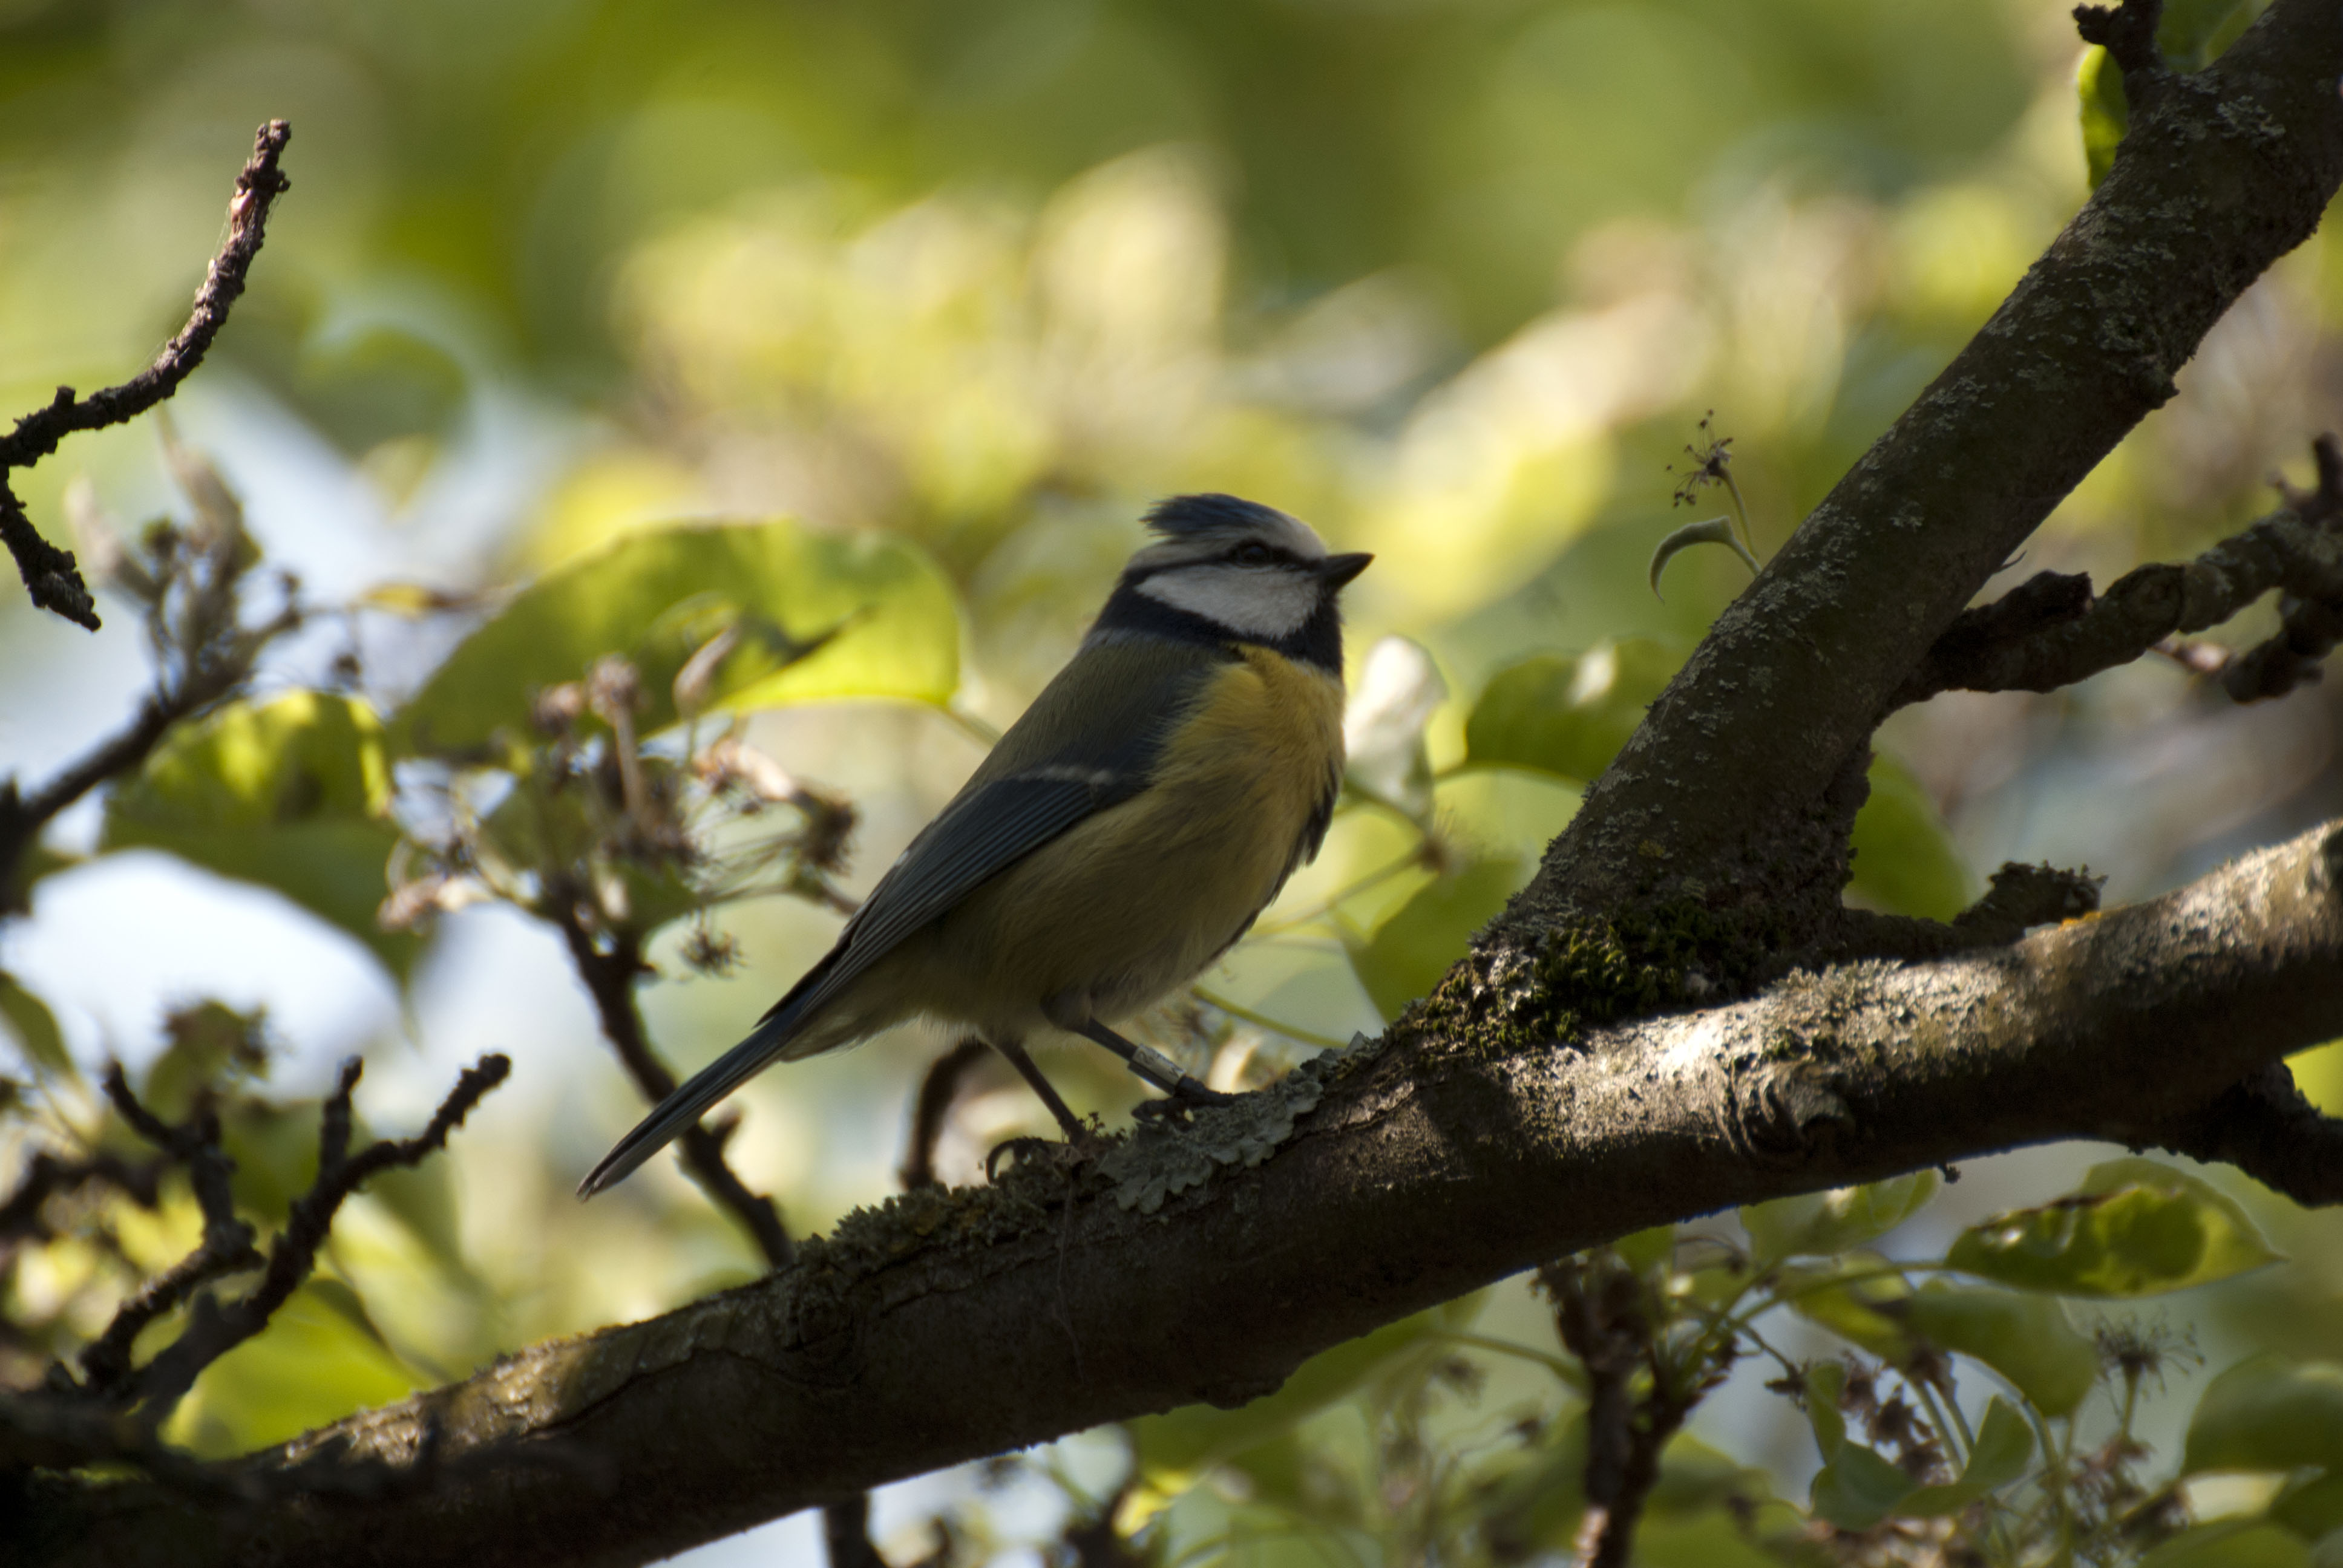
\includegraphics[width=0.8\textwidth]{data/Mésange_bleue_Descartes.jpg} \\
    \vspace{0.3cm}
    {\small Illustration – Mésange bleue observée à proximité du mâle 4}


    \vfill

    {\large ENS de Lyon\\
    L3 Biosciences\\
    Second semestre de l'année 2024-2025\par}
\end{titlepage}

{
\setcounter{tocdepth}{2}
\tableofcontents
}
\newpage

Pour pouvoir tricoter le document :

\begin{Shaded}
\begin{Highlighting}[]
\NormalTok{knitr}\SpecialCharTok{::}\NormalTok{opts\_chunk}\SpecialCharTok{$}\FunctionTok{set}\NormalTok{(}
  \AttributeTok{fig.width =} \DecValTok{6}\NormalTok{,       }\CommentTok{\# largeur en pouces (\textasciitilde{}15.2 cm)}
  \AttributeTok{fig.height =} \DecValTok{4}\NormalTok{,      }\CommentTok{\# hauteur en pouces}
  \AttributeTok{fig.align =} \StringTok{"center"}\NormalTok{,}\CommentTok{\# centre les graphiques}
  \AttributeTok{tidy.opts =} \FunctionTok{list}\NormalTok{(}\AttributeTok{width.cutoff =} \DecValTok{70}\NormalTok{),}
  \AttributeTok{dev =} \StringTok{"cairo\_pdf"} \CommentTok{\# necessite que le package cairo soit installe}
\NormalTok{)}
\end{Highlighting}
\end{Shaded}

\section{Importation des données et des
bibliothèques}\label{importation-des-donnuxe9es-et-des-bibliothuxe8ques}

Import des bibliothèques utilisées:

\begin{Shaded}
\begin{Highlighting}[]
\FunctionTok{library}\NormalTok{(tidyverse)}
\end{Highlighting}
\end{Shaded}

\begin{verbatim}
## -- Attaching core tidyverse packages ------------------------ tidyverse 2.0.0 --
## v dplyr     1.1.4     v readr     2.1.5
## v forcats   1.0.0     v stringr   1.5.1
## v ggplot2   3.5.2     v tibble    3.2.1
## v lubridate 1.9.4     v tidyr     1.3.1
## v purrr     1.0.4     
## -- Conflicts ------------------------------------------ tidyverse_conflicts() --
## x dplyr::filter() masks stats::filter()
## x dplyr::lag()    masks stats::lag()
## i Use the conflicted package (<http://conflicted.r-lib.org/>) to force all conflicts to become errors
\end{verbatim}

\begin{Shaded}
\begin{Highlighting}[]
\FunctionTok{library}\NormalTok{(dplyr)}
\FunctionTok{library}\NormalTok{(tidyr)}
\FunctionTok{library}\NormalTok{(readxl)}
\FunctionTok{library}\NormalTok{(openxlsx)}
\FunctionTok{library}\NormalTok{(here)}
\end{Highlighting}
\end{Shaded}

\begin{verbatim}
## here() starts at D:/Scolarité/ENS/L3/Biosciences_S6/TP Ecologie/Projet_mesanges
\end{verbatim}

\begin{Shaded}
\begin{Highlighting}[]
\FunctionTok{library}\NormalTok{(AER)}
\end{Highlighting}
\end{Shaded}

\begin{verbatim}
## Le chargement a nécessité le package : car
## Le chargement a nécessité le package : carData
## 
## Attachement du package : 'car'
## 
## L'objet suivant est masqué depuis 'package:dplyr':
## 
##     recode
## 
## L'objet suivant est masqué depuis 'package:purrr':
## 
##     some
## 
## Le chargement a nécessité le package : lmtest
## Le chargement a nécessité le package : zoo
## 
## Attachement du package : 'zoo'
## 
## Les objets suivants sont masqués depuis 'package:base':
## 
##     as.Date, as.Date.numeric
## 
## Le chargement a nécessité le package : sandwich
## Le chargement a nécessité le package : survival
\end{verbatim}

\begin{Shaded}
\begin{Highlighting}[]
\FunctionTok{library}\NormalTok{(brms)}
\end{Highlighting}
\end{Shaded}

\begin{verbatim}
## Le chargement a nécessité le package : Rcpp
## Loading 'brms' package (version 2.22.0). Useful instructions
## can be found by typing help('brms'). A more detailed introduction
## to the package is available through vignette('brms_overview').
## 
## Attachement du package : 'brms'
## 
## L'objet suivant est masqué depuis 'package:survival':
## 
##     kidney
## 
## L'objet suivant est masqué depuis 'package:stats':
## 
##     ar
\end{verbatim}

\begin{Shaded}
\begin{Highlighting}[]
\FunctionTok{library}\NormalTok{(DescTools)}
\end{Highlighting}
\end{Shaded}

\begin{verbatim}
## 
## Attachement du package : 'DescTools'
## 
## L'objet suivant est masqué depuis 'package:car':
## 
##     Recode
\end{verbatim}

\begin{Shaded}
\begin{Highlighting}[]
\FunctionTok{library}\NormalTok{(emmeans)}
\end{Highlighting}
\end{Shaded}

\begin{verbatim}
## Welcome to emmeans.
## Caution: You lose important information if you filter this package's results.
## See '? untidy'
\end{verbatim}

\begin{Shaded}
\begin{Highlighting}[]
\FunctionTok{library}\NormalTok{(rstatix)}
\end{Highlighting}
\end{Shaded}

\begin{verbatim}
## 
## Attachement du package : 'rstatix'
## 
## L'objet suivant est masqué depuis 'package:stats':
## 
##     filter
\end{verbatim}

\begin{Shaded}
\begin{Highlighting}[]
\FunctionTok{library}\NormalTok{(ggplot2)}
\FunctionTok{library}\NormalTok{(GGally)}
\end{Highlighting}
\end{Shaded}

\begin{verbatim}
## Registered S3 method overwritten by 'GGally':
##   method from   
##   +.gg   ggplot2
## 
## Attachement du package : 'GGally'
## 
## L'objet suivant est masqué depuis 'package:emmeans':
## 
##     pigs
\end{verbatim}

\begin{Shaded}
\begin{Highlighting}[]
\FunctionTok{library}\NormalTok{(ggpubr)}
\FunctionTok{library}\NormalTok{(ggsignif)}
\FunctionTok{library}\NormalTok{(patchwork)}
\FunctionTok{library}\NormalTok{(viridis)}
\end{Highlighting}
\end{Shaded}

\begin{verbatim}
## Le chargement a nécessité le package : viridisLite
\end{verbatim}

\begin{Shaded}
\begin{Highlighting}[]
\FunctionTok{library}\NormalTok{(ggeffects)}
\FunctionTok{library}\NormalTok{(gt)}

\FunctionTok{library}\NormalTok{(FactoMineR)}
\FunctionTok{library}\NormalTok{(factoextra)}
\end{Highlighting}
\end{Shaded}

\begin{verbatim}
## Welcome! Want to learn more? See two factoextra-related books at https://goo.gl/ve3WBa
\end{verbatim}

\section{Création du plan d'échantillonnage et importation des
données}\label{cruxe9ation-du-plan-duxe9chantillonnage-et-importation-des-donnuxe9es}

\subsection{Création du plan
d'échantillonnage}\label{cruxe9ation-du-plan-duxe9chantillonnage}

\begin{Shaded}
\begin{Highlighting}[]
\NormalTok{chant }\OtherTok{=} \FunctionTok{c}\NormalTok{(}\StringTok{"Bleu\_sans1"}\NormalTok{, }\StringTok{"Bleu\_sans2"}\NormalTok{, }\StringTok{"Bleu\_sans3"}\NormalTok{, }\StringTok{"Bleu\_court1"}\NormalTok{, }\StringTok{"Bleu\_court2"}\NormalTok{, }\StringTok{"Bleu\_court3"}\NormalTok{, }\StringTok{"Bleu\_long1"}\NormalTok{, }\StringTok{"Bleu\_long2"}\NormalTok{, }\StringTok{"Bleu\_long3"}\NormalTok{, }\StringTok{"Charbo\_2notes1"}\NormalTok{, }\StringTok{"Charbo\_2notes2"}\NormalTok{, }\StringTok{"Charbo\_2notes3"}\NormalTok{, }\StringTok{"Charbo\_2notes\_inv1"}\NormalTok{, }\StringTok{"Charbo\_2notes\_inv2"}\NormalTok{, }\StringTok{"Charbo\_2notes\_inv3"}\NormalTok{, }\StringTok{"Charbo\_3notes1"}\NormalTok{, }\StringTok{"Charbo\_3notes2"}\NormalTok{, }\StringTok{"Charbo\_3notes3"}\NormalTok{, }\StringTok{"Charbo\_3notes\_inv1"}\NormalTok{, }\StringTok{"Charbo\_3notes\_inv2"}\NormalTok{, }\StringTok{"Charbo\_3notes\_inv3"}\NormalTok{, }\StringTok{"Troglo1"}\NormalTok{, }\StringTok{"Troglo2"}\NormalTok{, }\StringTok{"Troglo3"}\NormalTok{)}

\NormalTok{plan }\OtherTok{=} \FunctionTok{matrix}\NormalTok{(}\DecValTok{0}\NormalTok{, }\AttributeTok{nrow=}\DecValTok{3}\SpecialCharTok{*}\DecValTok{24}\NormalTok{, }\AttributeTok{ncol=}\DecValTok{4}\NormalTok{)}
\FunctionTok{colnames}\NormalTok{(plan) }\OtherTok{=} \FunctionTok{c}\NormalTok{(}\StringTok{"Mâle 1 (parc)"}\NormalTok{, }\StringTok{"Mâle 2 (rue)"}\NormalTok{, }\StringTok{"Mâle 3 (sud)"}\NormalTok{, }\StringTok{"Mâle 4 (nord)"}\NormalTok{)}
  
\ControlFlowTok{for}\NormalTok{(i }\ControlFlowTok{in} \DecValTok{1}\SpecialCharTok{:}\DecValTok{4}\NormalTok{) \{}
\NormalTok{  plan[}\DecValTok{1}\SpecialCharTok{:}\DecValTok{24}\NormalTok{, i] }\OtherTok{\textless{}{-}} \FunctionTok{sample}\NormalTok{(chant)}
\NormalTok{  plan[}\DecValTok{25}\SpecialCharTok{:}\DecValTok{48}\NormalTok{, i] }\OtherTok{\textless{}{-}} \FunctionTok{sample}\NormalTok{(chant)}
\NormalTok{  plan[}\DecValTok{49}\SpecialCharTok{:}\DecValTok{72}\NormalTok{, i] }\OtherTok{\textless{}{-}} \FunctionTok{sample}\NormalTok{(chant)}
\NormalTok{\} }

\FunctionTok{write.xlsx}\NormalTok{(plan, }\AttributeTok{file =} \FunctionTok{here}\NormalTok{(}\StringTok{"output"}\NormalTok{, }\StringTok{"Plan\_echantillonnage.xlsx"}\NormalTok{))}
\end{Highlighting}
\end{Shaded}

\subsection{Importation des données}\label{importation-des-donnuxe9es}

Importation des données conservées dans un data frame.

\begin{Shaded}
\begin{Highlighting}[]
\NormalTok{data\_mesanges }\OtherTok{\textless{}{-}} \FunctionTok{read\_excel}\NormalTok{(}\FunctionTok{here}\NormalTok{(}\StringTok{"data"}\NormalTok{, }\StringTok{"TP\_mesange\_donnees\_nettoyees.xlsx"}\NormalTok{))}
\end{Highlighting}
\end{Shaded}

Création d'un deuxième data frame à partir des données brutes, qui aura
vocation à être ensuite modifié au gré des analyses que l'on souhaitera
faire.

\begin{Shaded}
\begin{Highlighting}[]
\NormalTok{data\_mesanges\_modifiee }\OtherTok{\textless{}{-}} \FunctionTok{read\_excel}\NormalTok{(}\FunctionTok{here}\NormalTok{(}\StringTok{"data"}\NormalTok{, }\StringTok{"TP\_mesange\_donnees\_nettoyees.xlsx"}\NormalTok{))}

\NormalTok{data\_mesanges\_modifiee }\OtherTok{\textless{}{-}}\NormalTok{ data\_mesanges\_modifiee }\SpecialCharTok{\%\textgreater{}\%} \FunctionTok{mutate}\NormalTok{(}
  \AttributeTok{Jour =} \FunctionTok{as.factor}\NormalTok{(Jour),}
  \AttributeTok{Son =} \FunctionTok{as.factor}\NormalTok{(Son),}
  \AttributeTok{Minute =} \FunctionTok{as.numeric}\NormalTok{(Minute), }
  \AttributeTok{Temperature =} \FunctionTok{as.numeric}\NormalTok{(Temperature), }
  \AttributeTok{Pluie =} \FunctionTok{as.numeric}\NormalTok{(Pluie), }
  \AttributeTok{Ensoleillement =} \FunctionTok{as.numeric}\NormalTok{(Ensoleillement), }
  \AttributeTok{Nombre\_passage =} \FunctionTok{as.numeric}\NormalTok{(Nombre\_passage), }
  \AttributeTok{Latence\_approche\_charbo =} \FunctionTok{as.numeric}\NormalTok{(Latence\_approche\_charbo), }
  \AttributeTok{Latence\_chant\_charbo =} \FunctionTok{as.numeric}\NormalTok{(Latence\_chant\_charbo), }
  \AttributeTok{Dist\_min\_charbo =} \FunctionTok{as.numeric}\NormalTok{(Dist\_min\_charbo), }
  \AttributeTok{Pre\_2 =} \FunctionTok{as.numeric}\NormalTok{(Pre\_2), }
  \AttributeTok{Post\_2 =} \FunctionTok{as.numeric}\NormalTok{(Post\_2), }
  \AttributeTok{Pre\_3 =} \FunctionTok{as.numeric}\NormalTok{(Pre\_3), }
  \AttributeTok{Post\_3 =} \FunctionTok{as.numeric}\NormalTok{(Post\_3), }
  \AttributeTok{Latence\_approche\_bleue =} \FunctionTok{as.numeric}\NormalTok{(Latence\_approche\_bleue), }
  \AttributeTok{Latence\_chant\_bleue =} \FunctionTok{as.numeric}\NormalTok{(Latence\_chant\_bleue), }
  \AttributeTok{Dist\_min\_bleue =} \FunctionTok{as.numeric}\NormalTok{(Dist\_min\_bleue), }
  \AttributeTok{Sans\_trilles\_pre =} \FunctionTok{as.numeric}\NormalTok{(Sans\_trilles\_pre), }
  \AttributeTok{Sans\_trilles\_post =} \FunctionTok{as.numeric}\NormalTok{(Sans\_trilles\_post), }
  \AttributeTok{Court\_pre =} \FunctionTok{as.numeric}\NormalTok{(Court\_pre), }
  \AttributeTok{Court\_post =} \FunctionTok{as.numeric}\NormalTok{(Court\_post), }
  \AttributeTok{Long\_pre =} \FunctionTok{as.numeric}\NormalTok{(Long\_pre), }
  \AttributeTok{Long\_post =} \FunctionTok{as.numeric}\NormalTok{(Long\_post))}
\end{Highlighting}
\end{Shaded}

\begin{verbatim}
## Warning: There were 6 warnings in `mutate()`.
## The first warning was:
## i In argument: `Latence_approche_charbo = as.numeric(Latence_approche_charbo)`.
## Caused by warning:
## ! NAs introduits lors de la conversion automatique
## i Run `dplyr::last_dplyr_warnings()` to see the 5 remaining warnings.
\end{verbatim}

Il ne sera pas toujours pertinent pour nos analyses séparer les
différents types de chants au sein d'une même espèce (comme les chants à
deux notes et à trois notes chez la mésange charbonnière).

On modifie donc ce tableau en ajoutant des colonnes contenant pour
chacune des diffusions la somme des réponses, soit avant soit après
diffusion, pour les deux espèces de mésanges.

Nombre de strophes pré et post diffusion chez la mésange charbonnière

\begin{Shaded}
\begin{Highlighting}[]
\NormalTok{data\_mesanges\_modifiee}\SpecialCharTok{$}\NormalTok{somme\_charbo\_pre }\OtherTok{\textless{}{-}} \FunctionTok{as.numeric}\NormalTok{(data\_mesanges\_modifiee}\SpecialCharTok{$}\NormalTok{Pre\_2) }\SpecialCharTok{+} \FunctionTok{as.numeric}\NormalTok{(data\_mesanges\_modifiee}\SpecialCharTok{$}\NormalTok{Pre\_3)}
\NormalTok{data\_mesanges\_modifiee}\SpecialCharTok{$}\NormalTok{somme\_charbo\_post}\OtherTok{\textless{}{-}} \FunctionTok{as.numeric}\NormalTok{(data\_mesanges\_modifiee}\SpecialCharTok{$}\NormalTok{Post\_2) }\SpecialCharTok{+} \FunctionTok{as.numeric}\NormalTok{(data\_mesanges\_modifiee}\SpecialCharTok{$}\NormalTok{Post\_3)}
\end{Highlighting}
\end{Shaded}

Nombre de strophes pré et post diffusion chez la mésange bleue

\begin{Shaded}
\begin{Highlighting}[]
\NormalTok{data\_mesanges\_modifiee}\SpecialCharTok{$}\NormalTok{somme\_bleue\_pre }\OtherTok{\textless{}{-}}\FunctionTok{as.numeric}\NormalTok{(data\_mesanges\_modifiee}\SpecialCharTok{$}\NormalTok{Sans\_trilles\_pre) }\SpecialCharTok{+} \FunctionTok{as.numeric}\NormalTok{(data\_mesanges\_modifiee}\SpecialCharTok{$}\NormalTok{Court\_pre) }\SpecialCharTok{+} \FunctionTok{as.numeric}\NormalTok{(data\_mesanges\_modifiee}\SpecialCharTok{$}\NormalTok{Long\_pre) }
\NormalTok{data\_mesanges\_modifiee}\SpecialCharTok{$}\NormalTok{somme\_bleue\_post }\OtherTok{\textless{}{-}} \FunctionTok{as.numeric}\NormalTok{(data\_mesanges\_modifiee}\SpecialCharTok{$}\NormalTok{Sans\_trilles\_post) }\SpecialCharTok{+} \FunctionTok{as.numeric}\NormalTok{(data\_mesanges\_modifiee}\SpecialCharTok{$}\NormalTok{Court\_post) }\SpecialCharTok{+} \FunctionTok{as.numeric}\NormalTok{(data\_mesanges\_modifiee}\SpecialCharTok{$}\NormalTok{Long\_post)}
\end{Highlighting}
\end{Shaded}

De même, d'autres colonnes seront nécessaires.

Nombre de strophes totales (c'est-à-dire la somme des strophes pré et
post diffusion) chez les deux espèces de mésanges bleue et charbonnière.

\begin{Shaded}
\begin{Highlighting}[]
\NormalTok{data\_mesanges\_modifiee}\SpecialCharTok{$}\NormalTok{nombre\_charbo\_total }\OtherTok{\textless{}{-}}\NormalTok{ data\_mesanges\_modifiee}\SpecialCharTok{$}\NormalTok{somme\_charbo\_pre }\SpecialCharTok{+}\NormalTok{ data\_mesanges\_modifiee}\SpecialCharTok{$}\NormalTok{somme\_charbo\_post}
\NormalTok{data\_mesanges\_modifiee}\SpecialCharTok{$}\NormalTok{nombre\_bleue\_total }\OtherTok{\textless{}{-}}\NormalTok{ data\_mesanges\_modifiee}\SpecialCharTok{$}\NormalTok{somme\_bleue\_pre }\SpecialCharTok{+}\NormalTok{ data\_mesanges\_modifiee}\SpecialCharTok{$}\NormalTok{somme\_bleue\_post}
\end{Highlighting}
\end{Shaded}

Nombre de strophes pré et post diffusion chez les deux espèces de
mésanges confondues.

\begin{Shaded}
\begin{Highlighting}[]
\NormalTok{data\_mesanges\_modifiee}\SpecialCharTok{$}\NormalTok{nombre\_total\_pre }\OtherTok{\textless{}{-}}\NormalTok{ data\_mesanges\_modifiee}\SpecialCharTok{$}\NormalTok{somme\_charbo\_pre }\SpecialCharTok{+}\NormalTok{ data\_mesanges\_modifiee}\SpecialCharTok{$}\NormalTok{somme\_bleue\_pre}
\NormalTok{data\_mesanges\_modifiee}\SpecialCharTok{$}\NormalTok{nombre\_total\_post }\OtherTok{\textless{}{-}}\NormalTok{ data\_mesanges\_modifiee}\SpecialCharTok{$}\NormalTok{somme\_charbo\_post }\SpecialCharTok{+}\NormalTok{ data\_mesanges\_modifiee}\SpecialCharTok{$}\NormalTok{somme\_bleue\_post}
\end{Highlighting}
\end{Shaded}

Nombre de strophes totales (c'est-à-dire la somme des strophes pré et
post diffusion) chez les deux espèces de mésanges confondues.

\begin{Shaded}
\begin{Highlighting}[]
\NormalTok{data\_mesanges\_modifiee}\SpecialCharTok{$}\NormalTok{nombre\_total }\OtherTok{\textless{}{-}}\NormalTok{ data\_mesanges\_modifiee}\SpecialCharTok{$}\NormalTok{nombre\_total\_pre }\SpecialCharTok{+}\NormalTok{ data\_mesanges\_modifiee}\SpecialCharTok{$}\NormalTok{nombre\_total\_post}
\end{Highlighting}
\end{Shaded}

Ajout de nouvelles variables: Création d'une colonne comprenant le temps
total d'observation des mésanges. Elle a été calculé à partir de la
colone minute qui représente les temps converti en minutes (7h45
correspondant au temps 0 de chaque jour). Et donc le temps total
d'observations des journées précédentes a été ajouté à chaque journées.
Nous avons négligé dans ce calcul les moments où il n'y avait pas
d'observations au cours de la journée comme les pauses méridiennes ou
encore les moments où on s'est arbité de l'averse.

\begin{Shaded}
\begin{Highlighting}[]
\NormalTok{data\_mesanges\_modifiee}\SpecialCharTok{$}\NormalTok{temps\_total }\OtherTok{\textless{}{-}} \FunctionTok{as.numeric}\NormalTok{(data\_mesanges\_modifiee}\SpecialCharTok{$}\NormalTok{Minute)}
\NormalTok{data\_mesanges\_modifiee }\OtherTok{\textless{}{-}}\NormalTok{ data\_mesanges\_modifiee }\SpecialCharTok{\%\textgreater{}\%}
  \FunctionTok{mutate}\NormalTok{(}\AttributeTok{temps\_total =} \FunctionTok{as.numeric}\NormalTok{(Minute) }\SpecialCharTok{+} \FunctionTok{case\_when}\NormalTok{(}
\NormalTok{    Jour }\SpecialCharTok{==} \DecValTok{1} \SpecialCharTok{\textasciitilde{}}\NormalTok{ (}\DecValTok{494} \SpecialCharTok{{-}} \DecValTok{2}\NormalTok{),}
\NormalTok{    Jour }\SpecialCharTok{==} \DecValTok{2} \SpecialCharTok{\textasciitilde{}}\NormalTok{ (}\DecValTok{473} \SpecialCharTok{{-}} \DecValTok{7}\NormalTok{) }\SpecialCharTok{+}\NormalTok{ (}\DecValTok{494} \SpecialCharTok{{-}} \DecValTok{2}\NormalTok{),}
\NormalTok{    Jour }\SpecialCharTok{==} \DecValTok{3} \SpecialCharTok{\textasciitilde{}}\NormalTok{ (}\DecValTok{618} \SpecialCharTok{{-}} \DecValTok{363}\NormalTok{) }\SpecialCharTok{+}\NormalTok{ (}\DecValTok{473} \SpecialCharTok{{-}} \DecValTok{7}\NormalTok{) }\SpecialCharTok{+}\NormalTok{ (}\DecValTok{494} \SpecialCharTok{{-}} \DecValTok{2}\NormalTok{),}
\NormalTok{    Jour }\SpecialCharTok{==} \DecValTok{4} \SpecialCharTok{\textasciitilde{}}\NormalTok{ (}\DecValTok{463} \SpecialCharTok{{-}} \DecValTok{83}\NormalTok{) }\SpecialCharTok{+}\NormalTok{ (}\DecValTok{618} \SpecialCharTok{{-}} \DecValTok{363}\NormalTok{) }\SpecialCharTok{+}\NormalTok{ (}\DecValTok{473} \SpecialCharTok{{-}} \DecValTok{7}\NormalTok{) }\SpecialCharTok{+}\NormalTok{ (}\DecValTok{494} \SpecialCharTok{{-}} \DecValTok{2}\NormalTok{),}
\NormalTok{  ))}
\end{Highlighting}
\end{Shaded}

\newpage

\section{Exploration des données -- Réalisation d'analyses en
composantes principales
(ACP)}\label{exploration-des-donnuxe9es-ruxe9alisation-danalyses-en-composantes-principales-acp}

Sur le terrain, nous avons pu émettre différentes hypothèses, comme nous
le verrons par la suite. Cependant, afin de s'assurer que nous n'avions
pas oublié de corrélation entre données, nous avons commencé par réalisé
différentes ACP afin d'observer ou non, de telles corrélation.

\subsection{Création du data.frame pour les
ACP}\label{cruxe9ation-du-data.frame-pour-les-acp}

On en transforme les données quantitatives afin qu'elles soient
utilisables par la fonction PCA().

\begin{Shaded}
\begin{Highlighting}[]
\NormalTok{df\_PCA }\OtherTok{\textless{}{-}} \FunctionTok{read\_xlsx}\NormalTok{(}\FunctionTok{here}\NormalTok{(}\StringTok{"data"}\NormalTok{, }\StringTok{\textquotesingle{}TP\_mesange\_donnees\_nettoyees.xlsx\textquotesingle{}}\NormalTok{))}

\NormalTok{df\_PCA }\OtherTok{\textless{}{-}}\NormalTok{ df\_PCA }\SpecialCharTok{\%\textgreater{}\%} \FunctionTok{mutate}\NormalTok{(}
  \AttributeTok{Minute =} \FunctionTok{as.numeric}\NormalTok{(Minute), }
  \AttributeTok{Temperature =} \FunctionTok{as.numeric}\NormalTok{(Temperature), }
  \AttributeTok{Pluie =} \FunctionTok{as.numeric}\NormalTok{(Pluie), }
  \AttributeTok{Ensoleillement =} \FunctionTok{as.numeric}\NormalTok{(Ensoleillement), }
  \AttributeTok{Nombre\_passage =} \FunctionTok{as.numeric}\NormalTok{(Nombre\_passage), }
  \AttributeTok{Latence\_approche\_charbo =} \FunctionTok{as.numeric}\NormalTok{(Latence\_approche\_charbo) }\SpecialCharTok{{-}} \DecValTok{60}\NormalTok{, }
  \AttributeTok{Latence\_chant\_charbo =} \FunctionTok{as.numeric}\NormalTok{(Latence\_chant\_charbo) }\SpecialCharTok{{-}} \DecValTok{60}\NormalTok{, }
  \AttributeTok{Pre\_2 =} \FunctionTok{as.numeric}\NormalTok{(Pre\_2), }
  \AttributeTok{Post\_2 =} \FunctionTok{as.numeric}\NormalTok{(Post\_2), }
  \AttributeTok{Pre\_3 =} \FunctionTok{as.numeric}\NormalTok{(Pre\_3), }
  \AttributeTok{Post\_3 =} \FunctionTok{as.numeric}\NormalTok{(Post\_3), }
  \AttributeTok{Latence\_approche\_bleue =} \FunctionTok{as.numeric}\NormalTok{(Latence\_approche\_bleue), }
  \AttributeTok{Latence\_chant\_bleue =} \FunctionTok{as.numeric}\NormalTok{(Latence\_chant\_bleue),}
  \AttributeTok{Sans\_trilles\_pre =} \FunctionTok{as.numeric}\NormalTok{(Sans\_trilles\_pre) }\SpecialCharTok{{-}} \DecValTok{60}\NormalTok{, }
  \AttributeTok{Sans\_trilles\_post =} \FunctionTok{as.numeric}\NormalTok{(Sans\_trilles\_post) }\SpecialCharTok{{-}} \DecValTok{60}\NormalTok{, }
  \AttributeTok{Court\_pre =} \FunctionTok{as.numeric}\NormalTok{(Court\_pre), }
  \AttributeTok{Court\_post =} \FunctionTok{as.numeric}\NormalTok{(Court\_post), }
  \AttributeTok{Long\_pre =} \FunctionTok{as.numeric}\NormalTok{(Long\_pre), }
  \AttributeTok{Long\_post =} \FunctionTok{as.numeric}\NormalTok{(Long\_post))}
\end{Highlighting}
\end{Shaded}

\begin{verbatim}
## Warning: There were 4 warnings in `mutate()`.
## The first warning was:
## i In argument: `Latence_approche_charbo = as.numeric(Latence_approche_charbo) -
##   60`.
## Caused by warning:
## ! NAs introduits lors de la conversion automatique
## i Run `dplyr::last_dplyr_warnings()` to see the 3 remaining warnings.
\end{verbatim}

Puis on le modifie de manière à ce que l'absence de chant ou d'approche
d'une mésange corresponde à une latence supérieure à la latence réelle
d'observation (on ajoute une seconde à ce temps, le mâle 1 ayant une
fois chanté très peu de temps après la fin de l'observation).

\begin{Shaded}
\begin{Highlighting}[]
\ControlFlowTok{for}\NormalTok{ (i }\ControlFlowTok{in} \DecValTok{1}\SpecialCharTok{:}\DecValTok{139}\NormalTok{) \{}
  \ControlFlowTok{if}\NormalTok{ (}\FunctionTok{is.na}\NormalTok{(df\_PCA}\SpecialCharTok{$}\NormalTok{Latence\_approche\_charbo[i])) \{}
\NormalTok{    df\_PCA}\SpecialCharTok{$}\NormalTok{Latence\_approche\_charbo[i] }\OtherTok{=} \DecValTok{301}
\NormalTok{  \}}
  \ControlFlowTok{if}\NormalTok{ (}\FunctionTok{is.na}\NormalTok{(df\_PCA}\SpecialCharTok{$}\NormalTok{Latence\_approche\_bleue[i])) \{}
\NormalTok{    df\_PCA}\SpecialCharTok{$}\NormalTok{Latence\_approche\_bleue[i] }\OtherTok{=} \DecValTok{301}
\NormalTok{  \}}
  \ControlFlowTok{if}\NormalTok{ (}\FunctionTok{is.na}\NormalTok{(df\_PCA}\SpecialCharTok{$}\NormalTok{Latence\_chant\_charbo[i])) \{}
\NormalTok{    df\_PCA}\SpecialCharTok{$}\NormalTok{Latence\_chant\_charbo[i] }\OtherTok{=} \DecValTok{301}
\NormalTok{  \}}
  \ControlFlowTok{if}\NormalTok{ (}\FunctionTok{is.na}\NormalTok{(df\_PCA}\SpecialCharTok{$}\NormalTok{Latence\_chant\_bleue[i])) \{}
\NormalTok{    df\_PCA}\SpecialCharTok{$}\NormalTok{Latence\_chant\_bleue[i] }\OtherTok{=} \DecValTok{301}
\NormalTok{  \}}
\NormalTok{\}}
\end{Highlighting}
\end{Shaded}

\subsection{Première approche : prise en compte de tous les
paramètres}\label{premiuxe8re-approche-prise-en-compte-de-tous-les-paramuxe8tres}

On prend en compte tous les paramètres quantitatifs. Pour ce faire, on
met les colonnes non quantitatives en premier pour sélectionner
facilement les colonnes quantitatives par la suite.

\begin{Shaded}
\begin{Highlighting}[]
\NormalTok{explo\_PCA\_charbo }\OtherTok{\textless{}{-}}\NormalTok{ df\_PCA[, }\FunctionTok{c}\NormalTok{(}\StringTok{"Jour"}\NormalTok{, }\StringTok{"Male"}\NormalTok{, }\StringTok{"Son"}\NormalTok{, }\StringTok{"Minute"}\NormalTok{, }\StringTok{"Temperature"}\NormalTok{, }\StringTok{"Pluie"}\NormalTok{, }\StringTok{"Vent"}\NormalTok{, }\StringTok{"Ensoleillement"}\NormalTok{, }\StringTok{"Nombre\_passage"}\NormalTok{, }\StringTok{"Latence\_approche\_charbo"}\NormalTok{, }\StringTok{"Latence\_chant\_charbo"}\NormalTok{, }\StringTok{"Pre\_2"}\NormalTok{, }\StringTok{"Post\_2"}\NormalTok{, }\StringTok{"Pre\_3"}\NormalTok{, }\StringTok{"Post\_3"}\NormalTok{)]}


\NormalTok{explo\_PCA\_bleue }\OtherTok{\textless{}{-}}\NormalTok{ df\_PCA[, }\FunctionTok{c}\NormalTok{(}\StringTok{"Jour"}\NormalTok{, }\StringTok{"Male"}\NormalTok{, }\StringTok{"Son"}\NormalTok{, }\StringTok{"Minute"}\NormalTok{, }\StringTok{"Temperature"}\NormalTok{, }\StringTok{"Pluie"}\NormalTok{, }\StringTok{"Vent"}\NormalTok{, }\StringTok{"Ensoleillement"}\NormalTok{, }\StringTok{"Nombre\_passage"}\NormalTok{, }\StringTok{"Latence\_approche\_bleue"}\NormalTok{, }\StringTok{"Latence\_chant\_bleue"}\NormalTok{, }\StringTok{"Sans\_trilles\_pre"}\NormalTok{, }\StringTok{"Sans\_trilles\_post"}\NormalTok{, }\StringTok{"Court\_pre"}\NormalTok{, }\StringTok{"Court\_post"}\NormalTok{, }\StringTok{"Long\_pre"}\NormalTok{, }\StringTok{"Long\_post"}\NormalTok{)]}

\NormalTok{df\_PCA}\SpecialCharTok{$}\NormalTok{Somme\_pre\_charbo }\OtherTok{\textless{}{-}} \FunctionTok{rowSums}\NormalTok{(df\_PCA[, }\FunctionTok{c}\NormalTok{(}\StringTok{"Pre\_2"}\NormalTok{, }\StringTok{"Pre\_3"}\NormalTok{)], }\AttributeTok{na.rm =} \ConstantTok{TRUE}\NormalTok{)}
\NormalTok{df\_PCA}\SpecialCharTok{$}\NormalTok{Somme\_pre\_bleue }\OtherTok{\textless{}{-}} \FunctionTok{rowSums}\NormalTok{(df\_PCA[, }\FunctionTok{c}\NormalTok{(}\StringTok{"Sans\_trilles\_pre"}\NormalTok{, }\StringTok{"Court\_pre"}\NormalTok{, }\StringTok{"Long\_pre"}\NormalTok{)], }\AttributeTok{na.rm =} \ConstantTok{TRUE}\NormalTok{)}
\end{Highlighting}
\end{Shaded}

Puis on fait une première observation des données.

\begin{Shaded}
\begin{Highlighting}[]
\NormalTok{explo\_PCA\_charbo }\OtherTok{\textless{}{-}} \FunctionTok{PCA}\NormalTok{(explo\_PCA\_charbo[, }\DecValTok{4}\SpecialCharTok{:}\DecValTok{14}\NormalTok{], }\AttributeTok{scale.unit =} \ConstantTok{TRUE}\NormalTok{)}
\end{Highlighting}
\end{Shaded}

\begin{center}
\includegraphics{Compte_rendu_TP_ecologie_Mesanges_files/figure-latex/unnamed-chunk-15-1} \end{center}

\begin{center}
\includegraphics{Compte_rendu_TP_ecologie_Mesanges_files/figure-latex/unnamed-chunk-15-2} \end{center}

\begin{Shaded}
\begin{Highlighting}[]
\FunctionTok{fviz\_screeplot}\NormalTok{(explo\_PCA\_charbo, }\AttributeTok{ncp =}\DecValTok{5}\NormalTok{) }\SpecialCharTok{+} \FunctionTok{ggtitle}\NormalTok{(}\StringTok{"Pourcentage de la variance expliquée par les dimensions, pour l\textquotesingle{}ACP associant }\SpecialCharTok{\textbackslash{}n}\StringTok{ variables métérologiques et comportement des mésanges charbonnières"}\NormalTok{) }\SpecialCharTok{+} \FunctionTok{theme}\NormalTok{(}\AttributeTok{plot.title =} \FunctionTok{element\_text}\NormalTok{(}\AttributeTok{size =} \DecValTok{10}\NormalTok{, }\AttributeTok{hjust =} \FloatTok{0.5}\NormalTok{))}
\end{Highlighting}
\end{Shaded}

\begin{center}\includegraphics{Compte_rendu_TP_ecologie_Mesanges_files/figure-latex/unnamed-chunk-15-3} \end{center}

\begin{Shaded}
\begin{Highlighting}[]
\NormalTok{explo\_PCA\_bleue }\OtherTok{\textless{}{-}} \FunctionTok{PCA}\NormalTok{(explo\_PCA\_bleue[, }\DecValTok{4}\SpecialCharTok{:}\DecValTok{16}\NormalTok{], }\AttributeTok{scale.unit =} \ConstantTok{TRUE}\NormalTok{)}
\end{Highlighting}
\end{Shaded}

\begin{center}\includegraphics{Compte_rendu_TP_ecologie_Mesanges_files/figure-latex/unnamed-chunk-15-4} \end{center}

\begin{center}\includegraphics{Compte_rendu_TP_ecologie_Mesanges_files/figure-latex/unnamed-chunk-15-5} \end{center}

\begin{Shaded}
\begin{Highlighting}[]
\FunctionTok{fviz\_screeplot}\NormalTok{(explo\_PCA\_bleue, }\AttributeTok{ncp =}\DecValTok{5}\NormalTok{) }\SpecialCharTok{+} \FunctionTok{ggtitle}\NormalTok{(}\StringTok{"Pourcentage de la variance expliquée par les dimensions, pour l\textquotesingle{}ACP associant }\SpecialCharTok{\textbackslash{}n}\StringTok{ variables métérologiques et comportement des mésanges bleues"}\NormalTok{) }\SpecialCharTok{+} \FunctionTok{theme}\NormalTok{(}\AttributeTok{plot.title =} \FunctionTok{element\_text}\NormalTok{(}\AttributeTok{size =} \DecValTok{10}\NormalTok{, }\AttributeTok{hjust =} \FloatTok{0.5}\NormalTok{))}
\end{Highlighting}
\end{Shaded}

\begin{center}\includegraphics{Compte_rendu_TP_ecologie_Mesanges_files/figure-latex/unnamed-chunk-15-6} \end{center}

On observe alors que la pluie est correlée positivement au nombre de
passages et négativement à l'ensoleillement et à la température. Cela
montre bien la réalité du terrain, puisque les jours passant, les
conditions métérologiques se sont dégradées. De plus, on observe une
corrélation négative entre les latences et le nombre de strophes
chantées : plus un oiseau arrive tard moins il est susceptible de
chanter.

Une fois cette première approche, nous avons cherché à visualiser
l'effet de plusieurs facteurs, à savoir les données métérologiques, le
chant diffusé ou le jour.

\subsection{Deuxième approche, recherche d'un effet des données
métérologique.}\label{deuxiuxe8me-approche-recherche-dun-effet-des-donnuxe9es-muxe9tuxe9rologique.}

\begin{Shaded}
\begin{Highlighting}[]
\NormalTok{explo\_PCA\_meteo }\OtherTok{\textless{}{-}} \FunctionTok{PCA}\NormalTok{(df\_PCA[, }\FunctionTok{c}\NormalTok{(}\StringTok{"Temperature"}\NormalTok{, }\StringTok{"Pluie"}\NormalTok{, }\StringTok{"Vent"}\NormalTok{, }\StringTok{"Ensoleillement"}\NormalTok{)])}
\end{Highlighting}
\end{Shaded}

\begin{center}
\includegraphics{Compte_rendu_TP_ecologie_Mesanges_files/figure-latex/unnamed-chunk-16-1} \end{center}

\begin{center}
\includegraphics{Compte_rendu_TP_ecologie_Mesanges_files/figure-latex/unnamed-chunk-16-2} \end{center}

\begin{Shaded}
\begin{Highlighting}[]
\FunctionTok{fviz\_screeplot}\NormalTok{(explo\_PCA\_meteo) }\SpecialCharTok{+} \FunctionTok{ggtitle}\NormalTok{(}\StringTok{"Variance du jeu de données métérologiques"}\NormalTok{)}
\end{Highlighting}
\end{Shaded}

\begin{center}\includegraphics{Compte_rendu_TP_ecologie_Mesanges_files/figure-latex/unnamed-chunk-16-3} \end{center}

\begin{Shaded}
\begin{Highlighting}[]
\FunctionTok{fviz\_contrib}\NormalTok{(explo\_PCA\_meteo, }\AttributeTok{choice =} \StringTok{"var"}\NormalTok{, }\AttributeTok{axes =} \DecValTok{1}\NormalTok{) }\SpecialCharTok{+} \FunctionTok{ggtitle}\NormalTok{(}\StringTok{"Participation des variables à la dimension 1 de l\textquotesingle{}ACP métérologique"}\NormalTok{)}
\end{Highlighting}
\end{Shaded}

\begin{center}\includegraphics{Compte_rendu_TP_ecologie_Mesanges_files/figure-latex/unnamed-chunk-16-4} \end{center}

\begin{Shaded}
\begin{Highlighting}[]
\NormalTok{explo\_PCA\_meteo\_charbo }\OtherTok{\textless{}{-}} \FunctionTok{PCA}\NormalTok{(df\_PCA[, }\FunctionTok{c}\NormalTok{(}\StringTok{"Temperature"}\NormalTok{, }\StringTok{"Pluie"}\NormalTok{, }\StringTok{"Vent"}\NormalTok{, }\StringTok{"Ensoleillement"}\NormalTok{, }\StringTok{"Somme\_pre\_charbo"}\NormalTok{)], }\AttributeTok{scale.unit =} \ConstantTok{TRUE}\NormalTok{)}
\end{Highlighting}
\end{Shaded}

\begin{center}\includegraphics{Compte_rendu_TP_ecologie_Mesanges_files/figure-latex/unnamed-chunk-16-5} \end{center}

\begin{center}\includegraphics{Compte_rendu_TP_ecologie_Mesanges_files/figure-latex/unnamed-chunk-16-6} \end{center}

\begin{Shaded}
\begin{Highlighting}[]
\FunctionTok{fviz\_screeplot}\NormalTok{(explo\_PCA\_meteo\_charbo, }\AttributeTok{ncp =}\DecValTok{5}\NormalTok{)  }\SpecialCharTok{+} \FunctionTok{ggtitle}\NormalTok{(}\StringTok{"Variance du jeu de données métérologiques associée aux réponses des mésanges charbonnières"}\NormalTok{) }\SpecialCharTok{+} \FunctionTok{theme}\NormalTok{(}\AttributeTok{plot.title =} \FunctionTok{element\_text}\NormalTok{(}\AttributeTok{size =} \DecValTok{10}\NormalTok{, }\AttributeTok{hjust =} \FloatTok{0.5}\NormalTok{))}
\end{Highlighting}
\end{Shaded}

\begin{center}\includegraphics{Compte_rendu_TP_ecologie_Mesanges_files/figure-latex/unnamed-chunk-16-7} \end{center}

\begin{Shaded}
\begin{Highlighting}[]
\FunctionTok{fviz\_contrib}\NormalTok{(explo\_PCA\_meteo\_charbo, }\AttributeTok{choice =} \StringTok{"var"}\NormalTok{, }\AttributeTok{axes =} \DecValTok{1}\NormalTok{) }\SpecialCharTok{+} \FunctionTok{ggtitle}\NormalTok{(}\StringTok{"Participation des variables à la dimension 1 de l\textquotesingle{}ACP associant }\SpecialCharTok{\textbackslash{}n}\StringTok{ données météorologiques et réponses des mésanges charbonnières"}\NormalTok{) }\SpecialCharTok{+} \FunctionTok{theme}\NormalTok{(}\AttributeTok{plot.title =} \FunctionTok{element\_text}\NormalTok{(}\AttributeTok{size =} \DecValTok{10}\NormalTok{, }\AttributeTok{hjust =} \FloatTok{0.5}\NormalTok{))}
\end{Highlighting}
\end{Shaded}

\begin{center}\includegraphics{Compte_rendu_TP_ecologie_Mesanges_files/figure-latex/unnamed-chunk-16-8} \end{center}

\begin{Shaded}
\begin{Highlighting}[]
\NormalTok{explo\_PCA\_meteo\_bleue }\OtherTok{\textless{}{-}} \FunctionTok{PCA}\NormalTok{(df\_PCA[, }\FunctionTok{c}\NormalTok{(}\StringTok{"Temperature"}\NormalTok{, }\StringTok{"Pluie"}\NormalTok{, }\StringTok{"Vent"}\NormalTok{, }\StringTok{"Ensoleillement"}\NormalTok{, }\StringTok{"Somme\_pre\_bleue"}\NormalTok{)], }\AttributeTok{scale.unit =} \ConstantTok{TRUE}\NormalTok{)}
\end{Highlighting}
\end{Shaded}

\begin{center}\includegraphics{Compte_rendu_TP_ecologie_Mesanges_files/figure-latex/unnamed-chunk-16-9} \end{center}

\begin{center}\includegraphics{Compte_rendu_TP_ecologie_Mesanges_files/figure-latex/unnamed-chunk-16-10} \end{center}

\begin{Shaded}
\begin{Highlighting}[]
\FunctionTok{fviz\_screeplot}\NormalTok{(explo\_PCA\_meteo\_bleue, }\AttributeTok{ncp =}\DecValTok{5}\NormalTok{) }\SpecialCharTok{+} \FunctionTok{ggtitle}\NormalTok{(}\StringTok{"Variance du jeu de données métérologiques associée aux réponses des mésanges bleues"}\NormalTok{) }\SpecialCharTok{+} \FunctionTok{theme}\NormalTok{(}\AttributeTok{plot.title =} \FunctionTok{element\_text}\NormalTok{(}\AttributeTok{size =} \DecValTok{10}\NormalTok{, }\AttributeTok{hjust =} \FloatTok{0.5}\NormalTok{))}
\end{Highlighting}
\end{Shaded}

\begin{center}\includegraphics{Compte_rendu_TP_ecologie_Mesanges_files/figure-latex/unnamed-chunk-16-11} \end{center}

\begin{Shaded}
\begin{Highlighting}[]
\FunctionTok{fviz\_contrib}\NormalTok{(explo\_PCA\_meteo\_bleue, }\AttributeTok{choice =} \StringTok{"var"}\NormalTok{, }\AttributeTok{axes =} \DecValTok{1}\NormalTok{) }\SpecialCharTok{+} \FunctionTok{ggtitle}\NormalTok{(}\StringTok{"Participation des variables à la dimension 1 de l\textquotesingle{}ACP associant }\SpecialCharTok{\textbackslash{}n}\StringTok{ données météorologiques et réponses des mésanges bleues"}\NormalTok{) }\SpecialCharTok{+} \FunctionTok{theme}\NormalTok{(}\AttributeTok{plot.title =} \FunctionTok{element\_text}\NormalTok{(}\AttributeTok{size =} \DecValTok{10}\NormalTok{, }\AttributeTok{hjust =} \FloatTok{0.5}\NormalTok{))}
\end{Highlighting}
\end{Shaded}

\begin{center}\includegraphics{Compte_rendu_TP_ecologie_Mesanges_files/figure-latex/unnamed-chunk-16-12} \end{center}

Sur ces graphiques, on observe une anti-corrélation entre la somme des
chants et la pluviométrie, plus marquée pour les mésanges bleues que
pour les charbonnières. L'effet de la pluie sur le nombre de strophes
chantés sera testé par la suite.

\subsection{Troisième approche, recherche d'un effet de variable
qualitative}\label{troisiuxe8me-approche-recherche-dun-effet-de-variable-qualitative}

Dans un premier temps, l'analyse comportementale a utilisé le jeu de
donné au sein duquel les mésanges n'ayant pas été vu et/ou entendues
présentent des latences respectives de 301 secondes. En effet, le nombre
de données était très faible si l'on enlevait ces données. Dans un
second temps, un analyse comportementale des charbonnières a été tentée
en enlevant les lignes où des données étaient manquantes afin d'étudier
des corrélations uniquement entre des données observées.

\subsubsection{Création des PCA}\label{cruxe9ation-des-pca}

\begin{Shaded}
\begin{Highlighting}[]
\NormalTok{df\_comp\_charbo }\OtherTok{\textless{}{-}}\NormalTok{ df\_PCA[, }\FunctionTok{c}\NormalTok{(}\StringTok{"Jour"}\NormalTok{, }\StringTok{"Son"}\NormalTok{, }\StringTok{"Latence\_approche\_charbo"}\NormalTok{, }\StringTok{"Latence\_chant\_charbo"}\NormalTok{, }\StringTok{"Pre\_2"}\NormalTok{, }\StringTok{"Post\_2"}\NormalTok{, }\StringTok{"Pre\_3"}\NormalTok{, }\StringTok{"Post\_3"}\NormalTok{)]}

\NormalTok{df\_comp\_charbo}\SpecialCharTok{$}\NormalTok{Jour }\OtherTok{\textless{}{-}} \FunctionTok{as.factor}\NormalTok{(df\_comp\_charbo}\SpecialCharTok{$}\NormalTok{Jour)}
\NormalTok{df\_comp\_charbo}\SpecialCharTok{$}\NormalTok{Son }\OtherTok{\textless{}{-}} \FunctionTok{as.factor}\NormalTok{(df\_comp\_charbo}\SpecialCharTok{$}\NormalTok{Son)}

\NormalTok{PCA\_comp\_charbo }\OtherTok{\textless{}{-}} \FunctionTok{PCA}\NormalTok{(df\_comp\_charbo[, }\DecValTok{3}\SpecialCharTok{:}\DecValTok{8}\NormalTok{], }\AttributeTok{scale.unit =} \ConstantTok{TRUE}\NormalTok{)}
\end{Highlighting}
\end{Shaded}

\begin{center}
\includegraphics{Compte_rendu_TP_ecologie_Mesanges_files/figure-latex/unnamed-chunk-17-1} \end{center}

\begin{center}
\includegraphics{Compte_rendu_TP_ecologie_Mesanges_files/figure-latex/unnamed-chunk-17-2} \end{center}

\begin{Shaded}
\begin{Highlighting}[]
\FunctionTok{fviz\_screeplot}\NormalTok{(PCA\_comp\_charbo, }\AttributeTok{ncp =} \DecValTok{5}\NormalTok{) }\SpecialCharTok{+} \FunctionTok{ggtitle}\NormalTok{(}\StringTok{"Sources de variance au sein du comportement }\SpecialCharTok{\textbackslash{}n}\StringTok{ des mésanges charbonnières"}\NormalTok{)}
\end{Highlighting}
\end{Shaded}

\begin{center}\includegraphics{Compte_rendu_TP_ecologie_Mesanges_files/figure-latex/unnamed-chunk-17-3} \end{center}

\begin{Shaded}
\begin{Highlighting}[]
\FunctionTok{fviz\_contrib}\NormalTok{(PCA\_comp\_charbo, }\AttributeTok{choice =} \StringTok{"var"}\NormalTok{, }\AttributeTok{axes =} \DecValTok{1}\NormalTok{) }\SpecialCharTok{+} \FunctionTok{ggtitle}\NormalTok{(}\StringTok{"Contribution des variables à la dimension 1 de l\textquotesingle{}ACP portant sur le comportement }\SpecialCharTok{\textbackslash{}n}\StringTok{ des mésanges charbonnières"}\NormalTok{) }\SpecialCharTok{+} \FunctionTok{theme}\NormalTok{(}\AttributeTok{plot.title =} \FunctionTok{element\_text}\NormalTok{(}\AttributeTok{size =} \DecValTok{10}\NormalTok{, }\AttributeTok{hjust =} \FloatTok{0.5}\NormalTok{))}
\end{Highlighting}
\end{Shaded}

\begin{center}\includegraphics{Compte_rendu_TP_ecologie_Mesanges_files/figure-latex/unnamed-chunk-17-4} \end{center}

\begin{Shaded}
\begin{Highlighting}[]
\FunctionTok{fviz\_contrib}\NormalTok{(PCA\_comp\_charbo, }\AttributeTok{choice =} \StringTok{"var"}\NormalTok{, }\AttributeTok{axes =} \DecValTok{2}\NormalTok{) }\SpecialCharTok{+} \FunctionTok{ggtitle}\NormalTok{(}\StringTok{"Contribution des variables à la dimension 2 de l\textquotesingle{}ACP portant sur le comportement des mésanges charbonnières"}\NormalTok{) }\SpecialCharTok{+} \FunctionTok{theme}\NormalTok{(}\AttributeTok{plot.title =} \FunctionTok{element\_text}\NormalTok{(}\AttributeTok{size =} \DecValTok{10}\NormalTok{, }\AttributeTok{hjust =} \FloatTok{0.5}\NormalTok{))}
\end{Highlighting}
\end{Shaded}

\begin{center}\includegraphics{Compte_rendu_TP_ecologie_Mesanges_files/figure-latex/unnamed-chunk-17-5} \end{center}

\begin{Shaded}
\begin{Highlighting}[]
\FunctionTok{fviz\_contrib}\NormalTok{(PCA\_comp\_charbo, }\AttributeTok{choice =} \StringTok{"var"}\NormalTok{, }\AttributeTok{axes =} \DecValTok{3}\NormalTok{) }\SpecialCharTok{+} \FunctionTok{ggtitle}\NormalTok{(}\StringTok{"Contribution des variables à la dimension 3 de l\textquotesingle{}ACP portant sur le comportement }\SpecialCharTok{\textbackslash{}n}\StringTok{ des mésanges charbonnières"}\NormalTok{) }\SpecialCharTok{+} \FunctionTok{theme}\NormalTok{(}\AttributeTok{plot.title =} \FunctionTok{element\_text}\NormalTok{(}\AttributeTok{size =} \DecValTok{10}\NormalTok{, }\AttributeTok{hjust =} \FloatTok{0.5}\NormalTok{))}
\end{Highlighting}
\end{Shaded}

\begin{center}\includegraphics{Compte_rendu_TP_ecologie_Mesanges_files/figure-latex/unnamed-chunk-17-6} \end{center}

\begin{Shaded}
\begin{Highlighting}[]
\FunctionTok{fviz\_contrib}\NormalTok{(PCA\_comp\_charbo, }\AttributeTok{choice =} \StringTok{"var"}\NormalTok{, }\AttributeTok{axes =} \DecValTok{4}\NormalTok{) }\SpecialCharTok{+} \FunctionTok{ggtitle}\NormalTok{(}\StringTok{"Contribution des variables à la dimension 4 de l\textquotesingle{}ACP portant sur le comportement }\SpecialCharTok{\textbackslash{}n}\StringTok{ des mésanges charbonnières"}\NormalTok{) }\SpecialCharTok{+} \FunctionTok{theme}\NormalTok{(}\AttributeTok{plot.title =} \FunctionTok{element\_text}\NormalTok{(}\AttributeTok{size =} \DecValTok{10}\NormalTok{, }\AttributeTok{hjust =} \FloatTok{0.5}\NormalTok{))}
\end{Highlighting}
\end{Shaded}

\begin{center}\includegraphics{Compte_rendu_TP_ecologie_Mesanges_files/figure-latex/unnamed-chunk-17-7} \end{center}

Les 4 premières dimensions expliquent la majorité de la variabilité du
jeu de données. De plus, certaines dimensions forment des groupes
cohérents (ici, la dimension une est formée par l'ensemble des variables
liées à la réaction des mésanges, à savoir les latences et le nombre de
strophes chantées après diffusion).

\begin{Shaded}
\begin{Highlighting}[]
\NormalTok{df\_comp\_bleue }\OtherTok{\textless{}{-}}\NormalTok{ df\_PCA[, }\FunctionTok{c}\NormalTok{(}\StringTok{"Jour"}\NormalTok{, }\StringTok{"Son"}\NormalTok{, }\StringTok{"Latence\_approche\_bleue"}\NormalTok{, }\StringTok{"Latence\_chant\_bleue"}\NormalTok{, }\StringTok{"Sans\_trilles\_pre"}\NormalTok{, }\StringTok{"Sans\_trilles\_post"}\NormalTok{, }\StringTok{"Court\_pre"}\NormalTok{, }\StringTok{"Court\_post"}\NormalTok{, }\StringTok{"Long\_pre"}\NormalTok{, }\StringTok{"Long\_post"}\NormalTok{)]}

\NormalTok{df\_comp\_bleue}\SpecialCharTok{$}\NormalTok{Jour }\OtherTok{\textless{}{-}} \FunctionTok{as.factor}\NormalTok{(df\_comp\_bleue}\SpecialCharTok{$}\NormalTok{Jour)}
\NormalTok{df\_comp\_bleue}\SpecialCharTok{$}\NormalTok{Son }\OtherTok{\textless{}{-}} \FunctionTok{as.factor}\NormalTok{(df\_comp\_bleue}\SpecialCharTok{$}\NormalTok{Son)}

\NormalTok{PCA\_comp\_bleue }\OtherTok{\textless{}{-}} \FunctionTok{PCA}\NormalTok{(df\_comp\_bleue[, }\DecValTok{3}\SpecialCharTok{:}\DecValTok{10}\NormalTok{], }\AttributeTok{scale.unit =} \ConstantTok{TRUE}\NormalTok{)}
\end{Highlighting}
\end{Shaded}

\begin{center}
\includegraphics{Compte_rendu_TP_ecologie_Mesanges_files/figure-latex/unnamed-chunk-18-1} \end{center}

\begin{center}
\includegraphics{Compte_rendu_TP_ecologie_Mesanges_files/figure-latex/unnamed-chunk-18-2} \end{center}

\begin{Shaded}
\begin{Highlighting}[]
\FunctionTok{fviz\_screeplot}\NormalTok{(PCA\_comp\_bleue, }\AttributeTok{ncp =} \DecValTok{10}\NormalTok{)}\SpecialCharTok{+} \FunctionTok{ggtitle}\NormalTok{(}\StringTok{"Sources de variance au sein du comportement }\SpecialCharTok{\textbackslash{}n}\StringTok{ des mésanges bleues"}\NormalTok{)}
\end{Highlighting}
\end{Shaded}

\begin{center}\includegraphics{Compte_rendu_TP_ecologie_Mesanges_files/figure-latex/unnamed-chunk-18-3} \end{center}

\begin{Shaded}
\begin{Highlighting}[]
\FunctionTok{fviz\_contrib}\NormalTok{(PCA\_comp\_bleue, }\AttributeTok{choice =} \StringTok{"var"}\NormalTok{, }\AttributeTok{axes =} \DecValTok{1}\NormalTok{) }\SpecialCharTok{+} \FunctionTok{ggtitle}\NormalTok{(}\StringTok{"Contribution des variables à la dimension 1 de l\textquotesingle{}ACP portant sur le comportement }\SpecialCharTok{\textbackslash{}n}\StringTok{ des mésanges bleues"}\NormalTok{) }\SpecialCharTok{+} \FunctionTok{theme}\NormalTok{(}\AttributeTok{plot.title =} \FunctionTok{element\_text}\NormalTok{(}\AttributeTok{size =} \DecValTok{10}\NormalTok{, }\AttributeTok{hjust =} \FloatTok{0.5}\NormalTok{))}
\end{Highlighting}
\end{Shaded}

\begin{center}\includegraphics{Compte_rendu_TP_ecologie_Mesanges_files/figure-latex/unnamed-chunk-18-4} \end{center}

\begin{Shaded}
\begin{Highlighting}[]
\FunctionTok{fviz\_contrib}\NormalTok{(PCA\_comp\_bleue, }\AttributeTok{choice =} \StringTok{"var"}\NormalTok{, }\AttributeTok{axes =} \DecValTok{2}\NormalTok{) }\SpecialCharTok{+} \FunctionTok{ggtitle}\NormalTok{(}\StringTok{"Contribution des variables à la dimension 2 de l\textquotesingle{}ACP portant sur le comportement }\SpecialCharTok{\textbackslash{}n}\StringTok{ des mésanges bleues"}\NormalTok{) }\SpecialCharTok{+} \FunctionTok{theme}\NormalTok{(}\AttributeTok{plot.title =} \FunctionTok{element\_text}\NormalTok{(}\AttributeTok{size =} \DecValTok{10}\NormalTok{, }\AttributeTok{hjust =} \FloatTok{0.5}\NormalTok{))}
\end{Highlighting}
\end{Shaded}

\begin{center}\includegraphics{Compte_rendu_TP_ecologie_Mesanges_files/figure-latex/unnamed-chunk-18-5} \end{center}

\begin{Shaded}
\begin{Highlighting}[]
\FunctionTok{fviz\_contrib}\NormalTok{(PCA\_comp\_bleue, }\AttributeTok{choice =} \StringTok{"var"}\NormalTok{, }\AttributeTok{axes =} \DecValTok{3}\NormalTok{) }\SpecialCharTok{+} \FunctionTok{ggtitle}\NormalTok{(}\StringTok{"Contribution des variables à la dimension 3 de l\textquotesingle{}ACP portant sur le comportement}\SpecialCharTok{\textbackslash{}n}\StringTok{ des mésanges bleues"}\NormalTok{) }\SpecialCharTok{+} \FunctionTok{theme}\NormalTok{(}\AttributeTok{plot.title =} \FunctionTok{element\_text}\NormalTok{(}\AttributeTok{size =} \DecValTok{10}\NormalTok{, }\AttributeTok{hjust =} \FloatTok{0.5}\NormalTok{))}
\end{Highlighting}
\end{Shaded}

\begin{center}\includegraphics{Compte_rendu_TP_ecologie_Mesanges_files/figure-latex/unnamed-chunk-18-6} \end{center}

\begin{Shaded}
\begin{Highlighting}[]
\FunctionTok{fviz\_contrib}\NormalTok{(PCA\_comp\_bleue, }\AttributeTok{choice =} \StringTok{"var"}\NormalTok{, }\AttributeTok{axes =} \DecValTok{4}\NormalTok{) }\SpecialCharTok{+} \FunctionTok{ggtitle}\NormalTok{(}\StringTok{"Contribution des variables à la dimension 4 de l\textquotesingle{}ACP portant sur le comportement }\SpecialCharTok{\textbackslash{}n}\StringTok{ des mésanges bleues"}\NormalTok{) }\SpecialCharTok{+} \FunctionTok{theme}\NormalTok{(}\AttributeTok{plot.title =} \FunctionTok{element\_text}\NormalTok{(}\AttributeTok{size =} \DecValTok{10}\NormalTok{, }\AttributeTok{hjust =} \FloatTok{0.5}\NormalTok{))}
\end{Highlighting}
\end{Shaded}

\begin{center}\includegraphics{Compte_rendu_TP_ecologie_Mesanges_files/figure-latex/unnamed-chunk-18-7} \end{center}

Une fois de plus, les quatre premières dimensions expliquent la majorité
de la variabilité du jeu de données. Cependant, cette fois-ci, il est
difficile de faire des liens entre les variables explicatives d'une
dimension.

\subsubsection{Recherche d'un effet du
chant}\label{recherche-dun-effet-du-chant}

On différencie les points en fonction du chant ayant été diffusé.

\begin{Shaded}
\begin{Highlighting}[]
\FunctionTok{fviz\_pca\_ind}\NormalTok{(PCA\_comp\_charbo,}
             \AttributeTok{axes =} \FunctionTok{c}\NormalTok{(}\DecValTok{1}\NormalTok{, }\DecValTok{2}\NormalTok{),}
             \AttributeTok{geom =} \StringTok{"point"}\NormalTok{,}
             \AttributeTok{habillage =}\NormalTok{ df\_comp\_charbo}\SpecialCharTok{$}\NormalTok{Son,}
             \AttributeTok{palette =} \FunctionTok{c}\NormalTok{(}\StringTok{"\#98F5FF"}\NormalTok{, }\StringTok{"\#53868B"}\NormalTok{, }\StringTok{"\#6495ED"}\NormalTok{, }\StringTok{"\#FFB90F"}\NormalTok{,}\StringTok{"\#CD950C"}\NormalTok{, }\StringTok{"\#FFD700"}\NormalTok{, }\StringTok{"\#8B7500"}\NormalTok{, }\StringTok{"\#8B4513"}\NormalTok{),}
             \AttributeTok{addEllipses =} \ConstantTok{TRUE}\NormalTok{,}
             \AttributeTok{mean.point =} \ConstantTok{FALSE}\NormalTok{) }\SpecialCharTok{+} 
  \FunctionTok{ggtitle}\NormalTok{(}\StringTok{"ACP des variables représentant la réponse des mésanges charbonnières,}\SpecialCharTok{\textbackslash{}n}\StringTok{ coloriées en fonction du chant diffusé"}\NormalTok{) }\SpecialCharTok{+} 
  \FunctionTok{theme}\NormalTok{(}\AttributeTok{plot.title =} \FunctionTok{element\_text}\NormalTok{(}\AttributeTok{size =} \DecValTok{10}\NormalTok{, }\AttributeTok{hjust =} \FloatTok{0.5}\NormalTok{))}
\end{Highlighting}
\end{Shaded}

\begin{center}
\includegraphics{Compte_rendu_TP_ecologie_Mesanges_files/figure-latex/unnamed-chunk-19-1} \end{center}

\begin{Shaded}
\begin{Highlighting}[]
\FunctionTok{fviz\_pca\_ind}\NormalTok{(PCA\_comp\_charbo,}
             \AttributeTok{axes =} \FunctionTok{c}\NormalTok{(}\DecValTok{2}\NormalTok{, }\DecValTok{3}\NormalTok{),}
             \AttributeTok{geom =} \StringTok{"point"}\NormalTok{,}
             \AttributeTok{habillage =}\NormalTok{ df\_comp\_charbo}\SpecialCharTok{$}\NormalTok{Son,}
             \AttributeTok{palette =} \FunctionTok{c}\NormalTok{(}\StringTok{"\#98F5FF"}\NormalTok{, }\StringTok{"\#53868B"}\NormalTok{, }\StringTok{"\#6495ED"}\NormalTok{, }\StringTok{"\#FFB90F"}\NormalTok{,}\StringTok{"\#CD950C"}\NormalTok{, }\StringTok{"\#FFD700"}\NormalTok{, }\StringTok{"\#8B7500"}\NormalTok{, }\StringTok{"\#8B4513"}\NormalTok{),}
             \AttributeTok{addEllipses =} \ConstantTok{TRUE}\NormalTok{,}
             \AttributeTok{mean.point =} \ConstantTok{FALSE}\NormalTok{) }\SpecialCharTok{+}
   \FunctionTok{ggtitle}\NormalTok{(}\StringTok{"ACP des variables représentant la réponse des mésanges charbonnières,}\SpecialCharTok{\textbackslash{}n}\StringTok{ coloriées en fonction du chant diffusé"}\NormalTok{) }\SpecialCharTok{+} 
  \FunctionTok{theme}\NormalTok{(}\AttributeTok{plot.title =} \FunctionTok{element\_text}\NormalTok{(}\AttributeTok{size =} \DecValTok{10}\NormalTok{, }\AttributeTok{hjust =} \FloatTok{0.5}\NormalTok{))}
\end{Highlighting}
\end{Shaded}

\begin{center}\includegraphics{Compte_rendu_TP_ecologie_Mesanges_files/figure-latex/unnamed-chunk-19-2} \end{center}

\begin{Shaded}
\begin{Highlighting}[]
\FunctionTok{fviz\_pca\_ind}\NormalTok{(PCA\_comp\_charbo,}
             \AttributeTok{axes =} \FunctionTok{c}\NormalTok{(}\DecValTok{3}\NormalTok{, }\DecValTok{4}\NormalTok{),}
             \AttributeTok{geom =} \StringTok{"point"}\NormalTok{,}
             \AttributeTok{habillage =}\NormalTok{ df\_comp\_charbo}\SpecialCharTok{$}\NormalTok{Son,}
             \AttributeTok{palette =} \FunctionTok{c}\NormalTok{(}\StringTok{"\#98F5FF"}\NormalTok{, }\StringTok{"\#53868B"}\NormalTok{, }\StringTok{"\#6495ED"}\NormalTok{, }\StringTok{"\#FFB90F"}\NormalTok{,}\StringTok{"\#CD950C"}\NormalTok{, }\StringTok{"\#FFD700"}\NormalTok{, }\StringTok{"\#8B7500"}\NormalTok{, }\StringTok{"\#8B4513"}\NormalTok{),}
             \AttributeTok{addEllipses =} \ConstantTok{TRUE}\NormalTok{,}
             \AttributeTok{mean.point =} \ConstantTok{FALSE}\NormalTok{) }\SpecialCharTok{+}
   \FunctionTok{ggtitle}\NormalTok{(}\StringTok{"ACP des variables représentant la réponse des mésanges charbonnières,}\SpecialCharTok{\textbackslash{}n}\StringTok{ coloriées en fonction du chant diffusé"}\NormalTok{) }\SpecialCharTok{+}
  \FunctionTok{theme}\NormalTok{(}\AttributeTok{plot.title =} \FunctionTok{element\_text}\NormalTok{(}\AttributeTok{size =} \DecValTok{10}\NormalTok{, }\AttributeTok{hjust =} \FloatTok{0.5}\NormalTok{))}
\end{Highlighting}
\end{Shaded}

\begin{center}\includegraphics{Compte_rendu_TP_ecologie_Mesanges_files/figure-latex/unnamed-chunk-19-3} \end{center}

On n'observe pas de regroupement de données disctincts des autres.
Ainsi, pour les mésanges charbonnières, il ne semble pas y avoir de
différence de réactions en fonction du type de chant diffusé.

\begin{Shaded}
\begin{Highlighting}[]
\FunctionTok{fviz\_pca\_ind}\NormalTok{(PCA\_comp\_bleue,}
             \AttributeTok{axes =} \FunctionTok{c}\NormalTok{(}\DecValTok{1}\NormalTok{, }\DecValTok{2}\NormalTok{),}
             \AttributeTok{geom =} \StringTok{"point"}\NormalTok{,}
             \AttributeTok{habillage =}\NormalTok{ df\_comp\_bleue}\SpecialCharTok{$}\NormalTok{Son,}
             \AttributeTok{palette =} \FunctionTok{c}\NormalTok{(}\StringTok{"\#98F5FF"}\NormalTok{, }\StringTok{"\#53868B"}\NormalTok{, }\StringTok{"\#6495ED"}\NormalTok{, }\StringTok{"\#FFB90F"}\NormalTok{,}\StringTok{"\#CD950C"}\NormalTok{, }\StringTok{"\#FFD700"}\NormalTok{, }\StringTok{"\#8B7500"}\NormalTok{, }\StringTok{"\#8B4513"}\NormalTok{),}
             \AttributeTok{addEllipses =} \ConstantTok{TRUE}\NormalTok{,}
             \AttributeTok{mean.point =} \ConstantTok{FALSE}\NormalTok{) }\SpecialCharTok{+} 
  \FunctionTok{ggtitle}\NormalTok{(}\StringTok{"ACP des variables représentant la réponse des mésanges bleues,}\SpecialCharTok{\textbackslash{}n}\StringTok{ coloriées en fonction du chant diffusé"}\NormalTok{) }\SpecialCharTok{+} 
  \FunctionTok{theme}\NormalTok{(}\AttributeTok{plot.title =} \FunctionTok{element\_text}\NormalTok{(}\AttributeTok{size =} \DecValTok{10}\NormalTok{, }\AttributeTok{hjust =} \FloatTok{0.5}\NormalTok{))}
\end{Highlighting}
\end{Shaded}

\begin{center}
\includegraphics{Compte_rendu_TP_ecologie_Mesanges_files/figure-latex/unnamed-chunk-20-1} \end{center}

\begin{Shaded}
\begin{Highlighting}[]
\FunctionTok{fviz\_pca\_ind}\NormalTok{(PCA\_comp\_bleue,}
             \AttributeTok{axes =} \FunctionTok{c}\NormalTok{(}\DecValTok{2}\NormalTok{, }\DecValTok{3}\NormalTok{),}
             \AttributeTok{geom =} \StringTok{"point"}\NormalTok{,}
             \AttributeTok{habillage =}\NormalTok{ df\_comp\_bleue}\SpecialCharTok{$}\NormalTok{Son,}
             \AttributeTok{palette =} \FunctionTok{c}\NormalTok{(}\StringTok{"\#98F5FF"}\NormalTok{, }\StringTok{"\#53868B"}\NormalTok{, }\StringTok{"\#6495ED"}\NormalTok{, }\StringTok{"\#FFB90F"}\NormalTok{,}\StringTok{"\#CD950C"}\NormalTok{, }\StringTok{"\#FFD700"}\NormalTok{, }\StringTok{"\#8B7500"}\NormalTok{, }\StringTok{"\#8B4513"}\NormalTok{),}
             \AttributeTok{addEllipses =} \ConstantTok{TRUE}\NormalTok{,}
             \AttributeTok{mean.point =} \ConstantTok{FALSE}\NormalTok{) }\SpecialCharTok{+}
   \FunctionTok{ggtitle}\NormalTok{(}\StringTok{"ACP des variables représentant la réponse des mésanges bleues,}\SpecialCharTok{\textbackslash{}n}\StringTok{ coloriées en fonction du chant diffusé"}\NormalTok{) }\SpecialCharTok{+} 
  \FunctionTok{theme}\NormalTok{(}\AttributeTok{plot.title =} \FunctionTok{element\_text}\NormalTok{(}\AttributeTok{size =} \DecValTok{10}\NormalTok{, }\AttributeTok{hjust =} \FloatTok{0.5}\NormalTok{))}
\end{Highlighting}
\end{Shaded}

\begin{center}\includegraphics{Compte_rendu_TP_ecologie_Mesanges_files/figure-latex/unnamed-chunk-20-2} \end{center}

\begin{Shaded}
\begin{Highlighting}[]
\FunctionTok{fviz\_pca\_ind}\NormalTok{(PCA\_comp\_bleue,}
             \AttributeTok{axes =} \FunctionTok{c}\NormalTok{(}\DecValTok{3}\NormalTok{, }\DecValTok{4}\NormalTok{),}
             \AttributeTok{geom =} \StringTok{"point"}\NormalTok{,}
             \AttributeTok{habillage =}\NormalTok{ df\_comp\_bleue}\SpecialCharTok{$}\NormalTok{Son,}
             \AttributeTok{palette =} \FunctionTok{c}\NormalTok{(}\StringTok{"\#98F5FF"}\NormalTok{, }\StringTok{"\#53868B"}\NormalTok{, }\StringTok{"\#6495ED"}\NormalTok{, }\StringTok{"\#FFB90F"}\NormalTok{,}\StringTok{"\#CD950C"}\NormalTok{, }\StringTok{"\#FFD700"}\NormalTok{, }\StringTok{"\#8B7500"}\NormalTok{, }\StringTok{"\#8B4513"}\NormalTok{),}
             \AttributeTok{addEllipses =} \ConstantTok{TRUE}\NormalTok{,}
             \AttributeTok{mean.point =} \ConstantTok{FALSE}\NormalTok{) }\SpecialCharTok{+}
   \FunctionTok{ggtitle}\NormalTok{(}\StringTok{"ACP des variables représentant la réponse des mésanges bleues,}\SpecialCharTok{\textbackslash{}n}\StringTok{ coloriées en fonction du chant diffusé"}\NormalTok{) }\SpecialCharTok{+}
  \FunctionTok{theme}\NormalTok{(}\AttributeTok{plot.title =} \FunctionTok{element\_text}\NormalTok{(}\AttributeTok{size =} \DecValTok{10}\NormalTok{, }\AttributeTok{hjust =} \FloatTok{0.5}\NormalTok{))}
\end{Highlighting}
\end{Shaded}

\begin{center}\includegraphics{Compte_rendu_TP_ecologie_Mesanges_files/figure-latex/unnamed-chunk-20-3} \end{center}

De même, on n'observe pas de regroupement de données disctincts des
autres. Il ne semble donc pas y avoir de différence de réactions en
fonction du type de chant diffusé.

\subsubsection{Recherche d'un effet du
jour}\label{recherche-dun-effet-du-jour}

On différencie les points en fonction du jour de diffusion.

\begin{Shaded}
\begin{Highlighting}[]
\FunctionTok{fviz\_pca\_ind}\NormalTok{(PCA\_comp\_charbo,}
             \AttributeTok{axes =} \FunctionTok{c}\NormalTok{(}\DecValTok{1}\NormalTok{, }\DecValTok{2}\NormalTok{),}
             \AttributeTok{geom =} \StringTok{"point"}\NormalTok{,}
             \AttributeTok{habillage =}\NormalTok{ df\_comp\_charbo}\SpecialCharTok{$}\NormalTok{Jour,}
             \AttributeTok{palette =} \FunctionTok{c}\NormalTok{(}\StringTok{"\#00CD00"}\NormalTok{, }\StringTok{"hotpink2"}\NormalTok{, }\StringTok{"\#EE2C2C"}\NormalTok{, }\StringTok{"\#00BFFF"}\NormalTok{),}
             \AttributeTok{addEllipses =} \ConstantTok{TRUE}\NormalTok{,}
             \AttributeTok{mean.point =} \ConstantTok{FALSE}\NormalTok{) }\SpecialCharTok{+}
   \FunctionTok{ggtitle}\NormalTok{(}\StringTok{"ACP des variables représentant la réponse des mésanges charbonnières,}\SpecialCharTok{\textbackslash{}n}\StringTok{ coloriées en fonction du jour de diffusion"}\NormalTok{) }\SpecialCharTok{+}
  \FunctionTok{theme}\NormalTok{(}\AttributeTok{plot.title =} \FunctionTok{element\_text}\NormalTok{(}\AttributeTok{size =} \DecValTok{10}\NormalTok{, }\AttributeTok{hjust =} \FloatTok{0.5}\NormalTok{))}
\end{Highlighting}
\end{Shaded}

\begin{center}
\includegraphics{Compte_rendu_TP_ecologie_Mesanges_files/figure-latex/unnamed-chunk-21-1} \end{center}

\begin{Shaded}
\begin{Highlighting}[]
\FunctionTok{fviz\_pca\_ind}\NormalTok{(PCA\_comp\_charbo,}
             \AttributeTok{axes =} \FunctionTok{c}\NormalTok{(}\DecValTok{2}\NormalTok{, }\DecValTok{3}\NormalTok{),}
             \AttributeTok{geom =} \StringTok{"point"}\NormalTok{,}
             \AttributeTok{habillage =}\NormalTok{ df\_comp\_charbo}\SpecialCharTok{$}\NormalTok{Jour,}
             \AttributeTok{palette =} \FunctionTok{c}\NormalTok{(}\StringTok{"\#00CD00"}\NormalTok{, }\StringTok{"hotpink2"}\NormalTok{, }\StringTok{"\#EE2C2C"}\NormalTok{, }\StringTok{"\#00BFFF"}\NormalTok{),}
             \AttributeTok{addEllipses =} \ConstantTok{TRUE}\NormalTok{,}
             \AttributeTok{mean.point =} \ConstantTok{FALSE}\NormalTok{) }\SpecialCharTok{+}
   \FunctionTok{ggtitle}\NormalTok{(}\StringTok{"ACP des variables représentant la réponse des mésanges charbonnières,}\SpecialCharTok{\textbackslash{}n}\StringTok{ coloriées en fonction du jour de diffusion"}\NormalTok{) }\SpecialCharTok{+}
  \FunctionTok{theme}\NormalTok{(}\AttributeTok{plot.title =} \FunctionTok{element\_text}\NormalTok{(}\AttributeTok{size =} \DecValTok{10}\NormalTok{, }\AttributeTok{hjust =} \FloatTok{0.5}\NormalTok{))}
\end{Highlighting}
\end{Shaded}

\begin{center}\includegraphics{Compte_rendu_TP_ecologie_Mesanges_files/figure-latex/unnamed-chunk-21-2} \end{center}

\begin{Shaded}
\begin{Highlighting}[]
\FunctionTok{fviz\_pca\_ind}\NormalTok{(PCA\_comp\_charbo,}
             \AttributeTok{axes =} \FunctionTok{c}\NormalTok{(}\DecValTok{3}\NormalTok{, }\DecValTok{4}\NormalTok{),}
             \AttributeTok{geom =} \StringTok{"point"}\NormalTok{,}
             \AttributeTok{habillage =}\NormalTok{ df\_comp\_charbo}\SpecialCharTok{$}\NormalTok{Jour,}
             \AttributeTok{palette =} \FunctionTok{c}\NormalTok{(}\StringTok{"\#00CD00"}\NormalTok{, }\StringTok{"hotpink2"}\NormalTok{, }\StringTok{"\#EE2C2C"}\NormalTok{, }\StringTok{"\#00BFFF"}\NormalTok{),}
             \AttributeTok{addEllipses =} \ConstantTok{TRUE}\NormalTok{,}
             \AttributeTok{mean.point =} \ConstantTok{FALSE}\NormalTok{) }\SpecialCharTok{+}
   \FunctionTok{ggtitle}\NormalTok{(}\StringTok{"ACP des variables représentant la réponse des mésanges charbonnières,}\SpecialCharTok{\textbackslash{}n}\StringTok{ coloriées en fonction du jour de diffusion"}\NormalTok{) }\SpecialCharTok{+}
  \FunctionTok{theme}\NormalTok{(}\AttributeTok{plot.title =} \FunctionTok{element\_text}\NormalTok{(}\AttributeTok{size =} \DecValTok{10}\NormalTok{, }\AttributeTok{hjust =} \FloatTok{0.5}\NormalTok{))}
\end{Highlighting}
\end{Shaded}

\begin{center}\includegraphics{Compte_rendu_TP_ecologie_Mesanges_files/figure-latex/unnamed-chunk-21-3} \end{center}

Encore une fois, on n'observe pas de regroupement de données disctincts
des autres. Il ne semble donc pas y avoir de différence de réactions en
fonction du jour de diffusion.

\begin{Shaded}
\begin{Highlighting}[]
\FunctionTok{fviz\_pca\_ind}\NormalTok{(PCA\_comp\_bleue,}
             \AttributeTok{axes =} \FunctionTok{c}\NormalTok{(}\DecValTok{1}\NormalTok{, }\DecValTok{2}\NormalTok{),}
             \AttributeTok{geom =} \StringTok{"point"}\NormalTok{,}
             \AttributeTok{habillage =}\NormalTok{ df\_comp\_bleue}\SpecialCharTok{$}\NormalTok{Jour,}
             \AttributeTok{palette =} \FunctionTok{c}\NormalTok{(}\StringTok{"\#00CD00"}\NormalTok{, }\StringTok{"hotpink2"}\NormalTok{, }\StringTok{"\#EE2C2C"}\NormalTok{, }\StringTok{"\#00BFFF"}\NormalTok{),}
             \AttributeTok{addEllipses =} \ConstantTok{TRUE}\NormalTok{,}
             \AttributeTok{mean.point =} \ConstantTok{FALSE}\NormalTok{) }\SpecialCharTok{+}
   \FunctionTok{ggtitle}\NormalTok{(}\StringTok{"ACP des variables représentant la réponse des mésanges bleues,}\SpecialCharTok{\textbackslash{}n}\StringTok{ coloriées en fonction du jour de diffusion"}\NormalTok{) }\SpecialCharTok{+}
  \FunctionTok{theme}\NormalTok{(}\AttributeTok{plot.title =} \FunctionTok{element\_text}\NormalTok{(}\AttributeTok{size =} \DecValTok{10}\NormalTok{, }\AttributeTok{hjust =} \FloatTok{0.5}\NormalTok{))}
\end{Highlighting}
\end{Shaded}

\begin{center}
\includegraphics{Compte_rendu_TP_ecologie_Mesanges_files/figure-latex/unnamed-chunk-22-1} \end{center}

\begin{Shaded}
\begin{Highlighting}[]
\FunctionTok{fviz\_pca\_ind}\NormalTok{(PCA\_comp\_bleue,}
             \AttributeTok{axes =} \FunctionTok{c}\NormalTok{(}\DecValTok{2}\NormalTok{, }\DecValTok{3}\NormalTok{),}
             \AttributeTok{geom =} \StringTok{"point"}\NormalTok{,}
             \AttributeTok{habillage =}\NormalTok{ df\_comp\_bleue}\SpecialCharTok{$}\NormalTok{Jour,}
             \AttributeTok{palette =} \FunctionTok{c}\NormalTok{(}\StringTok{"\#00CD00"}\NormalTok{, }\StringTok{"hotpink2"}\NormalTok{, }\StringTok{"\#EE2C2C"}\NormalTok{, }\StringTok{"\#00BFFF"}\NormalTok{),}
             \AttributeTok{addEllipses =} \ConstantTok{TRUE}\NormalTok{,}
             \AttributeTok{mean.point =} \ConstantTok{FALSE}\NormalTok{) }\SpecialCharTok{+}
   \FunctionTok{ggtitle}\NormalTok{(}\StringTok{"ACP des variables représentant la réponse des mésanges bleues,}\SpecialCharTok{\textbackslash{}n}\StringTok{ coloriées en fonction du jour de diffusion"}\NormalTok{) }\SpecialCharTok{+}
  \FunctionTok{theme}\NormalTok{(}\AttributeTok{plot.title =} \FunctionTok{element\_text}\NormalTok{(}\AttributeTok{size =} \DecValTok{10}\NormalTok{, }\AttributeTok{hjust =} \FloatTok{0.5}\NormalTok{))}
\end{Highlighting}
\end{Shaded}

\begin{center}
\includegraphics{Compte_rendu_TP_ecologie_Mesanges_files/figure-latex/unnamed-chunk-22-2} \end{center}

\begin{Shaded}
\begin{Highlighting}[]
\FunctionTok{fviz\_pca\_ind}\NormalTok{(PCA\_comp\_bleue,}
             \AttributeTok{axes =} \FunctionTok{c}\NormalTok{(}\DecValTok{3}\NormalTok{, }\DecValTok{4}\NormalTok{),}
             \AttributeTok{geom =} \StringTok{"point"}\NormalTok{,}
             \AttributeTok{habillage =}\NormalTok{ df\_comp\_bleue}\SpecialCharTok{$}\NormalTok{Jour,}
             \AttributeTok{palette =} \FunctionTok{c}\NormalTok{(}\StringTok{"\#00CD00"}\NormalTok{, }\StringTok{"hotpink2"}\NormalTok{, }\StringTok{"\#EE2C2C"}\NormalTok{, }\StringTok{"\#00BFFF"}\NormalTok{),}
             \AttributeTok{addEllipses =} \ConstantTok{TRUE}\NormalTok{,}
             \AttributeTok{mean.point =} \ConstantTok{FALSE}\NormalTok{) }\SpecialCharTok{+}
   \FunctionTok{ggtitle}\NormalTok{(}\StringTok{"ACP des variables représentant la réponse des mésanges bleues,}\SpecialCharTok{\textbackslash{}n}\StringTok{ coloriées en fonction du jour de diffusion"}\NormalTok{) }\SpecialCharTok{+}
  \FunctionTok{theme}\NormalTok{(}\AttributeTok{plot.title =} \FunctionTok{element\_text}\NormalTok{(}\AttributeTok{size =} \DecValTok{10}\NormalTok{, }\AttributeTok{hjust =} \FloatTok{0.5}\NormalTok{))}
\end{Highlighting}
\end{Shaded}

\begin{center}\includegraphics{Compte_rendu_TP_ecologie_Mesanges_files/figure-latex/unnamed-chunk-22-3} \end{center}

Une fois de plus, il n'y a pas de regroupement de données disctincts des
autres. Ainsi, il ne semble pas y avoir de différence de réactions en
fonction du jour de diffusion.

\subsubsection{Analyse des données
complètes}\label{analyse-des-donnuxe9es-compluxe8tes}

Les mêmes étapes sont effectuées, mais uniquement pour les mésanges
charbonnières pour lesquelles toutes les données ont été obtenues.

Les données doivent être ré-importées car le data.frame df\_PCA ne
présente plus de lignes contenant ``NA'', celles-ci ayant été modifiées.

\begin{Shaded}
\begin{Highlighting}[]
\NormalTok{df\_PCA\_NA }\OtherTok{\textless{}{-}} \FunctionTok{read\_xlsx}\NormalTok{(}\FunctionTok{here}\NormalTok{(}\StringTok{"data"}\NormalTok{, }\StringTok{\textquotesingle{}TP\_mesange\_donnees\_nettoyees.xlsx\textquotesingle{}}\NormalTok{))}

\NormalTok{df\_PCA\_NA }\OtherTok{\textless{}{-}}\NormalTok{ df\_PCA\_NA }\SpecialCharTok{\%\textgreater{}\%} \FunctionTok{mutate}\NormalTok{(}
  \AttributeTok{Jour =} \FunctionTok{as.factor}\NormalTok{(Jour),}
  \AttributeTok{Son =} \FunctionTok{as.factor}\NormalTok{(Son),}
  \AttributeTok{Minute =} \FunctionTok{as.numeric}\NormalTok{(Minute), }
  \AttributeTok{Temperature =} \FunctionTok{as.numeric}\NormalTok{(Temperature), }
  \AttributeTok{Pluie =} \FunctionTok{as.numeric}\NormalTok{(Pluie), }
  \AttributeTok{Ensoleillement =} \FunctionTok{as.numeric}\NormalTok{(Ensoleillement), }
  \AttributeTok{Nombre\_passage =} \FunctionTok{as.numeric}\NormalTok{(Nombre\_passage), }
  \AttributeTok{Latence\_approche\_charbo =} \FunctionTok{as.numeric}\NormalTok{(Latence\_approche\_charbo), }
  \AttributeTok{Latence\_chant\_charbo =} \FunctionTok{as.numeric}\NormalTok{(Latence\_chant\_charbo), }
  \AttributeTok{Dist\_min\_charbo =} \FunctionTok{as.numeric}\NormalTok{(Dist\_min\_charbo), }
  \AttributeTok{Pre\_2 =} \FunctionTok{as.numeric}\NormalTok{(Pre\_2), }
  \AttributeTok{Post\_2 =} \FunctionTok{as.numeric}\NormalTok{(Post\_2), }
  \AttributeTok{Pre\_3 =} \FunctionTok{as.numeric}\NormalTok{(Pre\_3), }
  \AttributeTok{Post\_3 =} \FunctionTok{as.numeric}\NormalTok{(Post\_3), }
  \AttributeTok{Latence\_approche\_bleue =} \FunctionTok{as.numeric}\NormalTok{(Latence\_approche\_bleue), }
  \AttributeTok{Latence\_chant\_bleue =} \FunctionTok{as.numeric}\NormalTok{(Latence\_chant\_bleue), }
  \AttributeTok{Dist\_min\_bleue =} \FunctionTok{as.numeric}\NormalTok{(Dist\_min\_bleue), }
  \AttributeTok{Sans\_trilles\_pre =} \FunctionTok{as.numeric}\NormalTok{(Sans\_trilles\_pre), }
  \AttributeTok{Sans\_trilles\_post =} \FunctionTok{as.numeric}\NormalTok{(Sans\_trilles\_post), }
  \AttributeTok{Court\_pre =} \FunctionTok{as.numeric}\NormalTok{(Court\_pre), }
  \AttributeTok{Court\_post =} \FunctionTok{as.numeric}\NormalTok{(Court\_post), }
  \AttributeTok{Long\_pre =} \FunctionTok{as.numeric}\NormalTok{(Long\_pre), }
  \AttributeTok{Long\_post =} \FunctionTok{as.numeric}\NormalTok{(Long\_post))}
\end{Highlighting}
\end{Shaded}

\begin{verbatim}
## Warning: There were 6 warnings in `mutate()`.
## The first warning was:
## i In argument: `Latence_approche_charbo = as.numeric(Latence_approche_charbo)`.
## Caused by warning:
## ! NAs introduits lors de la conversion automatique
## i Run `dplyr::last_dplyr_warnings()` to see the 5 remaining warnings.
\end{verbatim}

\begin{Shaded}
\begin{Highlighting}[]
\NormalTok{df\_comp\_charbo\_NA }\OtherTok{\textless{}{-}} \FunctionTok{na.omit}\NormalTok{(df\_PCA[, }\FunctionTok{c}\NormalTok{(}\StringTok{"Jour"}\NormalTok{, }\StringTok{"Son"}\NormalTok{, }\StringTok{"Latence\_approche\_charbo"}\NormalTok{, }\StringTok{"Latence\_chant\_charbo"}\NormalTok{, }\StringTok{"Pre\_2"}\NormalTok{, }\StringTok{"Post\_2"}\NormalTok{, }\StringTok{"Pre\_3"}\NormalTok{, }\StringTok{"Post\_3"}\NormalTok{)])}

\NormalTok{df\_comp\_charbo\_NA}\SpecialCharTok{$}\NormalTok{Jour }\OtherTok{\textless{}{-}} \FunctionTok{as.factor}\NormalTok{(df\_comp\_charbo\_NA}\SpecialCharTok{$}\NormalTok{Jour)}
\NormalTok{df\_comp\_charbo\_NA}\SpecialCharTok{$}\NormalTok{Son }\OtherTok{\textless{}{-}} \FunctionTok{as.factor}\NormalTok{(df\_comp\_charbo\_NA}\SpecialCharTok{$}\NormalTok{Son)}

\NormalTok{PCA\_comp\_charbo\_NA }\OtherTok{\textless{}{-}} \FunctionTok{PCA}\NormalTok{(df\_comp\_charbo\_NA[, }\DecValTok{3}\SpecialCharTok{:}\DecValTok{8}\NormalTok{], }\AttributeTok{scale.unit =} \ConstantTok{TRUE}\NormalTok{)}
\end{Highlighting}
\end{Shaded}

\begin{center}
\includegraphics{Compte_rendu_TP_ecologie_Mesanges_files/figure-latex/unnamed-chunk-23-1} \end{center}

\begin{center}
\includegraphics{Compte_rendu_TP_ecologie_Mesanges_files/figure-latex/unnamed-chunk-23-2} \end{center}

\begin{Shaded}
\begin{Highlighting}[]
\FunctionTok{fviz\_screeplot}\NormalTok{(PCA\_comp\_charbo\_NA, }\AttributeTok{ncp =} \DecValTok{5}\NormalTok{) }\SpecialCharTok{+} \FunctionTok{ggtitle}\NormalTok{(}\StringTok{"Sources de variances au sein du comportement des mésanges charbonnières,}\SpecialCharTok{\textbackslash{}n}\StringTok{ pour les observations complètes"}\NormalTok{) }\SpecialCharTok{+} \FunctionTok{theme}\NormalTok{(}\AttributeTok{plot.title =} \FunctionTok{element\_text}\NormalTok{(}\AttributeTok{size =} \DecValTok{10}\NormalTok{, }\AttributeTok{hjust =} \FloatTok{0.5}\NormalTok{))}
\end{Highlighting}
\end{Shaded}

\begin{center}\includegraphics{Compte_rendu_TP_ecologie_Mesanges_files/figure-latex/unnamed-chunk-23-3} \end{center}

\begin{Shaded}
\begin{Highlighting}[]
\FunctionTok{fviz\_contrib}\NormalTok{(PCA\_comp\_charbo\_NA, }\AttributeTok{choice =} \StringTok{"var"}\NormalTok{, }\AttributeTok{axes =} \DecValTok{1}\NormalTok{) }\SpecialCharTok{+} \FunctionTok{ggtitle}\NormalTok{(}\StringTok{"Contribution des variables à la dimension 1 de l\textquotesingle{}ACP portant sur le comportement}\SpecialCharTok{\textbackslash{}n}\StringTok{ des mésanges charbonnières, pour les observations complètes"}\NormalTok{) }\SpecialCharTok{+} \FunctionTok{theme}\NormalTok{(}\AttributeTok{plot.title =} \FunctionTok{element\_text}\NormalTok{(}\AttributeTok{size =} \DecValTok{10}\NormalTok{, }\AttributeTok{hjust =} \FloatTok{0.5}\NormalTok{))}
\end{Highlighting}
\end{Shaded}

\begin{center}\includegraphics{Compte_rendu_TP_ecologie_Mesanges_files/figure-latex/unnamed-chunk-23-4} \end{center}

\begin{Shaded}
\begin{Highlighting}[]
\FunctionTok{fviz\_contrib}\NormalTok{(PCA\_comp\_charbo\_NA, }\AttributeTok{choice =} \StringTok{"var"}\NormalTok{, }\AttributeTok{axes =} \DecValTok{2}\NormalTok{) }\SpecialCharTok{+} \FunctionTok{ggtitle}\NormalTok{(}\StringTok{"Contribution des variables à la dimension 2 de l\textquotesingle{}ACP portant sur le comportement}\SpecialCharTok{\textbackslash{}n}\StringTok{ des mésanges charbonnières, }\SpecialCharTok{\textbackslash{}n}\StringTok{ pour les observations complètes"}\NormalTok{) }\SpecialCharTok{+} \FunctionTok{theme}\NormalTok{(}\AttributeTok{plot.title =} \FunctionTok{element\_text}\NormalTok{(}\AttributeTok{size =} \DecValTok{10}\NormalTok{, }\AttributeTok{hjust =} \FloatTok{0.5}\NormalTok{))}
\end{Highlighting}
\end{Shaded}

\begin{center}\includegraphics{Compte_rendu_TP_ecologie_Mesanges_files/figure-latex/unnamed-chunk-23-5} \end{center}

\begin{Shaded}
\begin{Highlighting}[]
\FunctionTok{fviz\_contrib}\NormalTok{(PCA\_comp\_charbo\_NA, }\AttributeTok{choice =} \StringTok{"var"}\NormalTok{, }\AttributeTok{axes =} \DecValTok{3}\NormalTok{)  }\SpecialCharTok{+} \FunctionTok{ggtitle}\NormalTok{(}\StringTok{"Contribution des variables à la dimension 3 de l\textquotesingle{}ACP portant sur le comportement}\SpecialCharTok{\textbackslash{}n}\StringTok{ des mésanges charbonnières, }\SpecialCharTok{\textbackslash{}n}\StringTok{ pour les observations complètes"}\NormalTok{) }\SpecialCharTok{+} \FunctionTok{theme}\NormalTok{(}\AttributeTok{plot.title =} \FunctionTok{element\_text}\NormalTok{(}\AttributeTok{size =} \DecValTok{10}\NormalTok{, }\AttributeTok{hjust =} \FloatTok{0.5}\NormalTok{))}
\end{Highlighting}
\end{Shaded}

\begin{center}\includegraphics{Compte_rendu_TP_ecologie_Mesanges_files/figure-latex/unnamed-chunk-23-6} \end{center}

\begin{Shaded}
\begin{Highlighting}[]
\FunctionTok{fviz\_contrib}\NormalTok{(PCA\_comp\_charbo\_NA, }\AttributeTok{choice =} \StringTok{"var"}\NormalTok{, }\AttributeTok{axes =} \DecValTok{4}\NormalTok{) }\SpecialCharTok{+} \FunctionTok{ggtitle}\NormalTok{(}\StringTok{"Contribution des variables à la dimension 4 de l\textquotesingle{}ACP portant sur le comportement}\SpecialCharTok{\textbackslash{}n}\StringTok{ des mésanges charbonnières, }\SpecialCharTok{\textbackslash{}n}\StringTok{ pour les observations complètes"}\NormalTok{) }\SpecialCharTok{+} \FunctionTok{theme}\NormalTok{(}\AttributeTok{plot.title =} \FunctionTok{element\_text}\NormalTok{(}\AttributeTok{size =} \DecValTok{10}\NormalTok{, }\AttributeTok{hjust =} \FloatTok{0.5}\NormalTok{))}
\end{Highlighting}
\end{Shaded}

\begin{center}\includegraphics{Compte_rendu_TP_ecologie_Mesanges_files/figure-latex/unnamed-chunk-23-7} \end{center}

Différenciation en fonction du chant diffusé.

\begin{Shaded}
\begin{Highlighting}[]
\FunctionTok{fviz\_pca\_ind}\NormalTok{(PCA\_comp\_charbo\_NA,}
             \AttributeTok{axes =} \FunctionTok{c}\NormalTok{(}\DecValTok{1}\NormalTok{, }\DecValTok{2}\NormalTok{),}
             \AttributeTok{geom =} \StringTok{"point"}\NormalTok{,}
             \AttributeTok{habillage =}\NormalTok{ df\_comp\_charbo\_NA}\SpecialCharTok{$}\NormalTok{Son,}
             \AttributeTok{palette =} \FunctionTok{c}\NormalTok{(}\StringTok{"\#98F5FF"}\NormalTok{, }\StringTok{"\#53868B"}\NormalTok{, }\StringTok{"\#6495ED"}\NormalTok{, }\StringTok{"\#FFB90F"}\NormalTok{,}\StringTok{"\#CD950C"}\NormalTok{, }\StringTok{"\#FFD700"}\NormalTok{, }\StringTok{"\#8B7500"}\NormalTok{, }\StringTok{"\#8B4513"}\NormalTok{),}
             \AttributeTok{mean.point =} \ConstantTok{FALSE}\NormalTok{) }\SpecialCharTok{+} 
  \FunctionTok{ggtitle}\NormalTok{(}\StringTok{"ACP des variables représentant la réponse des mésanges charbonnières, }\SpecialCharTok{\textbackslash{}n}\StringTok{ pour les observations complètes, coloriées en fonction du chant diffusé"}\NormalTok{) }\SpecialCharTok{+} 
  \FunctionTok{theme}\NormalTok{(}\AttributeTok{plot.title =} \FunctionTok{element\_text}\NormalTok{(}\AttributeTok{size =} \DecValTok{10}\NormalTok{, }\AttributeTok{hjust =} \FloatTok{0.5}\NormalTok{))}
\end{Highlighting}
\end{Shaded}

\begin{center}
\includegraphics{Compte_rendu_TP_ecologie_Mesanges_files/figure-latex/unnamed-chunk-24-1} \end{center}

\begin{Shaded}
\begin{Highlighting}[]
\FunctionTok{fviz\_pca\_ind}\NormalTok{(PCA\_comp\_charbo\_NA,}
             \AttributeTok{axes =} \FunctionTok{c}\NormalTok{(}\DecValTok{2}\NormalTok{, }\DecValTok{3}\NormalTok{),}
             \AttributeTok{geom =} \StringTok{"point"}\NormalTok{,}
             \AttributeTok{habillage =}\NormalTok{ df\_comp\_charbo\_NA}\SpecialCharTok{$}\NormalTok{Son,}
             \AttributeTok{palette =} \FunctionTok{c}\NormalTok{(}\StringTok{"\#98F5FF"}\NormalTok{, }\StringTok{"\#53868B"}\NormalTok{, }\StringTok{"\#6495ED"}\NormalTok{, }\StringTok{"\#FFB90F"}\NormalTok{,}\StringTok{"\#CD950C"}\NormalTok{, }\StringTok{"\#FFD700"}\NormalTok{, }\StringTok{"\#8B7500"}\NormalTok{, }\StringTok{"\#8B4513"}\NormalTok{),}
             \AttributeTok{mean.point =} \ConstantTok{FALSE}\NormalTok{) }\SpecialCharTok{+} 
  \FunctionTok{ggtitle}\NormalTok{(}\StringTok{"ACP des variables représentant la réponse des mésanges charbonnières, }\SpecialCharTok{\textbackslash{}n}\StringTok{ pour les observations complètes, coloriées en fonction du chant diffusé"}\NormalTok{) }\SpecialCharTok{+} 
  \FunctionTok{theme}\NormalTok{(}\AttributeTok{plot.title =} \FunctionTok{element\_text}\NormalTok{(}\AttributeTok{size =} \DecValTok{10}\NormalTok{, }\AttributeTok{hjust =} \FloatTok{0.5}\NormalTok{))}
\end{Highlighting}
\end{Shaded}

\begin{center}
\includegraphics{Compte_rendu_TP_ecologie_Mesanges_files/figure-latex/unnamed-chunk-24-2} \end{center}

\begin{Shaded}
\begin{Highlighting}[]
\FunctionTok{fviz\_pca\_ind}\NormalTok{(PCA\_comp\_charbo\_NA,}
             \AttributeTok{axes =} \FunctionTok{c}\NormalTok{(}\DecValTok{3}\NormalTok{, }\DecValTok{4}\NormalTok{),}
             \AttributeTok{geom =} \StringTok{"point"}\NormalTok{,}
             \AttributeTok{habillage =}\NormalTok{ df\_comp\_charbo\_NA}\SpecialCharTok{$}\NormalTok{Son,}
             \AttributeTok{palette =} \FunctionTok{c}\NormalTok{(}\StringTok{"\#98F5FF"}\NormalTok{, }\StringTok{"\#53868B"}\NormalTok{, }\StringTok{"\#6495ED"}\NormalTok{, }\StringTok{"\#FFB90F"}\NormalTok{,}\StringTok{"\#CD950C"}\NormalTok{, }\StringTok{"\#FFD700"}\NormalTok{, }\StringTok{"\#8B7500"}\NormalTok{, }\StringTok{"\#8B4513"}\NormalTok{),}
             \AttributeTok{mean.point =} \ConstantTok{FALSE}\NormalTok{) }\SpecialCharTok{+} 
  \FunctionTok{ggtitle}\NormalTok{(}\StringTok{"ACP des variables représentant la réponse des mésanges charbonnières, }\SpecialCharTok{\textbackslash{}n}\StringTok{ pour les observations complètes, coloriées en fonction du chant diffusé"}\NormalTok{) }\SpecialCharTok{+} 
  \FunctionTok{theme}\NormalTok{(}\AttributeTok{plot.title =} \FunctionTok{element\_text}\NormalTok{(}\AttributeTok{size =} \DecValTok{10}\NormalTok{, }\AttributeTok{hjust =} \FloatTok{0.5}\NormalTok{))}
\end{Highlighting}
\end{Shaded}

\begin{center}\includegraphics{Compte_rendu_TP_ecologie_Mesanges_files/figure-latex/unnamed-chunk-24-3} \end{center}

Les données sont trop éparses pour tracer des ellipses, mais aucun
groupe ne sort clairement. On peut estimer qu'il n'y a pas de variation
en fonction du chant diffusé.

\begin{Shaded}
\begin{Highlighting}[]
\FunctionTok{fviz\_pca\_ind}\NormalTok{(PCA\_comp\_charbo\_NA,}
             \AttributeTok{axes =} \FunctionTok{c}\NormalTok{(}\DecValTok{1}\NormalTok{, }\DecValTok{2}\NormalTok{),}
             \AttributeTok{geom =} \StringTok{"point"}\NormalTok{,}
             \AttributeTok{habillage =}\NormalTok{ df\_comp\_charbo\_NA}\SpecialCharTok{$}\NormalTok{Jour,}
             \AttributeTok{palette =} \FunctionTok{c}\NormalTok{(}\StringTok{"\#00CD00"}\NormalTok{, }\StringTok{"hotpink2"}\NormalTok{, }\StringTok{"\#EE2C2C"}\NormalTok{, }\StringTok{"\#00BFFF"}\NormalTok{),}
             \AttributeTok{addEllipses =} \ConstantTok{TRUE}\NormalTok{,}
             \AttributeTok{mean.point =} \ConstantTok{FALSE}\NormalTok{) }\SpecialCharTok{+} 
  \FunctionTok{ggtitle}\NormalTok{(}\StringTok{"ACP des variables représentant la réponse des mésanges charbonnières, }\SpecialCharTok{\textbackslash{}n}\StringTok{ pour les observations complètes, coloriées en fonction du jour de diffusion"}\NormalTok{) }\SpecialCharTok{+} 
  \FunctionTok{theme}\NormalTok{(}\AttributeTok{plot.title =} \FunctionTok{element\_text}\NormalTok{(}\AttributeTok{size =} \DecValTok{10}\NormalTok{, }\AttributeTok{hjust =} \FloatTok{0.5}\NormalTok{))}
\end{Highlighting}
\end{Shaded}

\begin{center}
\includegraphics{Compte_rendu_TP_ecologie_Mesanges_files/figure-latex/unnamed-chunk-25-1} \end{center}

\begin{Shaded}
\begin{Highlighting}[]
\FunctionTok{fviz\_pca\_ind}\NormalTok{(PCA\_comp\_charbo\_NA,}
             \AttributeTok{axes =} \FunctionTok{c}\NormalTok{(}\DecValTok{2}\NormalTok{, }\DecValTok{3}\NormalTok{),}
             \AttributeTok{geom =} \StringTok{"point"}\NormalTok{,}
             \AttributeTok{habillage =}\NormalTok{ df\_comp\_charbo\_NA}\SpecialCharTok{$}\NormalTok{Jour,}
             \AttributeTok{palette =} \FunctionTok{c}\NormalTok{(}\StringTok{"\#00CD00"}\NormalTok{, }\StringTok{"hotpink2"}\NormalTok{, }\StringTok{"\#EE2C2C"}\NormalTok{, }\StringTok{"\#00BFFF"}\NormalTok{),}
             \AttributeTok{addEllipses =} \ConstantTok{TRUE}\NormalTok{,}
             \AttributeTok{mean.point =} \ConstantTok{FALSE}\NormalTok{) }\SpecialCharTok{+} 
  \FunctionTok{ggtitle}\NormalTok{(}\StringTok{"ACP des variables représentant la réponse des mésanges charbonnières, }\SpecialCharTok{\textbackslash{}n}\StringTok{ pour les observations complètes, coloriées en fonction du jour de diffusion"}\NormalTok{) }\SpecialCharTok{+} 
  \FunctionTok{theme}\NormalTok{(}\AttributeTok{plot.title =} \FunctionTok{element\_text}\NormalTok{(}\AttributeTok{size =} \DecValTok{10}\NormalTok{, }\AttributeTok{hjust =} \FloatTok{0.5}\NormalTok{))}
\end{Highlighting}
\end{Shaded}

\begin{center}\includegraphics{Compte_rendu_TP_ecologie_Mesanges_files/figure-latex/unnamed-chunk-25-2} \end{center}

\begin{Shaded}
\begin{Highlighting}[]
\FunctionTok{fviz\_pca\_ind}\NormalTok{(PCA\_comp\_charbo\_NA,}
             \AttributeTok{axes =} \FunctionTok{c}\NormalTok{(}\DecValTok{3}\NormalTok{, }\DecValTok{4}\NormalTok{),}
             \AttributeTok{geom =} \StringTok{"point"}\NormalTok{,}
             \AttributeTok{habillage =}\NormalTok{ df\_comp\_charbo\_NA}\SpecialCharTok{$}\NormalTok{Jour,}
             \AttributeTok{palette =} \FunctionTok{c}\NormalTok{(}\StringTok{"\#00CD00"}\NormalTok{, }\StringTok{"hotpink2"}\NormalTok{, }\StringTok{"\#EE2C2C"}\NormalTok{, }\StringTok{"\#00BFFF"}\NormalTok{),}
             \AttributeTok{addEllipses =} \ConstantTok{TRUE}\NormalTok{,}
             \AttributeTok{mean.point =} \ConstantTok{FALSE}\NormalTok{) }\SpecialCharTok{+} 
  \FunctionTok{ggtitle}\NormalTok{(}\StringTok{"ACP des variables représentant la réponse des mésanges charbonnières, }\SpecialCharTok{\textbackslash{}n}\StringTok{ pour les observations complètes, coloriées en fonction du jour de diffusion"}\NormalTok{) }\SpecialCharTok{+} 
  \FunctionTok{theme}\NormalTok{(}\AttributeTok{plot.title =} \FunctionTok{element\_text}\NormalTok{(}\AttributeTok{size =} \DecValTok{10}\NormalTok{, }\AttributeTok{hjust =} \FloatTok{0.5}\NormalTok{))}
\end{Highlighting}
\end{Shaded}

\begin{center}\includegraphics{Compte_rendu_TP_ecologie_Mesanges_files/figure-latex/unnamed-chunk-25-3} \end{center}

Cette fois, les données permettent de tracer des ellipses (les groupes
étant moins nombreux), mais aucun groupe ne sort clairement. Comme pour
les données prenant en compte les lignes contenant des ``NA'', il n'y a
pas d'effet du jour de diffusion.

\newpage

\section{Étude de l'impact des différents paramètres météorologiques sur
la réponse comportementale des
mésanges}\label{uxe9tude-de-limpact-des-diffuxe9rents-paramuxe8tres-muxe9tuxe9orologiques-sur-la-ruxe9ponse-comportementale-des-muxe9sanges}

Sur le terrain, on a observé qu'il était plus difficile de repérer et
d'entendre les oiseaux lorsqu'il pleuvait.Il semblait également il y
avoir moins de réponse quand il pleuvait ou qu'il y avait du vent. Nous
nous sommes donc demandés si les conditions météorologiques pouvaient
modifier la réponse comportementale des mésanges à leur propre chant.

\subsection{Pluie}\label{pluie}

On souhaite d'abord représenter les données. On va donc tracer
l'évolution du nombre de chant avant et après diffusion pour les
mésanges bleues et charbonnières.

Pour savoir s'il y a un effet global de la pluie sur les deux espèces de
mésanges on va s'aider des variables qui comptabilisent lors de chaque
observation le nombre de strophes post et pre diffusion de mésanges
bleues ou de mésanges charbonnières que nous avons pu entendre.

On peut commencer par représenter nos données graphiquement afin d'avoir
une idée de l'effet de la pluie sur le nombre de strophes totales émises
par les mésanges.

Pour différencier la réponse des mésanges charbonnières et des mésanges
bleues avant diffusion en fonction des précipitations on crée un nouveau
tableau qui donne une étiquette ``Charbo'' ou ``Bleue'' à la réponse des
mésanges selon leur espèce.

\begin{Shaded}
\begin{Highlighting}[]
\NormalTok{data\_mesanges\_espece }\OtherTok{\textless{}{-}} \FunctionTok{data.frame}\NormalTok{(}\AttributeTok{Pluie =}\NormalTok{ data\_mesanges\_modifiee}\SpecialCharTok{$}\NormalTok{Pluie,}
                                   \AttributeTok{Charbo =}\NormalTok{ data\_mesanges\_modifiee}\SpecialCharTok{$}\NormalTok{somme\_charbo\_pre,}
                                   \AttributeTok{Bleue =}\NormalTok{ data\_mesanges\_modifiee}\SpecialCharTok{$}\NormalTok{somme\_bleue\_pre)}
\NormalTok{data\_mesanges\_espece }\OtherTok{\textless{}{-}}  \FunctionTok{pivot\_longer}\NormalTok{(data\_mesanges\_espece,}\AttributeTok{cols=}\FunctionTok{c}\NormalTok{(Charbo,Bleue))}
\FunctionTok{colnames}\NormalTok{(data\_mesanges\_espece) }\OtherTok{\textless{}{-}} \FunctionTok{c}\NormalTok{(}\StringTok{"Pluie"}\NormalTok{,}\StringTok{"Espece"}\NormalTok{,}\StringTok{"Nombre"}\NormalTok{)}
\end{Highlighting}
\end{Shaded}

On peut ensuite tracer le nombre de réponses des mésanges avant
diffusion, en différenciant leur espèce grâce au tableau précédent.

\begin{Shaded}
\begin{Highlighting}[]
\FunctionTok{ggplot}\NormalTok{(}\AttributeTok{data =}\NormalTok{ data\_mesanges\_espece, }\FunctionTok{aes}\NormalTok{(Pluie, Nombre, }\AttributeTok{colour=}\NormalTok{Espece)) }\SpecialCharTok{+}
  \FunctionTok{geom\_boxplot}\NormalTok{() }\SpecialCharTok{+}
  \FunctionTok{ylab}\NormalTok{(}\StringTok{"Nombre de Strophes avant diffusion"}\NormalTok{) }\SpecialCharTok{+}
  \FunctionTok{xlab}\NormalTok{(}\StringTok{"Précipitations en mm/h"}\NormalTok{) }\SpecialCharTok{+}
  \FunctionTok{scale\_colour\_manual}\NormalTok{(}\AttributeTok{values =} \FunctionTok{c}\NormalTok{(}\StringTok{"Bleue"} \OtherTok{=} \StringTok{"steelblue"}\NormalTok{, }\StringTok{"Charbo"} \OtherTok{=} \StringTok{"gold"}\NormalTok{))}
\end{Highlighting}
\end{Shaded}

\begin{center}
\includegraphics{Compte_rendu_TP_ecologie_Mesanges_files/figure-latex/unnamed-chunk-27-1} \end{center}

Pour différencier la réponse des mésanges charbonnières et des mésanges
bleues après diffusion en fonction des précipitations on crée un nouveau
tableau qui donne une étiquette ``Charbo'' ou ``Bleue'' à la réponse des
mésanges selon leur espèce.

\begin{Shaded}
\begin{Highlighting}[]
\NormalTok{data\_mesanges\_espece2 }\OtherTok{\textless{}{-}} \FunctionTok{data.frame}\NormalTok{(}\AttributeTok{Pluie =}\NormalTok{ data\_mesanges\_modifiee}\SpecialCharTok{$}\NormalTok{Pluie,}
                                   \AttributeTok{Charbo =}\NormalTok{ data\_mesanges\_modifiee}\SpecialCharTok{$}\NormalTok{somme\_charbo\_post,}
                                   \AttributeTok{Bleue =}\NormalTok{ data\_mesanges\_modifiee}\SpecialCharTok{$}\NormalTok{somme\_bleue\_post,}
                                   \AttributeTok{Vu\_charbo =}\NormalTok{ data\_mesanges\_modifiee}\SpecialCharTok{$}\NormalTok{Vu\_charbo,}
                                   \AttributeTok{Vu\_bleue =}\NormalTok{ data\_mesanges\_modifiee}\SpecialCharTok{$}\NormalTok{Vu\_bleue)}
\NormalTok{data\_mesanges\_espece2 }\OtherTok{\textless{}{-}} \FunctionTok{pivot\_longer}\NormalTok{(data\_mesanges\_espece2, }\AttributeTok{cols=}\FunctionTok{c}\NormalTok{(Charbo, Bleue), }\AttributeTok{names\_to=}\StringTok{"Espece"}\NormalTok{, }\AttributeTok{values\_to=}\StringTok{"Nombre"}\NormalTok{)}
\end{Highlighting}
\end{Shaded}

On peut ensuite tracer le nombre de réponses des mésanges après
diffusion, en différenciant leur espèce grâce au tableau précédent.

\begin{Shaded}
\begin{Highlighting}[]
\FunctionTok{ggplot}\NormalTok{(}\AttributeTok{data =}\NormalTok{ data\_mesanges\_espece2, }\FunctionTok{aes}\NormalTok{(Pluie, Nombre, }\AttributeTok{colour=}\NormalTok{Espece)) }\SpecialCharTok{+}
  \FunctionTok{geom\_boxplot}\NormalTok{()}\SpecialCharTok{+}
  \FunctionTok{ylab}\NormalTok{(}\StringTok{"Nombre de Strophes après diffusion"}\NormalTok{) }\SpecialCharTok{+}
  \FunctionTok{xlab}\NormalTok{(}\StringTok{"Précipitations en mm/h"}\NormalTok{) }\SpecialCharTok{+}
  \FunctionTok{scale\_colour\_manual}\NormalTok{(}\AttributeTok{values =} \FunctionTok{c}\NormalTok{(}\StringTok{"Bleue"} \OtherTok{=} \StringTok{"steelblue"}\NormalTok{, }\StringTok{"Charbo"} \OtherTok{=} \StringTok{"gold"}\NormalTok{))}
\end{Highlighting}
\end{Shaded}

\begin{center}
\includegraphics{Compte_rendu_TP_ecologie_Mesanges_files/figure-latex/unnamed-chunk-29-1} \end{center}

On va ensuite faire des tests statistiques non paramétriques (test de
Kruskal-Wallis) pour voir si la pluie diminue significativement la
réponse des mésanges.

\begin{Shaded}
\begin{Highlighting}[]
\FunctionTok{kruskal.test}\NormalTok{(somme\_charbo\_pre }\SpecialCharTok{\textasciitilde{}}\NormalTok{ Pluie,data\_mesanges\_modifiee)}
\end{Highlighting}
\end{Shaded}

\begin{verbatim}
## 
##  Kruskal-Wallis rank sum test
## 
## data:  somme_charbo_pre by Pluie
## Kruskal-Wallis chi-squared = 12.937, df = 8, p-value = 0.1141
\end{verbatim}

On conserve l'hypothèse d'absence d'effet de la pluie sur le chant des
mésanges charbonnières avant diffusion.

\begin{Shaded}
\begin{Highlighting}[]
\FunctionTok{kruskal.test}\NormalTok{(somme\_charbo\_post }\SpecialCharTok{\textasciitilde{}}\NormalTok{ Pluie,data\_mesanges\_modifiee)}
\end{Highlighting}
\end{Shaded}

\begin{verbatim}
## 
##  Kruskal-Wallis rank sum test
## 
## data:  somme_charbo_post by Pluie
## Kruskal-Wallis chi-squared = 8.2105, df = 8, p-value = 0.4132
\end{verbatim}

On conserve l'hypothèse d'absence d'effet de la pluie sur le chant des
mésanges charbonnières après diffusion.

\begin{Shaded}
\begin{Highlighting}[]
\FunctionTok{kruskal.test}\NormalTok{(somme\_bleue\_pre }\SpecialCharTok{\textasciitilde{}}\NormalTok{ Pluie,data\_mesanges\_modifiee)}
\end{Highlighting}
\end{Shaded}

\begin{verbatim}
## 
##  Kruskal-Wallis rank sum test
## 
## data:  somme_bleue_pre by Pluie
## Kruskal-Wallis chi-squared = 3.8244, df = 8, p-value = 0.8726
\end{verbatim}

On conserve l'hypothèse d'absence d'effet de la pluie sur le chant des
mésanges bleues avant diffusion.

\begin{Shaded}
\begin{Highlighting}[]
\FunctionTok{kruskal.test}\NormalTok{(somme\_bleue\_post }\SpecialCharTok{\textasciitilde{}}\NormalTok{ Pluie,data\_mesanges\_modifiee)}
\end{Highlighting}
\end{Shaded}

\begin{verbatim}
## 
##  Kruskal-Wallis rank sum test
## 
## data:  somme_bleue_post by Pluie
## Kruskal-Wallis chi-squared = 4.5451, df = 8, p-value = 0.8049
\end{verbatim}

On conserve l'hypothèse d'absence d'effet de la pluie sur le chant des
mésanges bleues après diffusion.

Pour aller plus loin, il est possible d'utiliser des modèles linéaires
généralisés.

\begin{Shaded}
\begin{Highlighting}[]
\NormalTok{modele\_pluie }\OtherTok{\textless{}{-}} \FunctionTok{glm}\NormalTok{(nombre\_total }\SpecialCharTok{\textasciitilde{}}\NormalTok{ Pluie, }\AttributeTok{data =}\NormalTok{ data\_mesanges\_modifiee, }\AttributeTok{family =}\NormalTok{ poisson)}
\FunctionTok{summary}\NormalTok{(modele\_pluie)}
\end{Highlighting}
\end{Shaded}

\begin{verbatim}
## 
## Call:
## glm(formula = nombre_total ~ Pluie, family = poisson, data = data_mesanges_modifiee)
## 
## Coefficients:
##             Estimate Std. Error z value Pr(>|z|)    
## (Intercept)  2.70228    0.02384  113.33   <2e-16 ***
## Pluie       -2.32505    0.28285   -8.22   <2e-16 ***
## ---
## Signif. codes:  0 '***' 0.001 '**' 0.01 '*' 0.05 '.' 0.1 ' ' 1
## 
## (Dispersion parameter for poisson family taken to be 1)
## 
##     Null deviance: 2793.5  on 138  degrees of freedom
## Residual deviance: 2701.7  on 137  degrees of freedom
## AIC: 3127.1
## 
## Number of Fisher Scoring iterations: 6
\end{verbatim}

\begin{Shaded}
\begin{Highlighting}[]
\NormalTok{DescTools}\SpecialCharTok{::}\FunctionTok{PseudoR2}\NormalTok{(modele\_pluie, }\AttributeTok{which =} \StringTok{"all"}\NormalTok{)}
\end{Highlighting}
\end{Shaded}

\begin{verbatim}
##        McFadden     McFaddenAdj        CoxSnell      Nagelkerke   AldrichNelson 
##    2.855571e-02    2.731151e-02    4.833881e-01    4.833881e-01    3.977585e-01 
## VeallZimmermann           Efron McKelveyZavoina            Tjur             AIC 
##    4.149559e-01    2.063590e-02              NA              NA    3.127119e+03 
##             BIC          logLik         logLik0              G2 
##    3.132988e+03   -1.561560e+03   -1.607462e+03    9.180442e+01
\end{verbatim}

Il existe un effet significatif de la pluie sur le nombre de strophes.
Certaines catégories de pluie (comme 0.05) sont associées à une
augmentation significative du chant. D'autres (comme 0.15, 0.3, 0.6)
entraînent une diminution significative du nombre de strophes. Certaines
catégories n'ont pas d'effet significatif, peut-être à cause du peu de
données (ex : 0.5, 0.8)

On peut ensuite modéliser les prédictions de chants associés à chaque
catégorie de pluviométrie en utilisant le modèle linéaire généralisé:

\begin{Shaded}
\begin{Highlighting}[]
\NormalTok{data\_mesanges\_modifiee}\SpecialCharTok{$}\NormalTok{Pluie\_cat }\OtherTok{\textless{}{-}} \FunctionTok{as.factor}\NormalTok{(data\_mesanges\_modifiee}\SpecialCharTok{$}\NormalTok{Pluie)}
\CommentTok{\# Nouveau dataframe avec chaque niveau de pluie}
\NormalTok{niveaux\_pluie }\OtherTok{\textless{}{-}} \FunctionTok{data.frame}\NormalTok{(}\AttributeTok{Pluie =} \FunctionTok{unique}\NormalTok{(data\_mesanges\_modifiee}\SpecialCharTok{$}\NormalTok{Pluie))}

\CommentTok{\# Prédictions du modèle pour chaque niveau}
\NormalTok{niveaux\_pluie}\SpecialCharTok{$}\NormalTok{pred }\OtherTok{\textless{}{-}} \FunctionTok{predict}\NormalTok{(modele\_pluie, }\AttributeTok{newdata =}\NormalTok{ niveaux\_pluie, }\AttributeTok{type =} \StringTok{"response"}\NormalTok{)}

\FunctionTok{ggplot}\NormalTok{(data\_mesanges\_modifiee, }\FunctionTok{aes}\NormalTok{(}\AttributeTok{x =}\NormalTok{ Pluie, }\AttributeTok{y =}\NormalTok{ nombre\_total, }\AttributeTok{color =} \StringTok{"Données observées"}\NormalTok{)) }\SpecialCharTok{+}
  \FunctionTok{geom\_jitter}\NormalTok{(}\AttributeTok{width =} \FloatTok{0.2}\NormalTok{, }\AttributeTok{alpha =} \FloatTok{0.4}\NormalTok{, }\AttributeTok{show.legend =} \ConstantTok{TRUE}\NormalTok{) }\SpecialCharTok{+}
  \FunctionTok{geom\_point}\NormalTok{(}\AttributeTok{data =}\NormalTok{ niveaux\_pluie, }\FunctionTok{aes}\NormalTok{(}\AttributeTok{x =}\NormalTok{ Pluie, }\AttributeTok{y =}\NormalTok{ pred, }\AttributeTok{color =} \StringTok{"Prédictions"}\NormalTok{), }\AttributeTok{size =} \DecValTok{3}\NormalTok{, }\AttributeTok{show.legend =} \ConstantTok{TRUE}\NormalTok{) }\SpecialCharTok{+}
  \FunctionTok{ggtitle}\NormalTok{(}\StringTok{"Prédictions du modèle par catégorie de pluie"}\NormalTok{) }\SpecialCharTok{+}
  \FunctionTok{xlab}\NormalTok{(}\StringTok{"Précipitations en mm/h"}\NormalTok{) }\SpecialCharTok{+}
  \FunctionTok{ylab}\NormalTok{(}\StringTok{"Nombre de strophes"}\NormalTok{) }\SpecialCharTok{+}
  \FunctionTok{scale\_color\_manual}\NormalTok{( }\AttributeTok{name =} \StringTok{"Type de points"}\NormalTok{, }\AttributeTok{values =} \FunctionTok{c}\NormalTok{(}\StringTok{"Données observées"} \OtherTok{=} \StringTok{"black"}\NormalTok{, }\StringTok{"Prédictions"} \OtherTok{=} \StringTok{"red"}\NormalTok{))}
\end{Highlighting}
\end{Shaded}

\begin{center}
\includegraphics{Compte_rendu_TP_ecologie_Mesanges_files/figure-latex/unnamed-chunk-35-1} \end{center}

\begin{Shaded}
\begin{Highlighting}[]
\NormalTok{mod\_cat }\OtherTok{\textless{}{-}} \FunctionTok{glm}\NormalTok{(nombre\_total }\SpecialCharTok{\textasciitilde{}} \FunctionTok{as.factor}\NormalTok{(Pluie), }\AttributeTok{data =}\NormalTok{ data\_mesanges\_modifiee, }\AttributeTok{family =}\NormalTok{ quasipoisson)}
\end{Highlighting}
\end{Shaded}

On teste désormais, l'effet de la pluie sur la détection visuelle des
mésanges.

Objectif : Pour chaque niveau de pluie, quelle est la proportion
d'observations de mésanges (charbonnières ou bleues) ? On veut
représenter la fréquence d'observation des mésanges (vu\_charbo ou
vu\_bleue) relativement au nombre de cas par catégorie de pluie.

\begin{Shaded}
\begin{Highlighting}[]
\CommentTok{\# On part du tableau initial}
\NormalTok{data\_freq\_vue }\OtherTok{\textless{}{-}}\NormalTok{ data\_mesanges\_modifiee }\SpecialCharTok{\%\textgreater{}\%}
  \FunctionTok{mutate}\NormalTok{(}\AttributeTok{Total\_obs =} \DecValTok{1}\NormalTok{) }\SpecialCharTok{\%\textgreater{}\%}
  \FunctionTok{group\_by}\NormalTok{(Pluie) }\SpecialCharTok{\%\textgreater{}\%}
  \FunctionTok{summarise}\NormalTok{(}
    \AttributeTok{n\_obs =} \FunctionTok{n}\NormalTok{(),                      }\CommentTok{\# total de lignes par niveau de pluie}
    \AttributeTok{vues\_charbo =} \FunctionTok{sum}\NormalTok{(Vu\_charbo),}
    \AttributeTok{vues\_bleue =} \FunctionTok{sum}\NormalTok{(Vu\_bleue)}
\NormalTok{  ) }\SpecialCharTok{\%\textgreater{}\%}
  \FunctionTok{mutate}\NormalTok{(}
    \AttributeTok{freq\_charbo =}\NormalTok{ vues\_charbo }\SpecialCharTok{/}\NormalTok{ n\_obs,}
    \AttributeTok{freq\_bleue =}\NormalTok{ vues\_bleue }\SpecialCharTok{/}\NormalTok{ n\_obs}
\NormalTok{  )}

\CommentTok{\# Passage en long format pour ajouter des étiquettes d\textquotesingle{}espèces}
\NormalTok{data\_freq\_vue\_long }\OtherTok{\textless{}{-}}\NormalTok{ data\_freq\_vue }\SpecialCharTok{\%\textgreater{}\%}
  \FunctionTok{pivot\_longer}\NormalTok{(}\AttributeTok{cols =} \FunctionTok{c}\NormalTok{(freq\_charbo, freq\_bleue),}
               \AttributeTok{names\_to =} \StringTok{"Espece"}\NormalTok{,}
               \AttributeTok{values\_to =} \StringTok{"Frequence"}\NormalTok{) }\SpecialCharTok{\%\textgreater{}\%}
  \FunctionTok{mutate}\NormalTok{(}\AttributeTok{Espece =}\NormalTok{ dplyr}\SpecialCharTok{::}\FunctionTok{recode}\NormalTok{(Espece,}
                                \StringTok{"freq\_charbo"} \OtherTok{=} \StringTok{"Charbo"}\NormalTok{,}
                                \StringTok{"freq\_bleue"} \OtherTok{=} \StringTok{"Bleue"}\NormalTok{))}
\end{Highlighting}
\end{Shaded}

\begin{Shaded}
\begin{Highlighting}[]
\FunctionTok{ggplot}\NormalTok{(data\_freq\_vue\_long, }\FunctionTok{aes}\NormalTok{(}\AttributeTok{x =}\NormalTok{ Pluie, }\AttributeTok{y =}\NormalTok{ Frequence, }\AttributeTok{fill =}\NormalTok{ Espece)) }\SpecialCharTok{+}
  \FunctionTok{geom\_col}\NormalTok{(}\AttributeTok{position =} \StringTok{"dodge"}\NormalTok{) }\SpecialCharTok{+}
  \FunctionTok{scale\_fill\_manual}\NormalTok{(}\AttributeTok{values =} \FunctionTok{c}\NormalTok{(}\StringTok{"Bleue"} \OtherTok{=} \StringTok{"steelblue"}\NormalTok{, }\StringTok{"Charbo"} \OtherTok{=} \StringTok{"gold"}\NormalTok{)) }\SpecialCharTok{+}
  \FunctionTok{ylab}\NormalTok{(}\StringTok{"Fréquence moyenne de vue par observation"}\NormalTok{) }\SpecialCharTok{+}
  \FunctionTok{xlab}\NormalTok{(}\StringTok{"Précipitations en mm/h"}\NormalTok{) }\SpecialCharTok{+}
  \FunctionTok{ggtitle}\NormalTok{(}\StringTok{"Fréquence relative d\textquotesingle{}observation des mésanges selon la pluie"}\NormalTok{)}
\end{Highlighting}
\end{Shaded}

\begin{center}
\includegraphics{Compte_rendu_TP_ecologie_Mesanges_files/figure-latex/unnamed-chunk-37-1} \end{center}

\begin{Shaded}
\begin{Highlighting}[]
\FunctionTok{kruskal.test}\NormalTok{(Frequence}\SpecialCharTok{\textasciitilde{}}\NormalTok{Pluie, data\_freq\_vue\_long)}
\end{Highlighting}
\end{Shaded}

\begin{verbatim}
## 
##  Kruskal-Wallis rank sum test
## 
## data:  Frequence by Pluie
## Kruskal-Wallis chi-squared = 9.0102, df = 8, p-value = 0.3414
\end{verbatim}

\textbf{Conclusion :} la proportion d'observation des mésanges ne varie
pas significativement avec la pluie, l'impression sur le terrain était
donc fausse.

\subsection{Ensoleillement}\label{ensoleillement}

On repésente les données pour faire apparaître des tendances.

\begin{Shaded}
\begin{Highlighting}[]
\NormalTok{data\_mesanges\_modifiee }\SpecialCharTok{|\textgreater{}} 
  \FunctionTok{mutate}\NormalTok{(}\AttributeTok{Jour =} \FunctionTok{factor}\NormalTok{(Jour, }\AttributeTok{levels =} \FunctionTok{unique}\NormalTok{(Jour))) }\SpecialCharTok{|\textgreater{}} 
  \FunctionTok{ggplot}\NormalTok{(}\AttributeTok{mapping =} \FunctionTok{aes}\NormalTok{(}\AttributeTok{x=}\NormalTok{Minute, }\AttributeTok{y=}\NormalTok{Ensoleillement, }\AttributeTok{colour=}\NormalTok{Jour)) }\SpecialCharTok{+}
  \FunctionTok{geom\_point}\NormalTok{() }\SpecialCharTok{+}
  \FunctionTok{xlab}\NormalTok{(}\StringTok{"Temps dans une journée en min"}\NormalTok{) }\SpecialCharTok{+}
  \FunctionTok{ylab}\NormalTok{(}\StringTok{"Ensoleillement en Watt par mètre carré"}\NormalTok{) }\SpecialCharTok{+}
  \FunctionTok{ggtitle}\NormalTok{(}\StringTok{"Evolution des radiations solaires mesurées en fonction du jour}\SpecialCharTok{\textbackslash{}n}\StringTok{ et au sein d\textquotesingle{}une journée"}\NormalTok{)}
\end{Highlighting}
\end{Shaded}

\begin{center}
\includegraphics{Compte_rendu_TP_ecologie_Mesanges_files/figure-latex/unnamed-chunk-39-1} \end{center}

Cela confirme le ressenti de terrain avec très peu de soleil passé le
jour 1\ldots{}

On représente maintenant l'évolution du chant des mésanges bleues (pre)
et (post) en fonction de l'ensoleillement.

\begin{Shaded}
\begin{Highlighting}[]
\NormalTok{data\_mesanges\_modifiee }\SpecialCharTok{|\textgreater{}} 
  \FunctionTok{mutate}\NormalTok{(}\AttributeTok{Jour =} \FunctionTok{factor}\NormalTok{(Jour, }\AttributeTok{levels =} \FunctionTok{unique}\NormalTok{(Jour))) }\SpecialCharTok{|\textgreater{}} 
\FunctionTok{ggplot}\NormalTok{(}
  \AttributeTok{data=}\NormalTok{ data\_mesanges\_modifiee,}
  \AttributeTok{mapping =} \FunctionTok{aes}\NormalTok{(Ensoleillement, somme\_bleue\_pre , }\AttributeTok{color =} \FunctionTok{as.factor}\NormalTok{(Jour)}
\NormalTok{)) }\SpecialCharTok{+}
  \FunctionTok{geom\_point}\NormalTok{() }\SpecialCharTok{+}
  \FunctionTok{xlab}\NormalTok{(}\StringTok{"Ensoleillement"}\NormalTok{) }\SpecialCharTok{+}
  \FunctionTok{ylab}\NormalTok{(}\StringTok{"Nombre de réponse des mésanges}\SpecialCharTok{\textbackslash{}n}\StringTok{ bleues avant diffusion"}\NormalTok{) }\SpecialCharTok{+}
  \FunctionTok{ggtitle}\NormalTok{(}\StringTok{"Evolution du chant des mesanges bleues}\SpecialCharTok{\textbackslash{}n}\StringTok{ avant diffusion en fonction de l\textquotesingle{}ensoleillement "}\NormalTok{) }\SpecialCharTok{+}
  \FunctionTok{theme}\NormalTok{(}\AttributeTok{plot.title =} \FunctionTok{element\_text}\NormalTok{(}\AttributeTok{size =} \DecValTok{10}\NormalTok{, }\AttributeTok{hjust =} \FloatTok{0.5}\NormalTok{))}
\end{Highlighting}
\end{Shaded}

\begin{center}
\includegraphics{Compte_rendu_TP_ecologie_Mesanges_files/figure-latex/unnamed-chunk-40-1} \end{center}

\begin{Shaded}
\begin{Highlighting}[]
\FunctionTok{ggplot}\NormalTok{(}
  \AttributeTok{data=}\NormalTok{ data\_mesanges\_modifiee,}
  \AttributeTok{mapping =} \FunctionTok{aes}\NormalTok{(}\AttributeTok{x=}\NormalTok{ Ensoleillement, }\AttributeTok{y=}\NormalTok{ somme\_bleue\_post, }\AttributeTok{color =} \FunctionTok{as.factor}\NormalTok{(Jour))}
\NormalTok{) }\SpecialCharTok{+}
  \FunctionTok{geom\_point}\NormalTok{() }\SpecialCharTok{+}
  \FunctionTok{xlab}\NormalTok{(}\StringTok{"Ensoleillement"}\NormalTok{) }\SpecialCharTok{+}
  \FunctionTok{ylab}\NormalTok{(}\StringTok{"Nombre de réponse des mésanges bleues}\SpecialCharTok{\textbackslash{}n}\StringTok{ après diffusion"}\NormalTok{) }\SpecialCharTok{+}
  \FunctionTok{ggtitle}\NormalTok{(}\StringTok{"Evolution du chant des mesanges bleues}\SpecialCharTok{\textbackslash{}n}\StringTok{ après diffusion en fonction de l\textquotesingle{}ensoleillement "}\NormalTok{) }\SpecialCharTok{+}
  \FunctionTok{theme}\NormalTok{(}\AttributeTok{plot.title =} \FunctionTok{element\_text}\NormalTok{(}\AttributeTok{size =} \DecValTok{10}\NormalTok{, }\AttributeTok{hjust =} \FloatTok{0.5}\NormalTok{))}
\end{Highlighting}
\end{Shaded}

\begin{center}
\includegraphics{Compte_rendu_TP_ecologie_Mesanges_files/figure-latex/unnamed-chunk-41-1} \end{center}

On représente aussi l'évolution du chant des mesanges charbonnières
(pre) et (post) en fonction de l'ensoleillement.

\begin{Shaded}
\begin{Highlighting}[]
\FunctionTok{ggplot}\NormalTok{(}
  \AttributeTok{data=}\NormalTok{ data\_mesanges\_modifiee,}
  \AttributeTok{mapping =} \FunctionTok{aes}\NormalTok{(}\AttributeTok{x=}\NormalTok{ Ensoleillement, }\AttributeTok{y=}\NormalTok{ somme\_charbo\_pre, }\AttributeTok{color =} \FunctionTok{as.factor}\NormalTok{(Jour))}
\NormalTok{) }\SpecialCharTok{+}
  \FunctionTok{geom\_point}\NormalTok{() }\SpecialCharTok{+}
  \FunctionTok{xlab}\NormalTok{(}\StringTok{"Ensoleillement"}\NormalTok{) }\SpecialCharTok{+}
  \FunctionTok{ylab}\NormalTok{(}\StringTok{"Nombre de réponse des mésanges charbonnières}\SpecialCharTok{\textbackslash{}n}\StringTok{ avant diffusion"}\NormalTok{) }\SpecialCharTok{+}
  \FunctionTok{ggtitle}\NormalTok{(}\StringTok{"Evolution du chant des mesanges charbonnières}\SpecialCharTok{\textbackslash{}n}\StringTok{ avant diffusion en fonction de l\textquotesingle{}ensoleillement "}\NormalTok{) }\SpecialCharTok{+}
  \FunctionTok{theme}\NormalTok{(}\AttributeTok{plot.title =} \FunctionTok{element\_text}\NormalTok{(}\AttributeTok{size =} \DecValTok{10}\NormalTok{, }\AttributeTok{hjust =} \FloatTok{0.5}\NormalTok{))}
\end{Highlighting}
\end{Shaded}

\begin{center}
\includegraphics{Compte_rendu_TP_ecologie_Mesanges_files/figure-latex/unnamed-chunk-42-1} \end{center}

\begin{Shaded}
\begin{Highlighting}[]
\FunctionTok{ggplot}\NormalTok{(}
  \AttributeTok{data=}\NormalTok{ data\_mesanges\_modifiee,}
  \AttributeTok{mapping =} \FunctionTok{aes}\NormalTok{(}\AttributeTok{x=}\NormalTok{ Ensoleillement, }\AttributeTok{y=}\NormalTok{ somme\_charbo\_post, }\AttributeTok{color =} \FunctionTok{as.factor}\NormalTok{(Jour))}
\NormalTok{) }\SpecialCharTok{+}
  \FunctionTok{geom\_point}\NormalTok{() }\SpecialCharTok{+}
  \FunctionTok{xlab}\NormalTok{(}\StringTok{"Ensoleillement"}\NormalTok{) }\SpecialCharTok{+}
  \FunctionTok{ylab}\NormalTok{(}\StringTok{"Nombre de réponse des mésanges charbonnières}\SpecialCharTok{\textbackslash{}n}\StringTok{ après diffusion"}\NormalTok{) }\SpecialCharTok{+}
  \FunctionTok{ggtitle}\NormalTok{(}\StringTok{"Evolution du chant des mesanges charbonnières}\SpecialCharTok{\textbackslash{}n}\StringTok{ après diffusion en fonction de l\textquotesingle{}ensoleillement "}\NormalTok{) }\SpecialCharTok{+}
  \FunctionTok{theme}\NormalTok{(}\AttributeTok{plot.title =} \FunctionTok{element\_text}\NormalTok{(}\AttributeTok{size =} \DecValTok{10}\NormalTok{, }\AttributeTok{hjust =} \FloatTok{0.5}\NormalTok{))}
\end{Highlighting}
\end{Shaded}

\begin{center}
\includegraphics{Compte_rendu_TP_ecologie_Mesanges_files/figure-latex/unnamed-chunk-43-1} \end{center}

Pour toutes ces représentations, on pourrait avoir l'impression qu'il y
a une corrélation négative entre l'ensoleillement et le nombre de
réponses.

On réalise ensuite des tests statistiques non paramétriques pour voir si
l'ensoleillement diminue significativement le nombre de chants des
mésanges.

\begin{Shaded}
\begin{Highlighting}[]
\FunctionTok{kruskal.test}\NormalTok{(somme\_charbo\_pre}\SpecialCharTok{\textasciitilde{}}\NormalTok{Ensoleillement , data\_mesanges\_modifiee)}
\end{Highlighting}
\end{Shaded}

\begin{verbatim}
## 
##  Kruskal-Wallis rank sum test
## 
## data:  somme_charbo_pre by Ensoleillement
## Kruskal-Wallis chi-squared = 101.31, df = 97, p-value = 0.3622
\end{verbatim}

On conserve l'hypothèse d'absence d'effet du soleil sur le chant des
mésanges charbonnières avant diffusion.

\begin{Shaded}
\begin{Highlighting}[]
\FunctionTok{kruskal.test}\NormalTok{(somme\_charbo\_post}\SpecialCharTok{\textasciitilde{}}\NormalTok{Ensoleillement , data\_mesanges\_modifiee)}
\end{Highlighting}
\end{Shaded}

\begin{verbatim}
## 
##  Kruskal-Wallis rank sum test
## 
## data:  somme_charbo_post by Ensoleillement
## Kruskal-Wallis chi-squared = 90.056, df = 97, p-value = 0.6782
\end{verbatim}

On conserve l'hypothèse d'absence d'effet du soleil sur le chant des
mésanges charbonnières après diffusion.

\begin{Shaded}
\begin{Highlighting}[]
\FunctionTok{kruskal.test}\NormalTok{(somme\_bleue\_pre}\SpecialCharTok{\textasciitilde{}}\NormalTok{Ensoleillement , data\_mesanges\_modifiee)}
\end{Highlighting}
\end{Shaded}

\begin{verbatim}
## 
##  Kruskal-Wallis rank sum test
## 
## data:  somme_bleue_pre by Ensoleillement
## Kruskal-Wallis chi-squared = 100.41, df = 97, p-value = 0.3861
\end{verbatim}

On conserve l'hypothèse d'absence d'effet du soleil sur le chant des
mésanges bleue avant diffusion.

\begin{Shaded}
\begin{Highlighting}[]
\FunctionTok{kruskal.test}\NormalTok{(somme\_bleue\_post}\SpecialCharTok{\textasciitilde{}}\NormalTok{Ensoleillement , data\_mesanges\_modifiee)}
\end{Highlighting}
\end{Shaded}

\begin{verbatim}
## 
##  Kruskal-Wallis rank sum test
## 
## data:  somme_bleue_post by Ensoleillement
## Kruskal-Wallis chi-squared = 95.959, df = 97, p-value = 0.5108
\end{verbatim}

On conserve l'hypothèse d'absence d'effet du soleil sur le chant des
mésanges bleue après diffusion.

\textbf{Conclusion :} Il n'y a pas d'effet de l'ensoleillement sur le
chant des mésanges avant et après diffusion.

\subsection{Température}\label{tempuxe9rature}

On peut se demander si les conditions environnementales affectent de
manière différenciée les deux espèces de mésanges. Pour répondre à cette
question, nous avons donc créé un nouveau data frame.

\begin{Shaded}
\begin{Highlighting}[]
\NormalTok{data\_mesanges\_espece\_VT }\OtherTok{\textless{}{-}} \FunctionTok{data.frame}\NormalTok{(}\AttributeTok{Vent=}\NormalTok{data\_mesanges\_modifiee}\SpecialCharTok{$}\NormalTok{Vent,}
                                   \AttributeTok{Temperature =}\NormalTok{ data\_mesanges\_modifiee}\SpecialCharTok{$}\NormalTok{Temperature,}
                                   \AttributeTok{Charbo =}\NormalTok{ data\_mesanges\_modifiee}\SpecialCharTok{$}\NormalTok{nombre\_charbo\_total,}
                                   \AttributeTok{Bleue =}\NormalTok{ data\_mesanges\_modifiee}\SpecialCharTok{$}\NormalTok{nombre\_bleue\_total)}

\NormalTok{data\_mesanges\_espece\_VT }\OtherTok{\textless{}{-}}\FunctionTok{pivot\_longer}\NormalTok{(data\_mesanges\_espece\_VT,}
                                    \AttributeTok{cols =} \FunctionTok{c}\NormalTok{(Charbo,Bleue))}
\end{Highlighting}
\end{Shaded}

Puis, nous avons tracé un graphique représentant l'influence de la
température sur le chant des mésanges selon l'espèce. Nous avons pris en
compte les chants avant et après diffusion.

\begin{Shaded}
\begin{Highlighting}[]
\NormalTok{data\_mesanges\_espece\_VT}\SpecialCharTok{$}\NormalTok{Temperature }\OtherTok{\textless{}{-}} \FunctionTok{as.numeric}\NormalTok{(data\_mesanges\_espece\_VT}\SpecialCharTok{$}\NormalTok{Temperature)}
\NormalTok{graph\_temperature\_espece }\OtherTok{\textless{}{-}} \FunctionTok{ggplot}\NormalTok{(}\AttributeTok{data =}\NormalTok{ data\_mesanges\_espece\_VT, }
                                 \FunctionTok{aes}\NormalTok{(}\AttributeTok{x =}\NormalTok{ Temperature, }
                                     \AttributeTok{y =}\NormalTok{ value, }\AttributeTok{color=}\NormalTok{name)) }\SpecialCharTok{+}
  \FunctionTok{geom\_point}\NormalTok{() }\SpecialCharTok{+}
  \FunctionTok{xlab}\NormalTok{(}\StringTok{"Temperature en °C"}\NormalTok{) }\SpecialCharTok{+}
  \FunctionTok{ylab}\NormalTok{(}\StringTok{"Nombre de strophes pendant}\SpecialCharTok{\textbackslash{}n}\StringTok{ les 6 minutes d\textquotesingle{}observations"}\NormalTok{) }\SpecialCharTok{+}
  \FunctionTok{ggtitle}\NormalTok{(}\StringTok{"Influence de la température sur le chant}\SpecialCharTok{\textbackslash{}n}\StringTok{ des oiseaux pendant les 6 minutes d\textquotesingle{}observations"}\NormalTok{)  }\SpecialCharTok{+}
  \FunctionTok{theme}\NormalTok{(}\AttributeTok{plot.title =} \FunctionTok{element\_text}\NormalTok{(}\AttributeTok{size =} \DecValTok{10}\NormalTok{, }\AttributeTok{hjust =} \FloatTok{0.5}\NormalTok{)) }\SpecialCharTok{+}
  \FunctionTok{scale\_color\_manual}\NormalTok{(}\AttributeTok{values =} \FunctionTok{c}\NormalTok{(}\StringTok{"Charbo"} \OtherTok{=} \StringTok{"gold"}\NormalTok{, }\StringTok{"Bleue"} \OtherTok{=} \StringTok{"steelblue"}\NormalTok{),  }\CommentTok{\# couleurs}
    \AttributeTok{name =} \StringTok{"Espèce de mésange"}\NormalTok{,}
    \AttributeTok{labels =} \FunctionTok{c}\NormalTok{(}\StringTok{"Strophe\_charbo"} \OtherTok{=} \StringTok{"Charbonnière"}\NormalTok{, }\StringTok{"Strophe\_bleue"} \OtherTok{=} \StringTok{"Bleue"}\NormalTok{) }\CommentTok{\# titre de la légende}
\NormalTok{  )}

\NormalTok{graph\_temperature\_espece}
\end{Highlighting}
\end{Shaded}

\begin{center}
\includegraphics{Compte_rendu_TP_ecologie_Mesanges_files/figure-latex/unnamed-chunk-49-1} \end{center}

Pour savoir si il y a un effet global de la température sur les deux
espèces de mésanges on va s'aider de la variable nombre de strophes
totales qui comptabilise lors de chaque observation le nombre de
strophes de mésanges bleues et charbonnières que nous avons pu entendre.

On peut commencer par représenter nos données graphiquement afin d'avoir
une idée de l'effet de la température sur le nombre de strophes totales
émises par les mésanges.

\begin{Shaded}
\begin{Highlighting}[]
\NormalTok{graph\_temperature }\OtherTok{\textless{}{-}} \FunctionTok{ggplot}\NormalTok{(}\AttributeTok{data =}\NormalTok{ data\_mesanges\_modifiee, }
                     \FunctionTok{aes}\NormalTok{(}\AttributeTok{x =}\NormalTok{ Temperature, }
                         \AttributeTok{y =}\NormalTok{ nombre\_total))}\SpecialCharTok{+}
  \FunctionTok{geom\_point}\NormalTok{() }\SpecialCharTok{+}
  \FunctionTok{xlab}\NormalTok{(}\StringTok{"Temperature en °C"}\NormalTok{) }\SpecialCharTok{+}
  \FunctionTok{ylab}\NormalTok{(}\StringTok{"Nombre de strophes émises par les mésanges}\SpecialCharTok{\textbackslash{}n}\StringTok{ lors d\textquotesingle{}une session d\textquotesingle{}observation de 6 minutes"}\NormalTok{) }\SpecialCharTok{+}
  \FunctionTok{ggtitle}\NormalTok{(}\StringTok{"Influence de la température sur le chant des oiseaux}\SpecialCharTok{\textbackslash{}n}\StringTok{ suite à la diffusion"}\NormalTok{)}
\NormalTok{graph\_temperature}
\end{Highlighting}
\end{Shaded}

\begin{center}
\includegraphics{Compte_rendu_TP_ecologie_Mesanges_files/figure-latex/unnamed-chunk-50-1} \end{center}

On souhaite maintenant tester s'il y a une influence significative de la
température sur le nombre de strophes émises par les mésanges. Pour
cela, on réalise un test de corrélation:

Utilisation du test de Kendall: il s'agit d'une méthode non paramétrique
pour mesurer la force et la direction de la relation monotone entre deux
variables continues.

\begin{Shaded}
\begin{Highlighting}[]
\FunctionTok{cor.test}\NormalTok{(}\FunctionTok{as.numeric}\NormalTok{(data\_mesanges\_modifiee}\SpecialCharTok{$}\NormalTok{Temperature), }
         \FunctionTok{as.numeric}\NormalTok{(data\_mesanges\_modifiee}\SpecialCharTok{$}\NormalTok{nombre\_total), }
         \AttributeTok{method =} \StringTok{"kendall"}\NormalTok{)}
\end{Highlighting}
\end{Shaded}

\begin{verbatim}
## 
##  Kendall's rank correlation tau
## 
## data:  as.numeric(data_mesanges_modifiee$Temperature) and as.numeric(data_mesanges_modifiee$nombre_total)
## z = 1.5975, p-value = 0.1102
## alternative hypothesis: true tau is not equal to 0
## sample estimates:
##        tau 
## 0.09639285
\end{verbatim}

Il n'y a donc pas de relation monotone significative entre le nombre de
strophes émises par les mésanges et la température.

Pour aller plus loin, il est possible d'utiliser des modèles linéaires
généralisés.

\begin{Shaded}
\begin{Highlighting}[]
\NormalTok{modele\_temperature }\OtherTok{\textless{}{-}} \FunctionTok{glm}\NormalTok{(nombre\_total }\SpecialCharTok{\textasciitilde{}}\NormalTok{ Temperature, }\AttributeTok{data =}\NormalTok{ data\_mesanges\_modifiee, }\AttributeTok{family =}\NormalTok{ poisson)}
\FunctionTok{summary}\NormalTok{(modele\_temperature)}
\end{Highlighting}
\end{Shaded}

\begin{verbatim}
## 
## Call:
## glm(formula = nombre_total ~ Temperature, family = poisson, data = data_mesanges_modifiee)
## 
## Coefficients:
##             Estimate Std. Error z value Pr(>|z|)    
## (Intercept) 2.025850   0.087289  23.208  < 2e-16 ***
## Temperature 0.044851   0.006196   7.239 4.51e-13 ***
## ---
## Signif. codes:  0 '***' 0.001 '**' 0.01 '*' 0.05 '.' 0.1 ' ' 1
## 
## (Dispersion parameter for poisson family taken to be 1)
## 
##     Null deviance: 2793.5  on 138  degrees of freedom
## Residual deviance: 2742.8  on 137  degrees of freedom
## AIC: 3168.3
## 
## Number of Fisher Scoring iterations: 6
\end{verbatim}

\begin{Shaded}
\begin{Highlighting}[]
\NormalTok{DescTools}\SpecialCharTok{::}\FunctionTok{PseudoR2}\NormalTok{(modele\_temperature, }\AttributeTok{which =} \StringTok{"all"}\NormalTok{)}
\end{Highlighting}
\end{Shaded}

\begin{verbatim}
##        McFadden     McFaddenAdj        CoxSnell      Nagelkerke   AldrichNelson 
##    1.575162e-02    1.450743e-02    3.053301e-01    3.053301e-01    2.670333e-01 
## VeallZimmermann           Efron McKelveyZavoina            Tjur             AIC 
##    2.785787e-01    1.457907e-02              NA              NA    3.168283e+03 
##             BIC          logLik         logLik0              G2 
##    3.174152e+03   -1.582142e+03   -1.607462e+03    5.064027e+01
\end{verbatim}

\begin{Shaded}
\begin{Highlighting}[]
\NormalTok{data\_mesanges\_modifiee}\SpecialCharTok{$}\NormalTok{Temperature }\OtherTok{\textless{}{-}} \FunctionTok{as.numeric}\NormalTok{(}\FunctionTok{as.character}\NormalTok{(data\_mesanges\_modifiee}\SpecialCharTok{$}\NormalTok{Temperature))}
\NormalTok{graph\_temperature\_modele }\OtherTok{\textless{}{-}} \FunctionTok{ggplot}\NormalTok{(}\AttributeTok{data =}\NormalTok{ data\_mesanges\_modifiee, }
                                   \FunctionTok{aes}\NormalTok{(}\AttributeTok{x =}\NormalTok{ Temperature, }
                                       \AttributeTok{y =}\NormalTok{ nombre\_total, }\AttributeTok{color =}\NormalTok{ Temperature)) }\SpecialCharTok{+}
  \FunctionTok{scale\_color\_viridis}\NormalTok{() }\SpecialCharTok{+}
  \FunctionTok{geom\_point}\NormalTok{() }\SpecialCharTok{+}
  \FunctionTok{xlab}\NormalTok{(}\StringTok{"Température en °C"}\NormalTok{) }\SpecialCharTok{+}
  \FunctionTok{ylab}\NormalTok{(}\StringTok{"Nombre de strophes émises par les mésanges lors d\textquotesingle{}une session d\textquotesingle{}observation de 6 minutes"}\NormalTok{) }\SpecialCharTok{+}
  \FunctionTok{ggtitle}\NormalTok{(}\StringTok{"Influence de la température sur le chant des oiseaux"}\NormalTok{) }\SpecialCharTok{+}  
  \FunctionTok{geom\_smooth}\NormalTok{(}\AttributeTok{method =} \StringTok{"glm"}\NormalTok{, }\AttributeTok{method.args =} \FunctionTok{list}\NormalTok{(}\AttributeTok{family =} \StringTok{"quasipoisson"}\NormalTok{), }\AttributeTok{se =} \ConstantTok{TRUE}\NormalTok{, }\AttributeTok{col =} \StringTok{"blue"}\NormalTok{)}

\FunctionTok{print}\NormalTok{(graph\_temperature\_modele)}
\end{Highlighting}
\end{Shaded}

\begin{verbatim}
## `geom_smooth()` using formula = 'y ~ x'
\end{verbatim}

\begin{center}
\includegraphics{Compte_rendu_TP_ecologie_Mesanges_files/figure-latex/unnamed-chunk-53-1} \end{center}

\subsection{Vent}\label{vent}

On réutilise le data frame data\_mesanges\_espece\_VT qui permet de
séparer les espèces sur la représentation graphique.

Graphique représentant l'influence du vent sur le chant des mésanges en
fonction de l'espèce.

\begin{Shaded}
\begin{Highlighting}[]
\NormalTok{graph\_vent\_post\_espece }\OtherTok{\textless{}{-}} \FunctionTok{ggplot}\NormalTok{(}\AttributeTok{data =}\NormalTok{ data\_mesanges\_espece\_VT, }
                          \FunctionTok{aes}\NormalTok{(}\AttributeTok{x =}\NormalTok{ Vent, }
                              \AttributeTok{y =}\NormalTok{ value, }\AttributeTok{color=}\NormalTok{name)) }\SpecialCharTok{+}
  \FunctionTok{geom\_point}\NormalTok{() }\SpecialCharTok{+}
  \FunctionTok{xlab}\NormalTok{(}\StringTok{"Vitesse du Vent en km/h"}\NormalTok{) }\SpecialCharTok{+}
  \FunctionTok{ylab}\NormalTok{(}\StringTok{"Nombre de strophes pendant}\SpecialCharTok{\textbackslash{}n}\StringTok{ les 6 minutes d\textquotesingle{}observations"}\NormalTok{) }\SpecialCharTok{+}
  \FunctionTok{ggtitle}\NormalTok{(}\StringTok{"Influence du vent sur le chant des oiseaux}\SpecialCharTok{\textbackslash{}n}\StringTok{ pendant les 6 minutes d\textquotesingle{}observations"}\NormalTok{) }\SpecialCharTok{+}
  \FunctionTok{scale\_color\_manual}\NormalTok{(}
    \AttributeTok{values =} \FunctionTok{c}\NormalTok{(}\StringTok{"Charbo"} \OtherTok{=} \StringTok{"gold"}\NormalTok{, }\StringTok{"Bleue"} \OtherTok{=} \StringTok{"steelblue"}\NormalTok{),  }\CommentTok{\# couleurs}
    \AttributeTok{name =} \StringTok{"Espèce de mésange"}\NormalTok{,}\AttributeTok{labels =} \FunctionTok{c}\NormalTok{(}\StringTok{"Charbo"} \OtherTok{=} \StringTok{"Charbonnière"}\NormalTok{, }\StringTok{"Bleue"} \OtherTok{=} \StringTok{"Bleue"}\NormalTok{) }\CommentTok{\# titres de la légende}
\NormalTok{  )}
\NormalTok{graph\_vent\_post\_espece}
\end{Highlighting}
\end{Shaded}

\begin{center}
\includegraphics{Compte_rendu_TP_ecologie_Mesanges_files/figure-latex/unnamed-chunk-54-1} \end{center}

Pour savoir s'il y a un effet globale du vent sur les deux espèces de
mésanges on va s'aider de la variable qui comptabilise lors de chaque
observation le nombre total de strophes de mésanges bleues et
charbonnières que nous avons pu entendre.

On peut commencer par représenter nos données graphiquement afin d'avoir
une idée de l'effet du vent sur le nombre de strophes totales émises par
les mésanges.

\begin{Shaded}
\begin{Highlighting}[]
\NormalTok{graph\_temperature }\OtherTok{\textless{}{-}} \FunctionTok{ggplot}\NormalTok{(}\AttributeTok{data =}\NormalTok{ data\_mesanges\_modifiee, }
                     \FunctionTok{aes}\NormalTok{(}\AttributeTok{x =}\NormalTok{ Vent, }
                         \AttributeTok{y =}\NormalTok{ nombre\_total, }\AttributeTok{color=}\NormalTok{Vent)) }\SpecialCharTok{+}
  \FunctionTok{scale\_color\_viridis}\NormalTok{() }\SpecialCharTok{+}
  \FunctionTok{geom\_point}\NormalTok{() }\SpecialCharTok{+}
  \FunctionTok{geom\_jitter}\NormalTok{() }\SpecialCharTok{+}
  \FunctionTok{xlab}\NormalTok{(}\StringTok{"Vitesse du Vent en km/h"}\NormalTok{) }\SpecialCharTok{+}
  \FunctionTok{ylab}\NormalTok{(}\StringTok{"Nombre de strophes émises par les mésanges}\SpecialCharTok{\textbackslash{}n}\StringTok{ lors d\textquotesingle{}une session d\textquotesingle{}observation de 6 minutes"}\NormalTok{) }\SpecialCharTok{+}
  \FunctionTok{ggtitle}\NormalTok{(}\StringTok{"Influence du vent sur le chant des oiseaux}\SpecialCharTok{\textbackslash{}n}\StringTok{ suite à la diffusion"}\NormalTok{)}
\NormalTok{graph\_temperature}
\end{Highlighting}
\end{Shaded}

\begin{center}
\includegraphics{Compte_rendu_TP_ecologie_Mesanges_files/figure-latex/unnamed-chunk-55-1} \end{center}

On souhaite maintenant tester s'il y a une influence significative du
vent sur le nombre de strophes émises par les mésanges. Pour cela, on
réalise un test de corrélation:

On utilise un test de Kruskal-Wallis non paramétrique pour associer un
rang à chaque point.

\begin{Shaded}
\begin{Highlighting}[]
\FunctionTok{kruskal.test}\NormalTok{(nombre\_total}\SpecialCharTok{\textasciitilde{}}\FunctionTok{as.factor}\NormalTok{(Vent), data\_mesanges\_modifiee) }
\end{Highlighting}
\end{Shaded}

\begin{verbatim}
## 
##  Kruskal-Wallis rank sum test
## 
## data:  nombre_total by as.factor(Vent)
## Kruskal-Wallis chi-squared = 7.6565, df = 7, p-value = 0.3639
\end{verbatim}

Il n'y a pas de relation significative entre les différentes conditions
de vent et les réponse des mésanges.

Pour aller plus loin, il est possible d'utiliser des modèles linéaires
généralisés.

\begin{Shaded}
\begin{Highlighting}[]
\NormalTok{modele\_vent }\OtherTok{\textless{}{-}} \FunctionTok{glm}\NormalTok{(nombre\_total }\SpecialCharTok{\textasciitilde{}}\NormalTok{ Vent, }\AttributeTok{data =}\NormalTok{ data\_mesanges\_modifiee, }\AttributeTok{family =}\NormalTok{ poisson)}
\FunctionTok{summary}\NormalTok{(modele\_vent)}
\end{Highlighting}
\end{Shaded}

\begin{verbatim}
## 
## Call:
## glm(formula = nombre_total ~ Vent, family = poisson, data = data_mesanges_modifiee)
## 
## Coefficients:
##              Estimate Std. Error z value Pr(>|z|)    
## (Intercept)  2.734487   0.052368  52.216   <2e-16 ***
## Vent        -0.020376   0.008683  -2.347   0.0189 *  
## ---
## Signif. codes:  0 '***' 0.001 '**' 0.01 '*' 0.05 '.' 0.1 ' ' 1
## 
## (Dispersion parameter for poisson family taken to be 1)
## 
##     Null deviance: 2793.5  on 138  degrees of freedom
## Residual deviance: 2787.9  on 137  degrees of freedom
## AIC: 3213.4
## 
## Number of Fisher Scoring iterations: 6
\end{verbatim}

\begin{Shaded}
\begin{Highlighting}[]
\NormalTok{DescTools}\SpecialCharTok{::}\FunctionTok{PseudoR2}\NormalTok{(modele\_vent, }\AttributeTok{which =} \StringTok{"all"}\NormalTok{)}
\end{Highlighting}
\end{Shaded}

\begin{verbatim}
##        McFadden     McFaddenAdj        CoxSnell      Nagelkerke   AldrichNelson 
##    1.719502e-03    4.753044e-04    3.898981e-02    3.898981e-02    3.824909e-02 
## VeallZimmermann           Efron McKelveyZavoina            Tjur             AIC 
##    3.990282e-02    1.971559e-03              NA              NA    3.213396e+03 
##             BIC          logLik         logLik0              G2 
##    3.219265e+03   -1.604698e+03   -1.607462e+03    5.528067e+00
\end{verbatim}

On peut ensuite modéliser les prédictions de chants associés à chaque
catégorie de vent en utilisant le modèle linéaire généralisé:

\begin{Shaded}
\begin{Highlighting}[]
\CommentTok{\# Nouveau dataframe avec chaque niveau de pluie}
\NormalTok{niveaux\_vent }\OtherTok{\textless{}{-}} \FunctionTok{data.frame}\NormalTok{(}\AttributeTok{Vent =} \FunctionTok{unique}\NormalTok{(data\_mesanges\_modifiee}\SpecialCharTok{$}\NormalTok{Vent))}

\CommentTok{\# Prédictions du modèle pour chaque niveau}
\NormalTok{niveaux\_vent}\SpecialCharTok{$}\NormalTok{pred }\OtherTok{\textless{}{-}} \FunctionTok{predict}\NormalTok{(modele\_vent, }\AttributeTok{newdata =}\NormalTok{ niveaux\_vent, }\AttributeTok{type =} \StringTok{"response"}\NormalTok{)}

\FunctionTok{ggplot}\NormalTok{(data\_mesanges\_modifiee, }\FunctionTok{aes}\NormalTok{(}\AttributeTok{x =}\NormalTok{ Vent, }\AttributeTok{y =}\NormalTok{ nombre\_total, }\AttributeTok{color =} \StringTok{"Données observées"}\NormalTok{)) }\SpecialCharTok{+}
  \FunctionTok{geom\_jitter}\NormalTok{(}\AttributeTok{width =} \FloatTok{0.2}\NormalTok{, }\AttributeTok{alpha =} \FloatTok{0.4}\NormalTok{, }\AttributeTok{show.legend =} \ConstantTok{TRUE}\NormalTok{) }\SpecialCharTok{+}
  \FunctionTok{geom\_point}\NormalTok{(}\AttributeTok{data =}\NormalTok{ niveaux\_vent, }\FunctionTok{aes}\NormalTok{(}\AttributeTok{x =}\NormalTok{ Vent, }\AttributeTok{y =}\NormalTok{ pred, }\AttributeTok{color=}\StringTok{"Prédictions"}\NormalTok{), }\AttributeTok{size =} \DecValTok{3}\NormalTok{, }\AttributeTok{show.legend =} \ConstantTok{TRUE}\NormalTok{) }\SpecialCharTok{+}
  \FunctionTok{ggtitle}\NormalTok{(}\StringTok{"Prédictions du modèle par catégorie de vent"}\NormalTok{) }\SpecialCharTok{+}
  \FunctionTok{xlab}\NormalTok{(}\StringTok{"Vitesse du vent en km/h"}\NormalTok{) }\SpecialCharTok{+}
  \FunctionTok{ylab}\NormalTok{(}\StringTok{"Nombre de strophes"}\NormalTok{) }\SpecialCharTok{+}
  \FunctionTok{scale\_color\_manual}\NormalTok{( }\AttributeTok{name =} \StringTok{"Type de points"}\NormalTok{, }\AttributeTok{values =} \FunctionTok{c}\NormalTok{(}\StringTok{"Données observées"} \OtherTok{=} \StringTok{"black"}\NormalTok{, }\StringTok{"Prédictions"} \OtherTok{=} \StringTok{"red"}\NormalTok{))}
\end{Highlighting}
\end{Shaded}

\begin{center}
\includegraphics{Compte_rendu_TP_ecologie_Mesanges_files/figure-latex/unnamed-chunk-58-1} \end{center}

\begin{Shaded}
\begin{Highlighting}[]
\NormalTok{mod\_cat }\OtherTok{\textless{}{-}} \FunctionTok{glm}\NormalTok{(nombre\_total }\SpecialCharTok{\textasciitilde{}} \FunctionTok{as.factor}\NormalTok{(Vent), }\AttributeTok{data =}\NormalTok{ data\_mesanges\_modifiee, }\AttributeTok{family =}\NormalTok{ quasipoisson)}
\end{Highlighting}
\end{Shaded}

\newpage

\section{Influence du son diffusé sur la réponse comportementale des
mésanges}\label{influence-du-son-diffusuxe9-sur-la-ruxe9ponse-comportementale-des-muxe9sanges}

\subsection{Réponse comportementale des mésanges charbonnières à la
diffusion de chants
inversés}\label{ruxe9ponse-comportementale-des-muxe9sanges-charbonniuxe8res-uxe0-la-diffusion-de-chants-inversuxe9s}

Les mésanges charbonnières produisent des chants constitués de strophes
à deux ou trois notes. Grâce à l'utilisation de logiciels comme
Audacity, il est possible d'inverser l'ordre des strophes dans les
enregistrements. Nous nous sommes donc demandés si les mésanges
charbonnières étaient capables de répondre à de tels enregistrements
modifiés, et si tel était le cas, si la diffusion de ces chants inversés
entraînait des réactions comparables à celles observées lors de la
diffusion de chants non modifiés.

Par ailleurs, nous avons constaté sur le terrain que l'inversion de
chants à deux notes conservait malgré tout le rythme de la bande sonore
originale. Selon notre perception humaine, la différence nous semblait
moins marquée que dans le cas des chants inversés à trois notes, qui
différaient, selon nous, nettement des versions originales.

Nous nous sommes donc également demandé si la réponse comportementale
des mésanges charbonnières était plus marquée lors de la diffusion d'un
chant inversé à deux notes que lors de la diffusion d'un chant inversé à
trois notes.

De manière plus générale, cette étude vise à mieux comprendre les
éléments du chant qui participent à la reconnaissance entre congénères.
L'ordre des strophes joue-t-il un rôle essentiel dans cette
reconnaissance ? Est-ce une caractéristique fondamentale, ou les
mésanges se basent-elles davantage sur d'autres éléments acoustiques
tels que la hauteur (pitch), la fréquence ou encore le rythme du chant ?

Préparation des données: Nous créons de nouveaux dataframes ne
conservant que les variables d'intérêt pour cette analyse. C'est-à-dire
les enregistrements correspondant aux mésanges charbonnières, en
sélectionnant les sous-types de chants suivants : C2N, C3N, C2NI, C3NI
et T.

\begin{Shaded}
\begin{Highlighting}[]
\CommentTok{\# Création d’un premier data frame permettant l’étude de l’intensité de la réponse (c’est{-}à{-}dire que l’on prend en considération le nombre de strophes émises par les mésanges).}
\NormalTok{data\_mesanges\_verlan }\OtherTok{\textless{}{-}}\NormalTok{ data\_mesanges\_modifiee[, }\FunctionTok{c}\NormalTok{(}\StringTok{"temps\_total"}\NormalTok{, }\StringTok{"Son"}\NormalTok{, }\StringTok{"Post\_2"}\NormalTok{,}\StringTok{"Post\_3"}\NormalTok{,}\StringTok{"Latence\_approche\_charbo"}\NormalTok{, }\StringTok{"Latence\_chant\_charbo"}\NormalTok{, }\StringTok{"Pluie"}\NormalTok{, }\StringTok{"Jour"}\NormalTok{,}\StringTok{"Vent"}\NormalTok{,}\StringTok{"Temperature"}\NormalTok{,}\StringTok{"Male"}\NormalTok{,}\StringTok{"Ensoleillement"}\NormalTok{,}\StringTok{"Nombre\_passage"}\NormalTok{)]}
\NormalTok{data\_mesanges\_verlan}\SpecialCharTok{$}\NormalTok{somme\_charbo\_post }\OtherTok{\textless{}{-}}\NormalTok{ data\_mesanges\_modifiee}\SpecialCharTok{$}\NormalTok{somme\_charbo\_post}

\CommentTok{\# Création d’une nouvelle colone permettant l’étude de l’existence ou non d’une réponse de la mésange charbonnière, de manière binaire.}
\NormalTok{data\_mesanges\_verlan}\SpecialCharTok{$}\NormalTok{chant\_binaire }\OtherTok{\textless{}{-}} \FunctionTok{ifelse}\NormalTok{(data\_mesanges\_verlan}\SpecialCharTok{$}\NormalTok{Post\_2 }\SpecialCharTok{!=} \DecValTok{0} \SpecialCharTok{|}\NormalTok{ data\_mesanges\_verlan}\SpecialCharTok{$}\NormalTok{Post\_3 }\SpecialCharTok{!=} \DecValTok{0}\NormalTok{, }\DecValTok{1}\NormalTok{, }\DecValTok{0}\NormalTok{)}

\CommentTok{\# Création d\textquotesingle{}un second data frame qui permet de s\textquotesingle{}intéresser uniquement aux observations où on avait diffusé les sous{-}types de chants suivants: C2N, C3N, C2NI, C3NI et T}
\NormalTok{data\_mesanges\_verlan\_filtre }\OtherTok{\textless{}{-}}\NormalTok{ data\_mesanges\_verlan[data\_mesanges\_verlan}\SpecialCharTok{$}\NormalTok{Son }\SpecialCharTok{\%in\%} \FunctionTok{c}\NormalTok{(}\StringTok{"C2N"}\NormalTok{, }\StringTok{"C3N"}\NormalTok{,}\StringTok{"C2NI"}\NormalTok{,}\StringTok{"C3NI"}\NormalTok{,}\StringTok{"T"}\NormalTok{), ]}
\end{Highlighting}
\end{Shaded}

Réalisation de graphiques pour explorer la question:

Boxplot de l'intensité de la réponse c'est-à-dire du nombre de strophes
émises par les mésanges en fonction de la nature du chant qui a été
diffusé.

\begin{Shaded}
\begin{Highlighting}[]
\NormalTok{graph\_reponse\_inverse\_intensite }\OtherTok{\textless{}{-}} \FunctionTok{ggplot}\NormalTok{(}\AttributeTok{data =}\NormalTok{ data\_mesanges\_verlan\_filtre, }
                                            \FunctionTok{aes}\NormalTok{(}\AttributeTok{x =}\NormalTok{ Son, }\AttributeTok{y =}\NormalTok{ somme\_charbo\_post, }\AttributeTok{color =}\NormalTok{ Son)) }\SpecialCharTok{+}
  \FunctionTok{geom\_boxplot}\NormalTok{() }\SpecialCharTok{+}
  \FunctionTok{stat\_summary}\NormalTok{(}\AttributeTok{fun =}\NormalTok{ mean, }\AttributeTok{geom =} \StringTok{"point"}\NormalTok{, }\AttributeTok{shape =} \DecValTok{20}\NormalTok{, }\AttributeTok{size =} \DecValTok{3}\NormalTok{, }\AttributeTok{color =} \StringTok{"red"}\NormalTok{)}\SpecialCharTok{+}
  \FunctionTok{xlab}\NormalTok{(}\StringTok{"Son diffusé"}\NormalTok{) }\SpecialCharTok{+} 
  \FunctionTok{ylab}\NormalTok{(}\StringTok{"Nombre de strophes émises post diffusion"}\NormalTok{) }\SpecialCharTok{+}  
  \FunctionTok{ggtitle}\NormalTok{(}\StringTok{"Intensité de la réponse au chant en fonction du son diffusé"}\NormalTok{)  }
\NormalTok{graph\_reponse\_inverse\_intensite}
\end{Highlighting}
\end{Shaded}

\begin{center}
\includegraphics{Compte_rendu_TP_ecologie_Mesanges_files/figure-latex/unnamed-chunk-60-1} \end{center}

À partir de ce boxplot, on peut constater que le nombre de strophes
émises suite à la diffusion du chant de troglodyte est en moyenne
faible, proche de zéro (environ 3 ou 4 strophes), avec une faible
variabilité. Ce résultat est cohérent avec le fait que ce son servait de
témoin négatif.

En revanche, la réponse au chant de mésange charbonnière à deux notes
non inversé présente également une médiane qui vaut 0 et une moyenne
assez faible concernant le nombre de strophe car elle vaut environ 5, ce
qui n'était pas forcément attendu.

On observe néanmoins, dans tous les cas, une réponse des mésanges
charbonnières aux chants inversés à deux et trois notes. Ainsi, il
semble exister une réponse comportementale à la diffusion de chants
inversés, quel que soit le type de strophe.

Cette fois-ci, on trace un boxplot qui s'intéresse non pas à l'intensité
de la réponse, mais uniquement à la présence ou non d'une réponse de la
part des mésanges. L'étude de la réponse binaire et de l'intensité sont
complémentaires. La réponse binaire permet de valider l'existence d'une
perception ou d'une reconnaissance (``Est-ce que la mésange réagit ?''),
tandis que l'intensité permet de nuancer l'interprétation (``A quel
point la mésange réagit ?'').

\begin{Shaded}
\begin{Highlighting}[]
\CommentTok{\# Calcul de la proportion de réponse (1) par type de son}
\NormalTok{freq\_par\_son }\OtherTok{\textless{}{-}}\NormalTok{ data\_mesanges\_verlan\_filtre }\SpecialCharTok{\%\textgreater{}\%}
  \FunctionTok{group\_by}\NormalTok{(Son) }\SpecialCharTok{\%\textgreater{}\%}
  \FunctionTok{summarise}\NormalTok{(}
    \AttributeTok{reponse =} \FunctionTok{mean}\NormalTok{(chant\_binaire),}
    \AttributeTok{n =} \FunctionTok{n}\NormalTok{())}

\CommentTok{\# Graphique en barres}
\FunctionTok{ggplot}\NormalTok{(freq\_par\_son, }\FunctionTok{aes}\NormalTok{(}\AttributeTok{x =}\NormalTok{ Son, }\AttributeTok{y =}\NormalTok{ reponse, }\AttributeTok{fill =}\NormalTok{ Son)) }\SpecialCharTok{+}
  \FunctionTok{geom\_col}\NormalTok{() }\SpecialCharTok{+}
  \FunctionTok{ylim}\NormalTok{(}\DecValTok{0}\NormalTok{, }\FloatTok{1.1}\NormalTok{) }\SpecialCharTok{+}
  \FunctionTok{ylab}\NormalTok{(}\StringTok{"Fréquence de la réponse au chant diffusé"}\NormalTok{) }\SpecialCharTok{+}
  \FunctionTok{xlab}\NormalTok{(}\StringTok{"Son diffusé"}\NormalTok{) }\SpecialCharTok{+}
  \FunctionTok{ggtitle}\NormalTok{(}\StringTok{"Taux de réponse binaire au chant selon le son diffusé"}\NormalTok{)}
\end{Highlighting}
\end{Shaded}

\begin{center}
\includegraphics{Compte_rendu_TP_ecologie_Mesanges_files/figure-latex/unnamed-chunk-61-1} \end{center}

On observe que la fréquence de réponse au chant chant inversé deux notes
et trois notes est similaire à celle au chant 3 notes avec une fréquence
proche de 0,75. Alors que cette fréquence de réponse est bien plus
faible dans cas de la diffusion du chant Troglodyte (témoin) et du chant
de la charbonnière à 2 notes avec une fréquence plus proche de 0,25 et
0,3 respectivement.

On cherche à savoir maintenant à l'aide de tests statistiques non
paramétriques s'il existe des différences significatives dans
l'intensité de la réponse des mésanges en fonction du chant diffusé.

\begin{Shaded}
\begin{Highlighting}[]
\NormalTok{resultats\_wilcox\_inverse }\OtherTok{\textless{}{-}} \FunctionTok{data.frame}\NormalTok{(}
  \AttributeTok{Groupe\_1 =} \FunctionTok{character}\NormalTok{(),}
  \AttributeTok{Groupe\_2 =} \FunctionTok{character}\NormalTok{(),}
  \AttributeTok{p\_value =} \FunctionTok{numeric}\NormalTok{(),}
  \AttributeTok{stringsAsFactors =} \ConstantTok{FALSE}
\NormalTok{)}

\NormalTok{paires\_groupe }\OtherTok{\textless{}{-}} \FunctionTok{list}\NormalTok{(}
  \FunctionTok{c}\NormalTok{(}\StringTok{"C2N"}\NormalTok{, }\StringTok{"C2NI"}\NormalTok{),      }
  \FunctionTok{c}\NormalTok{(}\StringTok{"C2N"}\NormalTok{, }\StringTok{"T"}\NormalTok{),  }
  \FunctionTok{c}\NormalTok{(}\StringTok{"C2NI"}\NormalTok{, }\StringTok{"T"}\NormalTok{),}
  \FunctionTok{c}\NormalTok{(}\StringTok{"C3N"}\NormalTok{, }\StringTok{"C3NI"}\NormalTok{),}
  \FunctionTok{c}\NormalTok{(}\StringTok{"C3N"}\NormalTok{, }\StringTok{"T"}\NormalTok{),}
  \FunctionTok{c}\NormalTok{(}\StringTok{"C3NI"}\NormalTok{, }\StringTok{"T"}\NormalTok{),}
  \FunctionTok{c}\NormalTok{(}\StringTok{"C2NI"}\NormalTok{, }\StringTok{"C3NI"}\NormalTok{),}
  \FunctionTok{c}\NormalTok{(}\StringTok{"C2N"}\NormalTok{, }\StringTok{"C3N"}\NormalTok{)}
\NormalTok{)}

\CommentTok{\# Pour chaque paire de groupes, effectuer le test de Wilcoxon et stocker la p{-}value}
\ControlFlowTok{for}\NormalTok{ (p }\ControlFlowTok{in}\NormalTok{ paires\_groupe) \{}
  \CommentTok{\# Filtrer les données pour chaque groupe de la paire}
\NormalTok{  data\_mesange\_inverse }\OtherTok{\textless{}{-}}\NormalTok{ data\_mesanges\_modifiee[data\_mesanges\_modifiee}\SpecialCharTok{$}\NormalTok{Son }\SpecialCharTok{\%in\%}\NormalTok{ p, ]}
  
  \CommentTok{\# Effectuer le test de Wilcoxon}
\NormalTok{  test\_result }\OtherTok{\textless{}{-}} \FunctionTok{wilcox.test}\NormalTok{(somme\_charbo\_post }\SpecialCharTok{\textasciitilde{}}\NormalTok{ Son, }
                             \AttributeTok{data =}\NormalTok{ data\_mesange\_inverse, }
                             \AttributeTok{alternative =} \StringTok{"two.sided"}\NormalTok{,}
                             \AttributeTok{exact =} \ConstantTok{FALSE}\NormalTok{)}

\NormalTok{  resultats\_wilcox\_inverse }\OtherTok{\textless{}{-}} \FunctionTok{rbind}\NormalTok{(resultats\_wilcox\_inverse, }\FunctionTok{data.frame}\NormalTok{(}
    \AttributeTok{Groupe\_1 =}\NormalTok{ p[}\DecValTok{1}\NormalTok{],}
    \AttributeTok{Groupe\_2 =}\NormalTok{ p[}\DecValTok{2}\NormalTok{],}
    \AttributeTok{p\_value =}\NormalTok{ test\_result}\SpecialCharTok{$}\NormalTok{p.value }
\NormalTok{  ))\}}

\FunctionTok{print}\NormalTok{(resultats\_wilcox\_inverse)}
\end{Highlighting}
\end{Shaded}

\begin{verbatim}
##   Groupe_1 Groupe_2     p_value
## 1      C2N     C2NI 0.045945494
## 2      C2N        T 0.698103246
## 3     C2NI        T 0.006605619
## 4      C3N     C3NI 0.646885767
## 5      C3N        T 0.010925974
## 6     C3NI        T 0.016955607
## 7     C2NI     C3NI 0.726021488
## 8      C2N      C3N 0.038272452
\end{verbatim}

Graphique qui représente les différences significatives avec les
résultats du test du Wilcoxon

\begin{Shaded}
\begin{Highlighting}[]
\NormalTok{graph\_reponse\_inverse\_intensite\_s }\OtherTok{\textless{}{-}} \FunctionTok{ggplot}\NormalTok{(}\AttributeTok{data =}\NormalTok{ data\_mesanges\_verlan\_filtre, }
                                            \FunctionTok{aes}\NormalTok{(}\AttributeTok{x =}\NormalTok{ Son, }\AttributeTok{y =}\NormalTok{ somme\_charbo\_post, }\AttributeTok{color =}\NormalTok{ Son)) }\SpecialCharTok{+}
  \FunctionTok{geom\_boxplot}\NormalTok{() }\SpecialCharTok{+}
  \FunctionTok{stat\_summary}\NormalTok{(}\AttributeTok{fun =}\NormalTok{ mean, }\AttributeTok{geom =} \StringTok{"point"}\NormalTok{, }\AttributeTok{shape =} \DecValTok{20}\NormalTok{, }\AttributeTok{size =} \DecValTok{3}\NormalTok{, }\AttributeTok{color =} \StringTok{"red"}\NormalTok{)}\SpecialCharTok{+}
  \FunctionTok{xlab}\NormalTok{(}\StringTok{"Son diffusé"}\NormalTok{) }\SpecialCharTok{+} 
  \FunctionTok{ylab}\NormalTok{(}\StringTok{"Nombre de strophes émises post diffusion"}\NormalTok{) }\SpecialCharTok{+}  
  \FunctionTok{ggtitle}\NormalTok{(}\StringTok{"Intensité de la réponse au chant en fonction du son diffusé"}\NormalTok{)}


\NormalTok{comparaisons }\OtherTok{\textless{}{-}} \FunctionTok{data.frame}\NormalTok{(}
  \AttributeTok{group1 =} \FunctionTok{c}\NormalTok{(}\StringTok{"C2N"}\NormalTok{, }\StringTok{"C2NI"}\NormalTok{, }\StringTok{"C3N"}\NormalTok{, }\StringTok{"C3NI"}\NormalTok{,  }\StringTok{"C2N"}\NormalTok{),}
  \AttributeTok{group2 =} \FunctionTok{c}\NormalTok{(}\StringTok{"C2NI"}\NormalTok{, }\StringTok{"T"}\NormalTok{, }\StringTok{"T"}\NormalTok{, }\StringTok{"T"}\NormalTok{,  }\StringTok{"C3N"}\NormalTok{),}
  \AttributeTok{p =} \FunctionTok{c}\NormalTok{(}\FloatTok{0.046}\NormalTok{,  }\FloatTok{0.007}\NormalTok{, }\FloatTok{0.007}\NormalTok{, }\FloatTok{0.017}\NormalTok{, }\FloatTok{0.025}\NormalTok{),  }
  \AttributeTok{y.position =} \FunctionTok{c}\NormalTok{(}\DecValTok{28}\NormalTok{,  }\DecValTok{32}\NormalTok{, }\DecValTok{36}\NormalTok{, }\DecValTok{38}\NormalTok{, }\DecValTok{42}\NormalTok{),}
  \AttributeTok{label =} \FunctionTok{c}\NormalTok{(}\StringTok{"*"}\NormalTok{, }\StringTok{"*"}\NormalTok{, }\StringTok{"*"}\NormalTok{, }\StringTok{"*"}\NormalTok{, }\StringTok{"*"}\NormalTok{)  }
\NormalTok{)}

\NormalTok{graph\_reponse\_inverse\_intensite\_s }\SpecialCharTok{+}  \FunctionTok{stat\_pvalue\_manual}\NormalTok{(comparaisons, }
                     \AttributeTok{tip.length =} \FloatTok{0.01}\NormalTok{,}
                     \AttributeTok{bracket.size =} \FloatTok{0.5}\NormalTok{,}
                     \AttributeTok{label.size =} \DecValTok{5}\NormalTok{)}
\end{Highlighting}
\end{Shaded}

\begin{center}
\includegraphics{Compte_rendu_TP_ecologie_Mesanges_files/figure-latex/unnamed-chunk-63-1} \end{center}

\textbf{Conclusions :} Les mésanges charbonnières répondent de manière
significatives à la diffusion de chant inversé 2 notes et 3 notes. Elles
ne répondent pas plus à la diffusion de chant 2 notes par rapport aux
chant 3 notes comme on avait pu le penser initialement.

\subsection{Communication interspécifique entre les mésanges bleues et
les mésanges
charbonnières}\label{communication-interspuxe9cifique-entre-les-muxe9sanges-bleues-et-les-muxe9sanges-charbonniuxe8res}

Cette partie a 2 objectifs. D'une part, elle vise à étudier la réponse
des mésanges charbonnières aux mésanges bleues. Et d'autre, part, elle a
pour but d'étudier la réponse des mésanges bleues aux mésanges
charbonnières. Sur le terrain, on a pu se rendre compte, notamment dans
les jardins Descartes où les territoires de plusieurs types de mésanges
se chevauchent, que les mésanges charbonnières chantaient souvent lors
de la diffusion de chants de mésanges bleues. Dans le cas contraire,
c'est-à-dire quand des chants de mésanges charbonnières étaient
diffusés, peu de mésanges bleues étaient observées.

Objectif 1 : Nous nous sommes donc demandés comment les mésanges
charbonnières répondent aux diffusions de mésanges bleues? Et y-a t'il
une réponse générale à tous les chants de mésanges bleues ou plutôt
spécifique à certains types de chants (courts, longs, ou sans trilles)?

Objectif 2 : Nous nous sommes aussi demandés comment les mésanges bleues
répondent aux diffusions de mésanges charbonnières? Et y-a t'il une
réponse générale à tous les chants de mésanges charbonnières ou plutôt
une réponse spécifique à certains types de chants (chants à 2 notes, ou
à 3 notes)?

\subsubsection{Réponses des mésanges charbonnières aux chants de
mésanges
bleues.}\label{ruxe9ponses-des-muxe9sanges-charbonniuxe8res-aux-chants-de-muxe9sanges-bleues.}

Avant toute étude sur la communication interspécifique des mésanges
charbonnières, il faut s'assurer que la diffusion de chants de mésanges
charbonnières déclenche une réponse des mésanges charbonnières
elles-mêmes. Dans ce cas, des analyses de comparaison entre types de
chants diffusés seront possibles.

On souhaite comparer la réponse des mésanges charbonnières avant et
après la diffusion de chants.Pour cela, on créer un nouveau data frame
pour pouvoir séparer les réponses pre et post diffusion à chaque son
diffusé.

\begin{Shaded}
\begin{Highlighting}[]
\CommentTok{\# Créer un dataframe long avec deux colonnes : "Moment" (Pre/Post) et "Valeur"}
\NormalTok{data\_long }\OtherTok{\textless{}{-}}\NormalTok{ data\_mesanges\_modifiee }\SpecialCharTok{\%\textgreater{}\%}
  \FunctionTok{mutate}\NormalTok{(}
    \AttributeTok{Pre =}\NormalTok{ somme\_charbo\_pre,}
    \AttributeTok{Post =}\NormalTok{ somme\_charbo\_post) }\SpecialCharTok{\%\textgreater{}\%}
  \FunctionTok{pivot\_longer}\NormalTok{(}
    \AttributeTok{cols =} \FunctionTok{c}\NormalTok{(Pre, Post),}
    \AttributeTok{names\_to =} \StringTok{"Moment"}\NormalTok{,}
    \AttributeTok{values\_to =} \StringTok{"Nombre\_Strophes"}\NormalTok{)}
\CommentTok{\#réordonner pré avant post}
\NormalTok{data\_long}\SpecialCharTok{$}\NormalTok{Moment }\OtherTok{\textless{}{-}} \FunctionTok{factor}\NormalTok{(data\_long}\SpecialCharTok{$}\NormalTok{Moment, }\AttributeTok{levels =} \FunctionTok{c}\NormalTok{(}\StringTok{"Pre"}\NormalTok{, }\StringTok{"Post"}\NormalTok{))}
\end{Highlighting}
\end{Shaded}

On créer les tableaux contenant les variables d'interêt pour les
différents tests.

\begin{Shaded}
\begin{Highlighting}[]
\NormalTok{data\_C2N }\OtherTok{\textless{}{-}}\NormalTok{ data\_long }\SpecialCharTok{\%\textgreater{}\%} \FunctionTok{filter}\NormalTok{(Son}\SpecialCharTok{==}\StringTok{"C2N"}\NormalTok{ )}
\NormalTok{data\_C3N}\OtherTok{\textless{}{-}}\NormalTok{ data\_long }\SpecialCharTok{\%\textgreater{}\%} \FunctionTok{filter}\NormalTok{(Son}\SpecialCharTok{==}\StringTok{"C3N"}\NormalTok{ )}
\NormalTok{data\_T }\OtherTok{\textless{}{-}}\NormalTok{ data\_long }\SpecialCharTok{\%\textgreater{}\%} \FunctionTok{filter}\NormalTok{(Son}\SpecialCharTok{==}\StringTok{"T"}\NormalTok{)}

\CommentTok{\#réorganiser les niveaux pour avoir un affichage plus lisible sur le graphique}
\NormalTok{data\_C2N}\SpecialCharTok{$}\NormalTok{Moment }\OtherTok{\textless{}{-}} \FunctionTok{factor}\NormalTok{(data\_C2N}\SpecialCharTok{$}\NormalTok{Moment, }\AttributeTok{levels =} \FunctionTok{c}\NormalTok{(}\StringTok{"Pre"}\NormalTok{, }\StringTok{"Post"}\NormalTok{))}
\NormalTok{data\_C3N}\SpecialCharTok{$}\NormalTok{Moment }\OtherTok{\textless{}{-}} \FunctionTok{factor}\NormalTok{(data\_C3N}\SpecialCharTok{$}\NormalTok{Moment, }\AttributeTok{levels =} \FunctionTok{c}\NormalTok{(}\StringTok{"Pre"}\NormalTok{, }\StringTok{"Post"}\NormalTok{))}
\NormalTok{data\_T}\SpecialCharTok{$}\NormalTok{Moment }\OtherTok{\textless{}{-}} \FunctionTok{factor}\NormalTok{(data\_T}\SpecialCharTok{$}\NormalTok{Moment, }\AttributeTok{levels =} \FunctionTok{c}\NormalTok{(}\StringTok{"Pre"}\NormalTok{, }\StringTok{"Post"}\NormalTok{))}
\end{Highlighting}
\end{Shaded}

Comparaison avant et après diffusion de l'intensité du chant des
mésanges charbonnières lors de chants à deux strophes de charbonnières

\begin{Shaded}
\begin{Highlighting}[]
\FunctionTok{wilcox.test}\NormalTok{(Nombre\_Strophes }\SpecialCharTok{\textasciitilde{}}\NormalTok{ Moment, }\AttributeTok{data =}\NormalTok{ data\_C2N, }\AttributeTok{exact =} \ConstantTok{FALSE}\NormalTok{)}
\end{Highlighting}
\end{Shaded}

\begin{verbatim}
## 
##  Wilcoxon rank sum test with continuity correction
## 
## data:  Nombre_Strophes by Moment
## W = 85.5, p-value = 0.1381
## alternative hypothesis: true location shift is not equal to 0
\end{verbatim}

\begin{Shaded}
\begin{Highlighting}[]
\NormalTok{t1 }\OtherTok{\textless{}{-}} \FunctionTok{ggplot}\NormalTok{(data\_C2N, }\FunctionTok{aes}\NormalTok{(Moment,Nombre\_Strophes,}\AttributeTok{color=}\NormalTok{Moment))}\SpecialCharTok{+}
  \FunctionTok{geom\_boxplot}\NormalTok{()}\SpecialCharTok{+}
  \FunctionTok{ggtitle}\NormalTok{(}\StringTok{"Réponse aux chants}\SpecialCharTok{\textbackslash{}n}\StringTok{2 notes de charbonnières"}\NormalTok{)}\SpecialCharTok{+}
  \FunctionTok{ylab}\NormalTok{(}\StringTok{"Nombre de réponses des}\SpecialCharTok{\textbackslash{}n}\StringTok{ mésanges charbonnières"}\NormalTok{)}\SpecialCharTok{+}
  \FunctionTok{xlab}\NormalTok{(}\StringTok{"Moment"}\NormalTok{)}\SpecialCharTok{+}
  \FunctionTok{scale\_color\_manual}\NormalTok{(}\AttributeTok{values =} \FunctionTok{c}\NormalTok{(}\StringTok{"Pre"} \OtherTok{=} \StringTok{"orange"}\NormalTok{, }\StringTok{"Post"} \OtherTok{=} \StringTok{"aquamarine3"}\NormalTok{)) }\SpecialCharTok{+}
  \FunctionTok{theme}\NormalTok{(}\AttributeTok{plot.title =} \FunctionTok{element\_text}\NormalTok{(}\AttributeTok{size =} \DecValTok{10}\NormalTok{, }\AttributeTok{hjust =} \FloatTok{0.5}\NormalTok{))}
\NormalTok{t1}
\end{Highlighting}
\end{Shaded}

\begin{center}
\includegraphics{Compte_rendu_TP_ecologie_Mesanges_files/figure-latex/unnamed-chunk-67-1} \end{center}

Comparaison avant et après diffusion de l'intensité du chant des
mésanges charbonnières lors de chants à trois notes de charbonnières

\begin{Shaded}
\begin{Highlighting}[]
\FunctionTok{wilcox.test}\NormalTok{(Nombre\_Strophes }\SpecialCharTok{\textasciitilde{}}\NormalTok{ Moment, }\AttributeTok{data =}\NormalTok{ data\_C3N, }\AttributeTok{exact =} \ConstantTok{FALSE}\NormalTok{)}
\end{Highlighting}
\end{Shaded}

\begin{verbatim}
## 
##  Wilcoxon rank sum test with continuity correction
## 
## data:  Nombre_Strophes by Moment
## W = 64.5, p-value = 0.0001316
## alternative hypothesis: true location shift is not equal to 0
\end{verbatim}

\begin{Shaded}
\begin{Highlighting}[]
\NormalTok{t2 }\OtherTok{\textless{}{-}} \FunctionTok{ggplot}\NormalTok{(data\_C3N, }\FunctionTok{aes}\NormalTok{(Moment,Nombre\_Strophes,}\AttributeTok{color=}\NormalTok{Moment))}\SpecialCharTok{+}
  \FunctionTok{geom\_boxplot}\NormalTok{()}\SpecialCharTok{+}
  \FunctionTok{ggtitle}\NormalTok{(}\StringTok{"Réponse aux chants}\SpecialCharTok{\textbackslash{}n}\StringTok{ 3 notes de charbonnières"}\NormalTok{)}\SpecialCharTok{+}
  \FunctionTok{ylab}\NormalTok{(}\StringTok{"Nombre de réponses des}\SpecialCharTok{\textbackslash{}n}\StringTok{ mésanges charbonnières"}\NormalTok{)}\SpecialCharTok{+}
  \FunctionTok{xlab}\NormalTok{(}\StringTok{"Moment"}\NormalTok{)}\SpecialCharTok{+}
  \FunctionTok{scale\_color\_manual}\NormalTok{(}\AttributeTok{values =} \FunctionTok{c}\NormalTok{(}\StringTok{"Pre"} \OtherTok{=} \StringTok{"orange"}\NormalTok{, }\StringTok{"Post"} \OtherTok{=} \StringTok{"aquamarine3"}\NormalTok{)) }\SpecialCharTok{+}
  \FunctionTok{theme}\NormalTok{(}\AttributeTok{plot.title =} \FunctionTok{element\_text}\NormalTok{(}\AttributeTok{size =} \DecValTok{10}\NormalTok{, }\AttributeTok{hjust =} \FloatTok{0.5}\NormalTok{))}

\NormalTok{t2}
\end{Highlighting}
\end{Shaded}

\begin{center}
\includegraphics{Compte_rendu_TP_ecologie_Mesanges_files/figure-latex/unnamed-chunk-69-1} \end{center}

Comparaison avant et après diffusion de l'intensité du chant des
mésanges charbonnières lors de chants de troglodytes

\begin{Shaded}
\begin{Highlighting}[]
\FunctionTok{wilcox.test}\NormalTok{(Nombre\_Strophes }\SpecialCharTok{\textasciitilde{}}\NormalTok{ Moment, }\AttributeTok{data =}\NormalTok{ data\_T, }\AttributeTok{exact =} \ConstantTok{FALSE}\NormalTok{)}
\end{Highlighting}
\end{Shaded}

\begin{verbatim}
## 
##  Wilcoxon rank sum test with continuity correction
## 
## data:  Nombre_Strophes by Moment
## W = 148, p-value = 0.1671
## alternative hypothesis: true location shift is not equal to 0
\end{verbatim}

\begin{Shaded}
\begin{Highlighting}[]
\NormalTok{t3 }\OtherTok{\textless{}{-}} \FunctionTok{ggplot}\NormalTok{(data\_T, }\FunctionTok{aes}\NormalTok{(Moment,Nombre\_Strophes,}\AttributeTok{color=}\NormalTok{Moment))}\SpecialCharTok{+}
  \FunctionTok{geom\_boxplot}\NormalTok{()}\SpecialCharTok{+}
  \FunctionTok{ggtitle}\NormalTok{(}\StringTok{"Réponse aux chants}\SpecialCharTok{\textbackslash{}n}\StringTok{ de troglodytes"}\NormalTok{)}\SpecialCharTok{+}
  \FunctionTok{ylab}\NormalTok{(}\StringTok{"Nombre de réponses des}\SpecialCharTok{\textbackslash{}n}\StringTok{ mésanges charbonnières"}\NormalTok{)}\SpecialCharTok{+}
  \FunctionTok{xlab}\NormalTok{(}\StringTok{"Moment"}\NormalTok{)}\SpecialCharTok{+}
  \FunctionTok{scale\_color\_manual}\NormalTok{(}\AttributeTok{values =} \FunctionTok{c}\NormalTok{(}\StringTok{"Pre"} \OtherTok{=} \StringTok{"orange"}\NormalTok{, }\StringTok{"Post"} \OtherTok{=} \StringTok{"aquamarine3"}\NormalTok{)) }\SpecialCharTok{+}
  \FunctionTok{theme}\NormalTok{(}\AttributeTok{plot.title =} \FunctionTok{element\_text}\NormalTok{(}\AttributeTok{size =} \DecValTok{10}\NormalTok{, }\AttributeTok{hjust =} \FloatTok{0.5}\NormalTok{))}

\NormalTok{t3}
\end{Highlighting}
\end{Shaded}

\begin{center}
\includegraphics{Compte_rendu_TP_ecologie_Mesanges_files/figure-latex/unnamed-chunk-71-1} \end{center}

Représentation du panel:

\begin{Shaded}
\begin{Highlighting}[]
\NormalTok{t2\_with\_significance }\OtherTok{\textless{}{-}}\NormalTok{ t2 }\SpecialCharTok{+}
  \CommentTok{\# Ajouter la barre horizontale avec annotate}
  \FunctionTok{annotate}\NormalTok{(}\StringTok{"segment"}\NormalTok{, }\AttributeTok{x =} \DecValTok{1}\NormalTok{, }\AttributeTok{xend =} \DecValTok{2}\NormalTok{, }\AttributeTok{y =} \DecValTok{30} \SpecialCharTok{+} \DecValTok{1}\NormalTok{, }\AttributeTok{yend =} \DecValTok{30} \SpecialCharTok{+} \DecValTok{1}\NormalTok{, }
           \AttributeTok{color =} \StringTok{"black"}\NormalTok{, }\AttributeTok{size =} \DecValTok{1}\NormalTok{) }\SpecialCharTok{+}  \CommentTok{\# Ligne horizontale}
  \CommentTok{\# Ajouter du texte pour la significativité avec une étoile}
  \FunctionTok{annotate}\NormalTok{(}\StringTok{"text"}\NormalTok{, }\AttributeTok{x =} \FloatTok{1.5}\NormalTok{, }\AttributeTok{y =} \DecValTok{30} \SpecialCharTok{+} \FloatTok{1.5}\NormalTok{, }\AttributeTok{label =} \StringTok{"***"}\NormalTok{, }\AttributeTok{size =} \DecValTok{6}\NormalTok{, }\AttributeTok{color =} \StringTok{"black"}\NormalTok{)}
\end{Highlighting}
\end{Shaded}

\begin{verbatim}
## Warning: Using `size` aesthetic for lines was deprecated in ggplot2 3.4.0.
## i Please use `linewidth` instead.
## This warning is displayed once every 8 hours.
## Call `lifecycle::last_lifecycle_warnings()` to see where this warning was
## generated.
\end{verbatim}

\begin{Shaded}
\begin{Highlighting}[]
\NormalTok{t1 }\SpecialCharTok{+}\NormalTok{ t2\_with\_significance }\SpecialCharTok{+}\NormalTok{ t3}
\end{Highlighting}
\end{Shaded}

\begin{center}
\includegraphics{Compte_rendu_TP_ecologie_Mesanges_files/figure-latex/unnamed-chunk-72-1} \end{center}

\begin{Shaded}
\begin{Highlighting}[]
  \FunctionTok{plot\_layout}\NormalTok{(}\AttributeTok{guides =} \StringTok{"collect"}\NormalTok{) }\SpecialCharTok{\&} 
  \FunctionTok{theme}\NormalTok{(}\AttributeTok{legend.position =} \StringTok{"left"}\NormalTok{)}
\end{Highlighting}
\end{Shaded}

\begin{verbatim}
## NULL
\end{verbatim}

La diffusion de chants de mésanges charbonnière déclenche une réponse
significative des mésanges charbonnières uniquement dans le cas d'une
diffusion de chant 3 notes. Le fait que la réponse ne soit pas
significative dans le cas du chant 2 notes pourrait être dû au manque de
données (puisque c'est la première fois que le TP est effectué). La non
significativité de la réponse au troglodyte confirme son utilisation en
tant que témoin.

On peut maintenant s'intéresser à la réponse des mésanges charbonnières
aux différents chants et en particulier aux chants de mésanges bleues et
de troglodytes.Sur le terrain, il a été possible de quantifier
l'intensité des chants des mésanges en comptant le nombre de strophes
qu'elles émettaient.

On trace la réponse des mésanges charbonnières aux différents chants
diffusés.

\begin{Shaded}
\begin{Highlighting}[]
\FunctionTok{ggplot}\NormalTok{(data\_mesanges\_modifiee,}\FunctionTok{aes}\NormalTok{(Son,somme\_charbo\_post,}\AttributeTok{color=}\NormalTok{Son))}\SpecialCharTok{+}
  \FunctionTok{geom\_boxplot}\NormalTok{()}\SpecialCharTok{+}
  \FunctionTok{ylab}\NormalTok{(}\StringTok{"Nombre de strophes après diffusion"}\NormalTok{)}\SpecialCharTok{+}
  \FunctionTok{ggtitle}\NormalTok{(}\StringTok{"Réponse des mésanges charbonnières}\SpecialCharTok{\textbackslash{}n}\StringTok{ aux différents chants diffusés"}\NormalTok{)}
\end{Highlighting}
\end{Shaded}

\begin{center}
\includegraphics{Compte_rendu_TP_ecologie_Mesanges_files/figure-latex/unnamed-chunk-73-1} \end{center}

On compare avec les chants produits par les mésanges charbonnières avant
la diffusion. On représente sur un même graphique l'intensité du chant
des mésanges charbonnières avant et après diffusion.

\begin{Shaded}
\begin{Highlighting}[]
\FunctionTok{ggplot}\NormalTok{(data\_long, }\FunctionTok{aes}\NormalTok{(}\AttributeTok{x =}\NormalTok{ Son, }\AttributeTok{y =}\NormalTok{ Nombre\_Strophes, }\AttributeTok{fill =}\NormalTok{ Moment)) }\SpecialCharTok{+}
  \FunctionTok{geom\_boxplot}\NormalTok{(}\AttributeTok{position =} \FunctionTok{position\_dodge}\NormalTok{(}\AttributeTok{width =} \FloatTok{0.75}\NormalTok{)) }\SpecialCharTok{+}
  \FunctionTok{ylab}\NormalTok{(}\StringTok{"Nombre de strophes"}\NormalTok{)}\SpecialCharTok{+}
  \FunctionTok{xlab}\NormalTok{(}\StringTok{"Chant diffusé"}\NormalTok{)}\SpecialCharTok{+}
  \FunctionTok{ggtitle}\NormalTok{(}\StringTok{"Comparaison de l\textquotesingle{}activité et de la réponse}\SpecialCharTok{\textbackslash{}n}\StringTok{ des mésanges charbonnières (avant et après diffusion)"}\NormalTok{) }\SpecialCharTok{+}
  \FunctionTok{scale\_fill\_manual}\NormalTok{(}\AttributeTok{values =} \FunctionTok{c}\NormalTok{(}\StringTok{"Pre"} \OtherTok{=} \StringTok{"orange"}\NormalTok{, }\StringTok{"Post"} \OtherTok{=} \StringTok{"aquamarine3"}\NormalTok{)) }\SpecialCharTok{+}
  \FunctionTok{theme}\NormalTok{(}\AttributeTok{plot.title =} \FunctionTok{element\_text}\NormalTok{(}\AttributeTok{size =} \DecValTok{10}\NormalTok{, }\AttributeTok{hjust =} \FloatTok{0.5}\NormalTok{))}
\end{Highlighting}
\end{Shaded}

\begin{center}
\includegraphics{Compte_rendu_TP_ecologie_Mesanges_files/figure-latex/unnamed-chunk-74-1} \end{center}

Puisqu'on s'intéresse spécifiquement à la réponse face aux chants de
mésanges bleues, on séléctionne uniquement les sons qui sont
interessants pour l'étude en créant un nouveau data frame. On ne
conserve donc que les diffusions de mésanges bleues et du témoin pour
voir la réponse générale des mésanges charbonnières aux mésanges bleues.

\begin{Shaded}
\begin{Highlighting}[]
\NormalTok{data\_communication }\OtherTok{\textless{}{-}}\NormalTok{ data\_long }\SpecialCharTok{\%\textgreater{}\%} \FunctionTok{filter}\NormalTok{(Son}\SpecialCharTok{==}\StringTok{"BC"} \SpecialCharTok{|}\NormalTok{ Son}\SpecialCharTok{==}\StringTok{"BL"} \SpecialCharTok{|}\NormalTok{ Son}\SpecialCharTok{==}\StringTok{"BS"} \SpecialCharTok{|}\NormalTok{ Son}\SpecialCharTok{==}\StringTok{"T"}\NormalTok{)}

\FunctionTok{ggplot}\NormalTok{(data\_communication, }\FunctionTok{aes}\NormalTok{(}\AttributeTok{x =}\NormalTok{ Son, }\AttributeTok{y =}\NormalTok{ Nombre\_Strophes, }\AttributeTok{fill =}\NormalTok{ Moment)) }\SpecialCharTok{+}
  \FunctionTok{geom\_boxplot}\NormalTok{(}\AttributeTok{position =} \FunctionTok{position\_dodge}\NormalTok{(}\AttributeTok{width =} \FloatTok{0.75}\NormalTok{))}\SpecialCharTok{+}
  \FunctionTok{ylab}\NormalTok{(}\StringTok{"Nombre de strophes émises par}\SpecialCharTok{\textbackslash{}n}\StringTok{ les mésanges charbonnières"}\NormalTok{)}\SpecialCharTok{+}
  \FunctionTok{ggtitle}\NormalTok{(}\StringTok{"Réponse des mésanges charbonnières}\SpecialCharTok{\textbackslash{}n}\StringTok{ aux différents chants diffusés"}\NormalTok{)}\SpecialCharTok{+}
  \FunctionTok{scale\_fill\_manual}\NormalTok{(}\AttributeTok{values =} \FunctionTok{c}\NormalTok{(}\StringTok{"Pre"} \OtherTok{=} \StringTok{"orange"}\NormalTok{, }\StringTok{"Post"} \OtherTok{=} \StringTok{"aquamarine3"}\NormalTok{))}
\end{Highlighting}
\end{Shaded}

\begin{center}
\includegraphics{Compte_rendu_TP_ecologie_Mesanges_files/figure-latex/unnamed-chunk-75-1} \end{center}

Il semble il y avoir une réponse plus importante pour la diffusion de
chants de mésanges bleues spécifiquement les chants longs par rapport
aux chant de troglodytes. La diffusion semble cependant déclencher une
réponse dans tous les cas.

On réalise alors des tests statistiques pour savoir si il y a une
réponse statistiquement différente des mésanges charbonnières aux chants
de mésanges bleues par rapport aux chants de troglodytes. Les
troglodytes sont les témoins de l'étude, on s'attend à ce que les
mésanges charbonnières ne répondent pas particulièrement aux
troglodytes. Pour ce test, on compare 2 conditions ensembles : la
réponse aux chants de troglodyte et la réponse aux chants de mésanges
bleues (tous types confondus).

On va utiliser un test non paramétrique de Wilcoxon pour comparer les
modalités deux-à-deux.

On peut comparer le nombre de strophes avant et après diffusion pour
chaque type de chant pour voir si la diffusion déclenche une réponse
significative des mésanges charbonnières.

Pour cela, on ajoute une colonne au data frame communication dans
laquelle il y aura le type d'oiseau associé à la diffusion, c'est-à-dire
soit troglodyte, soit mésange bleue.

\begin{Shaded}
\begin{Highlighting}[]
\NormalTok{data\_communication}\SpecialCharTok{$}\NormalTok{type }\OtherTok{\textless{}{-}} \FunctionTok{rep}\NormalTok{(}\DecValTok{0}\NormalTok{,}\FunctionTok{nrow}\NormalTok{(data\_communication))}
\ControlFlowTok{for}\NormalTok{ (i }\ControlFlowTok{in} \DecValTok{1}\SpecialCharTok{:}\FunctionTok{nrow}\NormalTok{(data\_communication))\{}
  \ControlFlowTok{if}\NormalTok{ (data\_communication}\SpecialCharTok{$}\NormalTok{Son[i] }\SpecialCharTok{==} \StringTok{"T"}\NormalTok{) \{}
\NormalTok{    data\_communication}\SpecialCharTok{$}\NormalTok{type[i] }\OtherTok{\textless{}{-}} \StringTok{"Troglodyte"}\NormalTok{\}}
  \ControlFlowTok{else}\NormalTok{ \{}
\NormalTok{    data\_communication}\SpecialCharTok{$}\NormalTok{type[i] }\OtherTok{\textless{}{-}} \StringTok{"Bleue"}\NormalTok{\}\}}
\end{Highlighting}
\end{Shaded}

On créer différents tableaux qui permettent de ne conserver que les
chants à comparer entre eux.

\begin{Shaded}
\begin{Highlighting}[]
\NormalTok{data\_BC }\OtherTok{\textless{}{-}}\NormalTok{ data\_communication }\SpecialCharTok{\%\textgreater{}\%} \FunctionTok{filter}\NormalTok{(Son}\SpecialCharTok{==}\StringTok{"BC"}\NormalTok{ )}
\NormalTok{data\_BL}\OtherTok{\textless{}{-}}\NormalTok{ data\_communication }\SpecialCharTok{\%\textgreater{}\%} \FunctionTok{filter}\NormalTok{(Son}\SpecialCharTok{==}\StringTok{"BL"}\NormalTok{ )}
\NormalTok{data\_BS}\OtherTok{\textless{}{-}}\NormalTok{ data\_communication }\SpecialCharTok{\%\textgreater{}\%} \FunctionTok{filter}\NormalTok{(Son}\SpecialCharTok{==}\StringTok{"BS"}\NormalTok{ )}
\CommentTok{\#le tableau data\_T ayant déjà été créer pour es comparaisons entre chants de charbonnières.}

\CommentTok{\#réorganiser les niveaux pour avoir un affichage plus lisible sur le graphique}
\NormalTok{data\_BC}\SpecialCharTok{$}\NormalTok{Moment }\OtherTok{\textless{}{-}} \FunctionTok{factor}\NormalTok{(data\_BC}\SpecialCharTok{$}\NormalTok{Moment, }\AttributeTok{levels =} \FunctionTok{c}\NormalTok{(}\StringTok{"Pre"}\NormalTok{, }\StringTok{"Post"}\NormalTok{))}
\NormalTok{data\_BL}\SpecialCharTok{$}\NormalTok{Moment }\OtherTok{\textless{}{-}} \FunctionTok{factor}\NormalTok{(data\_BL}\SpecialCharTok{$}\NormalTok{Moment, }\AttributeTok{levels =} \FunctionTok{c}\NormalTok{(}\StringTok{"Pre"}\NormalTok{, }\StringTok{"Post"}\NormalTok{))}
\NormalTok{data\_BS}\SpecialCharTok{$}\NormalTok{Moment }\OtherTok{\textless{}{-}} \FunctionTok{factor}\NormalTok{(data\_BS}\SpecialCharTok{$}\NormalTok{Moment, }\AttributeTok{levels =} \FunctionTok{c}\NormalTok{(}\StringTok{"Pre"}\NormalTok{, }\StringTok{"Post"}\NormalTok{))}
\end{Highlighting}
\end{Shaded}

On effectue ensuite un test de Wilcoxon pour voir si il y a une
différence entre la réponse par rapport aux chants diffusés, à savoir de
mésange bleue et de troglodyte (test deux-à-deux).

Comparaison avant et après diffusion de l'intensité du chant des
mésanges charbonnières lors de chants de chants courts de mésanges
bleues.

\begin{Shaded}
\begin{Highlighting}[]
\FunctionTok{wilcox.test}\NormalTok{(Nombre\_Strophes }\SpecialCharTok{\textasciitilde{}}\NormalTok{ Moment, }\AttributeTok{data =}\NormalTok{ data\_BC, }\AttributeTok{exact =} \ConstantTok{FALSE}\NormalTok{)}
\end{Highlighting}
\end{Shaded}

\begin{verbatim}
## 
##  Wilcoxon rank sum test with continuity correction
## 
## data:  Nombre_Strophes by Moment
## W = 120.5, p-value = 0.3148
## alternative hypothesis: true location shift is not equal to 0
\end{verbatim}

\begin{Shaded}
\begin{Highlighting}[]
\NormalTok{p1 }\OtherTok{\textless{}{-}} \FunctionTok{ggplot}\NormalTok{(data\_BC, }\FunctionTok{aes}\NormalTok{(Moment,Nombre\_Strophes,}\AttributeTok{color=}\NormalTok{Moment))}\SpecialCharTok{+}
  \FunctionTok{geom\_boxplot}\NormalTok{()}\SpecialCharTok{+}
  \FunctionTok{ggtitle}\NormalTok{(}\StringTok{"Réponse aux chants}\SpecialCharTok{\textbackslash{}n}\StringTok{ courts de mésanges bleues"}\NormalTok{)}\SpecialCharTok{+}
  \FunctionTok{ylab}\NormalTok{(}\StringTok{"Réponses des}\SpecialCharTok{\textbackslash{}n}\StringTok{ mésanges charbonnières"}\NormalTok{)}\SpecialCharTok{+}
  \FunctionTok{xlab}\NormalTok{(}\StringTok{"Moment"}\NormalTok{)}\SpecialCharTok{+}
  \FunctionTok{scale\_color\_manual}\NormalTok{(}\AttributeTok{values =} \FunctionTok{c}\NormalTok{(}\StringTok{"Pre"} \OtherTok{=} \StringTok{"orange"}\NormalTok{, }\StringTok{"Post"} \OtherTok{=} \StringTok{"aquamarine3"}\NormalTok{)) }\SpecialCharTok{+}
  \FunctionTok{theme}\NormalTok{(}\AttributeTok{plot.title =} \FunctionTok{element\_text}\NormalTok{(}\AttributeTok{size =} \DecValTok{10}\NormalTok{, }\AttributeTok{hjust =} \FloatTok{0.5}\NormalTok{))}
\NormalTok{p1}
\end{Highlighting}
\end{Shaded}

\begin{center}
\includegraphics{Compte_rendu_TP_ecologie_Mesanges_files/figure-latex/unnamed-chunk-79-1} \end{center}

La diffusion ne déclenche pas de réponse significative des mésanges
charbonnières aux chants courts de mésanges bleues.

Comparaison avant et après diffusion de l'intensité du chant des
mésanges charbonnières lors de chants longs de mésanges bleues.

\begin{Shaded}
\begin{Highlighting}[]
\FunctionTok{wilcox.test}\NormalTok{(Nombre\_Strophes }\SpecialCharTok{\textasciitilde{}}\NormalTok{ Moment, }\AttributeTok{data =}\NormalTok{ data\_BL, }\AttributeTok{exact =} \ConstantTok{FALSE}\NormalTok{)}
\end{Highlighting}
\end{Shaded}

\begin{verbatim}
## 
##  Wilcoxon rank sum test with continuity correction
## 
## data:  Nombre_Strophes by Moment
## W = 108, p-value = 0.01291
## alternative hypothesis: true location shift is not equal to 0
\end{verbatim}

\begin{Shaded}
\begin{Highlighting}[]
\NormalTok{p2 }\OtherTok{\textless{}{-}} \FunctionTok{ggplot}\NormalTok{(data\_BL, }\FunctionTok{aes}\NormalTok{(Moment,Nombre\_Strophes,}\AttributeTok{color=}\NormalTok{Moment))}\SpecialCharTok{+}
  \FunctionTok{geom\_boxplot}\NormalTok{()}\SpecialCharTok{+}
  \FunctionTok{ggtitle}\NormalTok{(}\StringTok{"Réponse aux chants}\SpecialCharTok{\textbackslash{}n}\StringTok{ longs de mésanges bleues"}\NormalTok{)}\SpecialCharTok{+}
  \FunctionTok{ylab}\NormalTok{(}\StringTok{"Réponses des}\SpecialCharTok{\textbackslash{}n}\StringTok{ mésanges charbonnières"}\NormalTok{)}\SpecialCharTok{+}
  \FunctionTok{xlab}\NormalTok{(}\StringTok{"Moment"}\NormalTok{)}\SpecialCharTok{+}
  \FunctionTok{scale\_color\_manual}\NormalTok{(}\AttributeTok{values =} \FunctionTok{c}\NormalTok{(}\StringTok{"Pre"} \OtherTok{=} \StringTok{"orange"}\NormalTok{, }\StringTok{"Post"} \OtherTok{=} \StringTok{"aquamarine3"}\NormalTok{)) }\SpecialCharTok{+}
  \FunctionTok{theme}\NormalTok{(}\AttributeTok{plot.title =} \FunctionTok{element\_text}\NormalTok{(}\AttributeTok{size =} \DecValTok{10}\NormalTok{, }\AttributeTok{hjust =} \FloatTok{0.5}\NormalTok{))}
\NormalTok{p2}
\end{Highlighting}
\end{Shaded}

\begin{center}
\includegraphics{Compte_rendu_TP_ecologie_Mesanges_files/figure-latex/unnamed-chunk-81-1} \end{center}

La diffusion déclenche une réponse significative des mésanges
charbonnières aux chants longs de mésanges bleues.

Comparaison avant diffusion de l'intensité du chant des mésanges
charbonnières lors de chants sans trilles de mésanges bleues.

\begin{Shaded}
\begin{Highlighting}[]
\FunctionTok{wilcox.test}\NormalTok{(Nombre\_Strophes }\SpecialCharTok{\textasciitilde{}}\NormalTok{ Moment, }\AttributeTok{data =}\NormalTok{ data\_BS, }\AttributeTok{exact =} \ConstantTok{FALSE}\NormalTok{)}
\end{Highlighting}
\end{Shaded}

\begin{verbatim}
## 
##  Wilcoxon rank sum test with continuity correction
## 
## data:  Nombre_Strophes by Moment
## W = 95.5, p-value = 0.0766
## alternative hypothesis: true location shift is not equal to 0
\end{verbatim}

\begin{Shaded}
\begin{Highlighting}[]
\NormalTok{p3 }\OtherTok{\textless{}{-}} \FunctionTok{ggplot}\NormalTok{(data\_BS, }\FunctionTok{aes}\NormalTok{(Moment,Nombre\_Strophes,}\AttributeTok{color=}\NormalTok{Moment))}\SpecialCharTok{+}
  \FunctionTok{geom\_boxplot}\NormalTok{()}\SpecialCharTok{+}
  \FunctionTok{ggtitle}\NormalTok{(}\StringTok{"Réponse aux chants}\SpecialCharTok{\textbackslash{}n}\StringTok{ sans trilles de mésanges bleues"}\NormalTok{)}\SpecialCharTok{+}
  \FunctionTok{ylab}\NormalTok{(}\StringTok{"Réponses des}\SpecialCharTok{\textbackslash{}n}\StringTok{ mésanges charbonnières"}\NormalTok{)}\SpecialCharTok{+}
  \FunctionTok{xlab}\NormalTok{(}\StringTok{"Moment"}\NormalTok{)}\SpecialCharTok{+}
  \FunctionTok{scale\_color\_manual}\NormalTok{(}\AttributeTok{values =} \FunctionTok{c}\NormalTok{(}\StringTok{"Pre"} \OtherTok{=} \StringTok{"orange"}\NormalTok{, }\StringTok{"Post"} \OtherTok{=} \StringTok{"aquamarine3"}\NormalTok{)) }\SpecialCharTok{+}
  \FunctionTok{theme}\NormalTok{(}\AttributeTok{plot.title =} \FunctionTok{element\_text}\NormalTok{(}\AttributeTok{size =} \DecValTok{10}\NormalTok{, }\AttributeTok{hjust =} \FloatTok{0.5}\NormalTok{))}
\NormalTok{p3}
\end{Highlighting}
\end{Shaded}

\begin{center}
\includegraphics{Compte_rendu_TP_ecologie_Mesanges_files/figure-latex/unnamed-chunk-83-1} \end{center}

La diffusion déclenche (presque) une réponse significative des mésanges
charbonnières aux chants sans trilles de mésanges bleues. Il y a
peut-être trop peu de données pour observer une différence
statistiquement significative ?

Comparaison avant et après diffusion de l'intensité du chant des
mésanges charbonnières lors de chants de troglodytes.

\begin{Shaded}
\begin{Highlighting}[]
\FunctionTok{wilcox.test}\NormalTok{(Nombre\_Strophes }\SpecialCharTok{\textasciitilde{}}\NormalTok{ Moment, }\AttributeTok{data =}\NormalTok{ data\_T, }\AttributeTok{exact =} \ConstantTok{FALSE}\NormalTok{)}
\end{Highlighting}
\end{Shaded}

\begin{verbatim}
## 
##  Wilcoxon rank sum test with continuity correction
## 
## data:  Nombre_Strophes by Moment
## W = 148, p-value = 0.1671
## alternative hypothesis: true location shift is not equal to 0
\end{verbatim}

\begin{Shaded}
\begin{Highlighting}[]
\NormalTok{p4 }\OtherTok{\textless{}{-}} \FunctionTok{ggplot}\NormalTok{(data\_T, }\FunctionTok{aes}\NormalTok{(Moment,Nombre\_Strophes,}\AttributeTok{color=}\NormalTok{Moment))}\SpecialCharTok{+}
  \FunctionTok{geom\_boxplot}\NormalTok{()}\SpecialCharTok{+}
  \FunctionTok{ggtitle}\NormalTok{(}\StringTok{"Réponse aux chants}\SpecialCharTok{\textbackslash{}n}\StringTok{ de troglodytes"}\NormalTok{)}\SpecialCharTok{+}
  \FunctionTok{ylab}\NormalTok{(}\StringTok{"Réponses des}\SpecialCharTok{\textbackslash{}n}\StringTok{ mésanges charbonnières"}\NormalTok{)}\SpecialCharTok{+}
  \FunctionTok{xlab}\NormalTok{(}\StringTok{"Moment"}\NormalTok{)}\SpecialCharTok{+}
  \FunctionTok{scale\_color\_manual}\NormalTok{(}\AttributeTok{values =} \FunctionTok{c}\NormalTok{(}\StringTok{"Pre"} \OtherTok{=} \StringTok{"orange"}\NormalTok{, }\StringTok{"Post"} \OtherTok{=} \StringTok{"aquamarine3"}\NormalTok{)) }\SpecialCharTok{+}
  \FunctionTok{theme}\NormalTok{(}\AttributeTok{plot.title =} \FunctionTok{element\_text}\NormalTok{(}\AttributeTok{size =} \DecValTok{10}\NormalTok{, }\AttributeTok{hjust =} \FloatTok{0.5}\NormalTok{))}
\NormalTok{p4}
\end{Highlighting}
\end{Shaded}

\begin{center}
\includegraphics{Compte_rendu_TP_ecologie_Mesanges_files/figure-latex/unnamed-chunk-85-1} \end{center}

La diffusion ne déclenche pas de réponse significative des mésanges
charbonnières aux chants de troglodytes.

Affichage de tous les graphiques

\begin{Shaded}
\begin{Highlighting}[]
\CommentTok{\# Ajouter les barres de significativité sur p2}
\NormalTok{p2\_with\_significance }\OtherTok{\textless{}{-}}\NormalTok{ p2 }\SpecialCharTok{+}
  \CommentTok{\# Ajouter la barre horizontale avec annotate}
  \FunctionTok{annotate}\NormalTok{(}\StringTok{"segment"}\NormalTok{, }\AttributeTok{x =} \DecValTok{1}\NormalTok{, }\AttributeTok{xend =} \DecValTok{2}\NormalTok{, }\AttributeTok{y =} \DecValTok{8} \SpecialCharTok{+} \DecValTok{1}\NormalTok{, }\AttributeTok{yend =} \DecValTok{8} \SpecialCharTok{+} \DecValTok{1}\NormalTok{, }
           \AttributeTok{color =} \StringTok{"black"}\NormalTok{, }\AttributeTok{size =} \DecValTok{1}\NormalTok{) }\SpecialCharTok{+}  \CommentTok{\# Ligne horizontale}
  \CommentTok{\# Ajouter du texte pour la significativité avec une étoile}
  \FunctionTok{annotate}\NormalTok{(}\StringTok{"text"}\NormalTok{, }\AttributeTok{x =} \FloatTok{1.5}\NormalTok{, }\AttributeTok{y =} \DecValTok{8} \SpecialCharTok{+} \FloatTok{1.5}\NormalTok{, }\AttributeTok{label =} \StringTok{"*"}\NormalTok{, }\AttributeTok{size =} \DecValTok{6}\NormalTok{, }\AttributeTok{color =} \StringTok{"black"}\NormalTok{)}

\NormalTok{(p4 }\SpecialCharTok{|}\NormalTok{ p3) }\SpecialCharTok{/}\NormalTok{ (p2\_with\_significance }\SpecialCharTok{|}\NormalTok{ p1) }\SpecialCharTok{+} 
  \FunctionTok{plot\_layout}\NormalTok{(}\AttributeTok{guides =} \StringTok{"collect"}\NormalTok{) }\SpecialCharTok{\&} 
  \FunctionTok{theme}\NormalTok{(}\AttributeTok{legend.position =} \StringTok{"left"}\NormalTok{)}
\end{Highlighting}
\end{Shaded}

\begin{center}
\includegraphics{Compte_rendu_TP_ecologie_Mesanges_files/figure-latex/unnamed-chunk-86-1} \end{center}

\textbf{Conclusion :} La diffusion déclenche donc une réponse
significative des mésanges charbonnières à certains chants de mésange
bleue, en particulier aux chants longs.

\subsubsection{Réponses des mésanges bleues aux chants de mésanges
charbonnières.}\label{ruxe9ponses-des-muxe9sanges-bleues-aux-chants-de-muxe9sanges-charbonniuxe8res.}

Avant toute étude sur la communication interspécifique des mésanges
bleues, il faut s'assurer que la diffusion de chants de mésanges bleues
déclenche une réponse des mésanges bleues elles-mêmes. Dans ce cas, des
analyses de comparaison entre types de chants diffusés seront possibles.

On souhaite comparer la réponse des mésanges bleues avant et après la
diffusion de chants.Pour cela, on créer un nouveau data frame pour
pouvoir séparer les réponses pre et post diffusion à chaque son diffusé.

\begin{Shaded}
\begin{Highlighting}[]
\CommentTok{\# Créer un dataframe long avec deux colonnes : "Moment" (Pre/Post) et "Valeur"}
\NormalTok{data\_long\_bleue }\OtherTok{\textless{}{-}}\NormalTok{ data\_mesanges\_modifiee }\SpecialCharTok{\%\textgreater{}\%}
  \FunctionTok{mutate}\NormalTok{(}
    \AttributeTok{Pre =}\NormalTok{ somme\_bleue\_pre,}
    \AttributeTok{Post =}\NormalTok{ somme\_bleue\_post) }\SpecialCharTok{\%\textgreater{}\%}
  \FunctionTok{pivot\_longer}\NormalTok{(}
    \AttributeTok{cols =} \FunctionTok{c}\NormalTok{(Pre, Post),}
    \AttributeTok{names\_to =} \StringTok{"Moment"}\NormalTok{,}
    \AttributeTok{values\_to =} \StringTok{"Nombre\_Strophes"}\NormalTok{)}
\NormalTok{data\_long\_bleue}\SpecialCharTok{$}\NormalTok{Moment }\OtherTok{\textless{}{-}} \FunctionTok{factor}\NormalTok{(data\_long}\SpecialCharTok{$}\NormalTok{Moment, }\AttributeTok{levels =} \FunctionTok{c}\NormalTok{(}\StringTok{"Pre"}\NormalTok{, }\StringTok{"Post"}\NormalTok{))}
\end{Highlighting}
\end{Shaded}

On créer les tableaux contenant les variables d'interêt pour les
différents tests.

\begin{Shaded}
\begin{Highlighting}[]
\NormalTok{data\_BCb }\OtherTok{\textless{}{-}}\NormalTok{ data\_long\_bleue }\SpecialCharTok{\%\textgreater{}\%} \FunctionTok{filter}\NormalTok{(Son}\SpecialCharTok{==}\StringTok{"BC"}\NormalTok{ )}
\NormalTok{data\_BLb}\OtherTok{\textless{}{-}}\NormalTok{ data\_long\_bleue }\SpecialCharTok{\%\textgreater{}\%} \FunctionTok{filter}\NormalTok{(Son}\SpecialCharTok{==}\StringTok{"BL"}\NormalTok{ )}
\NormalTok{data\_BSb }\OtherTok{\textless{}{-}}\NormalTok{ data\_long\_bleue }\SpecialCharTok{\%\textgreater{}\%} \FunctionTok{filter}\NormalTok{(Son}\SpecialCharTok{==}\StringTok{"BS"}\NormalTok{)}

\CommentTok{\#réorganiser les niveaux pour avoir un affichage plus lisible sur le graphique}
\NormalTok{data\_BCb}\SpecialCharTok{$}\NormalTok{Moment }\OtherTok{\textless{}{-}} \FunctionTok{factor}\NormalTok{(data\_BCb}\SpecialCharTok{$}\NormalTok{Moment, }\AttributeTok{levels =} \FunctionTok{c}\NormalTok{(}\StringTok{"Pre"}\NormalTok{, }\StringTok{"Post"}\NormalTok{))}
\NormalTok{data\_BLb}\SpecialCharTok{$}\NormalTok{Moment }\OtherTok{\textless{}{-}} \FunctionTok{factor}\NormalTok{(data\_BLb}\SpecialCharTok{$}\NormalTok{Moment, }\AttributeTok{levels =} \FunctionTok{c}\NormalTok{(}\StringTok{"Pre"}\NormalTok{, }\StringTok{"Post"}\NormalTok{))}
\NormalTok{data\_BSb}\SpecialCharTok{$}\NormalTok{Moment }\OtherTok{\textless{}{-}} \FunctionTok{factor}\NormalTok{(data\_BSb}\SpecialCharTok{$}\NormalTok{Moment, }\AttributeTok{levels =} \FunctionTok{c}\NormalTok{(}\StringTok{"Pre"}\NormalTok{, }\StringTok{"Post"}\NormalTok{))}
\end{Highlighting}
\end{Shaded}

Comparaison avant et après diffusion de l'intensité du chant des
mésanges bleues lors de la diffusion de chants courts.

\begin{Shaded}
\begin{Highlighting}[]
\FunctionTok{wilcox.test}\NormalTok{(Nombre\_Strophes }\SpecialCharTok{\textasciitilde{}}\NormalTok{ Moment, }\AttributeTok{data =}\NormalTok{ data\_BCb, }\AttributeTok{exact =} \ConstantTok{FALSE}\NormalTok{)}
\end{Highlighting}
\end{Shaded}

\begin{verbatim}
## 
##  Wilcoxon rank sum test with continuity correction
## 
## data:  Nombre_Strophes by Moment
## W = 138.5, p-value = 0.8244
## alternative hypothesis: true location shift is not equal to 0
\end{verbatim}

\begin{Shaded}
\begin{Highlighting}[]
\NormalTok{b1 }\OtherTok{\textless{}{-}} \FunctionTok{ggplot}\NormalTok{(data\_BCb, }\FunctionTok{aes}\NormalTok{(Moment,Nombre\_Strophes,}\AttributeTok{color=}\NormalTok{Moment))}\SpecialCharTok{+}
  \FunctionTok{geom\_boxplot}\NormalTok{()}\SpecialCharTok{+}
  \FunctionTok{ggtitle}\NormalTok{(}\StringTok{"Réponse aux chants}\SpecialCharTok{\textbackslash{}n}\StringTok{ courts"}\NormalTok{)}\SpecialCharTok{+}
  \FunctionTok{ylab}\NormalTok{(}\StringTok{"Réponses des mésanges bleues"}\NormalTok{)}\SpecialCharTok{+}
  \FunctionTok{xlab}\NormalTok{(}\StringTok{"Moment"}\NormalTok{)}\SpecialCharTok{+}
  \FunctionTok{scale\_color\_manual}\NormalTok{(}\AttributeTok{values =} \FunctionTok{c}\NormalTok{(}\StringTok{"Pre"} \OtherTok{=} \StringTok{"orange"}\NormalTok{, }\StringTok{"Post"} \OtherTok{=} \StringTok{"aquamarine3"}\NormalTok{)) }\SpecialCharTok{+}
  \FunctionTok{theme}\NormalTok{(}\AttributeTok{plot.title =} \FunctionTok{element\_text}\NormalTok{(}\AttributeTok{size =} \DecValTok{10}\NormalTok{, }\AttributeTok{hjust =} \FloatTok{0.5}\NormalTok{))}
\NormalTok{b1}
\end{Highlighting}
\end{Shaded}

\begin{center}
\includegraphics{Compte_rendu_TP_ecologie_Mesanges_files/figure-latex/unnamed-chunk-90-1} \end{center}

Les mésanges bleues ne répondent pas significativement aux chants courts
de mésanges bleues.

Comparaison avant et après diffusion de l'intensité du chant des
mésanges bleues lors de la diffusion de chants longs.

\begin{Shaded}
\begin{Highlighting}[]
\FunctionTok{wilcox.test}\NormalTok{(Nombre\_Strophes }\SpecialCharTok{\textasciitilde{}}\NormalTok{ Moment, }\AttributeTok{data =}\NormalTok{ data\_BLb, }\AttributeTok{exact =} \ConstantTok{FALSE}\NormalTok{)}
\end{Highlighting}
\end{Shaded}

\begin{verbatim}
## 
##  Wilcoxon rank sum test with continuity correction
## 
## data:  Nombre_Strophes by Moment
## W = 124.5, p-value = 0.061
## alternative hypothesis: true location shift is not equal to 0
\end{verbatim}

\begin{Shaded}
\begin{Highlighting}[]
\NormalTok{b2 }\OtherTok{\textless{}{-}} \FunctionTok{ggplot}\NormalTok{(data\_BLb, }\FunctionTok{aes}\NormalTok{(Moment,Nombre\_Strophes,}\AttributeTok{color=}\NormalTok{Moment))}\SpecialCharTok{+}
  \FunctionTok{geom\_boxplot}\NormalTok{()}\SpecialCharTok{+}
  \FunctionTok{ggtitle}\NormalTok{(}\StringTok{"Réponse aux chants}\SpecialCharTok{\textbackslash{}n}\StringTok{ longs"}\NormalTok{)}\SpecialCharTok{+}
  \FunctionTok{ylab}\NormalTok{(}\StringTok{"Réponses des mésanges bleues"}\NormalTok{)}\SpecialCharTok{+}
  \FunctionTok{xlab}\NormalTok{(}\StringTok{"Moment"}\NormalTok{)}\SpecialCharTok{+}
  \FunctionTok{scale\_color\_manual}\NormalTok{(}\AttributeTok{values =} \FunctionTok{c}\NormalTok{(}\StringTok{"Pre"} \OtherTok{=} \StringTok{"orange"}\NormalTok{, }\StringTok{"Post"} \OtherTok{=} \StringTok{"aquamarine3"}\NormalTok{)) }\SpecialCharTok{+}
  \FunctionTok{theme}\NormalTok{(}\AttributeTok{plot.title =} \FunctionTok{element\_text}\NormalTok{(}\AttributeTok{size =} \DecValTok{10}\NormalTok{, }\AttributeTok{hjust =} \FloatTok{0.5}\NormalTok{))}
\NormalTok{b2}
\end{Highlighting}
\end{Shaded}

\begin{center}
\includegraphics{Compte_rendu_TP_ecologie_Mesanges_files/figure-latex/unnamed-chunk-92-1} \end{center}

En utilisant un critère de conservation de l'hypothèse nulle tel que
p\textless0.10 (ce qui semble raisonnable puisque peu de données sont
traitées dans cette étude), on peut dire que les mésanges bleues
répondent de manière significative aux chants longs de mésanges bleues.

Comparaison avant et après diffusion de l'intensité du chant des
mésanges bleues lors de la diffusion de chants sans trilles

\begin{Shaded}
\begin{Highlighting}[]
\FunctionTok{wilcox.test}\NormalTok{(Nombre\_Strophes }\SpecialCharTok{\textasciitilde{}}\NormalTok{ Moment, }\AttributeTok{data =}\NormalTok{ data\_BSb, }\AttributeTok{exact =} \ConstantTok{FALSE}\NormalTok{)}
\end{Highlighting}
\end{Shaded}

\begin{verbatim}
## 
##  Wilcoxon rank sum test with continuity correction
## 
## data:  Nombre_Strophes by Moment
## W = 87.5, p-value = 0.09643
## alternative hypothesis: true location shift is not equal to 0
\end{verbatim}

\begin{Shaded}
\begin{Highlighting}[]
\NormalTok{b3 }\OtherTok{\textless{}{-}} \FunctionTok{ggplot}\NormalTok{(data\_BSb, }\FunctionTok{aes}\NormalTok{(Moment,Nombre\_Strophes,}\AttributeTok{color=}\NormalTok{Moment))}\SpecialCharTok{+}
  \FunctionTok{geom\_boxplot}\NormalTok{()}\SpecialCharTok{+}
  \FunctionTok{ggtitle}\NormalTok{(}\StringTok{"Réponse aux chants}\SpecialCharTok{\textbackslash{}n}\StringTok{ sans trilles"}\NormalTok{)}\SpecialCharTok{+}
  \FunctionTok{ylab}\NormalTok{(}\StringTok{"Réponses des mésanges bleues"}\NormalTok{)}\SpecialCharTok{+}
  \FunctionTok{xlab}\NormalTok{(}\StringTok{"Moment"}\NormalTok{)}\SpecialCharTok{+}
  \FunctionTok{scale\_color\_manual}\NormalTok{(}\AttributeTok{values =} \FunctionTok{c}\NormalTok{(}\StringTok{"Pre"} \OtherTok{=} \StringTok{"orange"}\NormalTok{, }\StringTok{"Post"} \OtherTok{=} \StringTok{"aquamarine3"}\NormalTok{)) }\SpecialCharTok{+}
  \FunctionTok{theme}\NormalTok{(}\AttributeTok{plot.title =} \FunctionTok{element\_text}\NormalTok{(}\AttributeTok{size =} \DecValTok{10}\NormalTok{, }\AttributeTok{hjust =} \FloatTok{0.5}\NormalTok{))}
\NormalTok{b3}
\end{Highlighting}
\end{Shaded}

\begin{center}
\includegraphics{Compte_rendu_TP_ecologie_Mesanges_files/figure-latex/unnamed-chunk-94-1} \end{center}

En utilisant un critère de conservation de l'hypothèse nulle tel que p
\textless{} 0.10 (ce qui semble raisonnable puisque peu de données sont
traitées dans cette étude), on peut dire que les mésanges bleues
répondent de manière significative aux chants sans trilles de mésanges
bleues.

\begin{Shaded}
\begin{Highlighting}[]
\CommentTok{\# Ajouter les barres de significativité sur b2}
\NormalTok{b2\_with\_significance }\OtherTok{\textless{}{-}}\NormalTok{ b2 }\SpecialCharTok{+}
  \CommentTok{\# Ajouter la barre horizontale avec annotate}
  \FunctionTok{annotate}\NormalTok{(}\StringTok{"segment"}\NormalTok{, }\AttributeTok{x =} \DecValTok{1}\NormalTok{, }\AttributeTok{xend =} \DecValTok{2}\NormalTok{, }\AttributeTok{y =} \DecValTok{40} \SpecialCharTok{+} \DecValTok{1}\NormalTok{, }\AttributeTok{yend =} \DecValTok{40} \SpecialCharTok{+} \DecValTok{1}\NormalTok{, }
           \AttributeTok{color =} \StringTok{"black"}\NormalTok{, }\AttributeTok{size =} \DecValTok{1}\NormalTok{) }\SpecialCharTok{+}  \CommentTok{\# Ligne horizontale}
  \CommentTok{\# Ajouter du texte pour la significativité avec une étoile}
  \FunctionTok{annotate}\NormalTok{(}\StringTok{"text"}\NormalTok{, }\AttributeTok{x =} \FloatTok{1.5}\NormalTok{, }\AttributeTok{y =} \DecValTok{40} \SpecialCharTok{+} \FloatTok{1.5}\NormalTok{, }\AttributeTok{label =} \StringTok{"*"}\NormalTok{, }\AttributeTok{size =} \DecValTok{6}\NormalTok{, }\AttributeTok{color =} \StringTok{"black"}\NormalTok{)}
\NormalTok{b3\_with\_significance }\OtherTok{\textless{}{-}}\NormalTok{ b3 }\SpecialCharTok{+}
  \CommentTok{\# Ajouter la barre horizontale avec annotate}
  \FunctionTok{annotate}\NormalTok{(}\StringTok{"segment"}\NormalTok{, }\AttributeTok{x =} \DecValTok{1}\NormalTok{, }\AttributeTok{xend =} \DecValTok{2}\NormalTok{, }\AttributeTok{y =} \DecValTok{60} \SpecialCharTok{+} \DecValTok{1}\NormalTok{, }\AttributeTok{yend =} \DecValTok{60} \SpecialCharTok{+} \DecValTok{1}\NormalTok{, }
           \AttributeTok{color =} \StringTok{"black"}\NormalTok{, }\AttributeTok{size =} \DecValTok{1}\NormalTok{) }\SpecialCharTok{+}  \CommentTok{\# Ligne horizontale}
  \CommentTok{\# Ajouter du texte pour la significativité avec une étoile}
  \FunctionTok{annotate}\NormalTok{(}\StringTok{"text"}\NormalTok{, }\AttributeTok{x =} \FloatTok{1.5}\NormalTok{, }\AttributeTok{y =} \DecValTok{60} \SpecialCharTok{+} \FloatTok{1.5}\NormalTok{, }\AttributeTok{label =} \StringTok{"***"}\NormalTok{, }\AttributeTok{size =} \DecValTok{6}\NormalTok{, }\AttributeTok{color =} \StringTok{"black"}\NormalTok{)}

\NormalTok{(b1 }\SpecialCharTok{|}\NormalTok{ b2\_with\_significance}\SpecialCharTok{|}\NormalTok{b3\_with\_significance) }\SpecialCharTok{+} 
  \FunctionTok{plot\_layout}\NormalTok{(}\AttributeTok{guides =} \StringTok{"collect"}\NormalTok{) }\SpecialCharTok{\&} 
  \FunctionTok{theme}\NormalTok{(}\AttributeTok{legend.position =} \StringTok{"left"}\NormalTok{)}
\end{Highlighting}
\end{Shaded}

\begin{center}
\includegraphics{Compte_rendu_TP_ecologie_Mesanges_files/figure-latex/unnamed-chunk-95-1} \end{center}

On peut maintenant s'intéresser à la réponse des mésanges bleues aux
différents chants et en particulier aux chants de mésanges charbonnières
et de troglodytes

On trace la réponse des mésanges bleues aux différents chants diffusés.

\begin{Shaded}
\begin{Highlighting}[]
\FunctionTok{ggplot}\NormalTok{(data\_mesanges\_modifiee,}\FunctionTok{aes}\NormalTok{(Son,somme\_bleue\_post,}\AttributeTok{color=}\NormalTok{Son))}\SpecialCharTok{+}
  \FunctionTok{geom\_boxplot}\NormalTok{()}\SpecialCharTok{+}
  \FunctionTok{ylab}\NormalTok{(}\StringTok{"Nombre de strophes après diffusion"}\NormalTok{)}\SpecialCharTok{+}
  \FunctionTok{ggtitle}\NormalTok{(}\StringTok{"Réponse des mésanges bleues aux différents chants diffusés"}\NormalTok{)}
\end{Highlighting}
\end{Shaded}

\begin{center}
\includegraphics{Compte_rendu_TP_ecologie_Mesanges_files/figure-latex/unnamed-chunk-96-1} \end{center}

On compare avec la réponse des mésanges bleues avant la diffusion de
chants. On représente sur un même graphique les réponses avant et après
diffusion.

\begin{Shaded}
\begin{Highlighting}[]
\FunctionTok{ggplot}\NormalTok{(data\_long\_bleue, }\FunctionTok{aes}\NormalTok{(}\AttributeTok{x =}\NormalTok{ Son, }\AttributeTok{y =}\NormalTok{ Nombre\_Strophes, }\AttributeTok{fill =}\NormalTok{ Moment)) }\SpecialCharTok{+}
  \FunctionTok{geom\_boxplot}\NormalTok{(}\AttributeTok{position =} \FunctionTok{position\_dodge}\NormalTok{(}\AttributeTok{width =} \FloatTok{0.75}\NormalTok{)) }\SpecialCharTok{+}
  \FunctionTok{ylab}\NormalTok{(}\StringTok{"Nombre de strophes"}\NormalTok{)}\SpecialCharTok{+}
  \FunctionTok{xlab}\NormalTok{(}\StringTok{"Chant diffusé"}\NormalTok{)}\SpecialCharTok{+}
  \FunctionTok{ggtitle}\NormalTok{(}\StringTok{"Activité des mésanges bleues avant et après diffusion"}\NormalTok{) }\SpecialCharTok{+}
  \FunctionTok{scale\_fill\_manual}\NormalTok{(}\AttributeTok{values =} \FunctionTok{c}\NormalTok{(}\StringTok{"Pre"} \OtherTok{=} \StringTok{"orange"}\NormalTok{, }\StringTok{"Post"} \OtherTok{=} \StringTok{"aquamarine3"}\NormalTok{))}
\end{Highlighting}
\end{Shaded}

\begin{center}
\includegraphics{Compte_rendu_TP_ecologie_Mesanges_files/figure-latex/unnamed-chunk-97-1} \end{center}

On ne conserve ensuite que les diffusions de mésanges charbonnières et
du témoin pour voir la réponse générale des mésanges bleues aux mésanges
charbonnières

\begin{Shaded}
\begin{Highlighting}[]
\NormalTok{data\_communication\_bleue }\OtherTok{\textless{}{-}}\NormalTok{ data\_long\_bleue }\SpecialCharTok{\%\textgreater{}\%} \FunctionTok{filter}\NormalTok{(Son}\SpecialCharTok{==}\StringTok{"C2N"} \SpecialCharTok{|}\NormalTok{ Son}\SpecialCharTok{==}\StringTok{"C3N"} \SpecialCharTok{|}\NormalTok{ Son}\SpecialCharTok{==}\StringTok{"T"}\NormalTok{)}

\FunctionTok{ggplot}\NormalTok{(data\_communication\_bleue, }\FunctionTok{aes}\NormalTok{(}\AttributeTok{x =}\NormalTok{ Son, }\AttributeTok{y =}\NormalTok{ Nombre\_Strophes, }\AttributeTok{fill =}\NormalTok{ Moment)) }\SpecialCharTok{+}
  \FunctionTok{geom\_boxplot}\NormalTok{(}\AttributeTok{position =} \FunctionTok{position\_dodge}\NormalTok{(}\AttributeTok{width =} \FloatTok{0.75}\NormalTok{))}\SpecialCharTok{+}
  \FunctionTok{ylab}\NormalTok{(}\StringTok{"Nombre de strophes après diffusion}\SpecialCharTok{\textbackslash{}n}\StringTok{ de chants de mésange charbonnières"}\NormalTok{)}\SpecialCharTok{+}
  \FunctionTok{xlab}\NormalTok{(}\StringTok{"Chant diffusé"}\NormalTok{)}\SpecialCharTok{+}
  \FunctionTok{ggtitle}\NormalTok{(}\StringTok{"Réponse des mésanges bleues aux différents chants diffusés"}\NormalTok{)}\SpecialCharTok{+}
  \FunctionTok{scale\_fill\_manual}\NormalTok{(}\AttributeTok{values =} \FunctionTok{c}\NormalTok{(}\StringTok{"Pre"} \OtherTok{=} \StringTok{"orange"}\NormalTok{, }\StringTok{"Post"} \OtherTok{=} \StringTok{"aquamarine3"}\NormalTok{))}
\end{Highlighting}
\end{Shaded}

\begin{center}
\includegraphics{Compte_rendu_TP_ecologie_Mesanges_files/figure-latex/unnamed-chunk-98-1} \end{center}

Les mésanges bleues semblent répondre aux chants de troglodytes mais pas
aux chants de mésanges bleues. On réalise des tests statistiques
non-paramétriques de Wilcoxon pour comparer 2 à 2 les modalités.

Pour cela, on ajoute une colonne au data frame communication dans
laquelle il y aura le type d'oiseau associé à la diffusion, c'est-à-dire
soit troglodyte, soit mésange charbonnière:

\begin{Shaded}
\begin{Highlighting}[]
\NormalTok{data\_communication\_bleue}\SpecialCharTok{$}\NormalTok{type }\OtherTok{\textless{}{-}} \FunctionTok{rep}\NormalTok{(}\DecValTok{0}\NormalTok{,}\FunctionTok{nrow}\NormalTok{(data\_communication\_bleue))}
\ControlFlowTok{for}\NormalTok{ (i }\ControlFlowTok{in} \DecValTok{1}\SpecialCharTok{:}\FunctionTok{nrow}\NormalTok{(data\_communication\_bleue))\{}
  \ControlFlowTok{if}\NormalTok{ (data\_communication\_bleue}\SpecialCharTok{$}\NormalTok{Son[i] }\SpecialCharTok{==} \StringTok{"T"}\NormalTok{) \{}
\NormalTok{    data\_communication\_bleue}\SpecialCharTok{$}\NormalTok{type[i] }\OtherTok{\textless{}{-}} \StringTok{"Troglodyte"}\NormalTok{\}}
  \ControlFlowTok{else}\NormalTok{ \{}
\NormalTok{    data\_communication\_bleue}\SpecialCharTok{$}\NormalTok{type[i] }\OtherTok{\textless{}{-}} \StringTok{"Charbo"}\NormalTok{\}\}}
\end{Highlighting}
\end{Shaded}

On effectue ensuite un test de Wilcoxon pour voir si il y a une
différence entre la réponse par rapport aux chants diffusés de mésange
bleue et de troglodyte (test deux-à-deux).

On compare l'intensité du chant avant et après diffusion pour chaque
type de chant pour voir si la diffusion déclenche une réponse
significative des mésanges bleues.

Création des différents tableaux qui permettent de ne conserver que les
chants à comparer entre eux.

\begin{Shaded}
\begin{Highlighting}[]
\NormalTok{data\_C2Nb }\OtherTok{\textless{}{-}}\NormalTok{ data\_communication\_bleue }\SpecialCharTok{\%\textgreater{}\%} \FunctionTok{filter}\NormalTok{(Son}\SpecialCharTok{==}\StringTok{"C2N"}\NormalTok{ )}
\NormalTok{data\_C3Nb}\OtherTok{\textless{}{-}}\NormalTok{ data\_communication\_bleue }\SpecialCharTok{\%\textgreater{}\%} \FunctionTok{filter}\NormalTok{(Son}\SpecialCharTok{==}\StringTok{"C3N"}\NormalTok{ )}
\NormalTok{data\_Tb }\OtherTok{\textless{}{-}}\NormalTok{ data\_communication\_bleue }\SpecialCharTok{\%\textgreater{}\%} \FunctionTok{filter}\NormalTok{(Son}\SpecialCharTok{==}\StringTok{"T"}\NormalTok{ )}

\CommentTok{\#réorganiser les niveaux pour avoir un affichage plus lisible sur le graphique}
\NormalTok{data\_C2Nb}\SpecialCharTok{$}\NormalTok{Moment }\OtherTok{\textless{}{-}} \FunctionTok{factor}\NormalTok{(data\_C2Nb}\SpecialCharTok{$}\NormalTok{Moment, }\AttributeTok{levels =} \FunctionTok{c}\NormalTok{(}\StringTok{"Pre"}\NormalTok{, }\StringTok{"Post"}\NormalTok{))}
\NormalTok{data\_C3Nb}\SpecialCharTok{$}\NormalTok{Moment }\OtherTok{\textless{}{-}} \FunctionTok{factor}\NormalTok{(data\_C3Nb}\SpecialCharTok{$}\NormalTok{Moment, }\AttributeTok{levels =} \FunctionTok{c}\NormalTok{(}\StringTok{"Pre"}\NormalTok{, }\StringTok{"Post"}\NormalTok{))}
\NormalTok{data\_Tb}\SpecialCharTok{$}\NormalTok{Moment }\OtherTok{\textless{}{-}} \FunctionTok{factor}\NormalTok{(data\_Tb}\SpecialCharTok{$}\NormalTok{Moment, }\AttributeTok{levels =} \FunctionTok{c}\NormalTok{(}\StringTok{"Pre"}\NormalTok{, }\StringTok{"Post"}\NormalTok{))}
\end{Highlighting}
\end{Shaded}

Comparaison avant et après diffusion de l'intensité du chant des
mésanges bleues lors de la diffusion de chants 2 notes de mésanges
charbonnières.

\begin{Shaded}
\begin{Highlighting}[]
\FunctionTok{wilcox.test}\NormalTok{(Nombre\_Strophes }\SpecialCharTok{\textasciitilde{}}\NormalTok{ Moment, }\AttributeTok{data =}\NormalTok{ data\_C2Nb, }\AttributeTok{exact =} \ConstantTok{FALSE}\NormalTok{)}
\end{Highlighting}
\end{Shaded}

\begin{verbatim}
## 
##  Wilcoxon rank sum test with continuity correction
## 
## data:  Nombre_Strophes by Moment
## W = 102, p-value = 0.5229
## alternative hypothesis: true location shift is not equal to 0
\end{verbatim}

\begin{Shaded}
\begin{Highlighting}[]
\NormalTok{c1 }\OtherTok{\textless{}{-}} \FunctionTok{ggplot}\NormalTok{(data\_C2Nb, }\FunctionTok{aes}\NormalTok{(Moment,Nombre\_Strophes,}\AttributeTok{color=}\NormalTok{Moment))}\SpecialCharTok{+}
  \FunctionTok{geom\_boxplot}\NormalTok{()}\SpecialCharTok{+}
  \FunctionTok{ggtitle}\NormalTok{(}\StringTok{"Strophes 2 notes"}\NormalTok{)}\SpecialCharTok{+}
  \FunctionTok{ylab}\NormalTok{(}\StringTok{"Nombre de réponses}\SpecialCharTok{\textbackslash{}n}\StringTok{ des bleues"}\NormalTok{)}\SpecialCharTok{+}
  \FunctionTok{xlab}\NormalTok{(}\StringTok{"Moment"}\NormalTok{)}\SpecialCharTok{+}
  \FunctionTok{scale\_color\_manual}\NormalTok{(}\AttributeTok{values =} \FunctionTok{c}\NormalTok{(}\StringTok{"Pre"} \OtherTok{=} \StringTok{"orange"}\NormalTok{, }\StringTok{"Post"} \OtherTok{=} \StringTok{"aquamarine3"}\NormalTok{))}
\NormalTok{c1}
\end{Highlighting}
\end{Shaded}

\begin{center}
\includegraphics{Compte_rendu_TP_ecologie_Mesanges_files/figure-latex/unnamed-chunk-102-1} \end{center}

La diffusion ne déclenche pas de réponse significative des mésanges
bleues aux chants composés de strophes 2 notes de mésanges
charbonnières.

Comparaison avant et après diffusion de l'intensité du chant des
mésanges bleues lors de la diffusion de chants 3 notes de mésanges
charbonnières.

\begin{Shaded}
\begin{Highlighting}[]
\FunctionTok{wilcox.test}\NormalTok{(Nombre\_Strophes }\SpecialCharTok{\textasciitilde{}}\NormalTok{ Moment, }\AttributeTok{data =}\NormalTok{ data\_C3Nb, }\AttributeTok{exact =} \ConstantTok{FALSE}\NormalTok{)}
\end{Highlighting}
\end{Shaded}

\begin{verbatim}
## 
##  Wilcoxon rank sum test with continuity correction
## 
## data:  Nombre_Strophes by Moment
## W = 177, p-value = 0.9022
## alternative hypothesis: true location shift is not equal to 0
\end{verbatim}

\begin{Shaded}
\begin{Highlighting}[]
\NormalTok{c2 }\OtherTok{\textless{}{-}} \FunctionTok{ggplot}\NormalTok{(data\_C3Nb, }\FunctionTok{aes}\NormalTok{(Moment,Nombre\_Strophes,}\AttributeTok{color=}\NormalTok{Moment))}\SpecialCharTok{+}
  \FunctionTok{geom\_boxplot}\NormalTok{()}\SpecialCharTok{+}
  \FunctionTok{ggtitle}\NormalTok{(}\StringTok{"Strophes 3 notes"}\NormalTok{)}\SpecialCharTok{+}
  \FunctionTok{ylab}\NormalTok{(}\StringTok{"Nombre de réponses des bleues"}\NormalTok{)}\SpecialCharTok{+}
  \FunctionTok{xlab}\NormalTok{(}\StringTok{"Moment"}\NormalTok{)}\SpecialCharTok{+}
  \FunctionTok{scale\_color\_manual}\NormalTok{(}\AttributeTok{values =} \FunctionTok{c}\NormalTok{(}\StringTok{"Pre"} \OtherTok{=} \StringTok{"orange"}\NormalTok{, }\StringTok{"Post"} \OtherTok{=} \StringTok{"aquamarine3"}\NormalTok{))}
\NormalTok{c2}
\end{Highlighting}
\end{Shaded}

\begin{center}
\includegraphics{Compte_rendu_TP_ecologie_Mesanges_files/figure-latex/unnamed-chunk-104-1} \end{center}

La diffusion ne déclenche pas de réponse significative des mésanges
bleues aux chants composés de strophes 3 notes de mésanges
charbonnières.

Comparaison avant et après diffusion de l'intensité du chant des
mésanges bleues lors de la diffusion de chants de troglodytes

\begin{Shaded}
\begin{Highlighting}[]
\FunctionTok{wilcox.test}\NormalTok{(Nombre\_Strophes }\SpecialCharTok{\textasciitilde{}}\NormalTok{ Moment, }\AttributeTok{data =}\NormalTok{ data\_Tb, }\AttributeTok{exact =} \ConstantTok{FALSE}\NormalTok{)}
\end{Highlighting}
\end{Shaded}

\begin{verbatim}
## 
##  Wilcoxon rank sum test with continuity correction
## 
## data:  Nombre_Strophes by Moment
## W = 127.5, p-value = 0.04782
## alternative hypothesis: true location shift is not equal to 0
\end{verbatim}

\begin{Shaded}
\begin{Highlighting}[]
\NormalTok{c3 }\OtherTok{\textless{}{-}} \FunctionTok{ggplot}\NormalTok{(data\_Tb, }\FunctionTok{aes}\NormalTok{(Moment,Nombre\_Strophes,}\AttributeTok{color=}\NormalTok{Moment))}\SpecialCharTok{+}
  \FunctionTok{geom\_boxplot}\NormalTok{()}\SpecialCharTok{+}
  \FunctionTok{ggtitle}\NormalTok{(}\StringTok{"Chants de}\SpecialCharTok{\textbackslash{}n}\StringTok{ troglodytes"}\NormalTok{)}\SpecialCharTok{+}
  \FunctionTok{ylab}\NormalTok{(}\StringTok{"Nombre de réponses des bleues"}\NormalTok{)}\SpecialCharTok{+}
  \FunctionTok{xlab}\NormalTok{(}\StringTok{"Moment"}\NormalTok{)}\SpecialCharTok{+}
  \FunctionTok{scale\_color\_manual}\NormalTok{(}\AttributeTok{values =} \FunctionTok{c}\NormalTok{(}\StringTok{"Pre"} \OtherTok{=} \StringTok{"orange"}\NormalTok{, }\StringTok{"Post"} \OtherTok{=} \StringTok{"aquamarine3"}\NormalTok{))}
\NormalTok{c3}
\end{Highlighting}
\end{Shaded}

\begin{center}
\includegraphics{Compte_rendu_TP_ecologie_Mesanges_files/figure-latex/unnamed-chunk-106-1} \end{center}

La diffusion déclenche une réponse significative des mésanges bleues aux
chants de troglodytes.

\begin{Shaded}
\begin{Highlighting}[]
\CommentTok{\# Ajouter les barres de significativité sur p2}
\NormalTok{c3\_with\_significance }\OtherTok{\textless{}{-}}\NormalTok{ c3 }\SpecialCharTok{+}
  \CommentTok{\# Ajouter la barre horizontale avec annotate}
  \FunctionTok{annotate}\NormalTok{(}\StringTok{"segment"}\NormalTok{, }\AttributeTok{x =} \DecValTok{1}\NormalTok{, }\AttributeTok{xend =} \DecValTok{2}\NormalTok{, }\AttributeTok{y =} \DecValTok{30} \SpecialCharTok{+} \DecValTok{1}\NormalTok{, }\AttributeTok{yend =} \DecValTok{30} \SpecialCharTok{+} \DecValTok{1}\NormalTok{, }
           \AttributeTok{color =} \StringTok{"black"}\NormalTok{, }\AttributeTok{size =} \DecValTok{1}\NormalTok{) }\SpecialCharTok{+}  \CommentTok{\# Ligne horizontale}
  \CommentTok{\# Ajouter du texte pour la significativité avec une étoile}
  \FunctionTok{annotate}\NormalTok{(}\StringTok{"text"}\NormalTok{, }\AttributeTok{x =} \FloatTok{1.5}\NormalTok{, }\AttributeTok{y =} \DecValTok{30} \SpecialCharTok{+} \FloatTok{1.5}\NormalTok{, }\AttributeTok{label =} \StringTok{"*"}\NormalTok{, }\AttributeTok{size =} \DecValTok{6}\NormalTok{, }\AttributeTok{color =} \StringTok{"black"}\NormalTok{)}


\NormalTok{(c1}\SpecialCharTok{|}\NormalTok{c2}\SpecialCharTok{|}\NormalTok{c3\_with\_significance) }\SpecialCharTok{+} 
  \FunctionTok{plot\_layout}\NormalTok{(}\AttributeTok{guides =} \StringTok{"collect"}\NormalTok{) }\SpecialCharTok{\&} 
  \FunctionTok{theme}\NormalTok{(}\AttributeTok{legend.position =} \StringTok{"bottom"}\NormalTok{)}
\end{Highlighting}
\end{Shaded}

\begin{center}
\includegraphics{Compte_rendu_TP_ecologie_Mesanges_files/figure-latex/unnamed-chunk-107-1} \end{center}

Ainsi, les mésanges bleues répondent de manière significative aux
troglodytes mais pas aux mésanges charbonnières. Cela confirme les
observations de terrain. Le troglodyte ne serait donc pas un bon oiseau
contrôle pour les mésanges bleues puisqu'elles répondent à son chant.

D'un point de vue biologique, le fait que les mésanges bleues répondent
aux troglodytes mais que les mésanges charbonnières ne le fassent pas
pourrait s'expliquer par la plus grande ressemblance entre les chants de
mésanges bleues et les chants de troglodytes. Notamment la présence de
trilles dans certains chants peut être comparée à la fin du chant du
troglodyte.Au delà de la ressemblance en terme de fréquence de chant
(comme avec la charbonnière), il y a une ressemblance dans la syntaxe du
chant, c'est-à-dire l'organisation, et aussi dans le rythme.

\subsection{L'imitation du chant diffusé dans la réponse comportementale
des
mésanges}\label{limitation-du-chant-diffusuxe9-dans-la-ruxe9ponse-comportementale-des-muxe9sanges}

Ici, on se pose la question de la part d'imitation du chant diffusé par
les mésanges.Par exemple, est-ce que si on diffuse du chant 2 notes de
charbonnières, les mésanges charbonnières répondent significativement
plus en chant 2 notes? Cette question est appliquée pour les mésanges
charbonières en réponse à du chant 2 notes, 3 notes, 3 notes inversé ou
2 notes inversé. Et aux mésanges bleues en réponse à du chant court,
long et sans trilles.

Pour répondre à cette question, il est nécessaire d'introduire une
donnée de taux de chant après diffusion, pour chaque type de mésange,
dans le data frame data\_mesanges\_modifiee. Ce taux de chant permettra
ensuite d'extraire, parmi tous les chants produits, un type de chant et
d'observer son abondance.

\begin{Shaded}
\begin{Highlighting}[]
\NormalTok{data\_mesanges\_modifiee}\SpecialCharTok{$}\NormalTok{Taux\_chant\_post\_charbo }\OtherTok{\textless{}{-}} \FunctionTok{as.numeric}\NormalTok{(}\FunctionTok{sprintf}\NormalTok{( (data\_mesanges\_modifiee}\SpecialCharTok{$}\NormalTok{somme\_charbo\_post }\SpecialCharTok{/} \DecValTok{5}\NormalTok{) }\SpecialCharTok{/}\NormalTok{ ((data\_mesanges\_modifiee}\SpecialCharTok{$}\NormalTok{somme\_charbo\_post }\SpecialCharTok{/} \DecValTok{5}\NormalTok{) }\SpecialCharTok{+}\NormalTok{ data\_mesanges\_modifiee}\SpecialCharTok{$}\NormalTok{somme\_charbo\_pre), }\AttributeTok{fmt =}\StringTok{\textquotesingle{}\%.2f\textquotesingle{}}\NormalTok{))}

\NormalTok{data\_mesanges\_modifiee}\SpecialCharTok{$}\NormalTok{Taux\_chant\_post\_bleue }\OtherTok{\textless{}{-}} \FunctionTok{as.numeric}\NormalTok{(}\FunctionTok{sprintf}\NormalTok{( (data\_mesanges\_modifiee}\SpecialCharTok{$}\NormalTok{somme\_bleue\_post }\SpecialCharTok{/} \DecValTok{5}\NormalTok{) }\SpecialCharTok{/}\NormalTok{ ((data\_mesanges\_modifiee}\SpecialCharTok{$}\NormalTok{somme\_bleue\_post }\SpecialCharTok{/} \DecValTok{5}\NormalTok{) }\SpecialCharTok{+}\NormalTok{ data\_mesanges\_modifiee}\SpecialCharTok{$}\NormalTok{somme\_bleue\_pre), }\AttributeTok{fmt =}\StringTok{\textquotesingle{}\%.2f\textquotesingle{}}\NormalTok{))}

\NormalTok{data\_mesanges\_modifiee}\SpecialCharTok{$}\NormalTok{Male }\OtherTok{\textless{}{-}} \FunctionTok{as.factor}\NormalTok{(data\_mesanges\_modifiee}\SpecialCharTok{$}\NormalTok{Male)}
\end{Highlighting}
\end{Shaded}

On représente les taux de chants pour les mésanges bleues et
charbonnières avant et après diffusion.

\begin{Shaded}
\begin{Highlighting}[]
\FunctionTok{ggplot}\NormalTok{(data\_mesanges\_modifiee) }\SpecialCharTok{+}
  \FunctionTok{geom\_jitter}\NormalTok{(}\AttributeTok{mapping =} \FunctionTok{aes}\NormalTok{(}\AttributeTok{x =}\NormalTok{ Nombre\_passage, }\AttributeTok{y =}\NormalTok{ Taux\_chant\_post\_bleue, }\AttributeTok{color =} \StringTok{"Mésange bleue"}\NormalTok{), }\AttributeTok{size =} \DecValTok{2}\NormalTok{, }\AttributeTok{show.legend =} \ConstantTok{TRUE}\NormalTok{) }\SpecialCharTok{+}
  \FunctionTok{geom\_jitter}\NormalTok{(}\AttributeTok{mapping =} \FunctionTok{aes}\NormalTok{(}\AttributeTok{x =}\NormalTok{ Nombre\_passage, }\AttributeTok{y =}\NormalTok{ Taux\_chant\_post\_charbo, }\AttributeTok{color =} \StringTok{"Mésange charbonnière"}\NormalTok{), }\AttributeTok{size =} \DecValTok{2}\NormalTok{, }\AttributeTok{show.legend =} \ConstantTok{TRUE}\NormalTok{) }\SpecialCharTok{+} 
   \FunctionTok{scale\_color\_manual}\NormalTok{(}\AttributeTok{name =} \StringTok{"Espèce"}\NormalTok{, }\AttributeTok{values =} \FunctionTok{c}\NormalTok{(}\StringTok{"Mésange bleue"} \OtherTok{=} \StringTok{"steelblue"}\NormalTok{, }\StringTok{"Mésange charbonnière"} \OtherTok{=} \StringTok{"gold"}\NormalTok{)) }\SpecialCharTok{+}
  \FunctionTok{labs}\NormalTok{(}\AttributeTok{title =}\StringTok{"Taux de chants après diffusion en fonction du nombre de passages"}\NormalTok{, }\AttributeTok{x =} \StringTok{"Nombre de passage"}\NormalTok{, }\AttributeTok{y =} \StringTok{"Taux de chants après diffusion"}\NormalTok{)  }\SpecialCharTok{+}
  \FunctionTok{theme\_minimal}\NormalTok{()}
\end{Highlighting}
\end{Shaded}

\begin{verbatim}
## Warning: Removed 86 rows containing missing values or values outside the scale range
## (`geom_point()`).
\end{verbatim}

\begin{verbatim}
## Warning: Removed 64 rows containing missing values or values outside the scale range
## (`geom_point()`).
\end{verbatim}

\begin{center}\includegraphics{Compte_rendu_TP_ecologie_Mesanges_files/figure-latex/unnamed-chunk-109-1} \end{center}

\begin{Shaded}
\begin{Highlighting}[]
\NormalTok{line\_pre\_charbo }\OtherTok{\textless{}{-}} \FunctionTok{ggplot}\NormalTok{(data\_mesanges\_modifiee) }\SpecialCharTok{+}
  \FunctionTok{geom\_line}\NormalTok{(}\FunctionTok{aes}\NormalTok{(}\AttributeTok{x =}\NormalTok{ Nombre\_passage, }\AttributeTok{y =}\NormalTok{ somme\_charbo\_pre, }\AttributeTok{color =}\NormalTok{ Male)) }\SpecialCharTok{+}
  \FunctionTok{scale\_y\_continuous}\NormalTok{(}\AttributeTok{limits =} \FunctionTok{c}\NormalTok{(}\DecValTok{0}\NormalTok{, }\DecValTok{20}\NormalTok{))}

\NormalTok{line\_post\_charbo }\OtherTok{\textless{}{-}} \FunctionTok{ggplot}\NormalTok{(data\_mesanges\_modifiee) }\SpecialCharTok{+}
  \FunctionTok{geom\_line}\NormalTok{(}\FunctionTok{aes}\NormalTok{(}\AttributeTok{x =}\NormalTok{ Nombre\_passage, }\AttributeTok{y =}\NormalTok{ somme\_charbo\_post }\SpecialCharTok{/} \DecValTok{5}\NormalTok{, }\AttributeTok{color =}\NormalTok{ Male)) }\SpecialCharTok{+}
  \FunctionTok{scale\_y\_continuous}\NormalTok{(}\AttributeTok{limits =} \FunctionTok{c}\NormalTok{(}\DecValTok{0}\NormalTok{, }\DecValTok{20}\NormalTok{))}

\NormalTok{line\_pre\_bleue }\OtherTok{\textless{}{-}} \FunctionTok{ggplot}\NormalTok{(data\_mesanges\_modifiee) }\SpecialCharTok{+}
  \FunctionTok{geom\_line}\NormalTok{(}\FunctionTok{aes}\NormalTok{(}\AttributeTok{x =}\NormalTok{ Nombre\_passage, }\AttributeTok{y =}\NormalTok{ somme\_bleue\_pre, }\AttributeTok{color =}\NormalTok{ Male)) }\SpecialCharTok{+}
  \FunctionTok{scale\_y\_continuous}\NormalTok{(}\AttributeTok{limits =} \FunctionTok{c}\NormalTok{(}\DecValTok{0}\NormalTok{, }\DecValTok{40}\NormalTok{))}

\NormalTok{line\_post\_bleue }\OtherTok{\textless{}{-}} \FunctionTok{ggplot}\NormalTok{(data\_mesanges\_modifiee) }\SpecialCharTok{+}
  \FunctionTok{geom\_line}\NormalTok{(}\FunctionTok{aes}\NormalTok{(}\AttributeTok{x =}\NormalTok{ Nombre\_passage, }\AttributeTok{y =}\NormalTok{ somme\_bleue\_post }\SpecialCharTok{/} \DecValTok{5}\NormalTok{, }\AttributeTok{color =}\NormalTok{ Male)) }\SpecialCharTok{+}
  \FunctionTok{scale\_y\_continuous}\NormalTok{(}\AttributeTok{limits =} \FunctionTok{c}\NormalTok{(}\DecValTok{0}\NormalTok{, }\DecValTok{40}\NormalTok{))}

\FunctionTok{ggarrange}\NormalTok{(line\_pre\_charbo, line\_post\_charbo, line\_pre\_bleue, line\_post\_bleue,}
                         \AttributeTok{labels =} \FunctionTok{c}\NormalTok{(}\StringTok{"Pré charbo"}\NormalTok{, }\StringTok{"Post charbo"}\NormalTok{, }\StringTok{"Pré bleues"}\NormalTok{, }\StringTok{"Post bleues"}\NormalTok{),}
                         \AttributeTok{ncol =} \DecValTok{2}\NormalTok{, }\AttributeTok{nrow =} \DecValTok{2}\NormalTok{)}
\end{Highlighting}
\end{Shaded}

\begin{center}\includegraphics{Compte_rendu_TP_ecologie_Mesanges_files/figure-latex/unnamed-chunk-109-2} \end{center}

Pour estimer l'imitation du chant diffusé, on créer de nouvelles
colonnes qui permettent d'une part d'extraire le nombre de chants
produits par la mésange qui sont du même type que le chant diffusé, et
d'autre part de transformer ce nombre de chants en une fréquence en le
divisant par le nombre total de chants produits par la mésange après
diffusion.

\begin{Shaded}
\begin{Highlighting}[]
\CommentTok{\# Création de la colonne imitation}

\NormalTok{imitation\_charbo }\OtherTok{\textless{}{-}} \FunctionTok{numeric}\NormalTok{()}
\NormalTok{imitation\_bleue }\OtherTok{\textless{}{-}} \FunctionTok{numeric}\NormalTok{()}

\ControlFlowTok{for}\NormalTok{ (i }\ControlFlowTok{in} \DecValTok{1}\SpecialCharTok{:}\DecValTok{139}\NormalTok{) \{}
  \ControlFlowTok{if}\NormalTok{ (data\_mesanges\_modifiee}\SpecialCharTok{$}\NormalTok{Son[i] }\SpecialCharTok{==} \StringTok{"C3N"} \SpecialCharTok{||}\NormalTok{ data\_mesanges\_modifiee}\SpecialCharTok{$}\NormalTok{Son[i] }\SpecialCharTok{==} \StringTok{"C3NI"}\NormalTok{) \{}
\NormalTok{    imitation\_charbo }\OtherTok{=} \FunctionTok{append}\NormalTok{(imitation\_charbo, data\_mesanges\_modifiee}\SpecialCharTok{$}\NormalTok{Post\_3[i])}
\NormalTok{    imitation\_bleue }\OtherTok{=} \FunctionTok{append}\NormalTok{(imitation\_bleue, }\ConstantTok{NA}\NormalTok{)}
\NormalTok{  \}}
  \ControlFlowTok{if}\NormalTok{ (data\_mesanges\_modifiee}\SpecialCharTok{$}\NormalTok{Son[i] }\SpecialCharTok{==} \StringTok{"C2N"} \SpecialCharTok{||}\NormalTok{ data\_mesanges\_modifiee}\SpecialCharTok{$}\NormalTok{Son[i] }\SpecialCharTok{==} \StringTok{"C2NI"}\NormalTok{) \{}
\NormalTok{    imitation\_charbo }\OtherTok{=} \FunctionTok{append}\NormalTok{(imitation\_charbo, data\_mesanges\_modifiee}\SpecialCharTok{$}\NormalTok{Post\_2[i])}
\NormalTok{    imitation\_bleue }\OtherTok{=} \FunctionTok{append}\NormalTok{(imitation\_bleue, }\ConstantTok{NA}\NormalTok{)}
\NormalTok{  \}}
  \ControlFlowTok{if}\NormalTok{ (data\_mesanges\_modifiee}\SpecialCharTok{$}\NormalTok{Son[i] }\SpecialCharTok{==} \StringTok{"BS"}\NormalTok{) \{}
\NormalTok{    imitation\_bleue }\OtherTok{=} \FunctionTok{append}\NormalTok{(imitation\_bleue, data\_mesanges\_modifiee}\SpecialCharTok{$}\NormalTok{Sans\_trilles\_post[i])}
\NormalTok{    imitation\_charbo }\OtherTok{=} \FunctionTok{append}\NormalTok{(imitation\_charbo, }\ConstantTok{NA}\NormalTok{)}
\NormalTok{  \}}
  \ControlFlowTok{if}\NormalTok{ (data\_mesanges\_modifiee}\SpecialCharTok{$}\NormalTok{Son[i] }\SpecialCharTok{==} \StringTok{"BC"}\NormalTok{) \{}
\NormalTok{    imitation\_bleue }\OtherTok{=} \FunctionTok{append}\NormalTok{(imitation\_bleue, data\_mesanges\_modifiee}\SpecialCharTok{$}\NormalTok{Court\_post[i])}
\NormalTok{    imitation\_charbo }\OtherTok{=} \FunctionTok{append}\NormalTok{(imitation\_charbo, }\ConstantTok{NA}\NormalTok{)}
\NormalTok{  \}}
  \ControlFlowTok{if}\NormalTok{ (data\_mesanges\_modifiee}\SpecialCharTok{$}\NormalTok{Son[i] }\SpecialCharTok{==} \StringTok{"BL"}\NormalTok{) \{}
\NormalTok{    imitation\_bleue }\OtherTok{=} \FunctionTok{append}\NormalTok{(imitation\_bleue, data\_mesanges\_modifiee}\SpecialCharTok{$}\NormalTok{Long\_post[i])}
\NormalTok{    imitation\_charbo }\OtherTok{=} \FunctionTok{append}\NormalTok{(imitation\_charbo, }\ConstantTok{NA}\NormalTok{)}
\NormalTok{  \}}
  \ControlFlowTok{if}\NormalTok{ (data\_mesanges\_modifiee}\SpecialCharTok{$}\NormalTok{Son[i] }\SpecialCharTok{==} \StringTok{"T"}\NormalTok{) \{}
\NormalTok{    imitation\_bleue }\OtherTok{=} \FunctionTok{append}\NormalTok{(imitation\_bleue, }\ConstantTok{NA}\NormalTok{)}
\NormalTok{    imitation\_charbo }\OtherTok{=} \FunctionTok{append}\NormalTok{(imitation\_charbo, }\ConstantTok{NA}\NormalTok{)}
\NormalTok{  \}}
\NormalTok{\}}

\NormalTok{data\_mesanges\_modifiee}\SpecialCharTok{$}\NormalTok{Nbr\_imitation\_charbo }\OtherTok{\textless{}{-}}\NormalTok{ imitation\_charbo}
\NormalTok{data\_mesanges\_modifiee}\SpecialCharTok{$}\NormalTok{Nbr\_imitation\_bleue }\OtherTok{\textless{}{-}}\NormalTok{ imitation\_bleue}

\NormalTok{data\_mesanges\_modifiee}\SpecialCharTok{$}\NormalTok{Taux\_imitation\_charbo }\OtherTok{\textless{}{-}} \FunctionTok{as.numeric}\NormalTok{( }\FunctionTok{sprintf}\NormalTok{(data\_mesanges\_modifiee}\SpecialCharTok{$}\NormalTok{Nbr\_imitation\_charbo }\SpecialCharTok{/}\NormalTok{ data\_mesanges\_modifiee}\SpecialCharTok{$}\NormalTok{somme\_charbo\_post, }\AttributeTok{fmt =}\StringTok{\textquotesingle{}\%.2f\textquotesingle{}}\NormalTok{))}
\end{Highlighting}
\end{Shaded}

\begin{verbatim}
## Warning: NAs introduits lors de la conversion automatique
\end{verbatim}

\begin{Shaded}
\begin{Highlighting}[]
\NormalTok{data\_mesanges\_modifiee}\SpecialCharTok{$}\NormalTok{Taux\_imitation\_bleue }\OtherTok{\textless{}{-}} \FunctionTok{as.numeric}\NormalTok{( }\FunctionTok{sprintf}\NormalTok{(data\_mesanges\_modifiee}\SpecialCharTok{$}\NormalTok{Nbr\_imitation\_bleue }\SpecialCharTok{/}\NormalTok{ data\_mesanges\_modifiee}\SpecialCharTok{$}\NormalTok{somme\_bleue\_post, }\AttributeTok{fmt =}\StringTok{\textquotesingle{}\%.2f\textquotesingle{}}\NormalTok{))}
\end{Highlighting}
\end{Shaded}

\begin{verbatim}
## Warning: NAs introduits lors de la conversion automatique
\end{verbatim}

Analyse de l'imitation par les mésanges bleues

\begin{Shaded}
\begin{Highlighting}[]
\FunctionTok{hist}\NormalTok{(data\_mesanges\_modifiee}\SpecialCharTok{$}\NormalTok{Taux\_imitation\_bleue,}
     \AttributeTok{main =} \StringTok{"Effectifs de mésange bleues}\SpecialCharTok{\textbackslash{}n}\StringTok{ imitant avec un certain taux"}\NormalTok{,}
     \AttributeTok{xlab =} \StringTok{"Taux d\textquotesingle{}imitation par les mésanges bleues"}\NormalTok{,}
     \AttributeTok{ylab =} \StringTok{"Somme des effectifs"}\NormalTok{)}
\end{Highlighting}
\end{Shaded}

\begin{center}\includegraphics{Compte_rendu_TP_ecologie_Mesanges_files/figure-latex/unnamed-chunk-111-1} \end{center}

Les mésanges bleues semblent chanter davantage un chant différent de
celui qu'elles entendent (plus grande fréquence de 0). Il s'agit
maintenant de tester cela et de distinguer parmi les différents chants
de la mésange bleues, lesquels sont plus susceptibles d'être imité.

Analyse de l'imitation par les mésanges charbonnières

\begin{Shaded}
\begin{Highlighting}[]
\FunctionTok{hist}\NormalTok{(data\_mesanges\_modifiee}\SpecialCharTok{$}\NormalTok{Taux\_imitation\_charbo,}
     \AttributeTok{main =} \StringTok{"Effectifs de mésange charbonnières}\SpecialCharTok{\textbackslash{}n}\StringTok{ imitant avec un certain taux"}\NormalTok{,}
     \AttributeTok{xlab =} \StringTok{"Taux d\textquotesingle{}imitation par les mésanges charbonnières"}\NormalTok{,}
     \AttributeTok{ylab =} \StringTok{"Somme des effectifs"}\NormalTok{)}
\end{Highlighting}
\end{Shaded}

\begin{center}\includegraphics{Compte_rendu_TP_ecologie_Mesanges_files/figure-latex/unnamed-chunk-112-1} \end{center}

Les mésanges charbonnières semblent chanter davantage le chant qu'elles
entendent plutôt qu'un autre chant (plus grande fréquence de 1). Il
s'agit maintenant de tester cela statistiquement, et de distinguer parmi
les différents chants de la mésange charbonnière, lesquels sont plus
susceptibles d'être imité.

On veut maintenant voir précisement la part de chaque type de chant qui
est immitée par la mésange. Pour chaque type de chant, on va comparer le
taux d'imitation de ce chant et un témoin. Ce témoin est construit de la
même façon que le taux d'imitation mais en prenant comme données le
nombre de chant avant diffusion. Il permet d'estimer le taux d'imitation
``naturel'' qui n'était pas induit par la diffusion d'un chant.

Imitation par les mésanges charbonnières de chant à 2 notes

\begin{Shaded}
\begin{Highlighting}[]
\NormalTok{construction\_temoin\_charbo }\OtherTok{\textless{}{-}}\NormalTok{ data\_mesanges\_modifiee[data\_mesanges\_modifiee}\SpecialCharTok{$}\NormalTok{somme\_charbo\_pre }\SpecialCharTok{!=} \DecValTok{0}\NormalTok{, ] }\SpecialCharTok{\%\textgreater{}\%} \FunctionTok{select}\NormalTok{(}\FunctionTok{c}\NormalTok{(}\StringTok{"Pre\_2"}\NormalTok{, }\StringTok{"Pre\_3"}\NormalTok{,}\StringTok{"somme\_charbo\_pre"}\NormalTok{))}

\NormalTok{temoin\_charbo\_C2N }\OtherTok{\textless{}{-}} \FunctionTok{data.frame}\NormalTok{()}
\NormalTok{temoin\_charbo\_C2N }\OtherTok{\textless{}{-}} \FunctionTok{data.frame}\NormalTok{(}\FunctionTok{matrix}\NormalTok{(}\AttributeTok{ncol =} \DecValTok{0}\NormalTok{, }\AttributeTok{nrow =} \FunctionTok{nrow}\NormalTok{(construction\_temoin\_charbo)))}
\NormalTok{temoin\_charbo\_C2N}\SpecialCharTok{$}\NormalTok{Catégorie }\OtherTok{\textless{}{-}} \FunctionTok{rep}\NormalTok{(}\StringTok{"Témoin"}\NormalTok{, }\FunctionTok{nrow}\NormalTok{(temoin\_charbo\_C2N))}
\NormalTok{temoin\_charbo\_C2N}\SpecialCharTok{$}\NormalTok{Taux }\OtherTok{\textless{}{-}} \FunctionTok{round}\NormalTok{(construction\_temoin\_charbo}\SpecialCharTok{$}\NormalTok{Pre\_2 }\SpecialCharTok{/}\NormalTok{ construction\_temoin\_charbo}\SpecialCharTok{$}\NormalTok{somme\_charbo\_pre, }\DecValTok{2}\NormalTok{)}

\NormalTok{construction\_post2\_charbo }\OtherTok{\textless{}{-}}\NormalTok{ data\_mesanges\_modifiee[data\_mesanges\_modifiee}\SpecialCharTok{$}\NormalTok{somme\_charbo\_post }\SpecialCharTok{!=} \DecValTok{0} \SpecialCharTok{\&}\NormalTok{ data\_mesanges\_modifiee}\SpecialCharTok{$}\NormalTok{Son }\SpecialCharTok{==} \StringTok{"C2N"}\NormalTok{, ] }\SpecialCharTok{\%\textgreater{}\%} \FunctionTok{select}\NormalTok{(}\FunctionTok{c}\NormalTok{(}\StringTok{"Post\_2"}\NormalTok{, }\StringTok{"somme\_charbo\_post"}\NormalTok{))}

\NormalTok{donnee\_charbo\_C2N }\OtherTok{\textless{}{-}} \FunctionTok{data.frame}\NormalTok{()}
\NormalTok{donnee\_charbo\_C2N }\OtherTok{\textless{}{-}} \FunctionTok{data.frame}\NormalTok{(}\FunctionTok{matrix}\NormalTok{(}\AttributeTok{ncol =} \DecValTok{0}\NormalTok{, }\AttributeTok{nrow =} \FunctionTok{nrow}\NormalTok{(construction\_post2\_charbo)))}
\NormalTok{donnee\_charbo\_C2N}\SpecialCharTok{$}\NormalTok{Catégorie }\OtherTok{\textless{}{-}} \FunctionTok{rep}\NormalTok{(}\StringTok{"Imitation C2N"}\NormalTok{, }\FunctionTok{nrow}\NormalTok{(donnee\_charbo\_C2N))}
\NormalTok{donnee\_charbo\_C2N}\SpecialCharTok{$}\NormalTok{Taux }\OtherTok{\textless{}{-}} \FunctionTok{round}\NormalTok{(construction\_post2\_charbo}\SpecialCharTok{$}\NormalTok{Post\_2 }\SpecialCharTok{/}\NormalTok{ construction\_post2\_charbo}\SpecialCharTok{$}\NormalTok{somme\_charbo\_post, }\DecValTok{2}\NormalTok{)}

\NormalTok{imit\_C2N }\OtherTok{\textless{}{-}} \FunctionTok{rbind}\NormalTok{(temoin\_charbo\_C2N, donnee\_charbo\_C2N)}
\end{Highlighting}
\end{Shaded}

\begin{Shaded}
\begin{Highlighting}[]
\FunctionTok{wilcox\_test}\NormalTok{(}\AttributeTok{data =}\NormalTok{ imit\_C2N, }\AttributeTok{formula =}\NormalTok{ Taux }\SpecialCharTok{\textasciitilde{}}\NormalTok{ Catégorie)}
\end{Highlighting}
\end{Shaded}

\begin{verbatim}
## # A tibble: 1 x 7
##   .y.   group1        group2    n1    n2 statistic      p
## * <chr> <chr>         <chr>  <int> <int>     <dbl>  <dbl>
## 1 Taux  Imitation C2N Témoin     5    20        29 0.0778
\end{verbatim}

\begin{Shaded}
\begin{Highlighting}[]
\NormalTok{plot\_C2N }\OtherTok{\textless{}{-}} \FunctionTok{ggplot}\NormalTok{(imit\_C2N, }\FunctionTok{aes}\NormalTok{(}\AttributeTok{x =}\NormalTok{ Catégorie, }\AttributeTok{y =}\NormalTok{ Taux)) }\SpecialCharTok{+}
  \FunctionTok{geom\_boxplot}\NormalTok{() }\SpecialCharTok{+}
  \FunctionTok{xlab}\NormalTok{(}\StringTok{"Catégorie"}\NormalTok{) }\SpecialCharTok{+}
  \FunctionTok{ylab}\NormalTok{(}\StringTok{"Taux d\textquotesingle{}imitation"}\NormalTok{) }\SpecialCharTok{+}
  \FunctionTok{scale\_y\_continuous}\NormalTok{(}\AttributeTok{limits =} \FunctionTok{c}\NormalTok{(}\DecValTok{0}\NormalTok{, }\FloatTok{1.2}\NormalTok{),  }\AttributeTok{breaks =} \FunctionTok{seq}\NormalTok{(}\DecValTok{0}\NormalTok{, }\DecValTok{1}\NormalTok{, }\AttributeTok{by =} \FloatTok{0.2}\NormalTok{)) }\SpecialCharTok{+}
  \FunctionTok{ggtitle}\NormalTok{(}\StringTok{"Après C2N"}\NormalTok{) }\SpecialCharTok{+}  
  \FunctionTok{geom\_signif}\NormalTok{(}
    \AttributeTok{comparisons =} \FunctionTok{list}\NormalTok{(}\FunctionTok{c}\NormalTok{(}\StringTok{"Témoin"}\NormalTok{, }\StringTok{"Imitation C2N"}\NormalTok{)),}
    \AttributeTok{test =} \StringTok{"wilcox.test"}\NormalTok{,}
    \AttributeTok{test.args =} \FunctionTok{list}\NormalTok{(}\AttributeTok{exact =} \ConstantTok{FALSE}\NormalTok{),}
    \AttributeTok{map\_signif\_level =} \ConstantTok{TRUE}\NormalTok{,}
    \AttributeTok{y\_position =} \FunctionTok{max}\NormalTok{(imit\_C2N}\SpecialCharTok{$}\NormalTok{Taux) }\SpecialCharTok{+} \FloatTok{0.1}\NormalTok{,   }\CommentTok{\# Barre au{-}dessus des boxplots}
    \AttributeTok{size =} \DecValTok{1}\NormalTok{,                                }\CommentTok{\# Taille trait}
    \AttributeTok{textsize =} \DecValTok{5}\NormalTok{)                            }\CommentTok{\# Taille étoile}
\end{Highlighting}
\end{Shaded}

Imitation par les mésanges charbonnières de chant à 3 notes

\begin{Shaded}
\begin{Highlighting}[]
\NormalTok{temoin\_charbo\_C3N }\OtherTok{\textless{}{-}} \FunctionTok{data.frame}\NormalTok{()}
\NormalTok{temoin\_charbo\_C3N }\OtherTok{\textless{}{-}} \FunctionTok{data.frame}\NormalTok{(}\FunctionTok{matrix}\NormalTok{(}\AttributeTok{ncol =} \DecValTok{0}\NormalTok{, }\AttributeTok{nrow =} \FunctionTok{nrow}\NormalTok{(construction\_temoin\_charbo)))}
\NormalTok{temoin\_charbo\_C3N}\SpecialCharTok{$}\NormalTok{Catégorie }\OtherTok{\textless{}{-}} \FunctionTok{rep}\NormalTok{(}\StringTok{"Témoin"}\NormalTok{, }\FunctionTok{nrow}\NormalTok{(temoin\_charbo\_C3N))}
\NormalTok{temoin\_charbo\_C3N}\SpecialCharTok{$}\NormalTok{Taux }\OtherTok{\textless{}{-}} \FunctionTok{round}\NormalTok{(construction\_temoin\_charbo}\SpecialCharTok{$}\NormalTok{Pre\_3 }\SpecialCharTok{/}\NormalTok{ construction\_temoin\_charbo}\SpecialCharTok{$}\NormalTok{somme\_charbo\_pre, }\DecValTok{2}\NormalTok{)}

\NormalTok{construction\_post3\_charbo }\OtherTok{\textless{}{-}}\NormalTok{ data\_mesanges\_modifiee[data\_mesanges\_modifiee}\SpecialCharTok{$}\NormalTok{somme\_charbo\_post }\SpecialCharTok{!=} \DecValTok{0} \SpecialCharTok{\&}\NormalTok{ data\_mesanges\_modifiee}\SpecialCharTok{$}\NormalTok{Son }\SpecialCharTok{==} \StringTok{"C3N"}\NormalTok{, ] }\SpecialCharTok{\%\textgreater{}\%} \FunctionTok{select}\NormalTok{(}\FunctionTok{c}\NormalTok{(}\StringTok{"Post\_3"}\NormalTok{, }\StringTok{"somme\_charbo\_post"}\NormalTok{))}

\NormalTok{donnee\_charbo\_C3N }\OtherTok{\textless{}{-}} \FunctionTok{data.frame}\NormalTok{()}
\NormalTok{donnee\_charbo\_C3N }\OtherTok{\textless{}{-}} \FunctionTok{data.frame}\NormalTok{(}\FunctionTok{matrix}\NormalTok{(}\AttributeTok{ncol =} \DecValTok{0}\NormalTok{, }\AttributeTok{nrow =} \FunctionTok{nrow}\NormalTok{(construction\_post3\_charbo)))}
\NormalTok{donnee\_charbo\_C3N}\SpecialCharTok{$}\NormalTok{Catégorie }\OtherTok{\textless{}{-}} \FunctionTok{rep}\NormalTok{(}\StringTok{"Imitation C3N"}\NormalTok{, }\FunctionTok{nrow}\NormalTok{(donnee\_charbo\_C3N))}
\NormalTok{donnee\_charbo\_C3N}\SpecialCharTok{$}\NormalTok{Taux }\OtherTok{\textless{}{-}} \FunctionTok{round}\NormalTok{(construction\_post3\_charbo}\SpecialCharTok{$}\NormalTok{Post\_3 }\SpecialCharTok{/}\NormalTok{ construction\_post3\_charbo}\SpecialCharTok{$}\NormalTok{somme\_charbo\_post, }\DecValTok{2}\NormalTok{)}

\NormalTok{imit\_C3N }\OtherTok{\textless{}{-}} \FunctionTok{rbind}\NormalTok{(temoin\_charbo\_C3N, donnee\_charbo\_C3N)}
\end{Highlighting}
\end{Shaded}

\begin{Shaded}
\begin{Highlighting}[]
\FunctionTok{wilcox\_test}\NormalTok{(}\AttributeTok{data =}\NormalTok{ imit\_C3N, }\AttributeTok{formula =}\NormalTok{ Taux }\SpecialCharTok{\textasciitilde{}}\NormalTok{ Catégorie)}
\end{Highlighting}
\end{Shaded}

\begin{verbatim}
## # A tibble: 1 x 7
##   .y.   group1        group2    n1    n2 statistic      p
## * <chr> <chr>         <chr>  <int> <int>     <dbl>  <dbl>
## 1 Taux  Imitation C3N Témoin    13    20       172 0.0681
\end{verbatim}

\begin{Shaded}
\begin{Highlighting}[]
\NormalTok{plot\_C3N }\OtherTok{\textless{}{-}} \FunctionTok{ggplot}\NormalTok{(imit\_C3N, }\FunctionTok{aes}\NormalTok{(}\AttributeTok{x =}\NormalTok{ Catégorie, }\AttributeTok{y =}\NormalTok{ Taux)) }\SpecialCharTok{+}
  \FunctionTok{geom\_boxplot}\NormalTok{() }\SpecialCharTok{+}
  \FunctionTok{xlab}\NormalTok{(}\StringTok{"Catégorie"}\NormalTok{) }\SpecialCharTok{+}
  \FunctionTok{ylab}\NormalTok{(}\StringTok{"Taux d\textquotesingle{}imitation"}\NormalTok{) }\SpecialCharTok{+}
  \FunctionTok{scale\_y\_continuous}\NormalTok{(}\AttributeTok{limits =} \FunctionTok{c}\NormalTok{(}\DecValTok{0}\NormalTok{, }\FloatTok{1.2}\NormalTok{),  }\AttributeTok{breaks =} \FunctionTok{seq}\NormalTok{(}\DecValTok{0}\NormalTok{, }\DecValTok{1}\NormalTok{, }\AttributeTok{by =} \FloatTok{0.2}\NormalTok{)) }\SpecialCharTok{+}
  \FunctionTok{ggtitle}\NormalTok{(}\StringTok{"Après C3N"}\NormalTok{) }\SpecialCharTok{+}
  \FunctionTok{geom\_signif}\NormalTok{(}
    \AttributeTok{comparisons =} \FunctionTok{list}\NormalTok{(}\FunctionTok{c}\NormalTok{(}\StringTok{"Témoin"}\NormalTok{, }\StringTok{"Imitation C3N"}\NormalTok{)),}
    \AttributeTok{test =} \StringTok{"wilcox.test"}\NormalTok{,}
    \AttributeTok{test.args =} \FunctionTok{list}\NormalTok{(}\AttributeTok{exact =} \ConstantTok{FALSE}\NormalTok{),}
    \AttributeTok{map\_signif\_level =} \ConstantTok{TRUE}\NormalTok{,}
    \AttributeTok{y\_position =} \FunctionTok{max}\NormalTok{(imit\_C3N}\SpecialCharTok{$}\NormalTok{Taux) }\SpecialCharTok{+} \FloatTok{0.1}\NormalTok{,}
    \AttributeTok{size =} \DecValTok{1}\NormalTok{,}
    \AttributeTok{textsize =} \DecValTok{5}\NormalTok{)}
\end{Highlighting}
\end{Shaded}

Imitation par les mésanges charbonnières de l'ensemble du chant inversé
à deux notes (ici, une imitation est définie comme une réponse avec le
même nombre de notes).

\begin{Shaded}
\begin{Highlighting}[]
\NormalTok{construction\_postq2NI\_charbo }\OtherTok{\textless{}{-}}\NormalTok{data\_mesanges\_modifiee[data\_mesanges\_modifiee}\SpecialCharTok{$}\NormalTok{somme\_charbo\_post }\SpecialCharTok{!=} \DecValTok{0} \SpecialCharTok{\&}\NormalTok{ (data\_mesanges\_modifiee}\SpecialCharTok{$}\NormalTok{Son }\SpecialCharTok{==} \StringTok{"C2NI"}\NormalTok{), ] }\SpecialCharTok{\%\textgreater{}\%} \FunctionTok{select}\NormalTok{(}\FunctionTok{c}\NormalTok{(}\StringTok{"Post\_2"}\NormalTok{, }\StringTok{"somme\_charbo\_post"}\NormalTok{))}

\NormalTok{donnee\_charbo\_qC2NI }\OtherTok{\textless{}{-}} \FunctionTok{data.frame}\NormalTok{()}
\NormalTok{donnee\_charbo\_qC2NI }\OtherTok{\textless{}{-}} \FunctionTok{data.frame}\NormalTok{(}\FunctionTok{matrix}\NormalTok{(}\AttributeTok{ncol =} \DecValTok{0}\NormalTok{, }\AttributeTok{nrow =} \FunctionTok{nrow}\NormalTok{(construction\_postq2NI\_charbo)))}
\NormalTok{donnee\_charbo\_qC2NI}\SpecialCharTok{$}\NormalTok{Catégorie }\OtherTok{\textless{}{-}} \FunctionTok{rep}\NormalTok{(}\StringTok{"Imitation C2NI"}\NormalTok{, }\FunctionTok{nrow}\NormalTok{(donnee\_charbo\_qC2NI))}
\NormalTok{donnee\_charbo\_qC2NI}\SpecialCharTok{$}\NormalTok{Taux }\OtherTok{\textless{}{-}} \FunctionTok{round}\NormalTok{(construction\_postq2NI\_charbo}\SpecialCharTok{$}\NormalTok{Post\_2 }\SpecialCharTok{/}\NormalTok{ construction\_postq2NI\_charbo}\SpecialCharTok{$}\NormalTok{somme\_charbo\_post, }\DecValTok{2}\NormalTok{)}

\NormalTok{imit\_qC2NI }\OtherTok{\textless{}{-}} \FunctionTok{rbind}\NormalTok{(temoin\_charbo\_C2N, donnee\_charbo\_qC2NI)}
\end{Highlighting}
\end{Shaded}

\begin{Shaded}
\begin{Highlighting}[]
\FunctionTok{wilcox\_test}\NormalTok{(}\AttributeTok{data =}\NormalTok{ imit\_qC2NI, }\AttributeTok{formula =}\NormalTok{ Taux }\SpecialCharTok{\textasciitilde{}}\NormalTok{ Catégorie)}
\end{Highlighting}
\end{Shaded}

\begin{verbatim}
## # A tibble: 1 x 7
##   .y.   group1         group2    n1    n2 statistic      p
## * <chr> <chr>          <chr>  <int> <int>     <dbl>  <dbl>
## 1 Taux  Imitation C2NI Témoin    14    20       100 0.0956
\end{verbatim}

\begin{Shaded}
\begin{Highlighting}[]
\NormalTok{plot\_qC2NI }\OtherTok{\textless{}{-}} \FunctionTok{ggplot}\NormalTok{(imit\_qC2NI, }\FunctionTok{aes}\NormalTok{(}\AttributeTok{x =}\NormalTok{ Catégorie, }\AttributeTok{y =}\NormalTok{ Taux)) }\SpecialCharTok{+}
  \FunctionTok{geom\_boxplot}\NormalTok{() }\SpecialCharTok{+}
  \FunctionTok{xlab}\NormalTok{(}\StringTok{"Catégorie"}\NormalTok{) }\SpecialCharTok{+}
  \FunctionTok{ylab}\NormalTok{(}\StringTok{"Taux d\textquotesingle{}imitation"}\NormalTok{) }\SpecialCharTok{+}
  \FunctionTok{scale\_y\_continuous}\NormalTok{(}\AttributeTok{limits =} \FunctionTok{c}\NormalTok{(}\DecValTok{0}\NormalTok{, }\FloatTok{1.2}\NormalTok{),  }\AttributeTok{breaks =} \FunctionTok{seq}\NormalTok{(}\DecValTok{0}\NormalTok{, }\DecValTok{1}\NormalTok{, }\AttributeTok{by =} \FloatTok{0.2}\NormalTok{)) }\SpecialCharTok{+}
  \FunctionTok{ggtitle}\NormalTok{(}\StringTok{"Après C2NI"}\NormalTok{) }\SpecialCharTok{+}
  \FunctionTok{geom\_signif}\NormalTok{(}
    \AttributeTok{comparisons =} \FunctionTok{list}\NormalTok{(}\FunctionTok{c}\NormalTok{(}\StringTok{"Témoin"}\NormalTok{, }\StringTok{"Imitation C2NI"}\NormalTok{)),}
    \AttributeTok{test =} \StringTok{"wilcox.test"}\NormalTok{,}
    \AttributeTok{test.args =} \FunctionTok{list}\NormalTok{(}\AttributeTok{exact =} \ConstantTok{FALSE}\NormalTok{),}
    \AttributeTok{map\_signif\_level =} \ConstantTok{TRUE}\NormalTok{,}
    \AttributeTok{y\_position =} \FunctionTok{max}\NormalTok{(imit\_qC2NI}\SpecialCharTok{$}\NormalTok{Taux) }\SpecialCharTok{+} \FloatTok{0.1}\NormalTok{,}
    \AttributeTok{size =} \DecValTok{1}\NormalTok{,}
    \AttributeTok{textsize =} \DecValTok{5}\NormalTok{)}
\end{Highlighting}
\end{Shaded}

Imitation par les mésanges charbonnières de l'ensemble du chant inversé
à trois notes (ici, une imitation est définie comme une réponse avec le
même nombre de notes).

\begin{Shaded}
\begin{Highlighting}[]
\NormalTok{construction\_postq3NI\_charbo }\OtherTok{\textless{}{-}}\NormalTok{data\_mesanges\_modifiee[data\_mesanges\_modifiee}\SpecialCharTok{$}\NormalTok{somme\_charbo\_post }\SpecialCharTok{!=} \DecValTok{0} \SpecialCharTok{\&}\NormalTok{ (data\_mesanges\_modifiee}\SpecialCharTok{$}\NormalTok{Son }\SpecialCharTok{==} \StringTok{"C3NI"}\NormalTok{), ] }\SpecialCharTok{\%\textgreater{}\%} \FunctionTok{select}\NormalTok{(}\FunctionTok{c}\NormalTok{(}\StringTok{"Post\_3"}\NormalTok{, }\StringTok{"somme\_charbo\_post"}\NormalTok{))}

\NormalTok{donnee\_charbo\_qC3NI }\OtherTok{\textless{}{-}} \FunctionTok{data.frame}\NormalTok{()}
\NormalTok{donnee\_charbo\_qC3NI }\OtherTok{\textless{}{-}} \FunctionTok{data.frame}\NormalTok{(}\FunctionTok{matrix}\NormalTok{(}\AttributeTok{ncol =} \DecValTok{0}\NormalTok{, }\AttributeTok{nrow =} \FunctionTok{nrow}\NormalTok{(construction\_postq3NI\_charbo)))}
\NormalTok{donnee\_charbo\_qC3NI}\SpecialCharTok{$}\NormalTok{Catégorie }\OtherTok{\textless{}{-}} \FunctionTok{rep}\NormalTok{(}\StringTok{"Imitation C3NI"}\NormalTok{, }\FunctionTok{nrow}\NormalTok{(donnee\_charbo\_qC3NI))}
\NormalTok{donnee\_charbo\_qC3NI}\SpecialCharTok{$}\NormalTok{Taux }\OtherTok{\textless{}{-}} \FunctionTok{round}\NormalTok{(construction\_postq3NI\_charbo}\SpecialCharTok{$}\NormalTok{Post\_3 }\SpecialCharTok{/}\NormalTok{ construction\_postq3NI\_charbo}\SpecialCharTok{$}\NormalTok{somme\_charbo\_post, }\DecValTok{2}\NormalTok{)}

\NormalTok{imit\_qC3NI }\OtherTok{\textless{}{-}} \FunctionTok{rbind}\NormalTok{(temoin\_charbo\_C3N, donnee\_charbo\_qC3NI)}
\end{Highlighting}
\end{Shaded}

\begin{Shaded}
\begin{Highlighting}[]
\FunctionTok{wilcox\_test}\NormalTok{(}\AttributeTok{data =}\NormalTok{ imit\_qC3NI, }\AttributeTok{formula =}\NormalTok{ Taux }\SpecialCharTok{\textasciitilde{}}\NormalTok{ Catégorie)}
\end{Highlighting}
\end{Shaded}

\begin{verbatim}
## # A tibble: 1 x 7
##   .y.   group1         group2    n1    n2 statistic       p
## * <chr> <chr>          <chr>  <int> <int>     <dbl>   <dbl>
## 1 Taux  Imitation C3NI Témoin    11    20       167 0.00778
\end{verbatim}

\begin{Shaded}
\begin{Highlighting}[]
\NormalTok{plot\_qC3NI }\OtherTok{\textless{}{-}} \FunctionTok{ggplot}\NormalTok{(imit\_qC3NI, }\FunctionTok{aes}\NormalTok{(}\AttributeTok{x =}\NormalTok{ Catégorie, }\AttributeTok{y =}\NormalTok{ Taux)) }\SpecialCharTok{+}
  \FunctionTok{geom\_boxplot}\NormalTok{() }\SpecialCharTok{+}
  \FunctionTok{xlab}\NormalTok{(}\StringTok{"Catégorie"}\NormalTok{) }\SpecialCharTok{+}
  \FunctionTok{ylab}\NormalTok{(}\StringTok{"Taux d\textquotesingle{}imitation"}\NormalTok{) }\SpecialCharTok{+}
  \FunctionTok{scale\_y\_continuous}\NormalTok{(}\AttributeTok{limits =} \FunctionTok{c}\NormalTok{(}\DecValTok{0}\NormalTok{, }\FloatTok{1.2}\NormalTok{),  }\AttributeTok{breaks =} \FunctionTok{seq}\NormalTok{(}\DecValTok{0}\NormalTok{, }\DecValTok{1}\NormalTok{, }\AttributeTok{by =} \FloatTok{0.2}\NormalTok{)) }\SpecialCharTok{+}
  \FunctionTok{ggtitle}\NormalTok{(}\StringTok{"Après C3NI"}\NormalTok{) }\SpecialCharTok{+}
  \FunctionTok{geom\_signif}\NormalTok{(}
    \AttributeTok{comparisons =} \FunctionTok{list}\NormalTok{(}\FunctionTok{c}\NormalTok{(}\StringTok{"Témoin"}\NormalTok{, }\StringTok{"Imitation C3NI"}\NormalTok{)),}
    \AttributeTok{test =} \StringTok{"wilcox.test"}\NormalTok{,}
    \AttributeTok{test.args =} \FunctionTok{list}\NormalTok{(}\AttributeTok{exact =} \ConstantTok{FALSE}\NormalTok{),}
    \AttributeTok{map\_signif\_level =} \ConstantTok{TRUE}\NormalTok{,}
    \AttributeTok{y\_position =} \FunctionTok{max}\NormalTok{(imit\_qC2NI}\SpecialCharTok{$}\NormalTok{Taux) }\SpecialCharTok{+} \FloatTok{0.1}\NormalTok{,}
    \AttributeTok{size =} \DecValTok{1}\NormalTok{,}
    \AttributeTok{textsize =} \DecValTok{5}\NormalTok{)}
\end{Highlighting}
\end{Shaded}

Imitation par les mésanges charbonnières de l'ensemble des chants à 2
notes

\begin{Shaded}
\begin{Highlighting}[]
\NormalTok{construction\_post2NI\_charbo }\OtherTok{\textless{}{-}}\NormalTok{ data\_mesanges\_modifiee[data\_mesanges\_modifiee}\SpecialCharTok{$}\NormalTok{somme\_charbo\_post }\SpecialCharTok{!=} \DecValTok{0} \SpecialCharTok{\&}\NormalTok{ (data\_mesanges\_modifiee}\SpecialCharTok{$}\NormalTok{Son }\SpecialCharTok{==} \StringTok{"C2N"} \SpecialCharTok{|}\NormalTok{ data\_mesanges\_modifiee}\SpecialCharTok{$}\NormalTok{Son }\SpecialCharTok{==} \StringTok{"C2NI"}\NormalTok{), ] }\SpecialCharTok{\%\textgreater{}\%} \FunctionTok{select}\NormalTok{(}\FunctionTok{c}\NormalTok{(}\StringTok{"Post\_2"}\NormalTok{, }\StringTok{"somme\_charbo\_post"}\NormalTok{))}

\NormalTok{donnee\_charbo\_C2NI }\OtherTok{\textless{}{-}} \FunctionTok{data.frame}\NormalTok{()}
\NormalTok{donnee\_charbo\_C2NI }\OtherTok{\textless{}{-}} \FunctionTok{data.frame}\NormalTok{(}\FunctionTok{matrix}\NormalTok{(}\AttributeTok{ncol =} \DecValTok{0}\NormalTok{, }\AttributeTok{nrow =} \FunctionTok{nrow}\NormalTok{(construction\_post2NI\_charbo)))}
\NormalTok{donnee\_charbo\_C2NI}\SpecialCharTok{$}\NormalTok{Catégorie }\OtherTok{\textless{}{-}} \FunctionTok{rep}\NormalTok{(}\StringTok{"Im. C2N et C2NI"}\NormalTok{, }\FunctionTok{nrow}\NormalTok{(donnee\_charbo\_C2NI))}
\NormalTok{donnee\_charbo\_C2NI}\SpecialCharTok{$}\NormalTok{Taux }\OtherTok{\textless{}{-}} \FunctionTok{round}\NormalTok{(construction\_post2NI\_charbo}\SpecialCharTok{$}\NormalTok{Post\_2 }\SpecialCharTok{/}\NormalTok{ construction\_post2NI\_charbo}\SpecialCharTok{$}\NormalTok{somme\_charbo\_post, }\DecValTok{2}\NormalTok{)}

\NormalTok{imit\_C2NI }\OtherTok{\textless{}{-}} \FunctionTok{rbind}\NormalTok{(temoin\_charbo\_C2N, donnee\_charbo\_C2NI)}
\end{Highlighting}
\end{Shaded}

\begin{Shaded}
\begin{Highlighting}[]
\FunctionTok{wilcox\_test}\NormalTok{(}\AttributeTok{data =}\NormalTok{ imit\_C2NI, }\AttributeTok{formula =}\NormalTok{ Taux }\SpecialCharTok{\textasciitilde{}}\NormalTok{ Catégorie)}
\end{Highlighting}
\end{Shaded}

\begin{verbatim}
## # A tibble: 1 x 7
##   .y.   group1          group2    n1    n2 statistic      p
## * <chr> <chr>           <chr>  <int> <int>     <dbl>  <dbl>
## 1 Taux  Im. C2N et C2NI Témoin    19    20       129 0.0468
\end{verbatim}

\begin{Shaded}
\begin{Highlighting}[]
\NormalTok{plot\_C2NI }\OtherTok{\textless{}{-}} \FunctionTok{ggplot}\NormalTok{(imit\_C2NI, }\FunctionTok{aes}\NormalTok{(}\AttributeTok{x =}\NormalTok{ Catégorie, }\AttributeTok{y =}\NormalTok{ Taux)) }\SpecialCharTok{+}
  \FunctionTok{geom\_boxplot}\NormalTok{() }\SpecialCharTok{+}
  \FunctionTok{xlab}\NormalTok{(}\StringTok{"Catégorie"}\NormalTok{) }\SpecialCharTok{+}
  \FunctionTok{ylab}\NormalTok{(}\StringTok{"Taux d\textquotesingle{}imitation"}\NormalTok{) }\SpecialCharTok{+}
  \FunctionTok{scale\_y\_continuous}\NormalTok{(}\AttributeTok{limits =} \FunctionTok{c}\NormalTok{(}\DecValTok{0}\NormalTok{, }\FloatTok{1.2}\NormalTok{),  }\AttributeTok{breaks =} \FunctionTok{seq}\NormalTok{(}\DecValTok{0}\NormalTok{, }\DecValTok{1}\NormalTok{, }\AttributeTok{by =} \FloatTok{0.2}\NormalTok{)) }\SpecialCharTok{+}
  \FunctionTok{ggtitle}\NormalTok{(}\StringTok{"Après C2N + C2NI"}\NormalTok{) }\SpecialCharTok{+}
  \FunctionTok{geom\_signif}\NormalTok{(}
    \AttributeTok{comparisons =} \FunctionTok{list}\NormalTok{(}\FunctionTok{c}\NormalTok{(}\StringTok{"Témoin"}\NormalTok{, }\StringTok{"Im. C2N et C2NI"}\NormalTok{)),}
    \AttributeTok{test =} \StringTok{"wilcox.test"}\NormalTok{,}
    \AttributeTok{test.args =} \FunctionTok{list}\NormalTok{(}\AttributeTok{exact =} \ConstantTok{FALSE}\NormalTok{),}
    \AttributeTok{map\_signif\_level =} \ConstantTok{TRUE}\NormalTok{,}
    \AttributeTok{y\_position =} \FunctionTok{max}\NormalTok{(imit\_C2NI}\SpecialCharTok{$}\NormalTok{Taux) }\SpecialCharTok{+} \FloatTok{0.1}\NormalTok{,}
    \AttributeTok{size =} \DecValTok{1}\NormalTok{,}
    \AttributeTok{textsize =} \DecValTok{5}\NormalTok{)}
\end{Highlighting}
\end{Shaded}

Imitation par les mésanges charbonnières de l'ensemble des chants à
trois notes

\begin{Shaded}
\begin{Highlighting}[]
\NormalTok{construction\_post3NI\_charbo }\OtherTok{\textless{}{-}}\NormalTok{ data\_mesanges\_modifiee[data\_mesanges\_modifiee}\SpecialCharTok{$}\NormalTok{somme\_charbo\_post }\SpecialCharTok{!=} \DecValTok{0} \SpecialCharTok{\&}\NormalTok{ (data\_mesanges\_modifiee}\SpecialCharTok{$}\NormalTok{Son }\SpecialCharTok{==} \StringTok{"C3N"} \SpecialCharTok{|}\NormalTok{ data\_mesanges\_modifiee}\SpecialCharTok{$}\NormalTok{Son }\SpecialCharTok{==} \StringTok{"C3NI"}\NormalTok{), ] }\SpecialCharTok{\%\textgreater{}\%} \FunctionTok{select}\NormalTok{(}\FunctionTok{c}\NormalTok{(}\StringTok{"Post\_3"}\NormalTok{, }\StringTok{"somme\_charbo\_post"}\NormalTok{))}

\NormalTok{donnee\_charbo\_C3NI }\OtherTok{\textless{}{-}} \FunctionTok{data.frame}\NormalTok{()}
\NormalTok{donnee\_charbo\_C3NI }\OtherTok{\textless{}{-}} \FunctionTok{data.frame}\NormalTok{(}\FunctionTok{matrix}\NormalTok{(}\AttributeTok{ncol =} \DecValTok{0}\NormalTok{, }\AttributeTok{nrow =} \FunctionTok{nrow}\NormalTok{(construction\_post3NI\_charbo)))}
\NormalTok{donnee\_charbo\_C3NI}\SpecialCharTok{$}\NormalTok{Catégorie }\OtherTok{\textless{}{-}} \FunctionTok{rep}\NormalTok{(}\StringTok{"Im. C3N et C3NI"}\NormalTok{, }\FunctionTok{nrow}\NormalTok{(donnee\_charbo\_C3NI))}
\NormalTok{donnee\_charbo\_C3NI}\SpecialCharTok{$}\NormalTok{Taux }\OtherTok{\textless{}{-}} \FunctionTok{round}\NormalTok{(construction\_post3NI\_charbo}\SpecialCharTok{$}\NormalTok{Post\_3 }\SpecialCharTok{/}\NormalTok{ construction\_post3NI\_charbo}\SpecialCharTok{$}\NormalTok{somme\_charbo\_post, }\DecValTok{2}\NormalTok{)}

\NormalTok{imit\_C3NI }\OtherTok{\textless{}{-}} \FunctionTok{rbind}\NormalTok{(temoin\_charbo\_C3N, donnee\_charbo\_C3NI)}
\end{Highlighting}
\end{Shaded}

\begin{Shaded}
\begin{Highlighting}[]
\FunctionTok{wilcox\_test}\NormalTok{(}\AttributeTok{data =}\NormalTok{ imit\_C3NI, }\AttributeTok{formula =}\NormalTok{ Taux }\SpecialCharTok{\textasciitilde{}}\NormalTok{ Catégorie)}
\end{Highlighting}
\end{Shaded}

\begin{verbatim}
## # A tibble: 1 x 7
##   .y.   group1          group2    n1    n2 statistic      p
## * <chr> <chr>           <chr>  <int> <int>     <dbl>  <dbl>
## 1 Taux  Im. C3N et C3NI Témoin    24    20       339 0.0101
\end{verbatim}

\begin{Shaded}
\begin{Highlighting}[]
\NormalTok{plot\_C3NI }\OtherTok{\textless{}{-}} \FunctionTok{ggplot}\NormalTok{(imit\_C3NI, }\FunctionTok{aes}\NormalTok{(}\AttributeTok{x =}\NormalTok{ Catégorie, }\AttributeTok{y =}\NormalTok{ Taux)) }\SpecialCharTok{+}
  \FunctionTok{geom\_boxplot}\NormalTok{() }\SpecialCharTok{+}
  \FunctionTok{xlab}\NormalTok{(}\StringTok{"Catégorie"}\NormalTok{) }\SpecialCharTok{+}
  \FunctionTok{ylab}\NormalTok{(}\StringTok{"Taux d\textquotesingle{}imitation"}\NormalTok{) }\SpecialCharTok{+}
  \FunctionTok{scale\_y\_continuous}\NormalTok{(}\AttributeTok{limits =} \FunctionTok{c}\NormalTok{(}\DecValTok{0}\NormalTok{, }\FloatTok{1.2}\NormalTok{),  }\AttributeTok{breaks =} \FunctionTok{seq}\NormalTok{(}\DecValTok{0}\NormalTok{, }\DecValTok{1}\NormalTok{, }\AttributeTok{by =} \FloatTok{0.2}\NormalTok{)) }\SpecialCharTok{+}
  \FunctionTok{ggtitle}\NormalTok{(}\StringTok{"Après C3N + C3NI"}\NormalTok{) }\SpecialCharTok{+}
  \FunctionTok{geom\_signif}\NormalTok{(}
    \AttributeTok{comparisons =} \FunctionTok{list}\NormalTok{(}\FunctionTok{c}\NormalTok{(}\StringTok{"Témoin"}\NormalTok{, }\StringTok{"Im. C3N et C3NI"}\NormalTok{)),}
    \AttributeTok{test =} \StringTok{"wilcox.test"}\NormalTok{,}
    \AttributeTok{test.args =} \FunctionTok{list}\NormalTok{(}\AttributeTok{exact =} \ConstantTok{FALSE}\NormalTok{),}
    \AttributeTok{map\_signif\_level =} \ConstantTok{TRUE}\NormalTok{,}
    \AttributeTok{y\_position =} \FunctionTok{max}\NormalTok{(imit\_C3NI}\SpecialCharTok{$}\NormalTok{Taux) }\SpecialCharTok{+} \FloatTok{0.1}\NormalTok{,  }
    \AttributeTok{size =} \DecValTok{1}\NormalTok{,}
    \AttributeTok{textsize =} \DecValTok{5}\NormalTok{)}
\end{Highlighting}
\end{Shaded}

Tracé des boxplots dans un panel

\begin{Shaded}
\begin{Highlighting}[]
\FunctionTok{ggarrange}\NormalTok{(plot\_C2N, plot\_qC2NI, plot\_C2NI, plot\_C3N, plot\_qC3NI, plot\_C3NI,}
          \AttributeTok{ncol =} \DecValTok{3}\NormalTok{, }\AttributeTok{nrow =} \DecValTok{2}\NormalTok{)}
\end{Highlighting}
\end{Shaded}

\begin{center}\includegraphics{Compte_rendu_TP_ecologie_Mesanges_files/figure-latex/unnamed-chunk-131-1} \end{center}

Il n'y a pas de différences significatives après la diffusion de chants
à 2 notes dans le chant des mésanges charbonnières. Cela est peut-être
lié à l'observation du III-2) où les mésanges charbonnières ne
répondaient pas significativement au chant à 2 notes. Mais il faut aussi
noter que dans notre jeu de données, seules quatre observations ont
montré des chants de charbonnière avant diffusion contenant autre chose
que des chants à deux notes (de plus, deux de ces chants donne le même
rapport ``chants à 2 notes / somme des chants''). Ainsi, une absence
d'effet montre une absence de chants à trois notes, mais ne permet pas
de déduire si cette absence est due à un phénomène d'imitation ou
simplement à la répétition des chants les plus courants chez les
mésanges. Les mêmes conclusions peuvent être tirées par analyse de la
réponse aux chants inversés à deux notes. Cependant, lorsque l'on groupe
l'ensemble des chants à 2 notes, on observe une différence
significative, la diffusion ayant entraînée un changement de
comportement, avec plus de chants à trois notes. Cela laisse supposer
que l'absence d'effet observée précedemment est due à un manque de
données. \textbackslash{} Il n'y a pas non plus d'imitation
significative du chant à 3 notes par les mésanges charbonnières. Il est
probable que cet abscence d'effet significatif soit dû à un manque de
données. Cependant, elles répondent significativement aux chants
inversés à trois notes par un chant à trois notes, ce que l'on peut
estimer être une imitation (puisqu'ici il s'agit d'un choix de chanter
avec le même nombre de notes). Lorsque l'on regroupe ces données, il y a
encore une différence significative. \textbackslash{} Une hypothèse ne
pouvant cependant pas être écartée est que la présence d'une mésange
charbonnière sur le territoire d'un autre mâle entraîne chez ce dernier
plus de chants à trois notes (ce qui expliquerait toute les
observations, sans passer par le prisme d'une imitation). Ce phénomène
serait alors juste exacerbé lors de la diffusion de chants inversé à
trois notes (puisque c'est le seul cas où l'on observe une différence
significative).

Imitation par les mésanges bleues de chants de mésanges bleues sans
trilles.

\begin{Shaded}
\begin{Highlighting}[]
\NormalTok{construction\_temoin\_bleue }\OtherTok{\textless{}{-}}\NormalTok{ data\_mesanges\_modifiee[data\_mesanges\_modifiee}\SpecialCharTok{$}\NormalTok{somme\_bleue\_pre }\SpecialCharTok{!=} \DecValTok{0}\NormalTok{, ] }\SpecialCharTok{\%\textgreater{}\%} \FunctionTok{select}\NormalTok{(}\FunctionTok{c}\NormalTok{(}\StringTok{"Sans\_trilles\_pre"}\NormalTok{, }\StringTok{"Court\_pre"}\NormalTok{, }\StringTok{"Long\_pre"}\NormalTok{, }\StringTok{"somme\_bleue\_pre"}\NormalTok{))}

\NormalTok{temoin\_bleu\_BS }\OtherTok{\textless{}{-}} \FunctionTok{data.frame}\NormalTok{()}
\NormalTok{temoin\_bleue\_BS }\OtherTok{\textless{}{-}} \FunctionTok{data.frame}\NormalTok{(}\FunctionTok{matrix}\NormalTok{(}\AttributeTok{ncol =} \DecValTok{0}\NormalTok{, }\AttributeTok{nrow =} \FunctionTok{nrow}\NormalTok{(construction\_temoin\_bleue)))}
\NormalTok{temoin\_bleue\_BS}\SpecialCharTok{$}\NormalTok{Catégorie }\OtherTok{\textless{}{-}} \FunctionTok{rep}\NormalTok{(}\StringTok{"Témoin"}\NormalTok{, }\FunctionTok{nrow}\NormalTok{(temoin\_bleue\_BS))}
\NormalTok{temoin\_bleue\_BS}\SpecialCharTok{$}\NormalTok{Taux }\OtherTok{\textless{}{-}} \FunctionTok{round}\NormalTok{(construction\_temoin\_bleue}\SpecialCharTok{$}\NormalTok{Sans\_trilles\_pre }\SpecialCharTok{/}\NormalTok{ construction\_temoin\_bleue}\SpecialCharTok{$}\NormalTok{somme\_bleue\_pre, }\DecValTok{2}\NormalTok{)}

\NormalTok{construction\_postBS\_bleue }\OtherTok{\textless{}{-}}\NormalTok{ data\_mesanges\_modifiee[data\_mesanges\_modifiee}\SpecialCharTok{$}\NormalTok{somme\_bleue\_post }\SpecialCharTok{!=} \DecValTok{0} \SpecialCharTok{\&}\NormalTok{ data\_mesanges\_modifiee}\SpecialCharTok{$}\NormalTok{Son }\SpecialCharTok{==} \StringTok{"BS"}\NormalTok{, ] }\SpecialCharTok{\%\textgreater{}\%} \FunctionTok{select}\NormalTok{(}\FunctionTok{c}\NormalTok{(}\StringTok{"Sans\_trilles\_post"}\NormalTok{, }\StringTok{"somme\_bleue\_post"}\NormalTok{))}

\NormalTok{donnee\_bleue\_BS }\OtherTok{\textless{}{-}} \FunctionTok{data.frame}\NormalTok{()}
\NormalTok{donnee\_bleue\_BS }\OtherTok{\textless{}{-}} \FunctionTok{data.frame}\NormalTok{(}\FunctionTok{matrix}\NormalTok{(}\AttributeTok{ncol =} \DecValTok{0}\NormalTok{, }\AttributeTok{nrow =} \FunctionTok{nrow}\NormalTok{(construction\_postBS\_bleue)))}
\NormalTok{donnee\_bleue\_BS}\SpecialCharTok{$}\NormalTok{Catégorie }\OtherTok{\textless{}{-}} \FunctionTok{rep}\NormalTok{(}\StringTok{"Imitation BS"}\NormalTok{, }\FunctionTok{nrow}\NormalTok{(donnee\_bleue\_BS))}
\NormalTok{donnee\_bleue\_BS}\SpecialCharTok{$}\NormalTok{Taux }\OtherTok{\textless{}{-}} \FunctionTok{round}\NormalTok{(construction\_postBS\_bleue}\SpecialCharTok{$}\NormalTok{Sans\_trilles\_post }\SpecialCharTok{/}\NormalTok{ construction\_postBS\_bleue}\SpecialCharTok{$}\NormalTok{somme\_bleue\_post, }\DecValTok{2}\NormalTok{)}

\NormalTok{imit\_BS }\OtherTok{\textless{}{-}} \FunctionTok{rbind}\NormalTok{(temoin\_bleue\_BS, donnee\_bleue\_BS)}
\end{Highlighting}
\end{Shaded}

\begin{Shaded}
\begin{Highlighting}[]
\FunctionTok{wilcox\_test}\NormalTok{(}\AttributeTok{data =}\NormalTok{ imit\_BS, }\AttributeTok{formula =}\NormalTok{ Taux }\SpecialCharTok{\textasciitilde{}}\NormalTok{ Catégorie,}\AttributeTok{exact=}\ConstantTok{FALSE}\NormalTok{)}
\end{Highlighting}
\end{Shaded}

\begin{verbatim}
## # A tibble: 1 x 7
##   .y.   group1       group2    n1    n2 statistic     p
## * <chr> <chr>        <chr>  <int> <int>     <dbl> <dbl>
## 1 Taux  Imitation BS Témoin     9    27       128 0.819
\end{verbatim}

\begin{Shaded}
\begin{Highlighting}[]
\NormalTok{imit\_BS}\SpecialCharTok{$}\NormalTok{Catégorie }\OtherTok{\textless{}{-}} \FunctionTok{factor}\NormalTok{(imit\_BS}\SpecialCharTok{$}\NormalTok{Catégorie, }\AttributeTok{levels =} \FunctionTok{c}\NormalTok{(}\StringTok{"Témoin"}\NormalTok{, }\StringTok{"Imitation BS"}\NormalTok{))}

\NormalTok{plot\_BS }\OtherTok{\textless{}{-}} \FunctionTok{ggplot}\NormalTok{(imit\_BS, }\FunctionTok{aes}\NormalTok{(}\AttributeTok{x =}\NormalTok{ Catégorie, }\AttributeTok{y =}\NormalTok{ Taux)) }\SpecialCharTok{+}
  \FunctionTok{geom\_boxplot}\NormalTok{() }\SpecialCharTok{+}
  \FunctionTok{xlab}\NormalTok{(}\StringTok{"Catégorie"}\NormalTok{) }\SpecialCharTok{+}
  \FunctionTok{ylab}\NormalTok{(}\StringTok{"Taux d\textquotesingle{}imitation"}\NormalTok{) }\SpecialCharTok{+}
  \FunctionTok{scale\_y\_continuous}\NormalTok{(}\AttributeTok{limits =} \FunctionTok{c}\NormalTok{(}\DecValTok{0}\NormalTok{, }\FloatTok{1.2}\NormalTok{),  }\AttributeTok{breaks =} \FunctionTok{seq}\NormalTok{(}\DecValTok{0}\NormalTok{, }\DecValTok{1}\NormalTok{, }\AttributeTok{by =} \FloatTok{0.2}\NormalTok{)) }\SpecialCharTok{+}
  \FunctionTok{ggtitle}\NormalTok{(}\StringTok{"Après BS"}\NormalTok{) }\SpecialCharTok{+}  
  \FunctionTok{geom\_signif}\NormalTok{(}
    \AttributeTok{comparisons =} \FunctionTok{list}\NormalTok{(}\FunctionTok{c}\NormalTok{(}\StringTok{"Témoin"}\NormalTok{, }\StringTok{"Imitation BS"}\NormalTok{)),}
    \AttributeTok{map\_signif\_level =} \ConstantTok{TRUE}\NormalTok{,}
    \AttributeTok{y\_position =} \FunctionTok{max}\NormalTok{(imit\_BS}\SpecialCharTok{$}\NormalTok{Taux) }\SpecialCharTok{+} \FloatTok{0.1}\NormalTok{,}
    \AttributeTok{size =} \DecValTok{1}\NormalTok{,}
    \AttributeTok{textsize =} \DecValTok{5}
\NormalTok{  ) }\SpecialCharTok{+}
  \FunctionTok{stat\_compare\_means}\NormalTok{(}\AttributeTok{method =} \StringTok{"wilcox.test"}\NormalTok{, }\AttributeTok{label =} \StringTok{"p.signif"}\NormalTok{)}
\end{Highlighting}
\end{Shaded}

Imitation par les mésanges bleues de chants de mésanges bleues courts

\begin{Shaded}
\begin{Highlighting}[]
\NormalTok{temoin\_bleu\_BC }\OtherTok{\textless{}{-}} \FunctionTok{data.frame}\NormalTok{()}
\NormalTok{temoin\_bleue\_BC }\OtherTok{\textless{}{-}} \FunctionTok{data.frame}\NormalTok{(}\FunctionTok{matrix}\NormalTok{(}\AttributeTok{ncol =} \DecValTok{0}\NormalTok{, }\AttributeTok{nrow =} \FunctionTok{nrow}\NormalTok{(construction\_temoin\_bleue)))}
\NormalTok{temoin\_bleue\_BC}\SpecialCharTok{$}\NormalTok{Catégorie }\OtherTok{\textless{}{-}} \FunctionTok{rep}\NormalTok{(}\StringTok{"Témoin"}\NormalTok{, }\FunctionTok{nrow}\NormalTok{(temoin\_bleue\_BC))}
\NormalTok{temoin\_bleue\_BC}\SpecialCharTok{$}\NormalTok{Taux }\OtherTok{\textless{}{-}} \FunctionTok{round}\NormalTok{(construction\_temoin\_bleue}\SpecialCharTok{$}\NormalTok{Court\_pre }\SpecialCharTok{/}\NormalTok{ construction\_temoin\_bleue}\SpecialCharTok{$}\NormalTok{somme\_bleue\_pre, }\DecValTok{2}\NormalTok{)}

\NormalTok{construction\_postBC\_bleue }\OtherTok{\textless{}{-}}\NormalTok{ data\_mesanges\_modifiee[data\_mesanges\_modifiee}\SpecialCharTok{$}\NormalTok{somme\_bleue\_post }\SpecialCharTok{!=} \DecValTok{0} \SpecialCharTok{\&}\NormalTok{ data\_mesanges\_modifiee}\SpecialCharTok{$}\NormalTok{Son }\SpecialCharTok{==} \StringTok{"BC"}\NormalTok{, ] }\SpecialCharTok{\%\textgreater{}\%} \FunctionTok{select}\NormalTok{(}\FunctionTok{c}\NormalTok{(}\StringTok{"Court\_post"}\NormalTok{, }\StringTok{"somme\_bleue\_post"}\NormalTok{))}

\NormalTok{donnee\_bleue\_BC }\OtherTok{\textless{}{-}} \FunctionTok{data.frame}\NormalTok{()}
\NormalTok{donnee\_bleue\_BC }\OtherTok{\textless{}{-}} \FunctionTok{data.frame}\NormalTok{(}\FunctionTok{matrix}\NormalTok{(}\AttributeTok{ncol =} \DecValTok{0}\NormalTok{, }\AttributeTok{nrow =} \FunctionTok{nrow}\NormalTok{(construction\_postBC\_bleue)))}
\NormalTok{donnee\_bleue\_BC}\SpecialCharTok{$}\NormalTok{Catégorie }\OtherTok{\textless{}{-}} \FunctionTok{rep}\NormalTok{(}\StringTok{"Imitation BC"}\NormalTok{, }\FunctionTok{nrow}\NormalTok{(donnee\_bleue\_BC))}
\NormalTok{donnee\_bleue\_BC}\SpecialCharTok{$}\NormalTok{Taux }\OtherTok{\textless{}{-}} \FunctionTok{round}\NormalTok{(construction\_postBC\_bleue}\SpecialCharTok{$}\NormalTok{Court\_post }\SpecialCharTok{/}\NormalTok{ construction\_postBC\_bleue}\SpecialCharTok{$}\NormalTok{somme\_bleue\_post, }\DecValTok{2}\NormalTok{)}

\NormalTok{imit\_BC }\OtherTok{\textless{}{-}} \FunctionTok{rbind}\NormalTok{(temoin\_bleue\_BC, donnee\_bleue\_BC)}
\end{Highlighting}
\end{Shaded}

\begin{Shaded}
\begin{Highlighting}[]
\FunctionTok{wilcox\_test}\NormalTok{(}\AttributeTok{data =}\NormalTok{ imit\_BC, }\AttributeTok{formula =}\NormalTok{ Taux }\SpecialCharTok{\textasciitilde{}}\NormalTok{ Catégorie,}\AttributeTok{exact=}\ConstantTok{FALSE}\NormalTok{)}
\end{Highlighting}
\end{Shaded}

\begin{verbatim}
## # A tibble: 1 x 7
##   .y.   group1       group2    n1    n2 statistic     p
## * <chr> <chr>        <chr>  <int> <int>     <dbl> <dbl>
## 1 Taux  Imitation BC Témoin     6    27        96 0.432
\end{verbatim}

\begin{Shaded}
\begin{Highlighting}[]
\NormalTok{imit\_BC}\SpecialCharTok{$}\NormalTok{Catégorie }\OtherTok{\textless{}{-}} \FunctionTok{factor}\NormalTok{(imit\_BC}\SpecialCharTok{$}\NormalTok{Catégorie, }\AttributeTok{levels =} \FunctionTok{c}\NormalTok{(}\StringTok{"Témoin"}\NormalTok{, }\StringTok{"Imitation BC"}\NormalTok{))}

\NormalTok{plot\_BC }\OtherTok{\textless{}{-}} \FunctionTok{ggplot}\NormalTok{(imit\_BC, }\FunctionTok{aes}\NormalTok{(}\AttributeTok{x =}\NormalTok{ Catégorie, }\AttributeTok{y =}\NormalTok{ Taux)) }\SpecialCharTok{+}
  \FunctionTok{geom\_boxplot}\NormalTok{() }\SpecialCharTok{+}
  \FunctionTok{xlab}\NormalTok{(}\StringTok{"Catégorie"}\NormalTok{) }\SpecialCharTok{+}
  \FunctionTok{ylab}\NormalTok{(}\StringTok{"Taux d\textquotesingle{}imitation"}\NormalTok{) }\SpecialCharTok{+}
  \FunctionTok{scale\_y\_continuous}\NormalTok{(}\AttributeTok{limits =} \FunctionTok{c}\NormalTok{(}\DecValTok{0}\NormalTok{, }\FloatTok{1.2}\NormalTok{),  }\AttributeTok{breaks =} \FunctionTok{seq}\NormalTok{(}\DecValTok{0}\NormalTok{, }\DecValTok{1}\NormalTok{, }\AttributeTok{by =} \FloatTok{0.2}\NormalTok{)) }\SpecialCharTok{+}
  \FunctionTok{ggtitle}\NormalTok{(}\StringTok{"Après BC"}\NormalTok{) }\SpecialCharTok{+}  
  \FunctionTok{geom\_signif}\NormalTok{(}
    \AttributeTok{comparisons =} \FunctionTok{list}\NormalTok{(}\FunctionTok{c}\NormalTok{(}\StringTok{"Témoin"}\NormalTok{, }\StringTok{"Imitation BC"}\NormalTok{)),}
    \AttributeTok{map\_signif\_level =} \ConstantTok{TRUE}\NormalTok{,}
    \AttributeTok{y\_position =} \FunctionTok{max}\NormalTok{(imit\_BC}\SpecialCharTok{$}\NormalTok{Taux) }\SpecialCharTok{+} \FloatTok{0.1}\NormalTok{,}
    \AttributeTok{size =} \DecValTok{1}\NormalTok{,}
    \AttributeTok{textsize =} \DecValTok{5}
\NormalTok{  ) }\SpecialCharTok{+}
  \FunctionTok{stat\_compare\_means}\NormalTok{(}\AttributeTok{method =} \StringTok{"wilcox.test"}\NormalTok{, }\AttributeTok{label =} \StringTok{"p.signif"}\NormalTok{)}
\end{Highlighting}
\end{Shaded}

Imitation par les mésanges bleues de chants de mésanges bleues longs

\begin{Shaded}
\begin{Highlighting}[]
\NormalTok{temoin\_bleu\_BL }\OtherTok{\textless{}{-}} \FunctionTok{data.frame}\NormalTok{()}
\NormalTok{temoin\_bleue\_BL }\OtherTok{\textless{}{-}} \FunctionTok{data.frame}\NormalTok{(}\FunctionTok{matrix}\NormalTok{(}\AttributeTok{ncol =} \DecValTok{0}\NormalTok{, }\AttributeTok{nrow =} \FunctionTok{nrow}\NormalTok{(construction\_temoin\_bleue)))}
\NormalTok{temoin\_bleue\_BL}\SpecialCharTok{$}\NormalTok{Catégorie }\OtherTok{\textless{}{-}} \FunctionTok{rep}\NormalTok{(}\StringTok{"Témoin"}\NormalTok{, }\FunctionTok{nrow}\NormalTok{(temoin\_bleue\_BL))}
\NormalTok{temoin\_bleue\_BL}\SpecialCharTok{$}\NormalTok{Taux }\OtherTok{\textless{}{-}} \FunctionTok{round}\NormalTok{(construction\_temoin\_bleue}\SpecialCharTok{$}\NormalTok{Long\_pre }\SpecialCharTok{/}\NormalTok{ construction\_temoin\_bleue}\SpecialCharTok{$}\NormalTok{somme\_bleue\_pre, }\DecValTok{2}\NormalTok{)}

\NormalTok{construction\_postBL\_bleue }\OtherTok{\textless{}{-}}\NormalTok{ data\_mesanges\_modifiee[data\_mesanges\_modifiee}\SpecialCharTok{$}\NormalTok{somme\_bleue\_post }\SpecialCharTok{!=} \DecValTok{0} \SpecialCharTok{\&}\NormalTok{ data\_mesanges\_modifiee}\SpecialCharTok{$}\NormalTok{Son }\SpecialCharTok{==} \StringTok{"BL"}\NormalTok{, ] }\SpecialCharTok{\%\textgreater{}\%} \FunctionTok{select}\NormalTok{(}\FunctionTok{c}\NormalTok{(}\StringTok{"Long\_post"}\NormalTok{, }\StringTok{"somme\_bleue\_post"}\NormalTok{))}

\NormalTok{donnee\_bleue\_BL }\OtherTok{\textless{}{-}} \FunctionTok{data.frame}\NormalTok{()}
\NormalTok{donnee\_bleue\_BL }\OtherTok{\textless{}{-}} \FunctionTok{data.frame}\NormalTok{(}\FunctionTok{matrix}\NormalTok{(}\AttributeTok{ncol =} \DecValTok{0}\NormalTok{, }\AttributeTok{nrow =} \FunctionTok{nrow}\NormalTok{(construction\_postBL\_bleue)))}
\NormalTok{donnee\_bleue\_BL}\SpecialCharTok{$}\NormalTok{Catégorie }\OtherTok{\textless{}{-}} \FunctionTok{rep}\NormalTok{(}\StringTok{"Imitation BL"}\NormalTok{, }\FunctionTok{nrow}\NormalTok{(donnee\_bleue\_BL))}
\NormalTok{donnee\_bleue\_BL}\SpecialCharTok{$}\NormalTok{Taux }\OtherTok{\textless{}{-}} \FunctionTok{round}\NormalTok{(construction\_postBL\_bleue}\SpecialCharTok{$}\NormalTok{Long\_post }\SpecialCharTok{/}\NormalTok{ construction\_postBL\_bleue}\SpecialCharTok{$}\NormalTok{somme\_bleue\_post, }\DecValTok{2}\NormalTok{)}

\NormalTok{imit\_BL }\OtherTok{\textless{}{-}} \FunctionTok{rbind}\NormalTok{(temoin\_bleue\_BL, donnee\_bleue\_BL)}
\end{Highlighting}
\end{Shaded}

\begin{Shaded}
\begin{Highlighting}[]
\FunctionTok{wilcox\_test}\NormalTok{(}\AttributeTok{data =}\NormalTok{ imit\_BC, }\AttributeTok{formula =}\NormalTok{ Taux }\SpecialCharTok{\textasciitilde{}}\NormalTok{ Catégorie,}\AttributeTok{exact=}\ConstantTok{FALSE}\NormalTok{)}
\end{Highlighting}
\end{Shaded}

\begin{verbatim}
## # A tibble: 1 x 7
##   .y.   group1 group2          n1    n2 statistic     p
## * <chr> <chr>  <chr>        <int> <int>     <dbl> <dbl>
## 1 Taux  Témoin Imitation BC    27     6        66 0.432
\end{verbatim}

\begin{Shaded}
\begin{Highlighting}[]
\NormalTok{imit\_BL}\SpecialCharTok{$}\NormalTok{Catégorie }\OtherTok{\textless{}{-}} \FunctionTok{factor}\NormalTok{(imit\_BL}\SpecialCharTok{$}\NormalTok{Catégorie, }\AttributeTok{levels =} \FunctionTok{c}\NormalTok{(}\StringTok{"Témoin"}\NormalTok{, }\StringTok{"Imitation BL"}\NormalTok{))}

\NormalTok{plot\_BL }\OtherTok{\textless{}{-}} \FunctionTok{ggplot}\NormalTok{(imit\_BL, }\FunctionTok{aes}\NormalTok{(}\AttributeTok{x =}\NormalTok{ Catégorie, }\AttributeTok{y =}\NormalTok{ Taux)) }\SpecialCharTok{+}
  \FunctionTok{geom\_boxplot}\NormalTok{() }\SpecialCharTok{+}
  \FunctionTok{xlab}\NormalTok{(}\StringTok{"Catégorie"}\NormalTok{) }\SpecialCharTok{+}
  \FunctionTok{ylab}\NormalTok{(}\StringTok{"Taux d\textquotesingle{}imitation"}\NormalTok{) }\SpecialCharTok{+}
  \FunctionTok{scale\_y\_continuous}\NormalTok{(}\AttributeTok{limits =} \FunctionTok{c}\NormalTok{(}\DecValTok{0}\NormalTok{, }\FloatTok{1.2}\NormalTok{),  }\AttributeTok{breaks =} \FunctionTok{seq}\NormalTok{(}\DecValTok{0}\NormalTok{, }\DecValTok{1}\NormalTok{, }\AttributeTok{by =} \FloatTok{0.2}\NormalTok{)) }\SpecialCharTok{+}
  \FunctionTok{ggtitle}\NormalTok{(}\StringTok{"Après BL"}\NormalTok{) }\SpecialCharTok{+}  
  \FunctionTok{geom\_signif}\NormalTok{(}
    \AttributeTok{comparisons =} \FunctionTok{list}\NormalTok{(}\FunctionTok{c}\NormalTok{(}\StringTok{"Témoin"}\NormalTok{, }\StringTok{"Imitation BL"}\NormalTok{)),}
    \AttributeTok{map\_signif\_level =} \ConstantTok{TRUE}\NormalTok{,}
    \AttributeTok{y\_position =} \FunctionTok{max}\NormalTok{(imit\_BL}\SpecialCharTok{$}\NormalTok{Taux) }\SpecialCharTok{+} \FloatTok{0.1}\NormalTok{,}
    \AttributeTok{size =} \DecValTok{1}\NormalTok{,}
    \AttributeTok{textsize =} \DecValTok{5}
\NormalTok{  ) }\SpecialCharTok{+}
  \FunctionTok{stat\_compare\_means}\NormalTok{(}\AttributeTok{method =} \StringTok{"wilcox.test"}\NormalTok{, }\AttributeTok{label =} \StringTok{"p.signif"}\NormalTok{)}
\end{Highlighting}
\end{Shaded}

\begin{Shaded}
\begin{Highlighting}[]
\FunctionTok{ggarrange}\NormalTok{(plot\_BS, plot\_BC, plot\_BL,}
          \AttributeTok{ncol =} \DecValTok{3}\NormalTok{, }\AttributeTok{nrow =} \DecValTok{1}\NormalTok{)}
\end{Highlighting}
\end{Shaded}

\begin{verbatim}
## Warning in wilcox.test.default(c(0, 1, 0, 0.41, 0, 0, 0, 0, 0.5, 0.29, 1, :
## impossible de calculer la p-value exacte avec des ex-aequos
\end{verbatim}

\begin{verbatim}
## Warning in wilcox.test.default(c(0, 0, 0.83, 0, 1, 0, 0, 0, 0.5, 0.71, 0, :
## impossible de calculer la p-value exacte avec des ex-aequos
\end{verbatim}

\begin{verbatim}
## Warning in wilcox.test.default(c(1, 0, 0.17, 0.59, 0, 1, 1, 1, 0, 0, 0, :
## impossible de calculer la p-value exacte avec des ex-aequos
\end{verbatim}

\begin{center}\includegraphics{Compte_rendu_TP_ecologie_Mesanges_files/figure-latex/unnamed-chunk-141-1} \end{center}

Les mésanges bleues n'imitent pas les chants de mésanges bleues
diffusés. On peut faire le lien avec le III-2) où l'on a pu voir que les
mésanges bleues répondaient de manière significative aux chants longs et
sans trilles de mésanges bleues. Ici, cela complète la conclusion du
III-2) puisque cela nous montre que même si la diffusion déclenche une
réponse significative des mésanges bleues, elles ne répondent pas le
même type de chant que celui qui a été diffusé. Ainsi, la communication
entre mésanges bleues n'implique pas des réponses du même type que le
chant qui a été émis en premier. Cela pourrait suggérer que la
signification d'une réponse en chant 2 notes est différente à celle
d'une réponse en chant 3 notes.

\newpage

\section{Étude de l'atténuation de la réponse comportementale des
mésanges}\label{uxe9tude-de-lattuxe9nuation-de-la-ruxe9ponse-comportementale-des-muxe9sanges}

Objectif : Avoir une idée de la présence ou non d'une atténuation dans
la réponse à la diffusion chez les mésanges. D'une part la réponse en
terme d'émission de chant et d'autre part dans la venue des mésanges
charbonnières sur le site de diffusion. A l'analyse de leur venue ou non
sur le site de diffusion, une analyse du temps qu'elles ont mises pour y
parvenir et/ou pour y chanter, sera effectuée.

\subsection{Réponses des mésanges à la diffusion de
son}\label{ruxe9ponses-des-muxe9sanges-uxe0-la-diffusion-de-son}

On crée un nouveau tableau à partir du tableau de données brutes. On
crée une colonne de durée qui permet d'apporter une information
temporelle sur la durée de l'expérience. Cette colonne est la somme du
temps depuis 7h45 le lundi 15 avril jusqu'au jeudi 18 avril.

\begin{Shaded}
\begin{Highlighting}[]
\NormalTok{data\_mesanges\_duree }\OtherTok{\textless{}{-}} \FunctionTok{data.frame}\NormalTok{(data\_mesanges}\SpecialCharTok{$}\NormalTok{Jour,data\_mesanges}\SpecialCharTok{$}\NormalTok{Minute,data\_mesanges}\SpecialCharTok{$}\NormalTok{Nombre\_passage,data\_mesanges}\SpecialCharTok{$}\NormalTok{Vu\_charbo,data\_mesanges}\SpecialCharTok{$}\NormalTok{Post\_2,data\_mesanges}\SpecialCharTok{$}\NormalTok{Post\_3,data\_mesanges}\SpecialCharTok{$}\NormalTok{Pre\_2,data\_mesanges}\SpecialCharTok{$}\NormalTok{Pre\_3,data\_mesanges}\SpecialCharTok{$}\NormalTok{Vu\_bleue,data\_mesanges}\SpecialCharTok{$}\NormalTok{Sans\_trilles\_pre,data\_mesanges}\SpecialCharTok{$}\NormalTok{Sans\_trilles\_post,data\_mesanges}\SpecialCharTok{$}\NormalTok{Court\_pre,data\_mesanges}\SpecialCharTok{$}\NormalTok{Court\_post,data\_mesanges}\SpecialCharTok{$}\NormalTok{Long\_pre,data\_mesanges}\SpecialCharTok{$}\NormalTok{Long\_post)}

\FunctionTok{colnames}\NormalTok{(data\_mesanges\_duree) }\OtherTok{\textless{}{-}} \FunctionTok{c}\NormalTok{(}\StringTok{"Jour"}\NormalTok{,}\StringTok{"Minute"}\NormalTok{,}\StringTok{"Nombre\_passage"}\NormalTok{,}\StringTok{"Vu\_charbo"}\NormalTok{,}\StringTok{"Post\_2"}\NormalTok{,}\StringTok{"Post\_3"}\NormalTok{,}\StringTok{"Pre\_2"}\NormalTok{,}\StringTok{"Pre\_3"}\NormalTok{,}\StringTok{"Vu\_bleue"}\NormalTok{,}\StringTok{"Sans\_trilles\_pre"}\NormalTok{,}\StringTok{"Sans\_trilles\_post"}\NormalTok{,}\StringTok{"Court\_pre"}\NormalTok{,}\StringTok{"Court\_post"}\NormalTok{,}\StringTok{"Long\_pre"}\NormalTok{,}\StringTok{"Long\_post"}\NormalTok{)}

\NormalTok{data\_mesanges\_duree}\SpecialCharTok{$}\NormalTok{Post\_charbo }\OtherTok{\textless{}{-}} \FunctionTok{as.numeric}\NormalTok{(data\_mesanges\_duree}\SpecialCharTok{$}\NormalTok{Post\_2) }\SpecialCharTok{+}\FunctionTok{as.numeric}\NormalTok{(data\_mesanges\_duree}\SpecialCharTok{$}\NormalTok{Post\_3)}

\NormalTok{data\_mesanges\_duree}\SpecialCharTok{$}\NormalTok{Pre\_charbo }\OtherTok{\textless{}{-}} \FunctionTok{as.numeric}\NormalTok{(data\_mesanges\_duree}\SpecialCharTok{$}\NormalTok{Pre\_3) }\SpecialCharTok{+}\FunctionTok{as.numeric}\NormalTok{(data\_mesanges\_duree}\SpecialCharTok{$}\NormalTok{Pre\_2)}

\NormalTok{data\_mesanges\_duree}\SpecialCharTok{$}\NormalTok{Post\_bleue }\OtherTok{\textless{}{-}} \FunctionTok{as.numeric}\NormalTok{(data\_mesanges\_duree}\SpecialCharTok{$}\NormalTok{Court\_post) }\SpecialCharTok{+}\FunctionTok{as.numeric}\NormalTok{(data\_mesanges\_duree}\SpecialCharTok{$}\NormalTok{Long\_post)}\SpecialCharTok{+}\FunctionTok{as.numeric}\NormalTok{(data\_mesanges\_duree}\SpecialCharTok{$}\NormalTok{Sans\_trilles\_post)}

\NormalTok{data\_mesanges\_duree}\SpecialCharTok{$}\NormalTok{Pre\_bleue }\OtherTok{\textless{}{-}} \FunctionTok{as.numeric}\NormalTok{(data\_mesanges\_duree}\SpecialCharTok{$}\NormalTok{Court\_pre) }\SpecialCharTok{+}\FunctionTok{as.numeric}\NormalTok{(data\_mesanges\_duree}\SpecialCharTok{$}\NormalTok{Long\_pre)}\SpecialCharTok{+}\FunctionTok{as.numeric}\NormalTok{(data\_mesanges\_duree}\SpecialCharTok{$}\NormalTok{Sans\_trilles\_pre)}

\NormalTok{data\_mesanges\_duree}\SpecialCharTok{$}\NormalTok{duree }\OtherTok{\textless{}{-}}\NormalTok{ data\_mesanges\_modifiee}\SpecialCharTok{$}\NormalTok{temps\_total}

\NormalTok{data\_mesanges\_duree}\SpecialCharTok{$}\NormalTok{Jour }\OtherTok{\textless{}{-}} \FunctionTok{as.factor}\NormalTok{(data\_mesanges\_duree}\SpecialCharTok{$}\NormalTok{Jour)}
\end{Highlighting}
\end{Shaded}

\subsubsection{Observation de l'attenuation après diffusion sur le chant
des mésanges charbonnières détéctées (vues ou
entendues).}\label{observation-de-lattenuation-apruxe8s-diffusion-sur-le-chant-des-muxe9sanges-charbonniuxe8res-duxe9tuxe9ctuxe9es-vues-ou-entendues.}

En sélectionnant les mésanges détectées après diffusion, on sélectionne
les mésanges susceptibles d'avoir entendu la diffusion.

\paragraph{Détermination du test à
effectuer}\label{duxe9termination-du-test-uxe0-effectuer}

\begin{Shaded}
\begin{Highlighting}[]
\NormalTok{data\_mesanges\_duree\_Post\_charbo }\OtherTok{\textless{}{-}}\NormalTok{  data\_mesanges\_duree }\SpecialCharTok{\%\textgreater{}\%}
  \FunctionTok{filter}\NormalTok{(Vu\_charbo }\SpecialCharTok{==} \DecValTok{1} \SpecialCharTok{|}\NormalTok{ Post\_charbo }\SpecialCharTok{\textgreater{}} \DecValTok{0}\NormalTok{)}

\FunctionTok{ggplot}\NormalTok{(data\_mesanges\_duree\_Post\_charbo, }\FunctionTok{aes}\NormalTok{(duree, Post\_charbo, }\AttributeTok{colour =}\NormalTok{ data\_mesanges\_duree\_Post\_charbo}\SpecialCharTok{$}\NormalTok{Jour, )) }\SpecialCharTok{+}
  \FunctionTok{geom\_point}\NormalTok{(}\AttributeTok{show.legend =} \ConstantTok{TRUE}\NormalTok{) }\SpecialCharTok{+}
  \FunctionTok{ylab}\NormalTok{(}\StringTok{"Nombre de strophes chantées par une mésange}\SpecialCharTok{\textbackslash{}n}\StringTok{ charbonnière après diffusion"}\NormalTok{) }\SpecialCharTok{+}
  \FunctionTok{xlab}\NormalTok{(}\StringTok{"Durée en min"}\NormalTok{) }\SpecialCharTok{+}
  \FunctionTok{ggtitle}\NormalTok{(}\StringTok{"Attenuation au cours de l\textquotesingle{}expérience du nombre de strophes}\SpecialCharTok{\textbackslash{}n}\StringTok{ chantées par les mésanges charbonnières"}\NormalTok{)}
\end{Highlighting}
\end{Shaded}

\begin{verbatim}
## Warning: Use of `data_mesanges_duree_Post_charbo$Jour` is discouraged.
## i Use `Jour` instead.
\end{verbatim}

\begin{center}\includegraphics{Compte_rendu_TP_ecologie_Mesanges_files/figure-latex/unnamed-chunk-143-1} \end{center}

Réalisation d'un test non paramétrique (Kruskal-test) car les
observations ne suivent pas une loi normale. (vérification dans la
suite)

On crée un tableau qui prendra comme valeur toutes les p-value associées
aux différentes conditions : il s'agira d'un résumé des tests effectués.

\begin{Shaded}
\begin{Highlighting}[]
\NormalTok{data\_test }\OtherTok{\textless{}{-}} \FunctionTok{data.frame}\NormalTok{(}\FunctionTok{c}\NormalTok{(}\StringTok{"Post\_charbo\_jour\_1"}\NormalTok{, }\StringTok{"Post\_charbo\_jour\_2"}\NormalTok{, }\StringTok{"Post\_charbo\_jour\_3"}\NormalTok{, }\StringTok{"Post\_charbo\_jour\_4"}\NormalTok{, }\StringTok{"Pre\_charbo\_jour\_1"}\NormalTok{, }\StringTok{"Pre\_charbo\_jour\_2"}\NormalTok{, }\StringTok{"Pre\_charbo\_jour\_3"}\NormalTok{, }\StringTok{"Pre\_charbo\_jour\_4"}\NormalTok{, }\StringTok{"Post\_bleue\_jour\_1"}\NormalTok{, }\StringTok{"Post\_bleue\_jour\_2"}\NormalTok{, }\StringTok{"Post\_bleue\_jour\_3"}\NormalTok{, }\StringTok{"Post\_bleue\_jour\_4"}\NormalTok{, }\StringTok{"Pre\_bleue\_jour\_1"}\NormalTok{, }\StringTok{"Pre\_bleue\_jour\_2"}\NormalTok{, }\StringTok{"Pre\_bleue\_jour\_3"}\NormalTok{, }\StringTok{"Pre\_bleue\_jour\_4"}\NormalTok{), }\FunctionTok{c}\NormalTok{(}\DecValTok{0}\NormalTok{,}\DecValTok{0}\NormalTok{,}\DecValTok{0}\NormalTok{,}\DecValTok{0}\NormalTok{,}\DecValTok{0}\NormalTok{,}\DecValTok{0}\NormalTok{,}\DecValTok{0}\NormalTok{,}\DecValTok{0}\NormalTok{,}\DecValTok{0}\NormalTok{,}\DecValTok{0}\NormalTok{,}\DecValTok{0}\NormalTok{,}\DecValTok{0}\NormalTok{,}\DecValTok{0}\NormalTok{,}\DecValTok{0}\NormalTok{,}\DecValTok{0}\NormalTok{,}\DecValTok{0}\NormalTok{), }\FunctionTok{c}\NormalTok{(}\DecValTok{0}\NormalTok{,}\DecValTok{0}\NormalTok{,}\DecValTok{0}\NormalTok{,}\DecValTok{0}\NormalTok{,}\DecValTok{0}\NormalTok{,}\DecValTok{0}\NormalTok{,}\DecValTok{0}\NormalTok{,}\DecValTok{0}\NormalTok{,}\DecValTok{0}\NormalTok{,}\DecValTok{0}\NormalTok{,}\DecValTok{0}\NormalTok{,}\DecValTok{0}\NormalTok{,}\DecValTok{0}\NormalTok{,}\DecValTok{0}\NormalTok{,}\DecValTok{0}\NormalTok{,}\DecValTok{0}\NormalTok{))}
\FunctionTok{colnames}\NormalTok{(data\_test) }\OtherTok{\textless{}{-}} \FunctionTok{c}\NormalTok{(}\StringTok{"Condition"}\NormalTok{, }\StringTok{"Variation\_interjour"}\NormalTok{, }\StringTok{"Variation\_intrajour"}\NormalTok{)}
\end{Highlighting}
\end{Shaded}

Pour savoir le type de test à utiliser, on analyse la distribution des
résidus.

\begin{Shaded}
\begin{Highlighting}[]
\CommentTok{\# Création du modèle linéaire et extraction des résidus}
\NormalTok{lm1 }\OtherTok{\textless{}{-}} \FunctionTok{lm}\NormalTok{(Post\_charbo }\SpecialCharTok{\textasciitilde{}}\NormalTok{ Jour, data\_mesanges\_duree)}
\NormalTok{residus1 }\OtherTok{\textless{}{-}} \FunctionTok{resid}\NormalTok{(lm1)}

\CommentTok{\# Tracer du graphe comparant la distribution des résidus à une gaussienne}
\FunctionTok{ggplot}\NormalTok{(data\_mesanges\_duree, }\FunctionTok{aes}\NormalTok{(}\AttributeTok{x =}\NormalTok{ residus1)) }\SpecialCharTok{+}
  \FunctionTok{geom\_density}\NormalTok{(}\AttributeTok{fill =} \StringTok{"lightgreen"}\NormalTok{, }\AttributeTok{alpha =} \FloatTok{0.5}\NormalTok{) }\SpecialCharTok{+}
  \FunctionTok{stat\_function}\NormalTok{(}
    \AttributeTok{fun =}\NormalTok{ dnorm, }
    \AttributeTok{args =} \FunctionTok{list}\NormalTok{(}
      \AttributeTok{mean =} \FunctionTok{mean}\NormalTok{(data\_mesanges\_duree}\SpecialCharTok{$}\NormalTok{Post\_charbo, }\AttributeTok{na.rm =} \ConstantTok{TRUE}\NormalTok{),}
      \AttributeTok{sd =} \FunctionTok{sd}\NormalTok{(data\_mesanges\_duree}\SpecialCharTok{$}\NormalTok{Post\_charbo, }\AttributeTok{na.rm =} \ConstantTok{TRUE}\NormalTok{)),}
    \AttributeTok{color =} \StringTok{"red"}\NormalTok{,}
    \AttributeTok{size =} \DecValTok{1}\NormalTok{) }\SpecialCharTok{+}
  \FunctionTok{ggtitle}\NormalTok{(}\StringTok{"Courbe de densité de nombre de strophes après diffusion par rapport à une Gaussienne"}\NormalTok{) }\SpecialCharTok{+}
  \FunctionTok{xlab}\NormalTok{(}\StringTok{"Valeurs de nombre de strophes après diffusion"}\NormalTok{) }\SpecialCharTok{+}
  \FunctionTok{ylab}\NormalTok{(}\StringTok{"Densité"}\NormalTok{) }\SpecialCharTok{+}
  \FunctionTok{theme}\NormalTok{(}\AttributeTok{plot.title =} \FunctionTok{element\_text}\NormalTok{(}\AttributeTok{size =} \DecValTok{10}\NormalTok{, }\AttributeTok{hjust =} \FloatTok{0.5}\NormalTok{))}
\end{Highlighting}
\end{Shaded}

\begin{center}\includegraphics{Compte_rendu_TP_ecologie_Mesanges_files/figure-latex/unnamed-chunk-145-1} \end{center}

\begin{Shaded}
\begin{Highlighting}[]
\CommentTok{\# Test de Shapiro{-}Wilk pour la normalité}
\FunctionTok{shapiro.test}\NormalTok{(residus1)}
\end{Highlighting}
\end{Shaded}

\begin{verbatim}
## 
##  Shapiro-Wilk normality test
## 
## data:  residus1
## W = 0.79506, p-value = 1.154e-12
\end{verbatim}

On rejette l'hypothèse de normalité. On réalise donc un test
non-paramétrique (Kruskal-test) car les observations ne suivent pas une
loi normale.

\paragraph{Variation inter-journalière de la réponse des mésanges
charbonnières.
\textbackslash{}}\label{variation-inter-journaliuxe8re-de-la-ruxe9ponse-des-muxe9sanges-charbonniuxe8res.}

On cherche à savoir si la réponse des charbonnières aux diffusions varie
entre les jours donc au cours de l'expérience.

\begin{Shaded}
\begin{Highlighting}[]
\FunctionTok{kruskal.test}\NormalTok{(Post\_charbo }\SpecialCharTok{\textasciitilde{}}\NormalTok{ Jour, data\_mesanges\_duree)}
\end{Highlighting}
\end{Shaded}

\begin{verbatim}
## 
##  Kruskal-Wallis rank sum test
## 
## data:  Post_charbo by Jour
## Kruskal-Wallis chi-squared = 1.5816, df = 3, p-value = 0.6636
\end{verbatim}

\begin{Shaded}
\begin{Highlighting}[]
\NormalTok{data\_test}\SpecialCharTok{$}\NormalTok{Variation\_interjour[}\DecValTok{1}\SpecialCharTok{:}\DecValTok{4}\NormalTok{] }\OtherTok{\textless{}{-}} \FunctionTok{kruskal.test}\NormalTok{(Post\_charbo }\SpecialCharTok{\textasciitilde{}}\NormalTok{ Jour, data\_mesanges\_duree)}\SpecialCharTok{$}\NormalTok{p.value}
\end{Highlighting}
\end{Shaded}

On conserve l'hypothèse nulle : il n'y a pas d'effet du jour sur le
nombre de chants effectués par les charbonnières en réponse à la
diffusion.

\paragraph{Variation intra-journalière de la réponse des mésanges
charbonnières.
\textbackslash{}}\label{variation-intra-journaliuxe8re-de-la-ruxe9ponse-des-muxe9sanges-charbonniuxe8res.}

On cherche à savoir si la réponse des charbonnières aux diffusions varie
au sein d'un jour. Pour cela on test ``Post\_charbo'' en regroupant les
minutes en plage de temps pour faire des comparaisons plus solides avec
le test de Kruskal-Wallis. On créer donc une nouvelle colonne
``Plage\_Temps'' qui représente différents moments de la journée

Détermination du nombre de classes représentant l'heure de la journée :

\begin{Shaded}
\begin{Highlighting}[]
\NormalTok{nb\_classe }\OtherTok{=} \FunctionTok{mean}\NormalTok{(}\FunctionTok{c}\NormalTok{(}\DecValTok{44}\NormalTok{, }\DecValTok{83{-}44}\NormalTok{, }\DecValTok{139{-}108}\NormalTok{)) }\SpecialCharTok{\%\textgreater{}\%} \FunctionTok{sqrt}\NormalTok{() }\SpecialCharTok{\%\textgreater{}\%} \FunctionTok{as.integer}\NormalTok{()}
\end{Highlighting}
\end{Shaded}

Détermination des classes :

\begin{Shaded}
\begin{Highlighting}[]
\NormalTok{sort\_min }\OtherTok{\textless{}{-}} \FunctionTok{sort}\NormalTok{(data\_mesanges\_duree[data\_mesanges\_duree}\SpecialCharTok{$}\NormalTok{Jour }\SpecialCharTok{\%in\%} \FunctionTok{c}\NormalTok{(}\DecValTok{1}\NormalTok{, }\DecValTok{2}\NormalTok{, }\DecValTok{4}\NormalTok{), }\StringTok{"Minute"}\NormalTok{])}
\NormalTok{sort\_min }\OtherTok{\textless{}{-}} \FunctionTok{unique}\NormalTok{(sort\_min)}

\NormalTok{t1 }\OtherTok{\textless{}{-}}\NormalTok{ sort\_min[}\FunctionTok{as.integer}\NormalTok{(}\FunctionTok{length}\NormalTok{(sort\_min)}\SpecialCharTok{/}\NormalTok{nb\_classe)]}
\NormalTok{t2 }\OtherTok{\textless{}{-}}\NormalTok{ sort\_min[}\FunctionTok{as.integer}\NormalTok{(}\FunctionTok{length}\NormalTok{(sort\_min)}\SpecialCharTok{/}\NormalTok{nb\_classe) }\SpecialCharTok{*}\DecValTok{2}\NormalTok{]}
\NormalTok{t3 }\OtherTok{\textless{}{-}}\NormalTok{ sort\_min[}\FunctionTok{as.integer}\NormalTok{(}\FunctionTok{length}\NormalTok{(sort\_min)}\SpecialCharTok{/}\NormalTok{nb\_classe) }\SpecialCharTok{*}\DecValTok{3}\NormalTok{]}
\NormalTok{t4 }\OtherTok{\textless{}{-}}\NormalTok{ sort\_min[}\FunctionTok{as.integer}\NormalTok{(}\FunctionTok{length}\NormalTok{(sort\_min)}\SpecialCharTok{/}\NormalTok{nb\_classe) }\SpecialCharTok{*}\DecValTok{4}\NormalTok{]}
\NormalTok{t5 }\OtherTok{\textless{}{-}}\NormalTok{ sort\_min[}\FunctionTok{as.integer}\NormalTok{(}\FunctionTok{length}\NormalTok{(sort\_min)}\SpecialCharTok{/}\NormalTok{nb\_classe) }\SpecialCharTok{*}\DecValTok{5}\NormalTok{]}
\end{Highlighting}
\end{Shaded}

Ajout de la colonne :

\begin{Shaded}
\begin{Highlighting}[]
\NormalTok{data\_mesanges\_duree[, }\StringTok{"Plage\_temps"}\NormalTok{] }\OtherTok{=} \ConstantTok{NA} 
\ControlFlowTok{for}\NormalTok{ (i }\ControlFlowTok{in} \DecValTok{1}\SpecialCharTok{:}\DecValTok{139}\NormalTok{)\{}
  \ControlFlowTok{if}\NormalTok{(data\_mesanges\_duree}\SpecialCharTok{$}\NormalTok{Minute[i] }\SpecialCharTok{\textless{}=}\NormalTok{ t1)\{}
\NormalTok{    data\_mesanges\_duree}\SpecialCharTok{$}\NormalTok{Plage\_temps[i] }\OtherTok{=} \DecValTok{1}
\NormalTok{  \}}
  \ControlFlowTok{if}\NormalTok{(data\_mesanges\_duree}\SpecialCharTok{$}\NormalTok{Minute[i] }\SpecialCharTok{\textgreater{}}\NormalTok{ t1 }\SpecialCharTok{\&\&}\NormalTok{ data\_mesanges\_duree}\SpecialCharTok{$}\NormalTok{Minute[i] }\SpecialCharTok{\textless{}=}\NormalTok{ t2)\{}
\NormalTok{    data\_mesanges\_duree}\SpecialCharTok{$}\NormalTok{Plage\_temps[i] }\OtherTok{=} \DecValTok{2}
\NormalTok{  \}}
  \ControlFlowTok{if}\NormalTok{(data\_mesanges\_duree}\SpecialCharTok{$}\NormalTok{Minute[i] }\SpecialCharTok{\textgreater{}}\NormalTok{ t2 }\SpecialCharTok{\&\&}\NormalTok{ data\_mesanges\_duree}\SpecialCharTok{$}\NormalTok{Minute[i] }\SpecialCharTok{\textless{}=}\NormalTok{ t3)\{}
\NormalTok{    data\_mesanges\_duree}\SpecialCharTok{$}\NormalTok{Plage\_temps[i] }\OtherTok{=} \DecValTok{3}
\NormalTok{  \}}
  \ControlFlowTok{if}\NormalTok{(data\_mesanges\_duree}\SpecialCharTok{$}\NormalTok{Minute[i] }\SpecialCharTok{\textgreater{}}\NormalTok{ t3 }\SpecialCharTok{\&\&}\NormalTok{ data\_mesanges\_duree}\SpecialCharTok{$}\NormalTok{Minute[i] }\SpecialCharTok{\textless{}=}\NormalTok{ t4)\{}
\NormalTok{    data\_mesanges\_duree}\SpecialCharTok{$}\NormalTok{Plage\_temps[i] }\OtherTok{=} \DecValTok{4}
\NormalTok{  \}}
  \ControlFlowTok{if}\NormalTok{(data\_mesanges\_duree}\SpecialCharTok{$}\NormalTok{Minute[i] }\SpecialCharTok{\textgreater{}}\NormalTok{ t4 }\SpecialCharTok{\&\&}\NormalTok{ data\_mesanges\_duree}\SpecialCharTok{$}\NormalTok{Minute[i] }\SpecialCharTok{\textless{}=}\NormalTok{ t5)\{}
\NormalTok{    data\_mesanges\_duree}\SpecialCharTok{$}\NormalTok{Plage\_temps[i] }\OtherTok{=} \DecValTok{5}
\NormalTok{  \}}
  \ControlFlowTok{if}\NormalTok{(data\_mesanges\_duree}\SpecialCharTok{$}\NormalTok{Minute[i] }\SpecialCharTok{\textgreater{}}\NormalTok{ t5)\{}
\NormalTok{    data\_mesanges\_duree}\SpecialCharTok{$}\NormalTok{Plage\_temps[i] }\OtherTok{=} \DecValTok{6}
\NormalTok{  \}}
\NormalTok{\}}
\end{Highlighting}
\end{Shaded}

\begin{Shaded}
\begin{Highlighting}[]
\NormalTok{data\_mesanges\_duree }\SpecialCharTok{\%\textgreater{}\%}
  \FunctionTok{group\_by}\NormalTok{(Jour) }\SpecialCharTok{\%\textgreater{}\%}
  \FunctionTok{summarise}\NormalTok{(}\AttributeTok{p\_value =} \FunctionTok{kruskal.test}\NormalTok{(Post\_charbo }\SpecialCharTok{\textasciitilde{}}\NormalTok{ Plage\_temps)}\SpecialCharTok{$}\NormalTok{p.value)}
\end{Highlighting}
\end{Shaded}

\begin{verbatim}
## # A tibble: 4 x 2
##   Jour  p_value
##   <fct>   <dbl>
## 1 1       0.317
## 2 2       0.178
## 3 3       0.873
## 4 4       0.174
\end{verbatim}

Ajout des valeurs dans le tableau de résumé data\_test:

\begin{Shaded}
\begin{Highlighting}[]
\CommentTok{\# Étape 1 : extraire les p{-}values par jour}
\NormalTok{jours }\OtherTok{\textless{}{-}} \FunctionTok{unique}\NormalTok{(data\_mesanges\_duree}\SpecialCharTok{$}\NormalTok{Jour)}

\ControlFlowTok{for}\NormalTok{ (j }\ControlFlowTok{in}\NormalTok{ jours) \{}
  \CommentTok{\# Sous{-}ensemble des données pour un jour donné}
\NormalTok{  df\_jour }\OtherTok{\textless{}{-}} \FunctionTok{subset}\NormalTok{(data\_mesanges\_duree, Jour }\SpecialCharTok{==}\NormalTok{ j)}
  
  \CommentTok{\# Effectuer le test Kruskal{-}Wallis, gérer les erreurs}
\NormalTok{  p\_val }\OtherTok{\textless{}{-}} \FunctionTok{kruskal.test}\NormalTok{(Post\_charbo }\SpecialCharTok{\textasciitilde{}}\NormalTok{ Plage\_temps, }\AttributeTok{data =}\NormalTok{ df\_jour)}\SpecialCharTok{$}\NormalTok{p.value}
  \CommentTok{\# Nom à rechercher dans data\_test}
\NormalTok{  condition\_name }\OtherTok{\textless{}{-}} \FunctionTok{paste0}\NormalTok{(}\StringTok{"Post\_charbo\_jour\_"}\NormalTok{, j)}
  
  \CommentTok{\# Mettre la p{-}value dans la colonne Variation\_intrajour}
\NormalTok{  data\_test}\SpecialCharTok{$}\NormalTok{Variation\_intrajour[data\_test}\SpecialCharTok{$}\NormalTok{Condition }\SpecialCharTok{==}\NormalTok{ condition\_name] }\OtherTok{\textless{}{-}}\NormalTok{ p\_val}
\NormalTok{\}}
\end{Highlighting}
\end{Shaded}

\subsubsection{Observation de l'attenuation avant diffusion sur les
mésanges charbonnières détéctées (vues ou entendues) par la
suite.}\label{observation-de-lattenuation-avant-diffusion-sur-les-muxe9sanges-charbonniuxe8res-duxe9tuxe9ctuxe9es-vues-ou-entendues-par-la-suite.}

\paragraph{Détermination du test à
effectuer}\label{duxe9termination-du-test-uxe0-effectuer-1}

\begin{Shaded}
\begin{Highlighting}[]
\NormalTok{data\_mesanges\_duree\_Pre\_charbo }\OtherTok{\textless{}{-}}\NormalTok{  data\_mesanges\_duree }\SpecialCharTok{\%\textgreater{}\%}
  \FunctionTok{filter}\NormalTok{(Vu\_charbo }\SpecialCharTok{==} \DecValTok{1} \SpecialCharTok{|}\NormalTok{ Pre\_charbo }\SpecialCharTok{\textgreater{}} \DecValTok{0}\NormalTok{)}

\FunctionTok{ggplot}\NormalTok{(data\_mesanges\_duree\_Pre\_charbo,}\FunctionTok{aes}\NormalTok{(duree,Pre\_charbo, }\AttributeTok{colour =}\NormalTok{ Jour)) }\SpecialCharTok{+}
  \FunctionTok{geom\_point}\NormalTok{(}\AttributeTok{show.legend =} \ConstantTok{TRUE}\NormalTok{) }\SpecialCharTok{+}
  \FunctionTok{ylab}\NormalTok{(}\StringTok{"Nombre de strophes chantées par}\SpecialCharTok{\textbackslash{}n}\StringTok{ une mésanges charbonnière avant diffusion"}\NormalTok{) }\SpecialCharTok{+}
  \FunctionTok{xlab}\NormalTok{(}\StringTok{"Durée en min"}\NormalTok{) }\SpecialCharTok{+}
  \FunctionTok{ggtitle}\NormalTok{(}\StringTok{"Attenuation au cours de l\textquotesingle{}expérience du nombre de strophes}\SpecialCharTok{\textbackslash{}n}\StringTok{ chantées par les charbonnières avant diffusion"}\NormalTok{) }\SpecialCharTok{+}
  \FunctionTok{theme}\NormalTok{(}\AttributeTok{plot.title =} \FunctionTok{element\_text}\NormalTok{(}\AttributeTok{size =} \DecValTok{10}\NormalTok{, }\AttributeTok{hjust =} \FloatTok{0.5}\NormalTok{))}
\end{Highlighting}
\end{Shaded}

\begin{center}\includegraphics{Compte_rendu_TP_ecologie_Mesanges_files/figure-latex/unnamed-chunk-152-1} \end{center}

Pour savoir le type de test à utiliser, on analyse la distribution des
résidus.

\begin{Shaded}
\begin{Highlighting}[]
\CommentTok{\# Création du modèle linéaire et extraction des résidus}
\NormalTok{lm2 }\OtherTok{\textless{}{-}} \FunctionTok{lm}\NormalTok{(Pre\_charbo }\SpecialCharTok{\textasciitilde{}}\NormalTok{ Jour, data\_mesanges\_duree)}
\NormalTok{residus2 }\OtherTok{\textless{}{-}} \FunctionTok{resid}\NormalTok{(lm2)}

\CommentTok{\# Tracer du graphe comparant la distribution des résidus à une gaussienne}
\FunctionTok{ggplot}\NormalTok{(data\_mesanges\_duree, }\FunctionTok{aes}\NormalTok{(}\AttributeTok{x =}\NormalTok{ residus2)) }\SpecialCharTok{+}
  \FunctionTok{geom\_density}\NormalTok{(}\AttributeTok{fill =} \StringTok{"lightgreen"}\NormalTok{, }\AttributeTok{alpha =} \FloatTok{0.5}\NormalTok{) }\SpecialCharTok{+}
  \FunctionTok{stat\_function}\NormalTok{(}
    \AttributeTok{fun =}\NormalTok{ dnorm, }
    \AttributeTok{args =} \FunctionTok{list}\NormalTok{(}
      \AttributeTok{mean =} \FunctionTok{mean}\NormalTok{(data\_mesanges\_duree}\SpecialCharTok{$}\NormalTok{Pre\_charbo, }\AttributeTok{na.rm =} \ConstantTok{TRUE}\NormalTok{),}
      \AttributeTok{sd =} \FunctionTok{sd}\NormalTok{(data\_mesanges\_duree}\SpecialCharTok{$}\NormalTok{Pre\_charbo, }\AttributeTok{na.rm =} \ConstantTok{TRUE}\NormalTok{)),}
    \AttributeTok{color =} \StringTok{"red"}\NormalTok{,}
    \AttributeTok{size =} \DecValTok{1}\NormalTok{) }\SpecialCharTok{+}
  \FunctionTok{ggtitle}\NormalTok{(}\StringTok{"Courbe de densité de nombre de strophes avant diffusion par rapport à une Gaussienne"}\NormalTok{) }\SpecialCharTok{+}
  \FunctionTok{xlab}\NormalTok{(}\StringTok{"Valeurs de nombre de strophes avant diffusion"}\NormalTok{) }\SpecialCharTok{+}
  \FunctionTok{ylab}\NormalTok{(}\StringTok{"Densité"}\NormalTok{) }\SpecialCharTok{+}
  \FunctionTok{theme}\NormalTok{(}\AttributeTok{plot.title =} \FunctionTok{element\_text}\NormalTok{(}\AttributeTok{size =} \DecValTok{10}\NormalTok{, }\AttributeTok{hjust =} \FloatTok{0.5}\NormalTok{))}
\end{Highlighting}
\end{Shaded}

\begin{center}\includegraphics{Compte_rendu_TP_ecologie_Mesanges_files/figure-latex/unnamed-chunk-153-1} \end{center}

\begin{Shaded}
\begin{Highlighting}[]
\CommentTok{\# Test de Shapiro{-}Wilk pour la normalité}
\FunctionTok{shapiro.test}\NormalTok{(residus2)}
\end{Highlighting}
\end{Shaded}

\begin{verbatim}
## 
##  Shapiro-Wilk normality test
## 
## data:  residus2
## W = 0.50427, p-value < 2.2e-16
\end{verbatim}

On rejette l'hypothèse de normalité. On réalise donc un test
non-paramétrique (Kruskal-test) car les observations ne suivent pas une
loi normale.

\paragraph{Variation inter-journalière des chants pré-diffusion des
mésanges
charbonnières.}\label{variation-inter-journaliuxe8re-des-chants-pruxe9-diffusion-des-muxe9sanges-charbonniuxe8res.}

\begin{Shaded}
\begin{Highlighting}[]
\FunctionTok{kruskal.test}\NormalTok{(Pre\_charbo }\SpecialCharTok{\textasciitilde{}}\NormalTok{ Jour, data\_mesanges\_duree)}
\end{Highlighting}
\end{Shaded}

\begin{verbatim}
## 
##  Kruskal-Wallis rank sum test
## 
## data:  Pre_charbo by Jour
## Kruskal-Wallis chi-squared = 7.5011, df = 3, p-value = 0.05753
\end{verbatim}

\begin{Shaded}
\begin{Highlighting}[]
\NormalTok{data\_test}\SpecialCharTok{$}\NormalTok{Variation\_interjour[}\DecValTok{5}\SpecialCharTok{:}\DecValTok{8}\NormalTok{] }\OtherTok{\textless{}{-}} \FunctionTok{kruskal.test}\NormalTok{(Pre\_charbo }\SpecialCharTok{\textasciitilde{}}\NormalTok{ Jour, data\_mesanges\_duree)}\SpecialCharTok{$}\NormalTok{p.value}
\end{Highlighting}
\end{Shaded}

\paragraph{Variation intra-journalière des chants pré-diffusion des
mésanges
charbonnières.}\label{variation-intra-journaliuxe8re-des-chants-pruxe9-diffusion-des-muxe9sanges-charbonniuxe8res.}

\begin{Shaded}
\begin{Highlighting}[]
\NormalTok{data\_mesanges\_duree }\SpecialCharTok{\%\textgreater{}\%}
  \FunctionTok{group\_by}\NormalTok{(Jour) }\SpecialCharTok{\%\textgreater{}\%}
  \FunctionTok{summarise}\NormalTok{(}\AttributeTok{p\_value =} \FunctionTok{kruskal.test}\NormalTok{(Pre\_charbo }\SpecialCharTok{\textasciitilde{}}\NormalTok{ Plage\_temps)}\SpecialCharTok{$}\NormalTok{p.value)}
\end{Highlighting}
\end{Shaded}

\begin{verbatim}
## # A tibble: 4 x 2
##   Jour  p_value
##   <fct>   <dbl>
## 1 1      0.486 
## 2 2      0.990 
## 3 3      0.0648
## 4 4      0.502
\end{verbatim}

Ajout des valeurs dans le tableau résumé data\_test:

\begin{Shaded}
\begin{Highlighting}[]
\CommentTok{\# Étape 1 : extraire les p{-}values par jour}
\NormalTok{jours }\OtherTok{\textless{}{-}} \FunctionTok{unique}\NormalTok{(data\_mesanges\_duree}\SpecialCharTok{$}\NormalTok{Jour)}

\ControlFlowTok{for}\NormalTok{ (j }\ControlFlowTok{in}\NormalTok{ jours) \{}
  \CommentTok{\# Sous{-}ensemble des données pour un jour donné}
\NormalTok{  df\_jour }\OtherTok{\textless{}{-}} \FunctionTok{subset}\NormalTok{(data\_mesanges\_duree, Jour }\SpecialCharTok{==}\NormalTok{ j)}
  
  \CommentTok{\# Effectuer le test Kruskal{-}Wallis, gérer les erreurs}
\NormalTok{  p\_val }\OtherTok{\textless{}{-}} \FunctionTok{kruskal.test}\NormalTok{(Pre\_charbo }\SpecialCharTok{\textasciitilde{}}\NormalTok{ Plage\_temps, }\AttributeTok{data =}\NormalTok{ df\_jour)}\SpecialCharTok{$}\NormalTok{p.value}
  \CommentTok{\# Nom à rechercher dans data\_test}
\NormalTok{  condition\_name }\OtherTok{\textless{}{-}} \FunctionTok{paste0}\NormalTok{(}\StringTok{"Pre\_charbo\_jour\_"}\NormalTok{, j)}
  
  \CommentTok{\# Mettre la p{-}value dans la colonne Variation\_intrajour}
\NormalTok{  data\_test}\SpecialCharTok{$}\NormalTok{Variation\_intrajour[data\_test}\SpecialCharTok{$}\NormalTok{Condition }\SpecialCharTok{==}\NormalTok{ condition\_name] }\OtherTok{\textless{}{-}}\NormalTok{ p\_val}
\NormalTok{\}}
\end{Highlighting}
\end{Shaded}

\subsubsection{Observation de l'attenuation après diffusion sur le chant
des mésanges bleues détéctées (vues ou
entendues).}\label{observation-de-lattenuation-apruxe8s-diffusion-sur-le-chant-des-muxe9sanges-bleues-duxe9tuxe9ctuxe9es-vues-ou-entendues.}

\paragraph{Détermination du test à
effectuer}\label{duxe9termination-du-test-uxe0-effectuer-2}

\begin{Shaded}
\begin{Highlighting}[]
\NormalTok{data\_mesanges\_duree\_Post\_bleue }\OtherTok{\textless{}{-}}\NormalTok{  data\_mesanges\_duree }\SpecialCharTok{\%\textgreater{}\%}
  \FunctionTok{filter}\NormalTok{(Vu\_bleue }\SpecialCharTok{==} \DecValTok{1} \SpecialCharTok{|}\NormalTok{ Post\_bleue }\SpecialCharTok{\textgreater{}} \DecValTok{0}\NormalTok{)}

\FunctionTok{ggplot}\NormalTok{(data\_mesanges\_duree\_Post\_bleue, }\FunctionTok{aes}\NormalTok{(duree, Post\_bleue, }\AttributeTok{colour =}\NormalTok{ Jour)) }\SpecialCharTok{+}
  \FunctionTok{geom\_point}\NormalTok{(}\AttributeTok{show.legend =} \ConstantTok{TRUE}\NormalTok{) }\SpecialCharTok{+}
  \FunctionTok{ylab}\NormalTok{(}\StringTok{"Nombre de strophes chantées par}\SpecialCharTok{\textbackslash{}n}\StringTok{ une mésanges bleue après diffusion"}\NormalTok{) }\SpecialCharTok{+}
  \FunctionTok{xlab}\NormalTok{(}\StringTok{"Durée en min"}\NormalTok{) }\SpecialCharTok{+}
  \FunctionTok{ggtitle}\NormalTok{(}\StringTok{"Attenuation au cours de l\textquotesingle{}expérience du nombre de strophes"}\NormalTok{) }\SpecialCharTok{+}
  \FunctionTok{theme}\NormalTok{(}\AttributeTok{plot.title =} \FunctionTok{element\_text}\NormalTok{(}\AttributeTok{size =} \DecValTok{10}\NormalTok{, }\AttributeTok{hjust =} \FloatTok{0.5}\NormalTok{))}
\end{Highlighting}
\end{Shaded}

\begin{center}\includegraphics{Compte_rendu_TP_ecologie_Mesanges_files/figure-latex/unnamed-chunk-157-1} \end{center}

Pour savoir le type de test à utiliser, on analyse la distribution des
résidus.

\begin{Shaded}
\begin{Highlighting}[]
\CommentTok{\# Création du modèle linéaire et extraction des résidus}
\NormalTok{lm3 }\OtherTok{\textless{}{-}} \FunctionTok{lm}\NormalTok{(Post\_bleue}\SpecialCharTok{\textasciitilde{}}\NormalTok{Jour,data\_mesanges\_duree)}
\NormalTok{residus3 }\OtherTok{\textless{}{-}} \FunctionTok{resid}\NormalTok{(lm3)}

\CommentTok{\# Tracer du graphe comparant la distribution des résidus à une gaussienne}
\FunctionTok{ggplot}\NormalTok{(data\_mesanges\_duree, }\FunctionTok{aes}\NormalTok{(}\AttributeTok{x =}\NormalTok{ residus3)) }\SpecialCharTok{+}
  \FunctionTok{geom\_density}\NormalTok{(}\AttributeTok{fill =} \StringTok{"lightgreen"}\NormalTok{, }\AttributeTok{alpha =} \FloatTok{0.5}\NormalTok{) }\SpecialCharTok{+}
  \FunctionTok{stat\_function}\NormalTok{(}
    \AttributeTok{fun =}\NormalTok{ dnorm, }
    \AttributeTok{args =} \FunctionTok{list}\NormalTok{(}
      \AttributeTok{mean =} \FunctionTok{mean}\NormalTok{(data\_mesanges\_duree}\SpecialCharTok{$}\NormalTok{Post\_bleue, }\AttributeTok{na.rm =} \ConstantTok{TRUE}\NormalTok{),}
      \AttributeTok{sd =} \FunctionTok{sd}\NormalTok{(data\_mesanges\_duree}\SpecialCharTok{$}\NormalTok{Post\_bleue, }\AttributeTok{na.rm =} \ConstantTok{TRUE}\NormalTok{)),}
    \AttributeTok{color =} \StringTok{"red"}\NormalTok{,}
    \AttributeTok{size =} \DecValTok{1}\NormalTok{) }\SpecialCharTok{+}
  \FunctionTok{ggtitle}\NormalTok{(}\StringTok{"Courbe de densité de nombre de strophes après diffusion par rapport à une Gaussienne"}\NormalTok{) }\SpecialCharTok{+}
  \FunctionTok{xlab}\NormalTok{(}\StringTok{"Valeurs de nombre de strophes après diffusion"}\NormalTok{) }\SpecialCharTok{+}
  \FunctionTok{ylab}\NormalTok{(}\StringTok{"Densité"}\NormalTok{) }\SpecialCharTok{+}
  \FunctionTok{theme}\NormalTok{(}\AttributeTok{plot.title =} \FunctionTok{element\_text}\NormalTok{(}\AttributeTok{size =} \DecValTok{10}\NormalTok{, }\AttributeTok{hjust =} \FloatTok{0.5}\NormalTok{))}
\end{Highlighting}
\end{Shaded}

\begin{center}\includegraphics{Compte_rendu_TP_ecologie_Mesanges_files/figure-latex/unnamed-chunk-158-1} \end{center}

\begin{Shaded}
\begin{Highlighting}[]
\CommentTok{\# Test de Shapiro{-}Wilk pour la normalité}
\FunctionTok{shapiro.test}\NormalTok{(residus3)}
\end{Highlighting}
\end{Shaded}

\begin{verbatim}
## 
##  Shapiro-Wilk normality test
## 
## data:  residus3
## W = 0.70075, p-value = 1.783e-15
\end{verbatim}

On rejette l'hypothèse de normalité. On réalise donc un test
non-paramétrique (Kruskal-test) car les observations ne suivent pas une
loi normale.

\paragraph{Variation inter-journalière de la réponse des mésanges
bleues.}\label{variation-inter-journaliuxe8re-de-la-ruxe9ponse-des-muxe9sanges-bleues.}

\begin{Shaded}
\begin{Highlighting}[]
\FunctionTok{kruskal.test}\NormalTok{(Post\_bleue }\SpecialCharTok{\textasciitilde{}}\NormalTok{ Jour, data\_mesanges\_duree)}
\end{Highlighting}
\end{Shaded}

\begin{verbatim}
## 
##  Kruskal-Wallis rank sum test
## 
## data:  Post_bleue by Jour
## Kruskal-Wallis chi-squared = 8.2585, df = 3, p-value = 0.04096
\end{verbatim}

\begin{Shaded}
\begin{Highlighting}[]
\NormalTok{data\_test}\SpecialCharTok{$}\NormalTok{Variation\_interjour[}\DecValTok{9}\SpecialCharTok{:}\DecValTok{12}\NormalTok{] }\OtherTok{\textless{}{-}} \FunctionTok{kruskal.test}\NormalTok{(Post\_bleue }\SpecialCharTok{\textasciitilde{}}\NormalTok{ Jour, data\_mesanges\_duree)}\SpecialCharTok{$}\NormalTok{p.value}
\end{Highlighting}
\end{Shaded}

\paragraph{Variation intra-journalière de la réponse des mésanges
bleues.}\label{variation-intra-journaliuxe8re-de-la-ruxe9ponse-des-muxe9sanges-bleues.}

\begin{Shaded}
\begin{Highlighting}[]
\NormalTok{data\_mesanges\_duree }\SpecialCharTok{\%\textgreater{}\%}
  \FunctionTok{group\_by}\NormalTok{(Jour) }\SpecialCharTok{\%\textgreater{}\%}
  \FunctionTok{summarise}\NormalTok{(}\AttributeTok{p\_value =} \FunctionTok{kruskal.test}\NormalTok{(Post\_bleue }\SpecialCharTok{\textasciitilde{}}\NormalTok{ Plage\_temps)}\SpecialCharTok{$}\NormalTok{p.value)}
\end{Highlighting}
\end{Shaded}

\begin{verbatim}
## # A tibble: 4 x 2
##   Jour  p_value
##   <fct>   <dbl>
## 1 1       0.390
## 2 2       0.396
## 3 3       0.299
## 4 4       0.292
\end{verbatim}

Ajout des valeurs dans le tableau data\_test:

\begin{Shaded}
\begin{Highlighting}[]
\CommentTok{\# Étape 1 : extraire les p{-}values par jour}
\NormalTok{jours }\OtherTok{\textless{}{-}} \FunctionTok{unique}\NormalTok{(data\_mesanges\_duree}\SpecialCharTok{$}\NormalTok{Jour)}

\ControlFlowTok{for}\NormalTok{ (j }\ControlFlowTok{in}\NormalTok{ jours) \{}
  \CommentTok{\# Sous{-}ensemble des données pour un jour donné}
\NormalTok{  df\_jour }\OtherTok{\textless{}{-}} \FunctionTok{subset}\NormalTok{(data\_mesanges\_duree, Jour }\SpecialCharTok{==}\NormalTok{ j)}
  
  \CommentTok{\# Effectuer le test Kruskal{-}Wallis, gérer les erreurs}
\NormalTok{  p\_val }\OtherTok{\textless{}{-}} \FunctionTok{kruskal.test}\NormalTok{(Post\_bleue }\SpecialCharTok{\textasciitilde{}}\NormalTok{ Plage\_temps, }\AttributeTok{data =}\NormalTok{ df\_jour)}\SpecialCharTok{$}\NormalTok{p.value}
  \CommentTok{\# Nom à rechercher dans data\_test}
\NormalTok{  condition\_name }\OtherTok{\textless{}{-}} \FunctionTok{paste0}\NormalTok{(}\StringTok{"Post\_bleue\_jour\_"}\NormalTok{, j)}
  
  \CommentTok{\# Mettre la p{-}value dans la colonne Variation\_intrajour}
\NormalTok{  data\_test}\SpecialCharTok{$}\NormalTok{Variation\_intrajour[data\_test}\SpecialCharTok{$}\NormalTok{Condition }\SpecialCharTok{==}\NormalTok{ condition\_name] }\OtherTok{\textless{}{-}}\NormalTok{ p\_val}
\NormalTok{\}}
\end{Highlighting}
\end{Shaded}

\subsubsection{Observation de l'attenuation avant diffusion sur les
mésanges bleues détéctées (vues ou entendues) par la
suite.}\label{observation-de-lattenuation-avant-diffusion-sur-les-muxe9sanges-bleues-duxe9tuxe9ctuxe9es-vues-ou-entendues-par-la-suite.}

\paragraph{Détermination du test à
effectuer}\label{duxe9termination-du-test-uxe0-effectuer-3}

\begin{Shaded}
\begin{Highlighting}[]
\NormalTok{data\_mesanges\_duree\_Pre\_bleue }\OtherTok{\textless{}{-}}\NormalTok{  data\_mesanges\_duree }\SpecialCharTok{\%\textgreater{}\%}
  \FunctionTok{filter}\NormalTok{(Vu\_bleue }\SpecialCharTok{==} \DecValTok{1} \SpecialCharTok{|}\NormalTok{ Pre\_bleue }\SpecialCharTok{\textgreater{}} \DecValTok{0}\NormalTok{)}

\FunctionTok{ggplot}\NormalTok{(data\_mesanges\_duree\_Pre\_bleue, }\FunctionTok{aes}\NormalTok{(duree, Pre\_bleue, }\AttributeTok{colour =}\NormalTok{ Jour)) }\SpecialCharTok{+}
  \FunctionTok{geom\_point}\NormalTok{(}\AttributeTok{show.legend =} \ConstantTok{TRUE}\NormalTok{) }\SpecialCharTok{+}
  \FunctionTok{ylab}\NormalTok{(}\StringTok{"Nombre de strophes chantées par}\SpecialCharTok{\textbackslash{}n}\StringTok{ une mésanges bleue avant diffusion"}\NormalTok{) }\SpecialCharTok{+}
  \FunctionTok{xlab}\NormalTok{(}\StringTok{"Durée en min"}\NormalTok{) }\SpecialCharTok{+}
  \FunctionTok{ggtitle}\NormalTok{(}\StringTok{"Attenuation au cours de l\textquotesingle{}expérience du nombre de strophes"}\NormalTok{) }\SpecialCharTok{+}
  \FunctionTok{theme}\NormalTok{(}\AttributeTok{plot.title =} \FunctionTok{element\_text}\NormalTok{(}\AttributeTok{size =} \DecValTok{10}\NormalTok{, }\AttributeTok{hjust =} \FloatTok{0.5}\NormalTok{))}
\end{Highlighting}
\end{Shaded}

\begin{center}\includegraphics{Compte_rendu_TP_ecologie_Mesanges_files/figure-latex/unnamed-chunk-162-1} \end{center}

Pour savoir le type de test à utiliser, on analyse la distribution des
résidus.

\begin{Shaded}
\begin{Highlighting}[]
\CommentTok{\# Création du modèle linéaire et extraction des résidus}
\NormalTok{lm4 }\OtherTok{\textless{}{-}} \FunctionTok{lm}\NormalTok{(Pre\_bleue}\SpecialCharTok{\textasciitilde{}}\NormalTok{Jour,data\_mesanges\_duree)}
\NormalTok{residus4 }\OtherTok{\textless{}{-}} \FunctionTok{resid}\NormalTok{(lm4)}

\CommentTok{\# Tracer du graphe comparant la distribution des résidus à une gaussienne}
\FunctionTok{ggplot}\NormalTok{(data\_mesanges\_duree, }\FunctionTok{aes}\NormalTok{(}\AttributeTok{x =}\NormalTok{ residus4)) }\SpecialCharTok{+}
  \FunctionTok{geom\_density}\NormalTok{(}\AttributeTok{fill =} \StringTok{"lightgreen"}\NormalTok{, }\AttributeTok{alpha =} \FloatTok{0.5}\NormalTok{) }\SpecialCharTok{+}
  \FunctionTok{stat\_function}\NormalTok{(}
    \AttributeTok{fun =}\NormalTok{ dnorm, }
    \AttributeTok{args =} \FunctionTok{list}\NormalTok{(}
      \AttributeTok{mean =} \FunctionTok{mean}\NormalTok{(data\_mesanges\_duree}\SpecialCharTok{$}\NormalTok{Pre\_bleue, }\AttributeTok{na.rm =} \ConstantTok{TRUE}\NormalTok{),}
      \AttributeTok{sd =} \FunctionTok{sd}\NormalTok{(data\_mesanges\_duree}\SpecialCharTok{$}\NormalTok{Pre\_bleue, }\AttributeTok{na.rm =} \ConstantTok{TRUE}\NormalTok{)),}
    \AttributeTok{color =} \StringTok{"red"}\NormalTok{,}
    \AttributeTok{size =} \DecValTok{1}\NormalTok{) }\SpecialCharTok{+}
  \FunctionTok{ggtitle}\NormalTok{(}\StringTok{"Courbe de densité de nombre de strophes avant diffusion par rapport à une Gaussienne"}\NormalTok{)}\SpecialCharTok{+}
  \FunctionTok{xlab}\NormalTok{(}\StringTok{"Valeurs de nombre de strophes avant diffusion"}\NormalTok{) }\SpecialCharTok{+}
  \FunctionTok{ylab}\NormalTok{(}\StringTok{"Densité"}\NormalTok{) }\SpecialCharTok{+}
  \FunctionTok{theme}\NormalTok{(}\AttributeTok{plot.title =} \FunctionTok{element\_text}\NormalTok{(}\AttributeTok{size =} \DecValTok{10}\NormalTok{, }\AttributeTok{hjust =} \FloatTok{0.5}\NormalTok{))}
\end{Highlighting}
\end{Shaded}

\begin{center}\includegraphics{Compte_rendu_TP_ecologie_Mesanges_files/figure-latex/unnamed-chunk-163-1} \end{center}

\begin{Shaded}
\begin{Highlighting}[]
\CommentTok{\# Test de Shapiro{-}Wilk pour la normalité}
\FunctionTok{shapiro.test}\NormalTok{(residus4)}
\end{Highlighting}
\end{Shaded}

\begin{verbatim}
## 
##  Shapiro-Wilk normality test
## 
## data:  residus4
## W = 0.44092, p-value < 2.2e-16
\end{verbatim}

On rejette l'hypothèse de normalité. On réalise donc un test
non-paramétrique (Kruskal-test) car les observations ne suivent pas une
loi normale.

\paragraph{Variation inter-journalière des chants pré-diffusion des
mésanges
bleues.}\label{variation-inter-journaliuxe8re-des-chants-pruxe9-diffusion-des-muxe9sanges-bleues.}

\begin{Shaded}
\begin{Highlighting}[]
\FunctionTok{kruskal.test}\NormalTok{(Pre\_bleue }\SpecialCharTok{\textasciitilde{}}\NormalTok{ Jour, data\_mesanges\_duree)}
\end{Highlighting}
\end{Shaded}

\begin{verbatim}
## 
##  Kruskal-Wallis rank sum test
## 
## data:  Pre_bleue by Jour
## Kruskal-Wallis chi-squared = 5.4047, df = 3, p-value = 0.1445
\end{verbatim}

\begin{Shaded}
\begin{Highlighting}[]
\NormalTok{data\_test}\SpecialCharTok{$}\NormalTok{Variation\_interjour[}\DecValTok{13}\SpecialCharTok{:}\DecValTok{16}\NormalTok{] }\OtherTok{\textless{}{-}} \FunctionTok{kruskal.test}\NormalTok{(Pre\_bleue }\SpecialCharTok{\textasciitilde{}}\NormalTok{ Jour, data\_mesanges\_duree)}\SpecialCharTok{$}\NormalTok{p.value}
\end{Highlighting}
\end{Shaded}

\paragraph{Variation intra-journalière des chants pré-diffusion des
mésanges
bleues.}\label{variation-intra-journaliuxe8re-des-chants-pruxe9-diffusion-des-muxe9sanges-bleues.}

\begin{Shaded}
\begin{Highlighting}[]
\NormalTok{data\_mesanges\_duree }\SpecialCharTok{\%\textgreater{}\%}
  \FunctionTok{group\_by}\NormalTok{(Jour) }\SpecialCharTok{\%\textgreater{}\%}
  \FunctionTok{summarise}\NormalTok{(}\AttributeTok{p\_value =} \FunctionTok{kruskal.test}\NormalTok{(Pre\_charbo }\SpecialCharTok{\textasciitilde{}}\NormalTok{ Plage\_temps)}\SpecialCharTok{$}\NormalTok{p.value)}
\end{Highlighting}
\end{Shaded}

\begin{verbatim}
## # A tibble: 4 x 2
##   Jour  p_value
##   <fct>   <dbl>
## 1 1      0.486 
## 2 2      0.990 
## 3 3      0.0648
## 4 4      0.502
\end{verbatim}

Ajout des valeurs dans le tableau data\_test:

\begin{Shaded}
\begin{Highlighting}[]
\CommentTok{\# Étape 1 : extraire les p{-}values par jour}
\NormalTok{jours }\OtherTok{\textless{}{-}} \FunctionTok{unique}\NormalTok{(data\_mesanges\_duree}\SpecialCharTok{$}\NormalTok{Jour)}

\ControlFlowTok{for}\NormalTok{ (j }\ControlFlowTok{in}\NormalTok{ jours) \{}
  \CommentTok{\# Sous{-}ensemble des données pour un jour donné}
\NormalTok{  df\_jour }\OtherTok{\textless{}{-}} \FunctionTok{subset}\NormalTok{(data\_mesanges\_duree, Jour }\SpecialCharTok{==}\NormalTok{ j)}
  
  \CommentTok{\# Effectuer le test Kruskal{-}Wallis, gérer les erreurs}
\NormalTok{  p\_val }\OtherTok{\textless{}{-}} \FunctionTok{kruskal.test}\NormalTok{(Pre\_bleue }\SpecialCharTok{\textasciitilde{}}\NormalTok{ Plage\_temps, }\AttributeTok{data =}\NormalTok{ df\_jour)}\SpecialCharTok{$}\NormalTok{p.value}
  
  \CommentTok{\# Nom à rechercher dans data\_test}
\NormalTok{  condition\_name }\OtherTok{\textless{}{-}} \FunctionTok{paste0}\NormalTok{(}\StringTok{"Pre\_bleue\_jour\_"}\NormalTok{, j)}
  
  \CommentTok{\# Mettre la p{-}value dans la colonne Variation\_intrajour}
\NormalTok{  data\_test}\SpecialCharTok{$}\NormalTok{Variation\_intrajour[data\_test}\SpecialCharTok{$}\NormalTok{Condition }\SpecialCharTok{==}\NormalTok{ condition\_name] }\OtherTok{\textless{}{-}}\NormalTok{ p\_val}
\NormalTok{\}}
\end{Highlighting}
\end{Shaded}

Résultats de tous les tests:

\begin{Shaded}
\begin{Highlighting}[]
\FunctionTok{print}\NormalTok{(data\_test)}
\end{Highlighting}
\end{Shaded}

\begin{verbatim}
##             Condition Variation_interjour Variation_intrajour
## 1  Post_charbo_jour_1          0.66357731          0.31698000
## 2  Post_charbo_jour_2          0.66357731          0.17779388
## 3  Post_charbo_jour_3          0.66357731          0.87334640
## 4  Post_charbo_jour_4          0.66357731          0.17353961
## 5   Pre_charbo_jour_1          0.05752893          0.48648332
## 6   Pre_charbo_jour_2          0.05752893          0.98996999
## 7   Pre_charbo_jour_3          0.05752893          0.06479064
## 8   Pre_charbo_jour_4          0.05752893          0.50248752
## 9   Post_bleue_jour_1          0.04096127          0.39049320
## 10  Post_bleue_jour_2          0.04096127          0.39586729
## 11  Post_bleue_jour_3          0.04096127          0.29935831
## 12  Post_bleue_jour_4          0.04096127          0.29217626
## 13   Pre_bleue_jour_1          0.14445265          0.42897392
## 14   Pre_bleue_jour_2          0.14445265          0.75562556
## 15   Pre_bleue_jour_3          0.14445265          0.55692128
## 16   Pre_bleue_jour_4          0.14445265          0.84523281
\end{verbatim}

\textbf{Conclusion : } La variation intra-jour est significative
uniquement dans le jour 3 pour le nombre de chants de charbonnière avant
diffusion. Cela pourrait être dû au fait qu'il y ait eu peu de données
récoltées ce jour mais qu'elles étaient très variables. La variation
inter-jour est significative pour le nombre de chants de charbonnière
avant diffusion et pour le nombre de chants de bleue après diffusion.
Donc il y a une diminution de la réponse des mésanges bleues et une
diminution de l'activité des mésanges charbonnières au cours de
l'expérience.

\subsection{Evolution de la présence des mésanges charbonnières sur le
lieu de
diffusion.}\label{evolution-de-la-pruxe9sence-des-muxe9sanges-charbonniuxe8res-sur-le-lieu-de-diffusion.}

On s'intéresse maintenant à la présence des mésanges sur le lieu de
diffusion. Pour ce faire, on trace l'évolution de la fréquence de
présence au cours des jours chez les mésanges charbonnières.

\begin{Shaded}
\begin{Highlighting}[]
\NormalTok{data\_mesanges\_duree}\SpecialCharTok{$}\NormalTok{Jour }\OtherTok{\textless{}{-}} \FunctionTok{as.factor}\NormalTok{(data\_mesanges\_duree}\SpecialCharTok{$}\NormalTok{Jour)}
\NormalTok{jours }\OtherTok{\textless{}{-}} \FunctionTok{unique}\NormalTok{(data\_mesanges\_duree}\SpecialCharTok{$}\NormalTok{Jour)}

\CommentTok{\# Création d\textquotesingle{}un data frame qui contiendra les fréquences et nombres de présence par jour}
\NormalTok{data\_frequence }\OtherTok{\textless{}{-}} \FunctionTok{data.frame}\NormalTok{(}
  \AttributeTok{Jour =}\NormalTok{ jours,}
  \AttributeTok{N\_presence =} \FunctionTok{numeric}\NormalTok{(}\FunctionTok{length}\NormalTok{(jours)),}
  \AttributeTok{N\_absence =} \FunctionTok{numeric}\NormalTok{(}\FunctionTok{length}\NormalTok{(jours)),}
  \AttributeTok{Frequence\_presence =} \FunctionTok{numeric}\NormalTok{(}\FunctionTok{length}\NormalTok{(jours)),}
  \AttributeTok{Frequence\_absence =} \FunctionTok{numeric}\NormalTok{(}\FunctionTok{length}\NormalTok{(jours)))}

\CommentTok{\# Correction du jour 3 puisqu\textquotesingle{}il n\textquotesingle{}y a eu qu\textquotesingle{}une demie journée d\textquotesingle{}échantillonnage.}
\ControlFlowTok{for}\NormalTok{ (k }\ControlFlowTok{in} \FunctionTok{seq\_along}\NormalTok{(jours)) \{}
\NormalTok{    j }\OtherTok{\textless{}{-}}\NormalTok{ jours[k]}
\NormalTok{    df\_jour }\OtherTok{\textless{}{-}} \FunctionTok{subset}\NormalTok{(data\_mesanges\_duree, Jour }\SpecialCharTok{==}\NormalTok{ j)}
\NormalTok{    N\_passage\_jour }\OtherTok{\textless{}{-}} \FunctionTok{max}\NormalTok{(df\_jour}\SpecialCharTok{$}\NormalTok{Nombre\_passage)}
    \ControlFlowTok{if}\NormalTok{ (k}\SpecialCharTok{==}\DecValTok{3}\NormalTok{) \{}
\NormalTok{      N\_pres }\OtherTok{\textless{}{-}} \DecValTok{2}\SpecialCharTok{*}\FunctionTok{sum}\NormalTok{(df\_jour}\SpecialCharTok{$}\NormalTok{Vu\_charbo }\SpecialCharTok{==} \DecValTok{1}\NormalTok{, }\AttributeTok{na.rm =} \ConstantTok{TRUE}\NormalTok{)}
\NormalTok{      N\_total }\OtherTok{\textless{}{-}} \FunctionTok{nrow}\NormalTok{(df\_jour)\}}
    \ControlFlowTok{else}\NormalTok{ \{}
\NormalTok{      N\_pres }\OtherTok{\textless{}{-}} \FunctionTok{sum}\NormalTok{(df\_jour}\SpecialCharTok{$}\NormalTok{Vu\_charbo }\SpecialCharTok{==} \DecValTok{1}\NormalTok{, }\AttributeTok{na.rm =} \ConstantTok{TRUE}\NormalTok{)}
\NormalTok{      N\_total }\OtherTok{\textless{}{-}} \FunctionTok{nrow}\NormalTok{(df\_jour)\}}
    
\CommentTok{\# Remplissage du tableau}
\NormalTok{  data\_frequence}\SpecialCharTok{$}\NormalTok{N\_presence[k] }\OtherTok{\textless{}{-}}\NormalTok{ N\_pres}
\NormalTok{  data\_frequence}\SpecialCharTok{$}\NormalTok{N\_absence[k] }\OtherTok{\textless{}{-}}\NormalTok{ N\_total }\SpecialCharTok{{-}}\NormalTok{ N\_pres}
\NormalTok{  data\_frequence}\SpecialCharTok{$}\NormalTok{Frequence\_presence[k] }\OtherTok{\textless{}{-}}\NormalTok{ N\_pres }\SpecialCharTok{/}\NormalTok{ N\_total}
\NormalTok{  data\_frequence}\SpecialCharTok{$}\NormalTok{Frequence\_absence[k] }\OtherTok{\textless{}{-}} \DecValTok{1} \SpecialCharTok{{-}}\NormalTok{ (N\_pres }\SpecialCharTok{/}\NormalTok{ N\_total)\}}

\CommentTok{\# Histogramme}
\FunctionTok{ggplot}\NormalTok{(data\_frequence, }\FunctionTok{aes}\NormalTok{(}\AttributeTok{x =}\NormalTok{ Jour, }\AttributeTok{y=}\NormalTok{Frequence\_presence, }\AttributeTok{fill=}\NormalTok{ Jour)) }\SpecialCharTok{+}
  \FunctionTok{geom\_bar}\NormalTok{(}\AttributeTok{stat=}\StringTok{"identity"}\NormalTok{, }\AttributeTok{color=}\StringTok{"black"}\NormalTok{) }\SpecialCharTok{+}
  \FunctionTok{ggtitle}\NormalTok{( }\StringTok{"Fréquence de la présence des mésanges charbonnières}\SpecialCharTok{\textbackslash{}n}\StringTok{ (vues) au cours des jours"}\NormalTok{) }\SpecialCharTok{+}
  \FunctionTok{xlab}\NormalTok{(}\StringTok{"Jour"}\NormalTok{) }\SpecialCharTok{+}
  \FunctionTok{ylab}\NormalTok{(}\StringTok{"Fréquence des présences}\SpecialCharTok{\textbackslash{}n}\StringTok{ des mésanges charbonnières"}\NormalTok{) }\SpecialCharTok{+}
  \FunctionTok{scale\_fill\_manual}\NormalTok{(}\AttributeTok{values =} \FunctionTok{c}\NormalTok{(}\StringTok{"1"} \OtherTok{=} \StringTok{"\#00CD00"}\NormalTok{, }\StringTok{"2"} \OtherTok{=} \StringTok{"hotpink2"}\NormalTok{, }\StringTok{"3"} \OtherTok{=} \StringTok{"\#EE2C2C"}\NormalTok{, }\StringTok{"4"} \OtherTok{=} \StringTok{"\#00BFFF"}\NormalTok{))}
\end{Highlighting}
\end{Shaded}

\begin{center}\includegraphics{Compte_rendu_TP_ecologie_Mesanges_files/figure-latex/unnamed-chunk-168-1} \end{center}

On fait un test d'indépendance du chi2 pour voir si il y a une relation
entre la présence des mésanges charbonnières et le jour
d'échantillonnage. L'hypothèse nulle est qu'il n'y a pas de relation
entre la présence des mésanges et le jour.

\begin{Shaded}
\begin{Highlighting}[]
\NormalTok{tableau }\OtherTok{=} \FunctionTok{matrix}\NormalTok{(}\FunctionTok{c}\NormalTok{(data\_frequence}\SpecialCharTok{$}\NormalTok{N\_presence, data\_frequence}\SpecialCharTok{$}\NormalTok{N\_absence), }\DecValTok{2}\NormalTok{, }\DecValTok{4}\NormalTok{, }\AttributeTok{byrow=}\NormalTok{T) }
\NormalTok{khi\_test }\OtherTok{=} \FunctionTok{chisq.test}\NormalTok{(tableau)}
\NormalTok{khi\_test}
\end{Highlighting}
\end{Shaded}

\begin{verbatim}
## 
##  Pearson's Chi-squared test
## 
## data:  tableau
## X-squared = 2.3627, df = 3, p-value = 0.5006
\end{verbatim}

On peut donc dire qu'il n'y a pas de relation entre la présence des
oiseaux et le jour de l'expérience. La présence de l'oiseau ne dépend
pas du jour.

On peut essayer de modéliser la probabilité de présence d'une mésange
charbonnière en fonction du jour avec un modèle linéaire généralisé pour
pouvoir observer les effets de chaque jour indépendament, qui ne sont
peut-être pas observables uniquement avec un test du chi2, sur la
probabilité d'observer une mésange charbonnière.

\begin{Shaded}
\begin{Highlighting}[]
\NormalTok{modele\_presence }\OtherTok{\textless{}{-}} \FunctionTok{glm}\NormalTok{(Vu\_charbo }\SpecialCharTok{\textasciitilde{}}\NormalTok{ Jour, }\AttributeTok{data =}\NormalTok{ data\_mesanges\_duree, }\AttributeTok{family =} \StringTok{"binomial"}\NormalTok{)}
\FunctionTok{summary}\NormalTok{(modele\_presence)}
\end{Highlighting}
\end{Shaded}

\begin{verbatim}
## 
## Call:
## glm(formula = Vu_charbo ~ Jour, family = "binomial", data = data_mesanges_duree)
## 
## Coefficients:
##             Estimate Std. Error z value Pr(>|z|)
## (Intercept) -0.32850    0.30912  -1.063    0.288
## Jour2        0.63078    0.44481   1.418    0.156
## Jour3       -0.77011    0.56372  -1.366    0.172
## Jour4        0.07719    0.47174   0.164    0.870
## 
## (Dispersion parameter for binomial family taken to be 1)
## 
##     Null deviance: 190.61  on 138  degrees of freedom
## Residual deviance: 183.87  on 135  degrees of freedom
## AIC: 191.87
## 
## Number of Fisher Scoring iterations: 4
\end{verbatim}

On ne détecte pas de variation significative de la probabilité de
présence selon le jour.

\textbf{Conclusion :} Il n'y a pas d'attenuation dans la présence des
mésanges charbonnières au cours de l'expérience.

\subsection{Recherche d'un effet d'atténuation dans les latences
d'approches}\label{recherche-dun-effet-dattuxe9nuation-dans-les-latences-dapproches}

\subsubsection{Détermination du type de test à
utiliser.}\label{duxe9termination-du-type-de-test-uxe0-utiliser.}

Création d'un data-frame prenant pour chaque diffusion le type de chant
diffusé, les latences d'approches et de chants des deux espèces ainsi
que le nombre de diffusion réalisée auprès de l'oiseau.

\begin{Shaded}
\begin{Highlighting}[]
\NormalTok{df\_latence }\OtherTok{\textless{}{-}}\NormalTok{ data\_mesanges\_modifiee }\SpecialCharTok{\%\textgreater{}\%} \FunctionTok{select}\NormalTok{(}\FunctionTok{c}\NormalTok{(}\StringTok{"Latence\_approche\_charbo"}\NormalTok{, }\StringTok{"Latence\_chant\_charbo"}\NormalTok{, }\StringTok{"Latence\_approche\_bleue"}\NormalTok{, }\StringTok{"Latence\_chant\_bleue"}\NormalTok{))}

\NormalTok{df\_latence }\OtherTok{\textless{}{-}} \FunctionTok{as.data.frame}\NormalTok{(}\FunctionTok{bind\_cols}\NormalTok{(data\_mesanges\_modifiee[}\StringTok{"Jour"}\NormalTok{], data\_mesanges\_duree[}\StringTok{"duree"}\NormalTok{], data\_mesanges\_modifiee[}\StringTok{"Nombre\_passage"}\NormalTok{], data\_mesanges\_modifiee[}\StringTok{"Son"}\NormalTok{], }\FunctionTok{sweep}\NormalTok{ (df\_latence, }\DecValTok{2}\NormalTok{, }\DecValTok{60}\NormalTok{, }\StringTok{"{-}"}\NormalTok{)))}
\end{Highlighting}
\end{Shaded}

On s'intéresse aux reactions, pour voir si l'oiseau prend plus ou moins
longtemps à réagir. Pour ce faire, on visualise déjà les données
étudiées.

\begin{Shaded}
\begin{Highlighting}[]
\NormalTok{box\_lat\_app\_charbo }\OtherTok{\textless{}{-}} \FunctionTok{ggplot}\NormalTok{(df\_latence, }\FunctionTok{aes}\NormalTok{(}\AttributeTok{x =}\NormalTok{ Jour, }\AttributeTok{y =}\NormalTok{ Latence\_approche\_charbo)) }\SpecialCharTok{+}
  \FunctionTok{geom\_boxplot}\NormalTok{() }\SpecialCharTok{+}
  \FunctionTok{xlab}\NormalTok{(}\StringTok{"Jour"}\NormalTok{) }\SpecialCharTok{+}
  \FunctionTok{ylab}\NormalTok{(}\StringTok{"Latence de l\textquotesingle{}approche (sec)"}\NormalTok{) }\SpecialCharTok{+}
  \FunctionTok{ggtitle}\NormalTok{(}\StringTok{"Approche charbo"}\NormalTok{)}

\NormalTok{box\_lat\_chant\_charbo }\OtherTok{\textless{}{-}} \FunctionTok{ggplot}\NormalTok{(df\_latence, }\FunctionTok{aes}\NormalTok{(}\AttributeTok{x =}\NormalTok{ Jour, }\AttributeTok{y =}\NormalTok{ Latence\_chant\_charbo)) }\SpecialCharTok{+}
  \FunctionTok{geom\_boxplot}\NormalTok{() }\SpecialCharTok{+}
  \FunctionTok{xlab}\NormalTok{(}\StringTok{"Jour"}\NormalTok{) }\SpecialCharTok{+}
  \FunctionTok{ylab}\NormalTok{(}\StringTok{"Latence du chant (en sec)"}\NormalTok{) }\SpecialCharTok{+}
  \FunctionTok{ggtitle}\NormalTok{(}\StringTok{"Chant charbo"}\NormalTok{)}

\NormalTok{box\_lat\_app\_bleue }\OtherTok{\textless{}{-}} \FunctionTok{ggplot}\NormalTok{(df\_latence, }\FunctionTok{aes}\NormalTok{(}\AttributeTok{x =}\NormalTok{ Jour, }\AttributeTok{y =}\NormalTok{ Latence\_approche\_bleue)) }\SpecialCharTok{+}
  \FunctionTok{geom\_boxplot}\NormalTok{() }\SpecialCharTok{+}
  \FunctionTok{xlab}\NormalTok{(}\StringTok{"Jour"}\NormalTok{) }\SpecialCharTok{+}
  \FunctionTok{ylab}\NormalTok{(}\StringTok{"Latence de l\textquotesingle{}approche (en sec)"}\NormalTok{) }\SpecialCharTok{+}
  \FunctionTok{ggtitle}\NormalTok{(}\StringTok{"Approche bleues"}\NormalTok{)}

\NormalTok{box\_lat\_chant\_bleue }\OtherTok{\textless{}{-}} \FunctionTok{ggplot}\NormalTok{(df\_latence, }\FunctionTok{aes}\NormalTok{(}\AttributeTok{x =}\NormalTok{ Jour, }\AttributeTok{y =}\NormalTok{ Latence\_chant\_bleue)) }\SpecialCharTok{+}
  \FunctionTok{geom\_boxplot}\NormalTok{() }\SpecialCharTok{+}
  \FunctionTok{xlab}\NormalTok{(}\StringTok{"Jour"}\NormalTok{) }\SpecialCharTok{+}
  \FunctionTok{ylab}\NormalTok{(}\StringTok{"Latence du chant (en sec)"}\NormalTok{) }\SpecialCharTok{+}
  \FunctionTok{ggtitle}\NormalTok{(}\StringTok{"Chant bleues"}\NormalTok{)}

\FunctionTok{ggarrange}\NormalTok{(box\_lat\_app\_charbo, box\_lat\_chant\_charbo, box\_lat\_app\_bleue, box\_lat\_chant\_bleue,}
          \AttributeTok{ncol =} \DecValTok{2}\NormalTok{, }\AttributeTok{nrow =} \DecValTok{2}\NormalTok{)}
\end{Highlighting}
\end{Shaded}

\begin{verbatim}
## Warning: Removed 82 rows containing non-finite outside the scale range
## (`stat_boxplot()`).
\end{verbatim}

\begin{verbatim}
## Warning: Removed 76 rows containing non-finite outside the scale range
## (`stat_boxplot()`).
\end{verbatim}

\begin{verbatim}
## Warning: Removed 109 rows containing non-finite outside the scale range
## (`stat_boxplot()`).
\end{verbatim}

\begin{verbatim}
## Warning: Removed 96 rows containing non-finite outside the scale range
## (`stat_boxplot()`).
\end{verbatim}

\begin{center}\includegraphics{Compte_rendu_TP_ecologie_Mesanges_files/figure-latex/unnamed-chunk-172-1} \end{center}

\begin{Shaded}
\begin{Highlighting}[]
\NormalTok{point\_lat\_app\_charbo }\OtherTok{\textless{}{-}} \FunctionTok{ggplot}\NormalTok{(df\_latence, }\FunctionTok{aes}\NormalTok{(}\AttributeTok{x =}\NormalTok{ duree, }\AttributeTok{y =}\NormalTok{ Latence\_approche\_charbo, }\AttributeTok{colour =}\NormalTok{ Jour)) }\SpecialCharTok{+}
  \FunctionTok{geom\_point}\NormalTok{() }\SpecialCharTok{+}
  \FunctionTok{xlab}\NormalTok{(}\StringTok{"Minutes depuis le debut}\SpecialCharTok{\textbackslash{}n}\StringTok{ des observations"}\NormalTok{) }\SpecialCharTok{+}
  \FunctionTok{ylab}\NormalTok{(}\StringTok{"Latence du chant}\SpecialCharTok{\textbackslash{}n}\StringTok{  (en sec)"}\NormalTok{) }\SpecialCharTok{+}
  \FunctionTok{ggtitle}\NormalTok{(}\StringTok{"Approche charbo"}\NormalTok{)}

\NormalTok{point\_lat\_chant\_charbo }\OtherTok{\textless{}{-}} \FunctionTok{ggplot}\NormalTok{(df\_latence, }\FunctionTok{aes}\NormalTok{(}\AttributeTok{x =}\NormalTok{ duree, }\AttributeTok{y =}\NormalTok{ Latence\_chant\_charbo, }\AttributeTok{colour =}\NormalTok{ Jour)) }\SpecialCharTok{+}
  \FunctionTok{geom\_point}\NormalTok{() }\SpecialCharTok{+}
  \FunctionTok{xlab}\NormalTok{(}\StringTok{"Minutes depuis le debut}\SpecialCharTok{\textbackslash{}n}\StringTok{ des observations"}\NormalTok{) }\SpecialCharTok{+}
  \FunctionTok{ylab}\NormalTok{(}\StringTok{"Latence du chant}\SpecialCharTok{\textbackslash{}n}\StringTok{  (en sec)"}\NormalTok{) }\SpecialCharTok{+}
  \FunctionTok{ggtitle}\NormalTok{(}\StringTok{"Chant charbo"}\NormalTok{)}

\NormalTok{point\_lat\_app\_bleue }\OtherTok{\textless{}{-}} \FunctionTok{ggplot}\NormalTok{(df\_latence, }\FunctionTok{aes}\NormalTok{(}\AttributeTok{x =}\NormalTok{ duree, }\AttributeTok{y =}\NormalTok{ Latence\_approche\_bleue, }\AttributeTok{colour =}\NormalTok{ Jour)) }\SpecialCharTok{+}
  \FunctionTok{geom\_point}\NormalTok{() }\SpecialCharTok{+}
  \FunctionTok{xlab}\NormalTok{(}\StringTok{"Minutes depuis le debut}\SpecialCharTok{\textbackslash{}n}\StringTok{ des observations"}\NormalTok{) }\SpecialCharTok{+}
  \FunctionTok{ylab}\NormalTok{(}\StringTok{"Latence du chant}\SpecialCharTok{\textbackslash{}n}\StringTok{  (en sec)"}\NormalTok{) }\SpecialCharTok{+}
  \FunctionTok{ggtitle}\NormalTok{(}\StringTok{"Approche bleues"}\NormalTok{)}

\NormalTok{point\_lat\_chant\_bleue }\OtherTok{\textless{}{-}} \FunctionTok{ggplot}\NormalTok{(df\_latence, }\FunctionTok{aes}\NormalTok{(}\AttributeTok{x =}\NormalTok{ duree, }\AttributeTok{y =}\NormalTok{ Latence\_chant\_bleue, }\AttributeTok{colour =}\NormalTok{ Jour)) }\SpecialCharTok{+}
  \FunctionTok{geom\_point}\NormalTok{() }\SpecialCharTok{+}
  \FunctionTok{xlab}\NormalTok{(}\StringTok{"Minutes depuis le debut}\SpecialCharTok{\textbackslash{}n}\StringTok{ des observations"}\NormalTok{) }\SpecialCharTok{+}
  \FunctionTok{ylab}\NormalTok{(}\StringTok{"Latence du chant}\SpecialCharTok{\textbackslash{}n}\StringTok{  (en sec)"}\NormalTok{) }\SpecialCharTok{+}
  \FunctionTok{ggtitle}\NormalTok{(}\StringTok{"Chant bleues"}\NormalTok{)}

\FunctionTok{ggarrange}\NormalTok{(point\_lat\_app\_charbo, point\_lat\_chant\_charbo, point\_lat\_app\_bleue, point\_lat\_chant\_bleue,}
          \AttributeTok{ncol =} \DecValTok{2}\NormalTok{, }\AttributeTok{nrow =} \DecValTok{2}\NormalTok{)}
\end{Highlighting}
\end{Shaded}

\begin{verbatim}
## Warning: Removed 82 rows containing missing values or values outside the scale range
## (`geom_point()`).
\end{verbatim}

\begin{verbatim}
## Warning: Removed 76 rows containing missing values or values outside the scale range
## (`geom_point()`).
\end{verbatim}

\begin{verbatim}
## Warning: Removed 109 rows containing missing values or values outside the scale range
## (`geom_point()`).
\end{verbatim}

\begin{verbatim}
## Warning: Removed 96 rows containing missing values or values outside the scale range
## (`geom_point()`).
\end{verbatim}

\begin{center}\includegraphics{Compte_rendu_TP_ecologie_Mesanges_files/figure-latex/unnamed-chunk-172-2} \end{center}

Puis, on cherche à connaître la distribution des valeurs, pour choisir
le test à réaliser.

\begin{Shaded}
\begin{Highlighting}[]
\FunctionTok{hist}\NormalTok{(df\_latence}\SpecialCharTok{$}\NormalTok{Latence\_chant\_charbo, }\AttributeTok{main=}\StringTok{"Distribution des latences de chants}\SpecialCharTok{\textbackslash{}n}\StringTok{ (lorsque la mésange a chanté)"}\NormalTok{, }\AttributeTok{xlab=}\StringTok{"Latence du chant (en secondes)"}\NormalTok{, }\AttributeTok{ylab=}\StringTok{"Occurence"}\NormalTok{)}
\end{Highlighting}
\end{Shaded}

\begin{center}\includegraphics{Compte_rendu_TP_ecologie_Mesanges_files/figure-latex/unnamed-chunk-173-1} \end{center}

\begin{Shaded}
\begin{Highlighting}[]
\FunctionTok{shapiro.test}\NormalTok{(df\_latence}\SpecialCharTok{$}\NormalTok{Latence\_chant\_charbo) }\CommentTok{\# on rejette l\textquotesingle{}hypothese d\textquotesingle{}une distribution normale}
\end{Highlighting}
\end{Shaded}

\begin{verbatim}
## 
##  Shapiro-Wilk normality test
## 
## data:  df_latence$Latence_chant_charbo
## W = 0.83875, p-value = 8.903e-07
\end{verbatim}

On rejette l'hypothèse d'un distribution noramle. On réalise alors des
tests de Wilcoxon.

\subsection{Analyse de la latence en fonction du
jour}\label{analyse-de-la-latence-en-fonction-du-jour}

\begin{Shaded}
\begin{Highlighting}[]
\NormalTok{WT\_app\_charbo\_J }\OtherTok{\textless{}{-}} \FunctionTok{wilcox\_test}\NormalTok{(}\AttributeTok{data =}\NormalTok{ df\_latence, }\AttributeTok{formula =}\NormalTok{ Latence\_approche\_charbo }\SpecialCharTok{\textasciitilde{}}\NormalTok{ Jour)}
\NormalTok{WT\_chant\_charbo\_J }\OtherTok{\textless{}{-}} \FunctionTok{wilcox\_test}\NormalTok{(}\AttributeTok{data =}\NormalTok{ df\_latence, }\AttributeTok{formula =}\NormalTok{ Latence\_chant\_charbo }\SpecialCharTok{\textasciitilde{}}\NormalTok{ Jour)}
\NormalTok{WT\_app\_bleue\_J }\OtherTok{\textless{}{-}} \FunctionTok{wilcox\_test}\NormalTok{(}\AttributeTok{data =}\NormalTok{ df\_latence, }\AttributeTok{formula =}\NormalTok{ Latence\_approche\_bleue }\SpecialCharTok{\textasciitilde{}}\NormalTok{ Jour)}
\NormalTok{WT\_chant\_bleue\_J }\OtherTok{\textless{}{-}} \FunctionTok{wilcox\_test}\NormalTok{(}\AttributeTok{data =}\NormalTok{ df\_latence, }\AttributeTok{formula =}\NormalTok{ Latence\_chant\_bleue }\SpecialCharTok{\textasciitilde{}}\NormalTok{ Jour)}

\NormalTok{WT\_app\_charbo\_J}
\end{Highlighting}
\end{Shaded}

\begin{verbatim}
## # A tibble: 6 x 9
##   .y.               group1 group2    n1    n2 statistic     p p.adj p.adj.signif
## * <chr>             <chr>  <chr>  <int> <int>     <dbl> <dbl> <dbl> <chr>       
## 1 Latence_approche~ 1      2         19    15     118.  0.415  0.83 ns          
## 2 Latence_approche~ 1      3         19    12      62   0.037  0.22 ns          
## 3 Latence_approche~ 1      4         19    11      72   0.168  0.75 ns          
## 4 Latence_approche~ 2      3         15    12      60   0.15   0.75 ns          
## 5 Latence_approche~ 2      4         15    11      75   0.716  0.83 ns          
## 6 Latence_approche~ 3      4         12    11      88.5 0.176  0.75 ns
\end{verbatim}

\begin{Shaded}
\begin{Highlighting}[]
\NormalTok{WT\_chant\_charbo\_J}
\end{Highlighting}
\end{Shaded}

\begin{verbatim}
## # A tibble: 6 x 9
##   .y.               group1 group2    n1    n2 statistic     p p.adj p.adj.signif
## * <chr>             <chr>  <chr>  <int> <int>     <dbl> <dbl> <dbl> <chr>       
## 1 Latence_chant_ch~ 1      2         22    19     193   0.685 1     ns          
## 2 Latence_chant_ch~ 1      3         22     7      51   0.193 0.965 ns          
## 3 Latence_chant_ch~ 1      4         22    15      83   0.012 0.07  ns          
## 4 Latence_chant_ch~ 2      3         19     7      55.5 0.544 1     ns          
## 5 Latence_chant_ch~ 2      4         19    15     108.  0.231 0.965 ns          
## 6 Latence_chant_ch~ 3      4          7    15      44   0.573 1     ns
\end{verbatim}

\begin{Shaded}
\begin{Highlighting}[]
\NormalTok{WT\_app\_bleue\_J}
\end{Highlighting}
\end{Shaded}

\begin{verbatim}
## # A tibble: 6 x 9
##   .y.               group1 group2    n1    n2 statistic     p p.adj p.adj.signif
## * <chr>             <chr>  <chr>  <int> <int>     <dbl> <dbl> <dbl> <chr>       
## 1 Latence_approche~ 1      2         13     6      13   0.025 0.129 ns          
## 2 Latence_approche~ 1      3         13     4      16.5 0.308 1     ns          
## 3 Latence_approche~ 1      4         13     7      16   0.021 0.129 ns          
## 4 Latence_approche~ 2      3          6     4      17   0.352 1     ns          
## 5 Latence_approche~ 2      4          6     7      25.5 0.567 1     ns          
## 6 Latence_approche~ 3      4          4     7      14   1     1     ns
\end{verbatim}

\begin{Shaded}
\begin{Highlighting}[]
\NormalTok{WT\_chant\_bleue\_J}
\end{Highlighting}
\end{Shaded}

\begin{verbatim}
## # A tibble: 6 x 9
##   .y.               group1 group2    n1    n2 statistic     p p.adj p.adj.signif
## * <chr>             <chr>  <chr>  <int> <int>     <dbl> <dbl> <dbl> <chr>       
## 1 Latence_chant_bl~ 1      2         15    10      38.5 0.046 0.274 ns          
## 2 Latence_chant_bl~ 1      3         15     8      35   0.113 0.452 ns          
## 3 Latence_chant_bl~ 1      4         15    10      43.5 0.085 0.426 ns          
## 4 Latence_chant_bl~ 2      3         10     8      43   0.829 1     ns          
## 5 Latence_chant_bl~ 2      4         10    10      62   0.393 1     ns          
## 6 Latence_chant_bl~ 3      4          8    10      50   0.408 1     ns
\end{verbatim}

L'ensemble des tests montrent une abscence de changements significatifs
des latences en fonction des jours. Ainsi, les oiseaux n'arrivent ni ne
chantent plus tard lorsque les jours passent (comme nous le pensions
initialement), lorsqu'il vient.

\subsection{Analyse de la latence en fonction du son
passe}\label{analyse-de-la-latence-en-fonction-du-son-passe}

\begin{Shaded}
\begin{Highlighting}[]
\NormalTok{WT\_app\_charbo\_Son }\OtherTok{\textless{}{-}} \FunctionTok{wilcox\_test}\NormalTok{(}\AttributeTok{data =}\NormalTok{ df\_latence, }\AttributeTok{formula =}\NormalTok{ Latence\_approche\_charbo }\SpecialCharTok{\textasciitilde{}}\NormalTok{ Son)}
\NormalTok{WT\_chant\_charbo\_Son }\OtherTok{\textless{}{-}} \FunctionTok{wilcox\_test}\NormalTok{(}\AttributeTok{data =}\NormalTok{ df\_latence, }\AttributeTok{formula =}\NormalTok{ Latence\_chant\_charbo }\SpecialCharTok{\textasciitilde{}}\NormalTok{ Son)}
\NormalTok{WT\_app\_bleue\_Son }\OtherTok{\textless{}{-}} \FunctionTok{wilcox\_test}\NormalTok{(}\AttributeTok{data =}\NormalTok{ df\_latence, }\AttributeTok{formula =}\NormalTok{ Latence\_approche\_bleue }\SpecialCharTok{\textasciitilde{}}\NormalTok{ Son)}
\NormalTok{WT\_chant\_bleue\_Son }\OtherTok{\textless{}{-}} \FunctionTok{wilcox\_test}\NormalTok{(}\AttributeTok{data =}\NormalTok{ df\_latence, }\AttributeTok{formula =}\NormalTok{ Latence\_chant\_bleue }\SpecialCharTok{\textasciitilde{}}\NormalTok{ Son)}

\NormalTok{WT\_app\_charbo\_Son}
\end{Highlighting}
\end{Shaded}

\begin{verbatim}
## # A tibble: 28 x 9
##    .y.              group1 group2    n1    n2 statistic     p p.adj p.adj.signif
##  * <chr>            <chr>  <chr>  <int> <int>     <dbl> <dbl> <dbl> <chr>       
##  1 Latence_approch~ BC     BL         6     3      10   0.905     1 ns          
##  2 Latence_approch~ BC     BS         6     4       4   0.114     1 ns          
##  3 Latence_approch~ BC     C2N        6     8      33   0.282     1 ns          
##  4 Latence_approch~ BC     C2NI       6    10      37.5 0.447     1 ns          
##  5 Latence_approch~ BC     C3N        6    14      37   0.718     1 ns          
##  6 Latence_approch~ BC     C3NI       6     9      14   0.14      1 ns          
##  7 Latence_approch~ BC     T          6     3       3   0.167     1 ns          
##  8 Latence_approch~ BL     BS         3     4       2   0.229     1 ns          
##  9 Latence_approch~ BL     C2N        3     8      14.5 0.682     1 ns          
## 10 Latence_approch~ BL     C2NI       3    10      16   0.937     1 ns          
## # i 18 more rows
\end{verbatim}

\begin{Shaded}
\begin{Highlighting}[]
\NormalTok{WT\_chant\_charbo\_Son}
\end{Highlighting}
\end{Shaded}

\begin{verbatim}
## # A tibble: 28 x 9
##    .y.              group1 group2    n1    n2 statistic     p p.adj p.adj.signif
##  * <chr>            <chr>  <chr>  <int> <int>     <dbl> <dbl> <dbl> <chr>       
##  1 Latence_chant_c~ BC     BL         8     7      21   0.452     1 ns          
##  2 Latence_chant_c~ BC     BS         8     4      10   0.368     1 ns          
##  3 Latence_chant_c~ BC     C2N        8     4      20   0.57      1 ns          
##  4 Latence_chant_c~ BC     C2NI       8    13      62.5 0.469     1 ns          
##  5 Latence_chant_c~ BC     C3N        8    13      70   0.21      1 ns          
##  6 Latence_chant_c~ BC     C3NI       8     9      28   0.481     1 ns          
##  7 Latence_chant_c~ BC     T          8     5      20   1         1 ns          
##  8 Latence_chant_c~ BL     BS         7     4      15   0.925     1 ns          
##  9 Latence_chant_c~ BL     C2N        7     4      24   0.072     1 ns          
## 10 Latence_chant_c~ BL     C2NI       7    13      65.5 0.122     1 ns          
## # i 18 more rows
\end{verbatim}

\begin{Shaded}
\begin{Highlighting}[]
\NormalTok{WT\_app\_bleue\_Son}
\end{Highlighting}
\end{Shaded}

\begin{verbatim}
## # A tibble: 28 x 9
##    .y.              group1 group2    n1    n2 statistic     p p.adj p.adj.signif
##  * <chr>            <chr>  <chr>  <int> <int>     <dbl> <dbl> <dbl> <chr>       
##  1 Latence_approch~ BC     BL         6     7      24   0.731     1 ns          
##  2 Latence_approch~ BC     BS         6     7      21   1         1 ns          
##  3 Latence_approch~ BC     C2N        6     1       4.5 0.614     1 ns          
##  4 Latence_approch~ BC     C2NI       6     1       4   0.857     1 ns          
##  5 Latence_approch~ BC     C3N        6     5       7   0.177     1 ns          
##  6 Latence_approch~ BC     C3NI       6     2      10   0.286     1 ns          
##  7 Latence_approch~ BC     T          6     1       4   0.857     1 ns          
##  8 Latence_approch~ BL     BS         7     7      25.5 0.949     1 ns          
##  9 Latence_approch~ BL     C2N        7     1       5   0.75      1 ns          
## 10 Latence_approch~ BL     C2NI       7     1       4   1         1 ns          
## # i 18 more rows
\end{verbatim}

\begin{Shaded}
\begin{Highlighting}[]
\NormalTok{WT\_chant\_bleue\_Son}
\end{Highlighting}
\end{Shaded}

\begin{verbatim}
## # A tibble: 28 x 9
##    .y.              group1 group2    n1    n2 statistic     p p.adj p.adj.signif
##  * <chr>            <chr>  <chr>  <int> <int>     <dbl> <dbl> <dbl> <chr>       
##  1 Latence_chant_b~ BC     BL         4     9       0.5 0.009 0.241 ns          
##  2 Latence_chant_b~ BC     BS         4     8       5   0.074 1     ns          
##  3 Latence_chant_b~ BC     C2N        4     1       0   0.4   1     ns          
##  4 Latence_chant_b~ BC     C2NI       4     3       4   0.629 1     ns          
##  5 Latence_chant_b~ BC     C3N        4     6       8   0.476 1     ns          
##  6 Latence_chant_b~ BC     C3NI       4     5       0   0.016 0.429 ns          
##  7 Latence_chant_b~ BC     T          4     7       5.5 0.13  1     ns          
##  8 Latence_chant_b~ BL     BS         9     8      39   0.81  1     ns          
##  9 Latence_chant_b~ BL     C2N        9     1       0   0.2   1     ns          
## 10 Latence_chant_b~ BL     C2NI       9     3      18   0.482 1     ns          
## # i 18 more rows
\end{verbatim}

Il n'y a pas de variation significatives des latences en fonction du
chant diffusé.

\subsection{Analyse de la latence en fonction de l'heure de la
journee}\label{analyse-de-la-latence-en-fonction-de-lheure-de-la-journee}

\begin{Shaded}
\begin{Highlighting}[]
\NormalTok{df\_latence}\SpecialCharTok{$}\NormalTok{Plage\_temps }\OtherTok{\textless{}{-}}\NormalTok{ data\_mesanges\_duree}\SpecialCharTok{$}\NormalTok{Plage\_temps}

\NormalTok{WT\_app\_charbo\_Plage\_temps }\OtherTok{\textless{}{-}} \FunctionTok{wilcox\_test}\NormalTok{(}\AttributeTok{data =}\NormalTok{ df\_latence, }\AttributeTok{formula =}\NormalTok{ Latence\_approche\_charbo }\SpecialCharTok{\textasciitilde{}}\NormalTok{ Plage\_temps)}
\NormalTok{WT\_chant\_charbo\_Plage\_temps }\OtherTok{\textless{}{-}} \FunctionTok{wilcox\_test}\NormalTok{(}\AttributeTok{data =}\NormalTok{ df\_latence, }\AttributeTok{formula =}\NormalTok{ Latence\_chant\_charbo }\SpecialCharTok{\textasciitilde{}}\NormalTok{ Plage\_temps)}
\NormalTok{WT\_app\_bleue\_Plage\_temps }\OtherTok{\textless{}{-}} \FunctionTok{wilcox\_test}\NormalTok{(}\AttributeTok{data =}\NormalTok{ df\_latence, }\AttributeTok{formula =}\NormalTok{ Latence\_approche\_bleue }\SpecialCharTok{\textasciitilde{}}\NormalTok{ Plage\_temps)}
\NormalTok{WT\_chant\_bleue\_Plage\_temps }\OtherTok{\textless{}{-}} \FunctionTok{wilcox\_test}\NormalTok{(}\AttributeTok{data =}\NormalTok{ df\_latence, }\AttributeTok{formula =}\NormalTok{ Latence\_chant\_bleue }\SpecialCharTok{\textasciitilde{}}\NormalTok{ Plage\_temps)}

\NormalTok{WT\_app\_charbo\_Plage\_temps}
\end{Highlighting}
\end{Shaded}

\begin{verbatim}
## # A tibble: 15 x 9
##    .y.              group1 group2    n1    n2 statistic     p p.adj p.adj.signif
##  * <chr>            <chr>  <chr>  <int> <int>     <dbl> <dbl> <dbl> <chr>       
##  1 Latence_approch~ 1      2          6     8      22   0.852     1 ns          
##  2 Latence_approch~ 1      3          6     2       4   0.643     1 ns          
##  3 Latence_approch~ 1      4          6    12      24   0.291     1 ns          
##  4 Latence_approch~ 1      5          6    13      37   0.895     1 ns          
##  5 Latence_approch~ 1      6          6    16      31   0.224     1 ns          
##  6 Latence_approch~ 2      3          8     2       7   0.889     1 ns          
##  7 Latence_approch~ 2      4          8    12      37.5 0.44      1 ns          
##  8 Latence_approch~ 2      5          8    13      55   0.856     1 ns          
##  9 Latence_approch~ 2      6          8    16      54.5 0.581     1 ns          
## 10 Latence_approch~ 3      4          2    12      11.5 1         1 ns          
## 11 Latence_approch~ 3      5          2    13      16   0.671     1 ns          
## 12 Latence_approch~ 3      6          2    16      15   0.944     1 ns          
## 13 Latence_approch~ 4      5         12    13     101   0.221     1 ns          
## 14 Latence_approch~ 4      6         12    16     108.  0.609     1 ns          
## 15 Latence_approch~ 5      6         13    16      79.5 0.292     1 ns
\end{verbatim}

\begin{Shaded}
\begin{Highlighting}[]
\NormalTok{WT\_chant\_charbo\_Plage\_temps}
\end{Highlighting}
\end{Shaded}

\begin{verbatim}
## # A tibble: 15 x 9
##    .y.              group1 group2    n1    n2 statistic     p p.adj p.adj.signif
##  * <chr>            <chr>  <chr>  <int> <int>     <dbl> <dbl> <dbl> <chr>       
##  1 Latence_chant_c~ 1      2         10    10      65   0.273     1 ns          
##  2 Latence_chant_c~ 1      3         10     7      50   0.157     1 ns          
##  3 Latence_chant_c~ 1      4         10    10      64   0.315     1 ns          
##  4 Latence_chant_c~ 1      5         10    14      95   0.154     1 ns          
##  5 Latence_chant_c~ 1      6         10    12      80.5 0.187     1 ns          
##  6 Latence_chant_c~ 2      3         10     7      44   0.407     1 ns          
##  7 Latence_chant_c~ 2      4         10    10      53   0.853     1 ns          
##  8 Latence_chant_c~ 2      5         10    14      82.5 0.482     1 ns          
##  9 Latence_chant_c~ 2      6         10    12      65.5 0.741     1 ns          
## 10 Latence_chant_c~ 3      4          7    10      28   0.526     1 ns          
## 11 Latence_chant_c~ 3      5          7    14      49   1         1 ns          
## 12 Latence_chant_c~ 3      6          7    12      33   0.472     1 ns          
## 13 Latence_chant_c~ 4      5         10    14      82.5 0.482     1 ns          
## 14 Latence_chant_c~ 4      6         10    12      60.5 1         1 ns          
## 15 Latence_chant_c~ 5      6         14    12      71   0.52      1 ns
\end{verbatim}

\begin{Shaded}
\begin{Highlighting}[]
\NormalTok{WT\_app\_bleue\_Plage\_temps}
\end{Highlighting}
\end{Shaded}

\begin{verbatim}
## # A tibble: 15 x 9
##    .y.              group1 group2    n1    n2 statistic     p p.adj p.adj.signif
##  * <chr>            <chr>  <chr>  <int> <int>     <dbl> <dbl> <dbl> <chr>       
##  1 Latence_approch~ 1      2          6     3      13   0.381 1     ns          
##  2 Latence_approch~ 1      3          6     3      16   0.095 1     ns          
##  3 Latence_approch~ 1      4          6     5      20.5 0.36  1     ns          
##  4 Latence_approch~ 1      5          6     4      15   0.61  1     ns          
##  5 Latence_approch~ 1      6          6     9      41   0.113 1     ns          
##  6 Latence_approch~ 2      3          3     3       7   0.4   1     ns          
##  7 Latence_approch~ 2      4          3     5       5   0.571 1     ns          
##  8 Latence_approch~ 2      5          3     4       4   0.629 1     ns          
##  9 Latence_approch~ 2      6          3     9      15   0.864 1     ns          
## 10 Latence_approch~ 3      4          3     5       4.5 0.453 1     ns          
## 11 Latence_approch~ 3      5          3     4       0   0.057 0.856 ns          
## 12 Latence_approch~ 3      6          3     9       3.5 0.078 1     ns          
## 13 Latence_approch~ 4      5          5     4       9   0.905 1     ns          
## 14 Latence_approch~ 4      6          5     9      26   0.699 1     ns          
## 15 Latence_approch~ 5      6          4     9      30   0.076 1     ns
\end{verbatim}

\begin{Shaded}
\begin{Highlighting}[]
\NormalTok{WT\_chant\_bleue\_Plage\_temps}
\end{Highlighting}
\end{Shaded}

\begin{verbatim}
## # A tibble: 15 x 9
##    .y.              group1 group2    n1    n2 statistic     p p.adj p.adj.signif
##  * <chr>            <chr>  <chr>  <int> <int>     <dbl> <dbl> <dbl> <chr>       
##  1 Latence_chant_b~ 1      2          5     5      15   0.69      1 ns          
##  2 Latence_chant_b~ 1      3          5     7      25   0.268     1 ns          
##  3 Latence_chant_b~ 1      4          5     8      28   0.284     1 ns          
##  4 Latence_chant_b~ 1      5          5     7      13   0.53      1 ns          
##  5 Latence_chant_b~ 1      6          5    11      38   0.267     1 ns          
##  6 Latence_chant_b~ 2      3          5     7      22   0.53      1 ns          
##  7 Latence_chant_b~ 2      4          5     8      22.5 0.769     1 ns          
##  8 Latence_chant_b~ 2      5          5     7      19   0.876     1 ns          
##  9 Latence_chant_b~ 2      6          5    11      33   0.583     1 ns          
## 10 Latence_chant_b~ 3      4          7     8      24   0.694     1 ns          
## 11 Latence_chant_b~ 3      5          7     7      17.5 0.406     1 ns          
## 12 Latence_chant_b~ 3      6          7    11      34   0.717     1 ns          
## 13 Latence_chant_b~ 4      5          8     7      22   0.536     1 ns          
## 14 Latence_chant_b~ 4      6          8    11      48   0.778     1 ns          
## 15 Latence_chant_b~ 5      6          7    11      48.5 0.389     1 ns
\end{verbatim}

La non plus, on n'observe pas de différences significatives entre les
latences en fonction de l'heure de la journée.

\textbf{Conclusion :} Non seulement les mésanges ne venait pas moins les
derniers jours, mais elles ne semblent pas non plus être arrivée plus
tard, ni avoir chanté plus tard. De plus, ces latences ne dépendent pas
non plus du chant diffusé, les mésanges étant donc aussi réactives à
chaque chant. Enfin, d'après nos relevés, l'heure de la journée n'a pas
eu d'impact sur leur réactivité.

\newpage

\section{Modélisation de la réponse des
mésanges}\label{moduxe9lisation-de-la-ruxe9ponse-des-muxe9sanges}

Nous allons utiliser un modèle linéaire généralisé pour modéliser la
réponse des mésanges. Puisque la réponse des mésanges est quantifiée en
terme de comptages, nous avons pensé à utiliser un glm de type poisson.
\textbackslash{} Nous cherchons à tester la surdispersion des données
afin de déterminer s'il est pertinent d'utiliser une distribution de
Poisson dans nos modèles linéaires généralisés, ou s'il serait
préférable d'opter pour une distribution adaptée à une surdispersion,
comme celle du quasi-Poisson. Ce test est effectué sur un paramètre
explicatif, ici le son diffusé. \textbackslash{} On va donc chercher à
estimer la déviance qui permet d'évaluer la qualité de l'ajustement.

Le rapport suivant permet de tester la surdispersion: \textbackslash{}
Déviance résiduelle / Degrés de liberté résiduelle \textbackslash{} Si
ce rapport est proche de 1 il n'y a pas de surdispersion, on peut
utiliser un modèle de Poisson. \textbackslash{} Si ce rapport est
supérieur à 1, la surdispersion est probable, il est préférable
d'envisager un modèle quasi-Poisson ou négatif binomial.

Modèle linéaire généralisés à une seule variable explicative

\begin{Shaded}
\begin{Highlighting}[]
\NormalTok{glm\_intensite }\OtherTok{\textless{}{-}} \FunctionTok{glm}\NormalTok{(somme\_charbo\_post }\SpecialCharTok{\textasciitilde{}}\NormalTok{ Son,}
                     \AttributeTok{family =}\NormalTok{ poisson,}
                     \AttributeTok{data =}\NormalTok{ data\_mesanges\_verlan\_filtre)}
\FunctionTok{summary}\NormalTok{(glm\_intensite)}
\end{Highlighting}
\end{Shaded}

\begin{verbatim}
## 
## Call:
## glm(formula = somme_charbo_post ~ Son, family = poisson, data = data_mesanges_verlan_filtre)
## 
## Coefficients:
##             Estimate Std. Error z value Pr(>|z|)    
## (Intercept)   1.5404     0.1195  12.888  < 2e-16 ***
## SonC2NI       0.8234     0.1387   5.937 2.91e-09 ***
## SonC3N        0.8234     0.1387   5.937 2.91e-09 ***
## SonC3NI       0.5957     0.1489   4.002 6.29e-05 ***
## SonT         -0.3260     0.1729  -1.885   0.0594 .  
## ---
## Signif. codes:  0 '***' 0.001 '**' 0.01 '*' 0.05 '.' 0.1 ' ' 1
## 
## (Dispersion parameter for poisson family taken to be 1)
## 
##     Null deviance: 1033.00  on 86  degrees of freedom
## Residual deviance:  914.39  on 82  degrees of freedom
## AIC: 1129.3
## 
## Number of Fisher Scoring iterations: 6
\end{verbatim}

\begin{Shaded}
\begin{Highlighting}[]
\NormalTok{DescTools}\SpecialCharTok{::}\FunctionTok{PseudoR2}\NormalTok{(glm\_intensite, }\AttributeTok{which =} \StringTok{"all"}\NormalTok{)}
\end{Highlighting}
\end{Shaded}

\begin{verbatim}
##        McFadden     McFaddenAdj        CoxSnell      Nagelkerke   AldrichNelson 
##      0.09581039      0.08773225      0.74417733      0.74417783      0.57685763 
## VeallZimmermann           Efron McKelveyZavoina            Tjur             AIC 
##      0.61739906      0.11138954              NA              NA   1129.30464715 
##             BIC          logLik         logLik0              G2 
##   1141.63418774   -559.65232357   -618.95460259    118.60455802
\end{verbatim}

McFadden est un pseudo-R2 qui est très utilisé. Ici, il vaut 0,094 ce
qui ets inférieur à 0,2 ce qui signifie que le modèle n'est pas très
explicatif de la variabilité des données.

\begin{Shaded}
\begin{Highlighting}[]
\NormalTok{surdispersion }\OtherTok{\textless{}{-}} \FunctionTok{deviance}\NormalTok{(glm\_intensite) }\SpecialCharTok{/} \FunctionTok{df.residual}\NormalTok{(glm\_intensite)}
\NormalTok{surdispersion}
\end{Highlighting}
\end{Shaded}

\begin{verbatim}
## [1] 11.15116
\end{verbatim}

Il existe un test plus formel pour la surdispersion

\begin{Shaded}
\begin{Highlighting}[]
\FunctionTok{dispersiontest}\NormalTok{(glm\_intensite)}
\end{Highlighting}
\end{Shaded}

\begin{verbatim}
## 
##  Overdispersion test
## 
## data:  glm_intensite
## z = 4.3236, p-value = 7.674e-06
## alternative hypothesis: true dispersion is greater than 1
## sample estimates:
## dispersion 
##   10.81412
\end{verbatim}

Une surdispersion est bien détectée. On utilisera donc une distribution
quasi-poisson qui devrait donc être plus appropriée pour les données.

Modelisation de la réponse des mésanges charbonnières avec une
distribution quasi-poisson

\begin{Shaded}
\begin{Highlighting}[]
\CommentTok{\#convertir les NA en valeur max de latence \textgreater{}360. On fixe de manière aribitraire ce temps à 361.}
\NormalTok{data\_m }\OtherTok{\textless{}{-}}\NormalTok{ data\_mesanges\_modifiee}
\ControlFlowTok{for}\NormalTok{ (i }\ControlFlowTok{in} \DecValTok{1}\SpecialCharTok{:}\FunctionTok{nrow}\NormalTok{(data\_mesanges\_modifiee))\{}
  \ControlFlowTok{if}\NormalTok{ (}\FunctionTok{is.na}\NormalTok{(data\_mesanges\_modifiee}\SpecialCharTok{$}\NormalTok{Latence\_approche\_charbo[i]))\{}
\NormalTok{    data\_m}\SpecialCharTok{$}\NormalTok{Latence\_approche\_charbo[i] }\OtherTok{\textless{}{-}} \DecValTok{361}\NormalTok{\}\}}
\end{Highlighting}
\end{Shaded}

Pour construire le modèle, on applique la méthode ``bottom-up'' en
partant de l'effet le plus explicatif de la variabilité des données et
en ajoutant au fur et à mesure, un par un, les effets explicatifs dans
l'ordre de leur pouvoir explicatif. On compare les modèles complexifiés
au fur et à mesure en utilisant une anova et en ne conservant que les
effets qui diminuent significativement la déviance résiduelle.

Les paramètres sont classés selon leur pouvoir explicatif en comparant
la déviance résiduelle.

\begin{Shaded}
\begin{Highlighting}[]
\CommentTok{\#Effet 2}
\NormalTok{c0 }\OtherTok{\textless{}{-}} \FunctionTok{glm}\NormalTok{(somme\_charbo\_post }\SpecialCharTok{\textasciitilde{}}\NormalTok{Vu\_charbo, }\AttributeTok{family=}\StringTok{"quasipoisson"}\NormalTok{, }\AttributeTok{data=}\NormalTok{data\_m)}
\FunctionTok{print}\NormalTok{(}\StringTok{"Residual Deviance: 1322"}\NormalTok{)}
\end{Highlighting}
\end{Shaded}

\begin{verbatim}
## [1] "Residual Deviance: 1322"
\end{verbatim}

\begin{Shaded}
\begin{Highlighting}[]
\CommentTok{\#Effet 1}
\NormalTok{c1 }\OtherTok{\textless{}{-}} \FunctionTok{glm}\NormalTok{(somme\_charbo\_post }\SpecialCharTok{\textasciitilde{}}\FunctionTok{as.numeric}\NormalTok{(Latence\_approche\_charbo), }\AttributeTok{family=}\StringTok{"quasipoisson"}\NormalTok{, }\AttributeTok{data=}\NormalTok{data\_m)}
\FunctionTok{print}\NormalTok{(}\StringTok{"Residual Deviance: 1313"}\NormalTok{)}
\end{Highlighting}
\end{Shaded}

\begin{verbatim}
## [1] "Residual Deviance: 1313"
\end{verbatim}

\begin{Shaded}
\begin{Highlighting}[]
\CommentTok{\#Effet 6}
\NormalTok{c2 }\OtherTok{\textless{}{-}} \FunctionTok{glm}\NormalTok{(somme\_charbo\_post }\SpecialCharTok{\textasciitilde{}}\FunctionTok{as.numeric}\NormalTok{(Pluie), }\AttributeTok{family=}\StringTok{"quasipoisson"}\NormalTok{, }\AttributeTok{data=}\NormalTok{data\_m)}
\FunctionTok{print}\NormalTok{(}\StringTok{"Residual Deviance: 1571"}\NormalTok{)}
\end{Highlighting}
\end{Shaded}

\begin{verbatim}
## [1] "Residual Deviance: 1571"
\end{verbatim}

\begin{Shaded}
\begin{Highlighting}[]
\CommentTok{\#Effet 3}
\NormalTok{c3 }\OtherTok{\textless{}{-}} \FunctionTok{glm}\NormalTok{(somme\_charbo\_post }\SpecialCharTok{\textasciitilde{}}\NormalTok{Son, }\AttributeTok{family=}\StringTok{"quasipoisson"}\NormalTok{, }\AttributeTok{data=}\NormalTok{data\_m)}
\FunctionTok{print}\NormalTok{(}\StringTok{"Residual Deviance: 1363 "}\NormalTok{)}
\end{Highlighting}
\end{Shaded}

\begin{verbatim}
## [1] "Residual Deviance: 1363 "
\end{verbatim}

\begin{Shaded}
\begin{Highlighting}[]
\CommentTok{\#Effet 5}
\NormalTok{c4 }\OtherTok{\textless{}{-}} \FunctionTok{glm}\NormalTok{(somme\_charbo\_post }\SpecialCharTok{\textasciitilde{}}\FunctionTok{as.numeric}\NormalTok{(Nombre\_passage), }\AttributeTok{family=}\StringTok{"quasipoisson"}\NormalTok{, }\AttributeTok{data=}\NormalTok{data\_m)}
\FunctionTok{print}\NormalTok{(}\StringTok{"Residual Deviance: 1565"}\NormalTok{)}
\end{Highlighting}
\end{Shaded}

\begin{verbatim}
## [1] "Residual Deviance: 1565"
\end{verbatim}

\begin{Shaded}
\begin{Highlighting}[]
\CommentTok{\#Effet 8}
\NormalTok{c5 }\OtherTok{\textless{}{-}} \FunctionTok{glm}\NormalTok{(somme\_charbo\_post }\SpecialCharTok{\textasciitilde{}}\FunctionTok{as.numeric}\NormalTok{(Ensoleillement), }\AttributeTok{family=}\StringTok{"quasipoisson"}\NormalTok{, }\AttributeTok{data=}\NormalTok{data\_m)}
\FunctionTok{print}\NormalTok{(}\StringTok{"Residual Deviance: 1585 "}\NormalTok{)}
\end{Highlighting}
\end{Shaded}

\begin{verbatim}
## [1] "Residual Deviance: 1585 "
\end{verbatim}

\begin{Shaded}
\begin{Highlighting}[]
\CommentTok{\#Effet 9}
\NormalTok{c6 }\OtherTok{\textless{}{-}} \FunctionTok{glm}\NormalTok{(somme\_charbo\_post }\SpecialCharTok{\textasciitilde{}}\FunctionTok{as.numeric}\NormalTok{(Temperature), }\AttributeTok{family=}\StringTok{"quasipoisson"}\NormalTok{, }\AttributeTok{data=}\NormalTok{data\_m)}
\FunctionTok{print}\NormalTok{(}\StringTok{"Residual Deviance: 1587 "}\NormalTok{)}
\end{Highlighting}
\end{Shaded}

\begin{verbatim}
## [1] "Residual Deviance: 1587 "
\end{verbatim}

\begin{Shaded}
\begin{Highlighting}[]
\CommentTok{\#Effet 4}
\NormalTok{c7 }\OtherTok{\textless{}{-}} \FunctionTok{glm}\NormalTok{(somme\_charbo\_post }\SpecialCharTok{\textasciitilde{}}\FunctionTok{as.numeric}\NormalTok{(Vent), }\AttributeTok{family=}\StringTok{"quasipoisson"}\NormalTok{, }\AttributeTok{data=}\NormalTok{data\_m)}
\FunctionTok{print}\NormalTok{(}\StringTok{"Residual Deviance: 1555 "}\NormalTok{)}
\end{Highlighting}
\end{Shaded}

\begin{verbatim}
## [1] "Residual Deviance: 1555 "
\end{verbatim}

\begin{Shaded}
\begin{Highlighting}[]
\CommentTok{\#Effet 7}
\NormalTok{c8 }\OtherTok{\textless{}{-}} \FunctionTok{glm}\NormalTok{(somme\_charbo\_post }\SpecialCharTok{\textasciitilde{}}\FunctionTok{as.numeric}\NormalTok{(Jour), }\AttributeTok{family=}\StringTok{"quasipoisson"}\NormalTok{, }\AttributeTok{data=}\NormalTok{data\_m)}
\FunctionTok{print}\NormalTok{(}\StringTok{"Residual Deviance: 1572 "}\NormalTok{)}
\end{Highlighting}
\end{Shaded}

\begin{verbatim}
## [1] "Residual Deviance: 1572 "
\end{verbatim}

\begin{Shaded}
\begin{Highlighting}[]
\NormalTok{c9 }\OtherTok{\textless{}{-}} \FunctionTok{glm}\NormalTok{(somme\_charbo\_post }\SpecialCharTok{\textasciitilde{}}\NormalTok{Vu\_charbo}\SpecialCharTok{+}\FunctionTok{as.numeric}\NormalTok{(Latence\_approche\_charbo), }\AttributeTok{family=}\StringTok{"quasipoisson"}\NormalTok{, }\AttributeTok{data=}\NormalTok{data\_m)}

\FunctionTok{anova}\NormalTok{(c1,c9,}\AttributeTok{test=}\StringTok{"F"}\NormalTok{)}
\end{Highlighting}
\end{Shaded}

\begin{verbatim}
## Analysis of Deviance Table
## 
## Model 1: somme_charbo_post ~ as.numeric(Latence_approche_charbo)
## Model 2: somme_charbo_post ~ Vu_charbo + as.numeric(Latence_approche_charbo)
##   Resid. Df Resid. Dev Df Deviance      F  Pr(>F)  
## 1       137     1312.8                             
## 2       136     1239.8  1   72.985 6.6955 0.01071 *
## ---
## Signif. codes:  0 '***' 0.001 '**' 0.01 '*' 0.05 '.' 0.1 ' ' 1
\end{verbatim}

Significatif, l'effet 2 est ajouté.

\begin{Shaded}
\begin{Highlighting}[]
\NormalTok{c9\_1 }\OtherTok{\textless{}{-}} \FunctionTok{glm}\NormalTok{(somme\_charbo\_post }\SpecialCharTok{\textasciitilde{}}\NormalTok{Vu\_charbo}\SpecialCharTok{+}\FunctionTok{as.numeric}\NormalTok{(Latence\_approche\_charbo)}\SpecialCharTok{+}\NormalTok{Son, }\AttributeTok{family=}\StringTok{"quasipoisson"}\NormalTok{, }\AttributeTok{data=}\NormalTok{data\_m, }
            \AttributeTok{control =} \FunctionTok{glm.control}\NormalTok{(}\AttributeTok{maxit =} \DecValTok{100}\NormalTok{, }\AttributeTok{epsilon =} \FloatTok{1e{-}8}\NormalTok{))}

\FunctionTok{anova}\NormalTok{(c9,c9\_1,}\AttributeTok{test=}\StringTok{"F"}\NormalTok{)}
\end{Highlighting}
\end{Shaded}

\begin{verbatim}
## Analysis of Deviance Table
## 
## Model 1: somme_charbo_post ~ Vu_charbo + as.numeric(Latence_approche_charbo)
## Model 2: somme_charbo_post ~ Vu_charbo + as.numeric(Latence_approche_charbo) + 
##     Son
##   Resid. Df Resid. Dev Df Deviance      F Pr(>F)
## 1       136     1239.8                          
## 2       129     1138.2  7   101.63 1.4831 0.1788
\end{verbatim}

Pas Significatif : on supprime l'effet 3.

\begin{Shaded}
\begin{Highlighting}[]
\NormalTok{c9\_2 }\OtherTok{\textless{}{-}} \FunctionTok{glm}\NormalTok{(somme\_charbo\_post }\SpecialCharTok{\textasciitilde{}}\NormalTok{Vu\_charbo}\SpecialCharTok{+}\FunctionTok{as.numeric}\NormalTok{(Latence\_approche\_charbo)}\SpecialCharTok{+}\FunctionTok{as.numeric}\NormalTok{(Vent), }\AttributeTok{family=}\StringTok{"quasipoisson"}\NormalTok{, }\AttributeTok{data=}\NormalTok{data\_m, }
            \AttributeTok{control =} \FunctionTok{glm.control}\NormalTok{(}\AttributeTok{maxit =} \DecValTok{100}\NormalTok{, }\AttributeTok{epsilon =} \FloatTok{1e{-}8}\NormalTok{))}

\FunctionTok{anova}\NormalTok{(c9,c9\_2,}\AttributeTok{test=}\StringTok{"F"}\NormalTok{)}
\end{Highlighting}
\end{Shaded}

\begin{verbatim}
## Analysis of Deviance Table
## 
## Model 1: somme_charbo_post ~ Vu_charbo + as.numeric(Latence_approche_charbo)
## Model 2: somme_charbo_post ~ Vu_charbo + as.numeric(Latence_approche_charbo) + 
##     as.numeric(Vent)
##   Resid. Df Resid. Dev Df Deviance      F Pr(>F)
## 1       136     1239.8                          
## 2       135     1227.3  1   12.455 1.1589 0.2836
\end{verbatim}

Pas significatif:on supprime l'effet 4

\begin{Shaded}
\begin{Highlighting}[]
\NormalTok{c9\_3 }\OtherTok{\textless{}{-}} \FunctionTok{glm}\NormalTok{(somme\_charbo\_post }\SpecialCharTok{\textasciitilde{}}\NormalTok{Vu\_charbo }\SpecialCharTok{+} \FunctionTok{as.numeric}\NormalTok{(Latence\_approche\_charbo)}\SpecialCharTok{+}\FunctionTok{as.numeric}\NormalTok{(Nombre\_passage), }\AttributeTok{family=}\StringTok{"quasipoisson"}\NormalTok{, }\AttributeTok{data=}\NormalTok{data\_m, }
            \AttributeTok{control =} \FunctionTok{glm.control}\NormalTok{(}\AttributeTok{maxit =} \DecValTok{100}\NormalTok{, }\AttributeTok{epsilon =} \FloatTok{1e{-}8}\NormalTok{))}

\FunctionTok{anova}\NormalTok{(c9,c9\_3,}\AttributeTok{test=}\StringTok{"F"}\NormalTok{)}
\end{Highlighting}
\end{Shaded}

\begin{verbatim}
## Analysis of Deviance Table
## 
## Model 1: somme_charbo_post ~ Vu_charbo + as.numeric(Latence_approche_charbo)
## Model 2: somme_charbo_post ~ Vu_charbo + as.numeric(Latence_approche_charbo) + 
##     as.numeric(Nombre_passage)
##   Resid. Df Resid. Dev Df Deviance      F Pr(>F)
## 1       136     1239.8                          
## 2       135     1229.8  1   9.9594 0.9342 0.3355
\end{verbatim}

Pas significatif:on supprime l'effet 5

\begin{Shaded}
\begin{Highlighting}[]
\NormalTok{c9\_4 }\OtherTok{\textless{}{-}} \FunctionTok{glm}\NormalTok{(somme\_charbo\_post }\SpecialCharTok{\textasciitilde{}}\NormalTok{Vu\_charbo }\SpecialCharTok{+} \FunctionTok{as.numeric}\NormalTok{(Latence\_approche\_charbo)}\SpecialCharTok{+} \FunctionTok{as.numeric}\NormalTok{(Pluie), }\AttributeTok{family=}\StringTok{"quasipoisson"}\NormalTok{, }\AttributeTok{data=}\NormalTok{data\_m, }
            \AttributeTok{control =} \FunctionTok{glm.control}\NormalTok{(}\AttributeTok{maxit =} \DecValTok{100}\NormalTok{, }\AttributeTok{epsilon =} \FloatTok{1e{-}8}\NormalTok{))}

\FunctionTok{anova}\NormalTok{(c9,c9\_4,}\AttributeTok{test=}\StringTok{"F"}\NormalTok{)}
\end{Highlighting}
\end{Shaded}

\begin{verbatim}
## Analysis of Deviance Table
## 
## Model 1: somme_charbo_post ~ Vu_charbo + as.numeric(Latence_approche_charbo)
## Model 2: somme_charbo_post ~ Vu_charbo + as.numeric(Latence_approche_charbo) + 
##     as.numeric(Pluie)
##   Resid. Df Resid. Dev Df Deviance      F Pr(>F)
## 1       136     1239.8                          
## 2       135     1218.6  1   21.206 2.0087 0.1587
\end{verbatim}

Pas Significatif : on supprime l'effet 6

\begin{Shaded}
\begin{Highlighting}[]
\NormalTok{c9\_5 }\OtherTok{\textless{}{-}} \FunctionTok{glm}\NormalTok{(somme\_charbo\_post }\SpecialCharTok{\textasciitilde{}}\NormalTok{Vu\_charbo }\SpecialCharTok{+} \FunctionTok{as.numeric}\NormalTok{(Latence\_approche\_charbo)}\SpecialCharTok{+}\FunctionTok{as.numeric}\NormalTok{(Jour), }\AttributeTok{family=}\StringTok{"quasipoisson"}\NormalTok{, }\AttributeTok{data=}\NormalTok{data\_m, }
            \AttributeTok{control =} \FunctionTok{glm.control}\NormalTok{(}\AttributeTok{maxit =} \DecValTok{100}\NormalTok{, }\AttributeTok{epsilon =} \FloatTok{1e{-}8}\NormalTok{))}

\FunctionTok{anova}\NormalTok{(c9,c9\_5,}\AttributeTok{test=}\StringTok{"F"}\NormalTok{)}
\end{Highlighting}
\end{Shaded}

\begin{verbatim}
## Analysis of Deviance Table
## 
## Model 1: somme_charbo_post ~ Vu_charbo + as.numeric(Latence_approche_charbo)
## Model 2: somme_charbo_post ~ Vu_charbo + as.numeric(Latence_approche_charbo) + 
##     as.numeric(Jour)
##   Resid. Df Resid. Dev Df Deviance      F Pr(>F)
## 1       136     1239.8                          
## 2       135     1236.2  1   3.5654 0.3295 0.5669
\end{verbatim}

Pas significatif:on supprime l'effet 7

\begin{Shaded}
\begin{Highlighting}[]
\NormalTok{c9\_6 }\OtherTok{\textless{}{-}} \FunctionTok{glm}\NormalTok{(somme\_charbo\_post }\SpecialCharTok{\textasciitilde{}}\NormalTok{Vu\_charbo }\SpecialCharTok{+} \FunctionTok{as.numeric}\NormalTok{(Latence\_approche\_charbo)}\SpecialCharTok{+}\FunctionTok{as.numeric}\NormalTok{(Ensoleillement) , }\AttributeTok{family=}\StringTok{"quasipoisson"}\NormalTok{, }\AttributeTok{data=}\NormalTok{data\_m, }
            \AttributeTok{control =} \FunctionTok{glm.control}\NormalTok{(}\AttributeTok{maxit =} \DecValTok{100}\NormalTok{, }\AttributeTok{epsilon =} \FloatTok{1e{-}8}\NormalTok{))}

\FunctionTok{anova}\NormalTok{(c9,c9\_6,}\AttributeTok{test=}\StringTok{"F"}\NormalTok{)}
\end{Highlighting}
\end{Shaded}

\begin{verbatim}
## Analysis of Deviance Table
## 
## Model 1: somme_charbo_post ~ Vu_charbo + as.numeric(Latence_approche_charbo)
## Model 2: somme_charbo_post ~ Vu_charbo + as.numeric(Latence_approche_charbo) + 
##     as.numeric(Ensoleillement)
##   Resid. Df Resid. Dev Df Deviance     F Pr(>F)
## 1       136     1239.8                         
## 2       135     1239.1  1  0.73797 0.067 0.7961
\end{verbatim}

Pas significatif:on supprime l'effet 8

\begin{Shaded}
\begin{Highlighting}[]
\NormalTok{c9\_7}\OtherTok{\textless{}{-}} \FunctionTok{glm}\NormalTok{(somme\_charbo\_post }\SpecialCharTok{\textasciitilde{}}\NormalTok{Vu\_charbo }\SpecialCharTok{+} \FunctionTok{as.numeric}\NormalTok{(Latence\_approche\_charbo)}\SpecialCharTok{+} \FunctionTok{as.numeric}\NormalTok{(Temperature), }\AttributeTok{family=}\StringTok{"quasipoisson"}\NormalTok{, }\AttributeTok{data=}\NormalTok{data\_m, }
            \AttributeTok{control =} \FunctionTok{glm.control}\NormalTok{(}\AttributeTok{maxit =} \DecValTok{100}\NormalTok{, }\AttributeTok{epsilon =} \FloatTok{1e{-}8}\NormalTok{))}

\FunctionTok{anova}\NormalTok{(c9,c9\_7,}\AttributeTok{test=}\StringTok{"F"}\NormalTok{)}
\end{Highlighting}
\end{Shaded}

\begin{verbatim}
## Analysis of Deviance Table
## 
## Model 1: somme_charbo_post ~ Vu_charbo + as.numeric(Latence_approche_charbo)
## Model 2: somme_charbo_post ~ Vu_charbo + as.numeric(Latence_approche_charbo) + 
##     as.numeric(Temperature)
##   Resid. Df Resid. Dev Df Deviance     F Pr(>F)
## 1       136     1239.8                         
## 2       135     1234.2  1   5.6478 0.517 0.4734
\end{verbatim}

Pas significatif : on supprime l'effet 9

Ainsi, on modèlise la réponse des mésanges charbonnières en fonction de
Latence\_approche\_charbo+ Vu\_charbo

Modelisation : Pour représenter ce modèle, on corrige d'abord la
latence, qui incluait le temps pre diffusion, en enlevant la première
minute pré diffusion.

\begin{Shaded}
\begin{Highlighting}[]
\NormalTok{data\_m}\SpecialCharTok{$}\NormalTok{Latence\_approche\_charbo\_corrigée }\OtherTok{\textless{}{-}} \FunctionTok{as.numeric}\NormalTok{(data\_m}\SpecialCharTok{$}\NormalTok{Latence\_approche\_charbo) }\SpecialCharTok{{-}} \DecValTok{61}
\end{Highlighting}
\end{Shaded}

\begin{Shaded}
\begin{Highlighting}[]
\NormalTok{modele\_charbo }\OtherTok{\textless{}{-}} \FunctionTok{glm}\NormalTok{(somme\_charbo\_post }\SpecialCharTok{\textasciitilde{}}\NormalTok{Vu\_charbo}\SpecialCharTok{+}\FunctionTok{as.numeric}\NormalTok{(Latence\_approche\_charbo\_corrigée), }\AttributeTok{family=}\StringTok{"quasipoisson"}\NormalTok{, }\AttributeTok{data=}\NormalTok{data\_m, }
            \AttributeTok{control =} \FunctionTok{glm.control}\NormalTok{(}\AttributeTok{maxit =} \DecValTok{100}\NormalTok{, }\AttributeTok{epsilon =} \FloatTok{1e{-}8}\NormalTok{))}
\NormalTok{modele\_charbo}
\end{Highlighting}
\end{Shaded}

\begin{verbatim}
## 
## Call:  glm(formula = somme_charbo_post ~ Vu_charbo + as.numeric(Latence_approche_charbo_corrigée), 
##     family = "quasipoisson", data = data_m, control = glm.control(maxit = 100, 
##         epsilon = 1e-08))
## 
## Coefficients:
##                                  (Intercept)  
##                                     1.886326  
##                                    Vu_charbo  
##                                     0.748670  
## as.numeric(Latence_approche_charbo_corrigée)  
##                                    -0.002976  
## 
## Degrees of Freedom: 138 Total (i.e. Null);  136 Residual
## Null Deviance:       1587 
## Residual Deviance: 1240  AIC: NA
\end{verbatim}

Nous souhaitons représenter le modèle de la réponse des mésanges
charbonnières. Puisque le paramètre Vu\_charbo est binaire, et la
Latence d'approche est discrète, il est préférable de représenter la
réponse en fonction de la latence et de distinguer ensuite Vu\_charbo.

\begin{Shaded}
\begin{Highlighting}[]
\CommentTok{\# Création d\textquotesingle{}un dataframe pour les prédictions, on créer des données d\textquotesingle{}entrée qui appartiennent au même intervalle que les données brutes.}
\NormalTok{new\_data }\OtherTok{\textless{}{-}} \FunctionTok{expand.grid}\NormalTok{(}
\NormalTok{  Latence\_approche\_charbo\_corrigée }\OtherTok{=} \FunctionTok{seq}\NormalTok{(}\DecValTok{0}\NormalTok{, }\DecValTok{400}\NormalTok{,}
                                \AttributeTok{length.out =} \DecValTok{100}\NormalTok{),}
  \AttributeTok{Vu\_charbo =} \FunctionTok{c}\NormalTok{(}\DecValTok{0}\NormalTok{, }\DecValTok{1}\NormalTok{)}
\NormalTok{)}

\CommentTok{\# Prédictions avec le modèle}
\NormalTok{new\_data}\SpecialCharTok{$}\NormalTok{prediction }\OtherTok{\textless{}{-}} \FunctionTok{predict}\NormalTok{(modele\_charbo, }\AttributeTok{newdata =}\NormalTok{ new\_data, }\AttributeTok{type =} \StringTok{"response"}\NormalTok{)}

\CommentTok{\# Prédictions avec intervalles de confiance}
\NormalTok{predictions }\OtherTok{\textless{}{-}} \FunctionTok{predict}\NormalTok{(modele\_charbo, }\AttributeTok{newdata =}\NormalTok{ new\_data, }\AttributeTok{type =} \StringTok{"link"}\NormalTok{, }\AttributeTok{se.fit =} \ConstantTok{TRUE}\NormalTok{)}

\CommentTok{\# Transformation du lien vers la réponse (fonction réciproque du lien log)}
\NormalTok{new\_data}\SpecialCharTok{$}\NormalTok{fit }\OtherTok{\textless{}{-}} \FunctionTok{exp}\NormalTok{(predictions}\SpecialCharTok{$}\NormalTok{fit)}
\NormalTok{new\_data}\SpecialCharTok{$}\NormalTok{lower }\OtherTok{\textless{}{-}} \FunctionTok{exp}\NormalTok{(predictions}\SpecialCharTok{$}\NormalTok{fit }\SpecialCharTok{{-}} \FloatTok{1.96} \SpecialCharTok{*}\NormalTok{ predictions}\SpecialCharTok{$}\NormalTok{se.fit)}
\NormalTok{new\_data}\SpecialCharTok{$}\NormalTok{upper }\OtherTok{\textless{}{-}} \FunctionTok{exp}\NormalTok{(predictions}\SpecialCharTok{$}\NormalTok{fit }\SpecialCharTok{+} \FloatTok{1.96} \SpecialCharTok{*}\NormalTok{ predictions}\SpecialCharTok{$}\NormalTok{se.fit)}

\CommentTok{\# Tracé du graphique}
\FunctionTok{ggplot}\NormalTok{(data\_m, }\FunctionTok{aes}\NormalTok{(}\AttributeTok{x =} \FunctionTok{as.numeric}\NormalTok{(Latence\_approche\_charbo\_corrigée), }
                   \AttributeTok{y =}\NormalTok{ Post\_2 }\SpecialCharTok{+}\NormalTok{ Post\_3))}\SpecialCharTok{+}
  \FunctionTok{geom\_point}\NormalTok{()}\SpecialCharTok{+}
  \FunctionTok{geom\_line}\NormalTok{(}\AttributeTok{data =}\NormalTok{ new\_data, }\FunctionTok{aes}\NormalTok{(}\AttributeTok{x =} \FunctionTok{as.numeric}\NormalTok{(Latence\_approche\_charbo\_corrigée), }
                                 \AttributeTok{y =}\NormalTok{ prediction, }
                                 \AttributeTok{color =} \FunctionTok{factor}\NormalTok{(Vu\_charbo)), }\AttributeTok{size =} \DecValTok{1}\NormalTok{) }\SpecialCharTok{+}
 \FunctionTok{geom\_ribbon}\NormalTok{(}\AttributeTok{data =}\NormalTok{ new\_data, }
              \FunctionTok{aes}\NormalTok{(}\AttributeTok{x =} \FunctionTok{as.numeric}\NormalTok{(Latence\_approche\_charbo\_corrigée), }\AttributeTok{ymin =}\NormalTok{ lower, }\AttributeTok{ymax =}\NormalTok{ upper, }\AttributeTok{fill =} \FunctionTok{factor}\NormalTok{(Vu\_charbo)), }
              \AttributeTok{alpha =} \FloatTok{0.2}\NormalTok{, }\AttributeTok{inherit.aes =} \ConstantTok{FALSE}\NormalTok{, }\AttributeTok{show.legend =} \ConstantTok{FALSE}\NormalTok{) }\SpecialCharTok{+}
  \FunctionTok{labs}\NormalTok{(}
    \AttributeTok{title =} \StringTok{"Modèle prédictif de la réponse des mésanges charbonnières selon leur temps d\textquotesingle{}approche et leur présence"}\NormalTok{,}
    \AttributeTok{x =} \StringTok{"Latence d\textquotesingle{}approche (s)"}\NormalTok{,}
    \AttributeTok{y =} \StringTok{"Nombre de strophes post diffusion"}\NormalTok{,}
    \AttributeTok{color =} \StringTok{"Présence de la mésange charbonnière"}
\NormalTok{  )}
\end{Highlighting}
\end{Shaded}

\begin{center}\includegraphics{Compte_rendu_TP_ecologie_Mesanges_files/figure-latex/unnamed-chunk-200-1} \end{center}

Si on veut prendre en compte l'interaction entre le temps d'approche à
la présence des mésanges, on modifie le modèle en changeant la
combinaison des paramètres explicatifs ( x au lieu de +)

\begin{Shaded}
\begin{Highlighting}[]
\NormalTok{modele\_charboX }\OtherTok{\textless{}{-}} \FunctionTok{glm}\NormalTok{(Post\_2}\SpecialCharTok{+}\NormalTok{Post\_3 }\SpecialCharTok{\textasciitilde{}}\NormalTok{Vu\_charbo}\SpecialCharTok{*}\FunctionTok{as.numeric}\NormalTok{(Latence\_approche\_charbo\_corrigée), }\AttributeTok{family=}\StringTok{"quasipoisson"}\NormalTok{, }\AttributeTok{data=}\NormalTok{data\_m, }
            \AttributeTok{control =} \FunctionTok{glm.control}\NormalTok{(}\AttributeTok{maxit =} \DecValTok{100}\NormalTok{, }\AttributeTok{epsilon =} \FloatTok{1e{-}8}\NormalTok{))}
\NormalTok{modele\_charboX}
\end{Highlighting}
\end{Shaded}

\begin{verbatim}
## 
## Call:  glm(formula = Post_2 + Post_3 ~ Vu_charbo * as.numeric(Latence_approche_charbo_corrigée), 
##     family = "quasipoisson", data = data_m, control = glm.control(maxit = 100, 
##         epsilon = 1e-08))
## 
## Coefficients:
##                                            (Intercept)  
##                                               2.600037  
##                                              Vu_charbo  
##                                              -0.125140  
##           as.numeric(Latence_approche_charbo_corrigée)  
##                                              -0.006239  
## Vu_charbo:as.numeric(Latence_approche_charbo_corrigée)  
##                                               0.004793  
## 
## Degrees of Freedom: 138 Total (i.e. Null);  135 Residual
## Null Deviance:       1587 
## Residual Deviance: 1188  AIC: NA
\end{verbatim}

Nous souhaitons représenter le modèle de la réponse des mésanges
charbonnières.

\begin{Shaded}
\begin{Highlighting}[]
\CommentTok{\# Création d\textquotesingle{}un dataframe pour les prédictions}
\NormalTok{new\_data }\OtherTok{\textless{}{-}} \FunctionTok{expand.grid}\NormalTok{(}
\NormalTok{  Latence\_approche\_charbo\_corrigée }\OtherTok{=} \FunctionTok{seq}\NormalTok{(}\DecValTok{0}\NormalTok{, }\DecValTok{400}\NormalTok{,}
                                \AttributeTok{length.out =} \DecValTok{100}\NormalTok{),}
  \AttributeTok{Vu\_charbo =} \FunctionTok{c}\NormalTok{(}\DecValTok{0}\NormalTok{, }\DecValTok{1}\NormalTok{)}
\NormalTok{)}

\CommentTok{\# Prédictions avec le modèle}
\NormalTok{new\_data}\SpecialCharTok{$}\NormalTok{prediction }\OtherTok{\textless{}{-}} \FunctionTok{predict}\NormalTok{(modele\_charboX, }\AttributeTok{newdata =}\NormalTok{ new\_data, }\AttributeTok{type =} \StringTok{"response"}\NormalTok{)}

\CommentTok{\# Prédictions avec intervalles de confiance}
\NormalTok{predictions }\OtherTok{\textless{}{-}} \FunctionTok{predict}\NormalTok{(modele\_charboX, }\AttributeTok{newdata =}\NormalTok{ new\_data, }\AttributeTok{type =} \StringTok{"link"}\NormalTok{, }\AttributeTok{se.fit =} \ConstantTok{TRUE}\NormalTok{)}

\CommentTok{\# Transformation du lien vers la réponse (inverse du lien log)}
\NormalTok{new\_data}\SpecialCharTok{$}\NormalTok{fit }\OtherTok{\textless{}{-}} \FunctionTok{exp}\NormalTok{(predictions}\SpecialCharTok{$}\NormalTok{fit)}
\NormalTok{new\_data}\SpecialCharTok{$}\NormalTok{lower }\OtherTok{\textless{}{-}} \FunctionTok{exp}\NormalTok{(predictions}\SpecialCharTok{$}\NormalTok{fit }\SpecialCharTok{{-}} \FloatTok{1.96} \SpecialCharTok{*}\NormalTok{ predictions}\SpecialCharTok{$}\NormalTok{se.fit)}
\NormalTok{new\_data}\SpecialCharTok{$}\NormalTok{upper }\OtherTok{\textless{}{-}} \FunctionTok{exp}\NormalTok{(predictions}\SpecialCharTok{$}\NormalTok{fit }\SpecialCharTok{+} \FloatTok{1.96} \SpecialCharTok{*}\NormalTok{ predictions}\SpecialCharTok{$}\NormalTok{se.fit)}


\CommentTok{\# Tracé du graphique}
\FunctionTok{ggplot}\NormalTok{(data\_m, }\FunctionTok{aes}\NormalTok{(}\AttributeTok{x =} \FunctionTok{as.numeric}\NormalTok{(Latence\_approche\_charbo\_corrigée), }
                   \AttributeTok{y =}\NormalTok{ Post\_2 }\SpecialCharTok{+}\NormalTok{ Post\_3))}\SpecialCharTok{+}
  \FunctionTok{geom\_point}\NormalTok{()}\SpecialCharTok{+}
  \FunctionTok{geom\_line}\NormalTok{(}\AttributeTok{data =}\NormalTok{ new\_data, }\FunctionTok{aes}\NormalTok{(}\AttributeTok{x =} \FunctionTok{as.numeric}\NormalTok{(Latence\_approche\_charbo\_corrigée), }
                                 \AttributeTok{y =}\NormalTok{ prediction, }
                                 \AttributeTok{color =} \FunctionTok{factor}\NormalTok{(Vu\_charbo)), }\AttributeTok{size =} \DecValTok{1}\NormalTok{) }\SpecialCharTok{+}
 \FunctionTok{geom\_ribbon}\NormalTok{(}\AttributeTok{data =}\NormalTok{ new\_data, }
              \FunctionTok{aes}\NormalTok{(}\AttributeTok{x =} \FunctionTok{as.numeric}\NormalTok{(Latence\_approche\_charbo\_corrigée), }\AttributeTok{ymin =}\NormalTok{ lower, }\AttributeTok{ymax =}\NormalTok{ upper, }\AttributeTok{fill =} \FunctionTok{factor}\NormalTok{(Vu\_charbo)), }
              \AttributeTok{alpha =} \FloatTok{0.2}\NormalTok{, }\AttributeTok{inherit.aes =} \ConstantTok{FALSE}\NormalTok{,}\AttributeTok{show.legend =} \ConstantTok{FALSE}\NormalTok{) }\SpecialCharTok{+}
  \FunctionTok{labs}\NormalTok{(}
    \AttributeTok{title =} \StringTok{"Modèle prédictif de la réponse des mésanges charbonnières selon l\textquotesingle{}intéraction entre leur temps d\textquotesingle{}approche et leur présence"}\NormalTok{ ,}
    \AttributeTok{x =} \StringTok{"Latence d\textquotesingle{}approche (s)"}\NormalTok{,}
    \AttributeTok{y =} \StringTok{"Nombre de strophes post diffusion"}\NormalTok{,}
    \AttributeTok{color =} \StringTok{"Présence de la mésange charbonnière"}
\NormalTok{  )}
\end{Highlighting}
\end{Shaded}

\begin{center}\includegraphics{Compte_rendu_TP_ecologie_Mesanges_files/figure-latex/unnamed-chunk-202-1} \end{center}

\end{document}
